\chapter{Search for $\aprime$ Displaced Vertices}\label{chap:aprimes}

As stated previously, the basic premise of the displaced vertex search is to search for long-lived $\aprime$s that reconstruct far enough away from the target to distinguish them from prompt processes. The expected rate of $\aprime$s is on the order of $\sim 10^{-7} - 10^{-8}$ relative to the large prompt trident background rate requiring a search in a near-0 background region.

Since the expected decay shape is exponential, a larger signal region closer to the target dramatically improves the expected number of detectable $\aprime$s. Thus, the effectiveness of the search is limited by the detector vertex resolution, which itself is limited by multiple scattering of particles in the tracker (particularly layer 1 of the SVT). There are key differences, both kinematically and with features of the tracks and vertices, between the signature of an $\aprime$ and prompt backgrounds that falsely reconstruct downstream of the target. These features can be exploited to effectively distinguish between signal and background and are described in the sections that follow.

After utilizing these distinguishing features, the remaining prompt background can be characterized in such a way that the expected background at a given $z$ position downstream of the target can be approximated. This can be used to define a $z$-value that delineates a region downstream of which a near-0 background is expected. This value is denoted as $z_{cut}$ and the signal region is defined as the reconstructed $z_{cut}<z<z_{max}$ where $z_{max}$ is the maximum extent of sensitivity imposed by acceptance for observing decays. Even though a near-0 background region is defined, it is often the case that much larger backgrounds appear in these regions than predicted by the background characterization in both data and MC. These events are call ``high $z$ events'' and their study is important to the current and future success of this type of search. These high $z$ backgrounds must be understood and mitigated by orders of magnitude in order to see a signal.

This chapter describes a summary of the results from the 2015 Engineering Run, the details of analysis cuts used to distinguish between signal and background, a procedure of determining $z_{cut}$ and the signal region, the final results of the 2016 Engineering Run, and a detailed discussion of high $z$ events in both data and MC.

%\begin{figure}
%    \centering
%    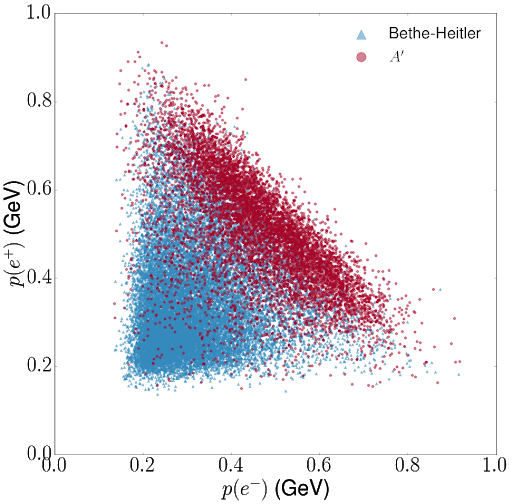
\includegraphics[width=0.5\textwidth]{figs/selection/p_vs_p.png}
%   \caption{p vs p}
%    \label{fig:km}
%\end{figure}

%\begin{figure}
%    \centering
%    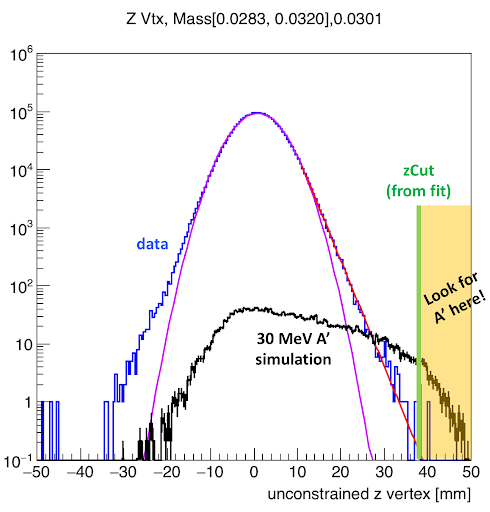
\includegraphics[width=0.5\textwidth]{figs/selection/mass_slice_2015.png}
%    \caption{Mass slice from 2015 \textcolor{red}{Replace this with the 2016 mass slice.}}
%    \label{fig:mass_slice}
%\end{figure}

\section{Previous Results from 2015 Engineering Run}\label{sec:2015vertexing}

The first displaced vertex search for $\aprime$s on HPS was performed on the 2015 Engineering Run \cite{adrian2018search}. As previously described, events were selected to eliminate prompt backgrounds that reconstruct downstream from the target where signal is expected, and the final event selection that was used in this analysis in both data and MC is shown in Fig. \ref{fig:2015eventselection}.

The final results of this analysis consist of estimating the expected number of signal events in the signal region and setting a limit on the $\aprime$ model. The maximum number of expected $\aprime$ events is 0.097 events at an $\aprime$ mass of 43.6 MeV and $\epsilon^2 = 2.4 \times 10^{-9}$. Unfortunately, this signal expectation is insufficient to set a limit on the canonical $\aprime$ model; however, a limit on a factor times the $\aprime$ cross-section can be set. The best limit set for this dataset is at an $\aprime$ mass of 51.4 MeV and $\epsilon^2=1.7 \times 10^{-9}$ in which an $\aprime$-like model with 35.7 times the cross-section is excluded with 90\% confidence at this point in parameter space.\footnote{One may be tempted to interpret this result as a simple scaling in luminosity. However, scaling luminosity also changes the signal region such that the expected $\aprime$ rate does not scale linearly. The exclusion of the $\aprime$ model times a certain factor of the cross-section is the better interpretation of this exclusion.} Though there is no known motivation for such a model, this provides an estimate for expected sensitivity for future runs. These final results are shown in Fig. \ref{fig:2015results}.

Even though the displaced vertex search from the 2015 Engineering Run did not provide a physically meaningful result, it provided essential information about backgrounds, particular those at high $z$. Through a detailed analysis of both the full dataset and in MC at truth level, it was determined that there were two main sources of high $z$ events. The first is due to large scatters in layer 1 of the tracker in which both $\epem$ particles have a large scatter away from the beam plane. This can either be a result of multiple Coulomb scattering, which dominates the cores and tails of the distribution, or from single Coulomb scattering whose angular scattering distributions have an even longer tail. These processes combined are a referred to as Moli\'ere scattering, and they can result in a vertex that is reconstructed far downstream from the target with a small error, and though most of these can be mitigated, a few of these processes are indistinguishable from a true displaced signal. Coulomb scattering in the first layer of the tracker remains the known fundamental limit of the experiment. 

The second main source of high $z$ backgrounds are due to mis-tracking in which the tracking algorithms pick up an incorrect hit in layer 1 (i.e. a hit that is not a result of the particle that produced the other hits on track), usually from a scattered beam particle, which pulls the vertex downstream. This situation is usually accompanied by a large scatter away from the beam plane by the other particle in the pair (even though it is tracked correctly) which results in a vertex reconstructed even further downstream. A schematic of these two backgrounds is shown in Fig. \ref{fig:2015backgrounds}. The knowledge obtained from this dataset was used to further improve the displaced vertex analysis for the 2016 Engineering Run.

\begin{figure}
    \centering
    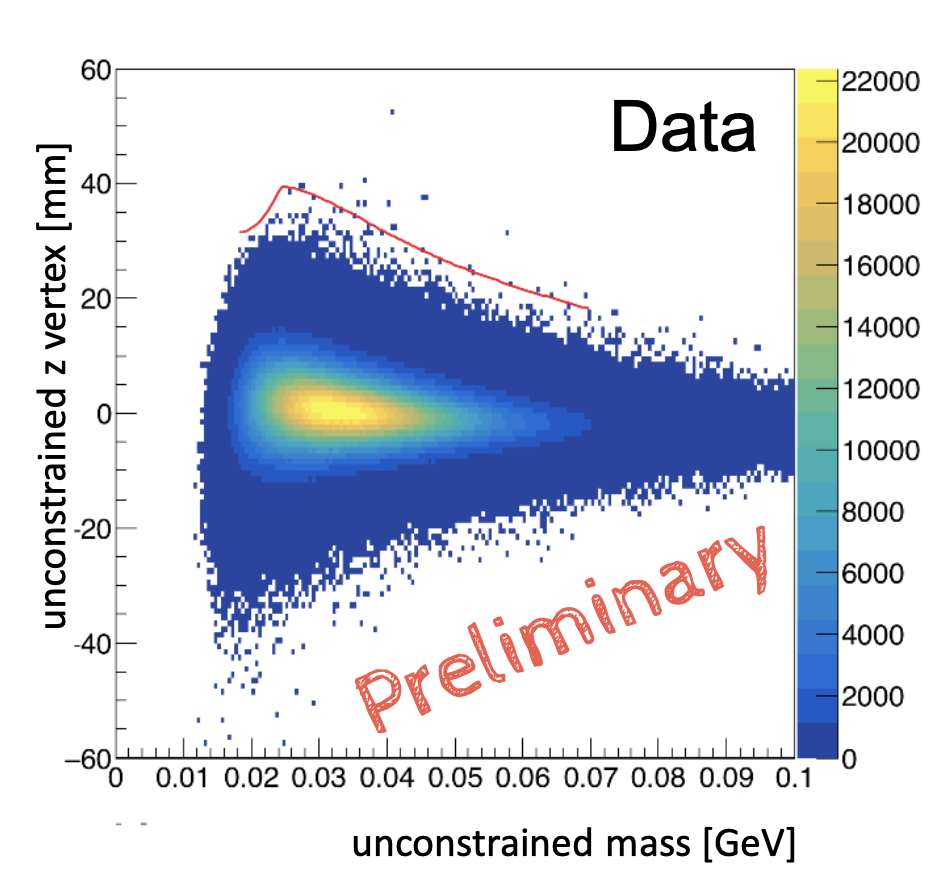
\includegraphics[width=0.45\textwidth]{figs/selection/data_final_2015.png}
    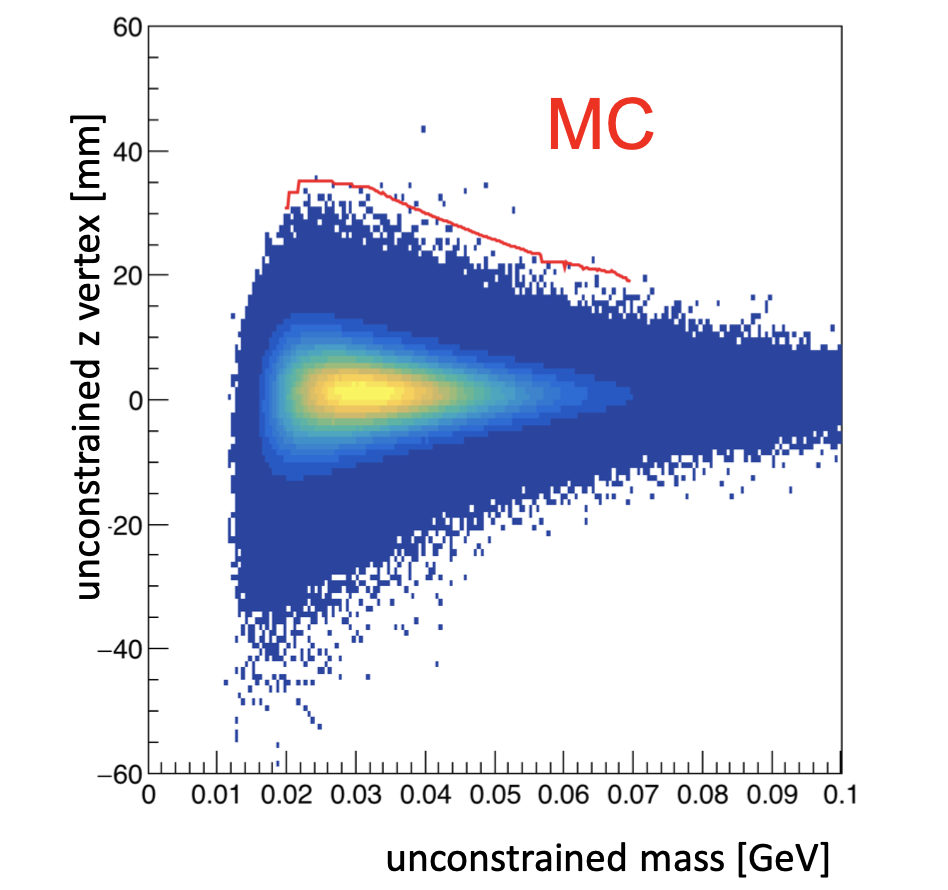
\includegraphics[width=0.45\textwidth]{figs/selection/mc_final_2015.png}
    \caption{Final event selection for the displaced vertex search in the 2015 Engineering Run for Left: Data and Right: a luminosity-equivalent tritrig-wab-beam MC sample. The $z_{cut}$ is shown in red.}
    \label{fig:2015eventselection}
\end{figure}

\begin{figure}
    \centering
    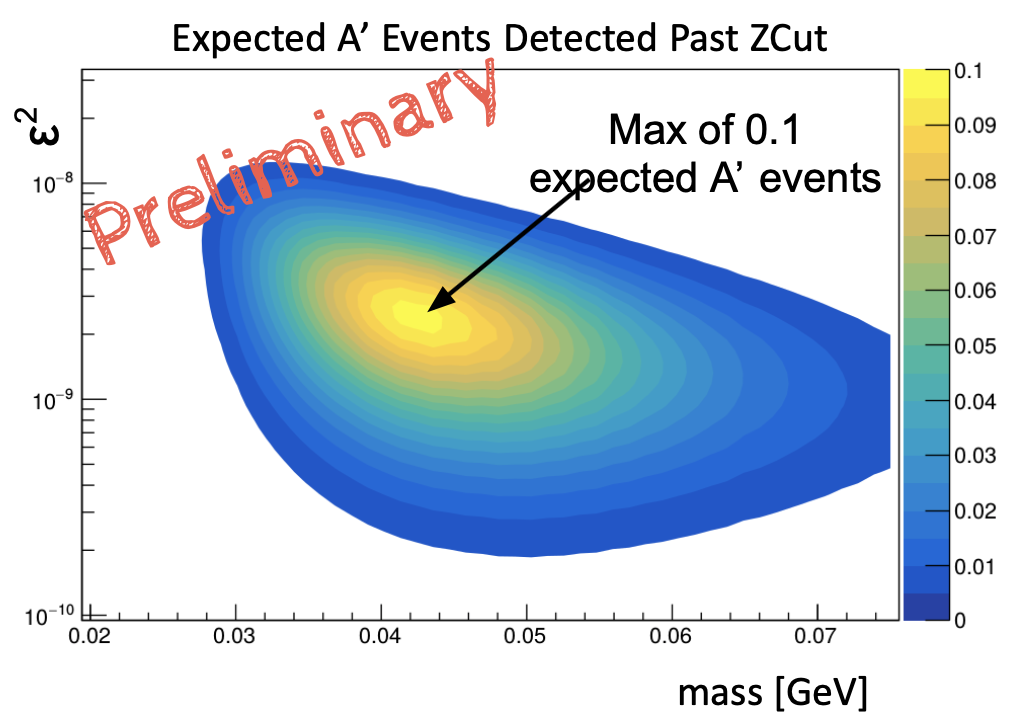
\includegraphics[width=0.45\textwidth]{figs/selection/detectable_2015.png}
    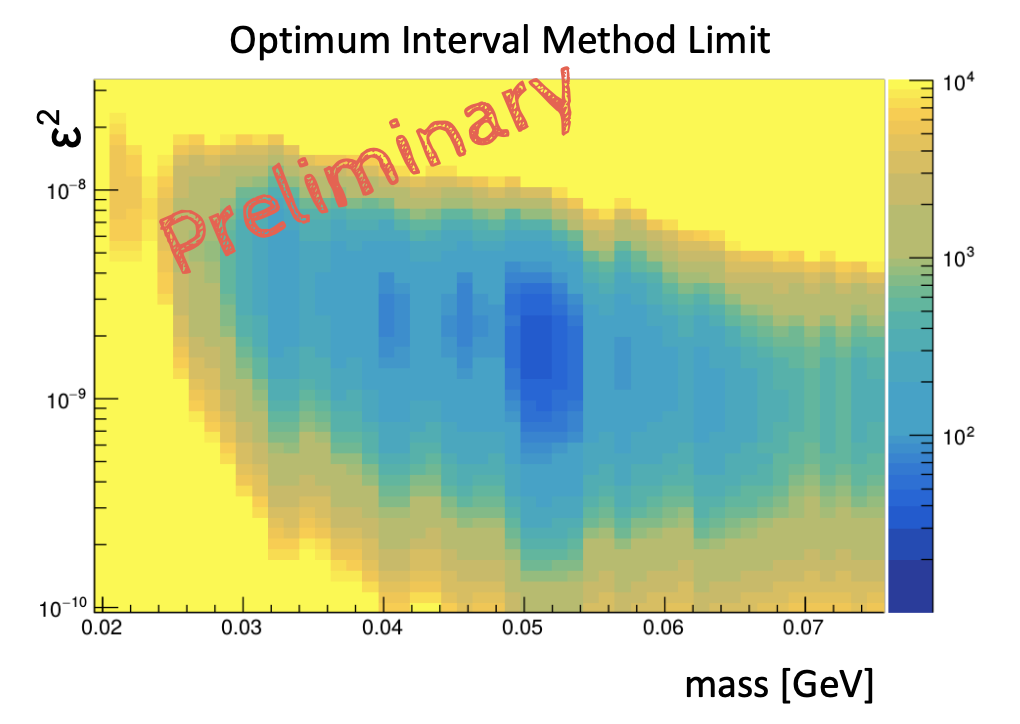
\includegraphics[width=0.45\textwidth]{figs/selection/oim_2015.png}
    \caption{Final results for the displaced vertex search for the 2015 Engineering Run. Left: The number of expected $\aprime$ events after all analysis cuts and $z_{cut}$ as a function of mass and $\epsilon^2$. The maximum number of expected $\aprime$ events is 0.097 events at an $\aprime$ mass of 43.6 MeV and $\epsilon^2 = 2.4 \times 10^{-9}$. Right: The limit on the $A'$ cross section as a function of mass and $\epsilon^2$ where the best limit set is at an $\aprime$ of 51.4 MeV and $\epsilon^2=1.7 \times 10^{-9}$ in which an $\aprime$-like model with 35.7 times the cross-section is excluded with 90\% confidence.}
    \label{fig:2015results}
\end{figure}

\begin{figure}
    \centering
    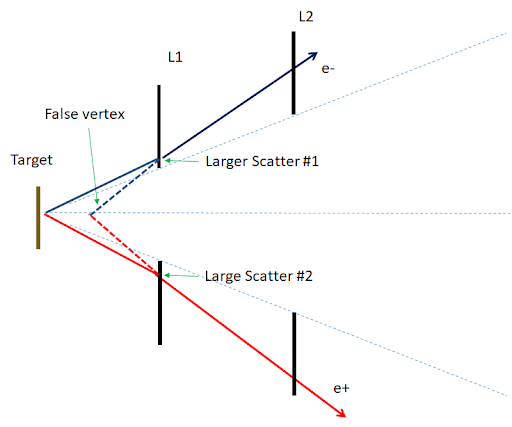
\includegraphics[width=0.45\textwidth]{figs/selection/large_scatter_bg.png}
    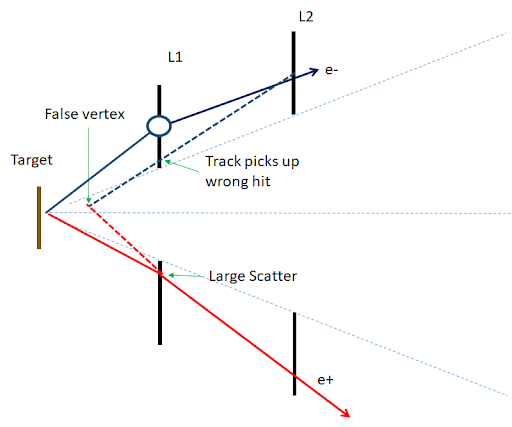
\includegraphics[width=0.45\textwidth]{figs/selection/iso_bck.png}
    \caption{From detailed MC studies, it was shown that the backgrounds are due to two main processes. We seek to further mitigate these backgrounds in the 2016 Engineering Run. Left: A vertex is falsely reconstructed downstream of the target due to two large scatters of the $\epem$ pairs away from the beam plane. Right: A vertex is falsely reconstructed downstream of the target due to a track picking up the incorrect layer 1 hit (mis-tracking). These events are usually accompanied by a large scatter in the other particle that is tracked correctly.}
    \label{fig:2015backgrounds}
\end{figure}

\clearpage

\section{Mass Resolution}\label{sec:massresolution}

The displaced vertex search is performed in bins of reconstructed mass for a given $A'$ mass hypothesis. In order to accurately estimate the expected $A'$ yield in a given mass bin, it is important to have an accurate estimate of the mass resolution as a function of mass in order to compute the amount of signal yield by searching in a finite mass window. The uncertainty of the mass resolution can result in more signal leaking out of a given mass bin than into the bin and is a source of systematic uncertainty described in Sec. \ref{sec:systematics}. 

In order to provide a standard mass point directly from data, the invariant mass of scattered $e^-e^-$ M\o ller pairs (known as a function of energy) are used. However, unfortunately, comparing the mass resolution for M\o llers between data and MC shows dramatically different results which can be attributed to the observed discrepancy between the momentum resolutions in the data and the MC. In order to account for this, the momentum of the tracks is smeared and the mass resolution is re-scaled. Lastly, the mass resolution is shown to be independent of decay length, thus the mass resolution for a given $A'$ mass can be kept constant.%More details on the mass resolution are shown in the 2016 Resonance Search note (\textcolor{red}{cite BH note}).

\subsection{M\o ller Event Selection}

M\o llers, that is elastically-scattered $e^-e^-$ pairs, provide a convenient standard mass point for HPS. The invariant mass of M\o llers is a function of beam energy and can be computed from the  total energy in the center of mass frame at a beam energy of 2.3 GeV.

\begin{equation}
    M(\mathrm{e}^{-}\mathrm{e}^{+}) = \sqrt{S_{\mathrm{cm}} } = \sqrt{ 2m_{\mathrm{e}^{-}}^{2} + 2E_{\mathrm{beam}}m_{\mathrm{e}^{-}} } \approx \sqrt{ 2E_{\mathrm{beam}}m_{\mathrm{e}^{-}} } = 48.498\mathrm{MeV}
    \label{eq:MlrCmEnergy}
\end{equation}

%The M\o ller event selection is shared with the resonance search and more details are discussed in the analysis note (\textcolor{red}{cite BH note}). Similar to how V0 candidates are constrained differently between the resonance search and the displaced vertex search, the main difference for the vertex formed by electron pairs is the target constraint for the resonance search and unconstrained for the displaced vertex search. 

The basic selection involves choosing $e^-e^-$ pairs in opposite detector volumes within a small time window and in a fiducial region of the Ecal. These selections reduce the backgrounds due to out of time electrons and electrons which scatter elastically off the target. However, at this beam energy the moller mass results in an opening angle that is near the edge of the HPS acceptance, and it is rare for both electrons to fall within the acceptance of the Ecal.\footnote{M\o llers are selected using a pre-scaled single cluster trigger, so at least one electron must interact with the Ecal.} The electron that does not interact with the Ecal often times falls into the so-called ``Ecal hole'' where 5 crystals on both top and bottom halves were removed to reduce occupancy from elastically-scattered beam particles. Despite this, both electrons can be within the tracker acceptance since the tracker acceptance still covers the acceptance over the Ecal hole. 

Thus, the M\o ller event selection must be track-based using both the track times and the extrapolation of the track to the face of the Ecal. The variables used for the event selection include the track time difference ($\Delta t$), the momentum sum of the $\epem$ pair ($P_{sum}$), and the difference between the extrapolated track $x$ position to the Ecal face and the Ecal cluster $x$ position ($\Delta x$). Unfortunately, the MC does not accurately describe the observed track extrapolation resolution or the track time resolution, so different cuts must be used for data and MC, thus a different set of cuts is utilized between the them. The M\o ller event selection for data is summarized in Table \ref{tab:moller_data}, and the MC M\o ller event selection is summarized in Table \ref{tab:moller_MC}. The M\o ller mass resolution for data, MC, and MC with track momentum smearing (described in the next section) using the unconstrained $e^-e^-$ vertex is shown in Fig. \ref{fig:moller_mass_fit}.

\begin{table}[t] 
    \centering
    \begin{tabular}{lr}
        \toprule
        \textbf{Cut Description} & \textbf{Requirement} \\
        \midrule
        Time Difference Min & $\Delta t>-2.94$ ns\\
        Time Difference Max & $\Delta t<1.69$ ns\\
        $P_{sum}$ Min & $P_{sum}>2.0$ GeV\\
        $P_{sum}$ Max & $P_{sum}<2.45$ GeV\\
        $\Delta x_{top}$ Min & $\Delta x_{top}>-4.72$ mm\\
        $\Delta x_{top}$ Max & $\Delta x_{top}<6.15$ mm\\
        $\Delta x_{bot}$ Min & $\Delta x_{bot}>-7.51$ mm\\
        $\Delta x_{bot}$ Max & $\Delta x_{bot}<2.98$ mm\\
        \bottomrule
    \end{tabular}
    \caption{M\o ller event selection for data on $e^-e^-$ pairs. Since electron tracks are not required to match to Ecal clusters, the time difference is between track times and position differences are based on track extrapolations to the Ecal.}
    \label{tab:moller_data}
\end{table}

\begin{table}[t] 
    \centering
    \begin{tabular}{lr}
        \toprule
        \textbf{Cut Description} & \textbf{Requirement} \\
        \midrule
        Time Difference Min & $\Delta t>-1.44$ ns\\
        Time Difference Max & $\Delta t<1.54$ ns\\
        $P_{sum}$ Min & $P_{sum}>2.15$ GeV\\
        $P_{sum}$ Max & $P_{sum}<2.42$ GeV\\
        $\Delta x_{top}$ Min & $\Delta x_{top}>-4.89$ mm\\
        $\Delta x_{top}$ Max & $\Delta x_{top}<4.82$ mm\\
        $\Delta x_{bot}$ Min & $\Delta x_{bot}>-4.98$ mm\\
        $\Delta x_{bot}$ Max & $\Delta x_{bot}<4.52$ mm\\
        \bottomrule
    \end{tabular}
    \caption{M\o ller event selection for MC on $e^-e^-$ pairs. Since electron tracks are not required to match to Ecal clusters, the time difference is between track times and position differences are based on track extrapolations to the Ecal.}
    \label{tab:moller_MC}
\end{table}

\begin{figure}[!hb]
    \centering
    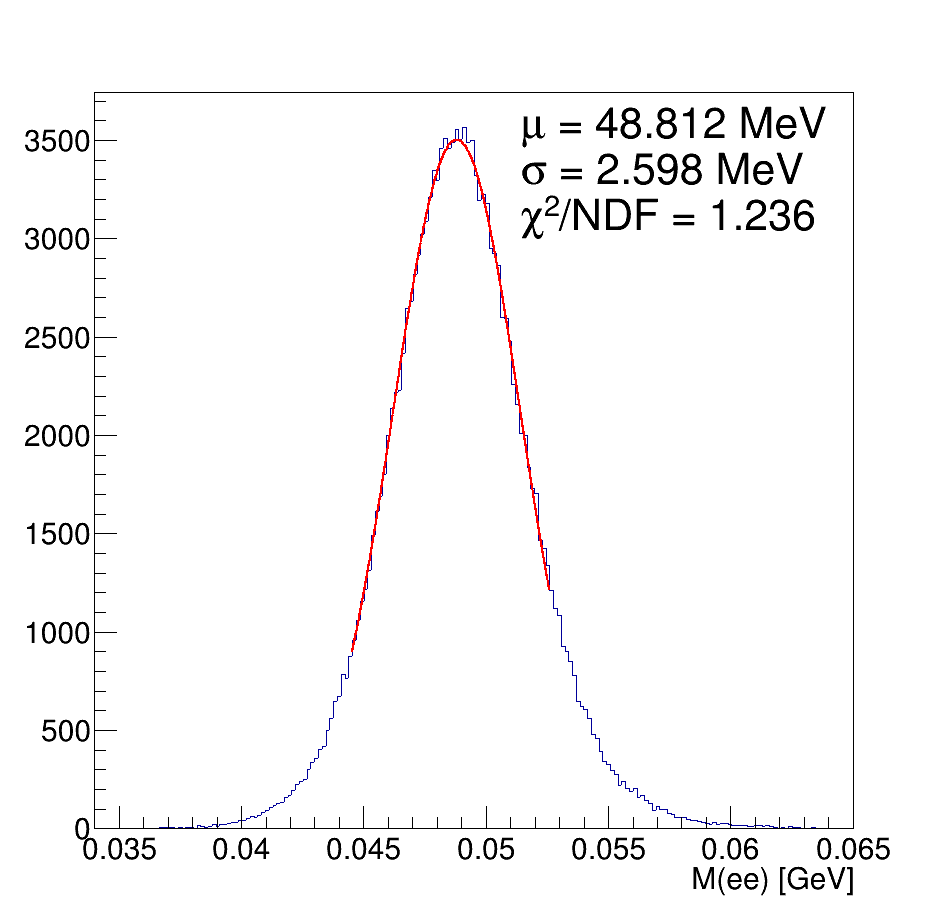
\includegraphics[width=.45\textwidth]{figs/selection/mlr_recmassscsmfit_data_unconstrained.png}
    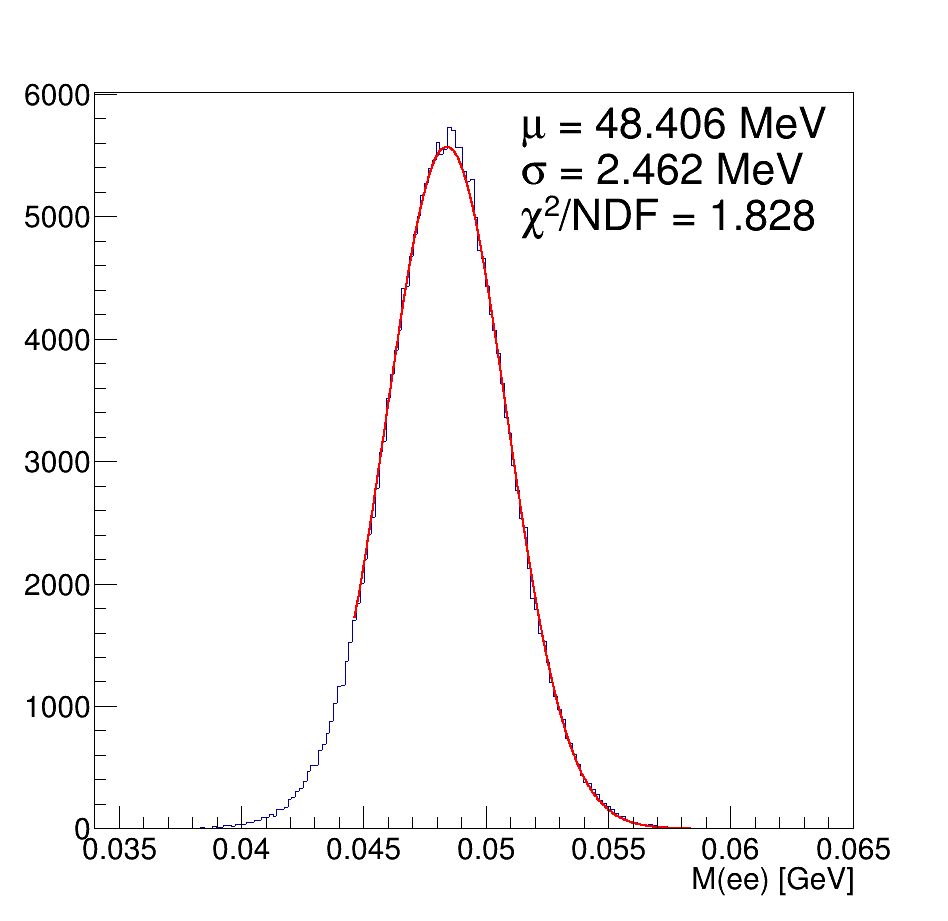
\includegraphics[width=.45\textwidth]{figs/selection/mlr_recmassscsmfit_mc_unconstrained.png}
    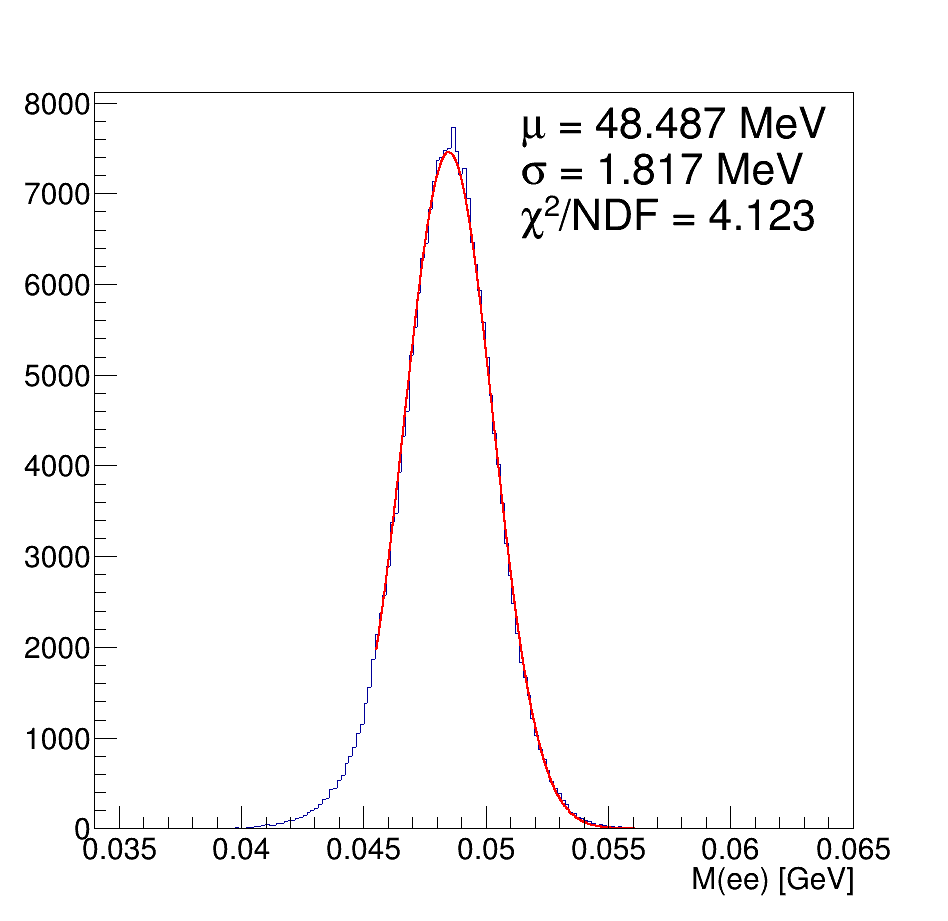
\includegraphics[width=.45\textwidth]{figs/selection/mlr_recmassfit_mc_unconstrained.png}
    \caption{Fitted $e^-e^-$ spectrum using the M\o ller selection for Upper Left: Data, Upper Right: M\o ller MC with track momentum smearing, and Bottom: M\o ller MC.
    }
    \label{fig:moller_mass_fit}
\end{figure}

\clearpage

\subsection{Corrected Mass Resolution}

As stated previously, there is a discrepancy in the M\o ller mass resolution between data and MC that can be attributed to the difference in momentum resolution of individual tracks which is $\sim20$\%. To approximate the effect of a momentum resolution difference on the mass resolution discrepancy, a small-angle approximation for the opening angle can be used. The invariant mass and mass resolution is given by
\begin{equation}
    M_{\epem} = 2 \sqrt{p_1 p_2} \ \mathrm{sin} \left( \frac{\theta}{2} \right) \sim \frac{1}{\sqrt{2}}\theta \sqrt{p_{1}p_{2}}
\end{equation}
\begin{equation}
    \sigma_m = \frac{1}{\sqrt{2}} \theta \frac{\sqrt{p_{1}p_{2}}}{2}
        \left( \frac{\sigma_{p_1}}{p_1} + \frac{\sigma_{p_2}}{p_2} 
        + \sigma_{\theta} \sqrt{p_{1}p_{2}} \right)
    \label{equ:mass_res}
\end{equation}
From equation \ref{equ:mass_res}, it can be seen that a 20\% increase in momentum resolution results in an increase of $\sim 20\%$ in mass resolution,  which would largely account for much of the mass resolution discrepancy (the angular resolution discrepancy is small and can be ignored). 

In order to correct for this discrepancy, a smearing technique on the track momentum is utilized and the mass resolution is re-scaled. This smearing method involves throwing a random number Gaussianly distributed about zero, such that when added in quadrature with the momentum as measured (and of a known resolution), the new MC momentum resolution estimate agrees with the data momentum resolution. %With the new smeared momentum, the mass resolution is re-computed and shows agreement with the M\o ller mass resolution in data.

%This smearing factor is calculated using the discrepancy between the data and MC full-energy electron (FEE) momentum distributions where a narrow peak near the beam energy is expected. The smearing factor deconvolutes the difference in Gaussian widths of data and MC such that the widths agree when smearing. 

It is assumed that the relative momentum discrepancy does not change appreciably with particle momentum. The factor used for momentum smearing is a function of detector hemisphere and the number of hits on track. These factors are used to smear momentum on a track-by-track basis and the resulting smeared momentum is denoted as $p_{1,sm}$ and $p_{2,sm}$. From the smeared momentum, the invariant mass can be re-scaled using the original momenta and mass.

\begin{equation}
    M_{e^-e^-,sm} = 2 \sqrt{p_{1}p_{2}} \ \mathrm{sin} \left( \frac{\theta}{2} \right) = 2 \sqrt{\frac{p_{1,sm}}{p_{1}} p_{1} \frac{p_{2,sm}}{p_{2}} p_{2} }  \ \mathrm{sin} \left( \frac{\theta}{2} \right) = \sqrt{\frac{p_{1,sm}}{p_{1}} \frac{p_{2,sm}}{p_{2} }} M_{e^-e^-}
    \label{equ:mass_res_smear}
\end{equation}

This smeared invariant mass $M_{e^-e^-,sm}$ is then refit with a Gaussian distribution, the width of which is the smeared mass resolution. This smeared mass resolution is in excellent agreement with data over the entire mass range of interest.

An example of a 100 MeV displaced $A'$ in the L1L1 category comparing the MC with and without momentum smearing as well as the decay length dependence is shown in Fig. \ref{fig:mass_resolution_L1L1}.\footnote{The three mutually exclusive categories - L1L1, L1L2, and L2L2 - are described in Sec. \ref{sec:acceptance}.} %An example of a 100 MeV displaced $A'$ in the L1L2 category comparing the MC with and without momentum smearing as well as the decay length dependence is shown in Fig. \ref{fig:mass_resolution_L1L2}. 
In general, there is little dependence of the mass resolution on the decay length including in the L1L2 category. The momentum measurement depends on the measurement and multiple Coulomb scattering errors and the number and positions of hit layers, not just layers 4-6. But, it does not depend on the $z$-position of the decay.

%This is because the precision of the momentum measurement, and hence the mass resolution, is a result of the final layers of the SVT (layers 4 - 6) where the curvature of charged particles is maximum and can be more precisely measured. Thus, mass resolution is a function of the number of layers hit, not of the decay position.% or which layer the particles hit first.

Because of this, prompt $A'$s can be used which offer an advantage of more statistics particularly at low mass. In addition, for simplicity, the same cuts as the radiative fraction in Table \ref{tab:radfrac} with the appropriate layer requirements are used to determine the mass resolution as any further cuts are used to eliminate falsely reconstructed vertices downstream of the target and have little effect on the core of the distribution.

The mass resolution for both the L1L1 and L1L2 categories is shown in Fig. \ref{fig:mass_resolution}.\footnote{For the L1L2 category, prompt $\aprime$s are still used; however, the difference between the L1L1 category is the ratio of the 5-hit to 6-hit tracks. Since momentum smearing depends on the number of hits on track, the proper fraction of 5-hit tracks is used and is dependent on mass.} These plots make a comparison between the M\o ller mass resolution in data and MC as well as the MC with the momentum smearing technique. As expected, the MC M\o ller mass resolution is underestimated significantly; however, once the momentum smearing is incorporated agrees well with data. In previous analysis of the 2015 Engineering Run, the mass resolution was re-scaled by a constant factor of the ratio between the data to MC M\o ller mass resolution. However, there is clear evidence that this method underestimates the mass resolution, thus the smearing technique is utilized.\footnote{There is a mass point in which the unconstrained mass resolution is better than the target constrained mass resolution used in the resonance search. This is clearly absurd and is a good indication that simply scaling the mass resolution is insufficient.} These plots also compare the $\aprime$ mass resolution with both the scaling and smearing techniques.

%The mass resolution for both the L1L1 and L1L2 categories comparing MC, MC scaled by the M\o ller mass resolution in data and MC, and MC with track momentum smearing is shown in Fig. \ref{fig:mass_resolution}.\footnote{For the L1L2 category, prompt $\aprime$s are still used; however, the difference between the L1L1 category is the ratio of the 5-hit to 6-hit tracks. Since momentum smearing depends on the number of hits on track, the proper fraction of 5-hit tracks is used and is dependent on mass.}

Lastly, the mass resolution is parametrized as a function of mass using a 4th order polynominal fit to the mass resolution with track momentum smearing. This parameterization is used as an input to the size of the mass search windows. For L1L1, the parametrization is

\begin{equation}
    %\sigma_m(m) = 0.01095 \mathrm{MeV} + 0.04395 m
    \sigma_m(m\mathrm{[MeV]}) = 0.9348 + 0.05442 \ m -5.784\times 10^{-4} \ m^2 + 5.852\times 10^{-6} \ m^3 - 1.724\times 10^{-8} \ m^4
    \label{eq:mres_L1L1}
\end{equation}

and for L1L2, the parametrization is

\begin{equation}
    %\sigma_m(m) = 0.01095 \mathrm{MeV} + 0.04395 m
    \sigma_m(m\mathrm{[MeV]}) = 0.8427 + 0.04709 \ m -2.067\times 10^{-4} \ m^2 + 2.087\times 10^{-6} \ m^3 - 5.584\times 10^{-9} \ m^4
    \label{eq:mres_L1L2}
\end{equation}

%\begin{equation}
%    \sigma_m(m) = 0.04906 \mathrm{MeV} + 0.04694 m
%    \label{eq:mres_L1L2}
%\end{equation}

\begin{figure}[!hb]
    \centering
    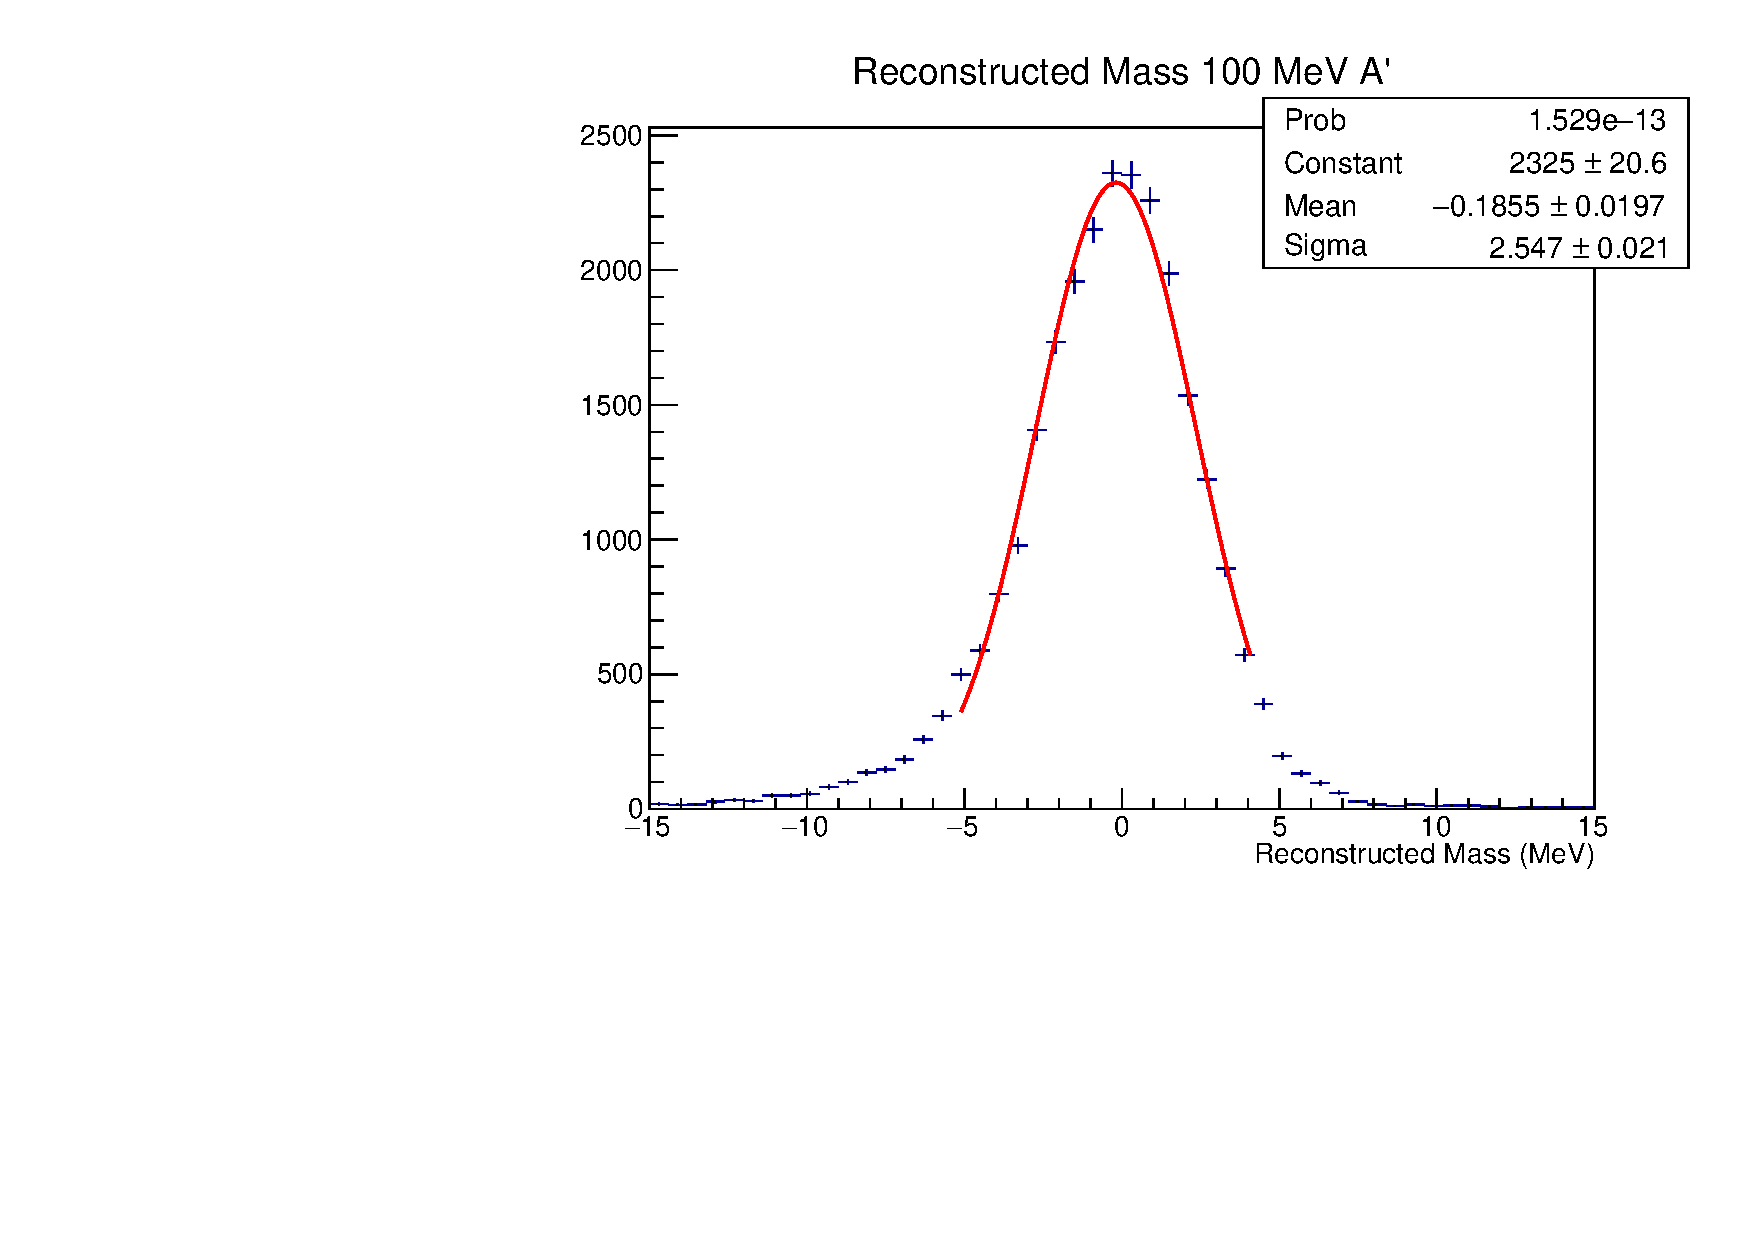
\includegraphics[width=.45\textwidth]{figs/selection/massResL1L1_ap100MeV.pdf}
    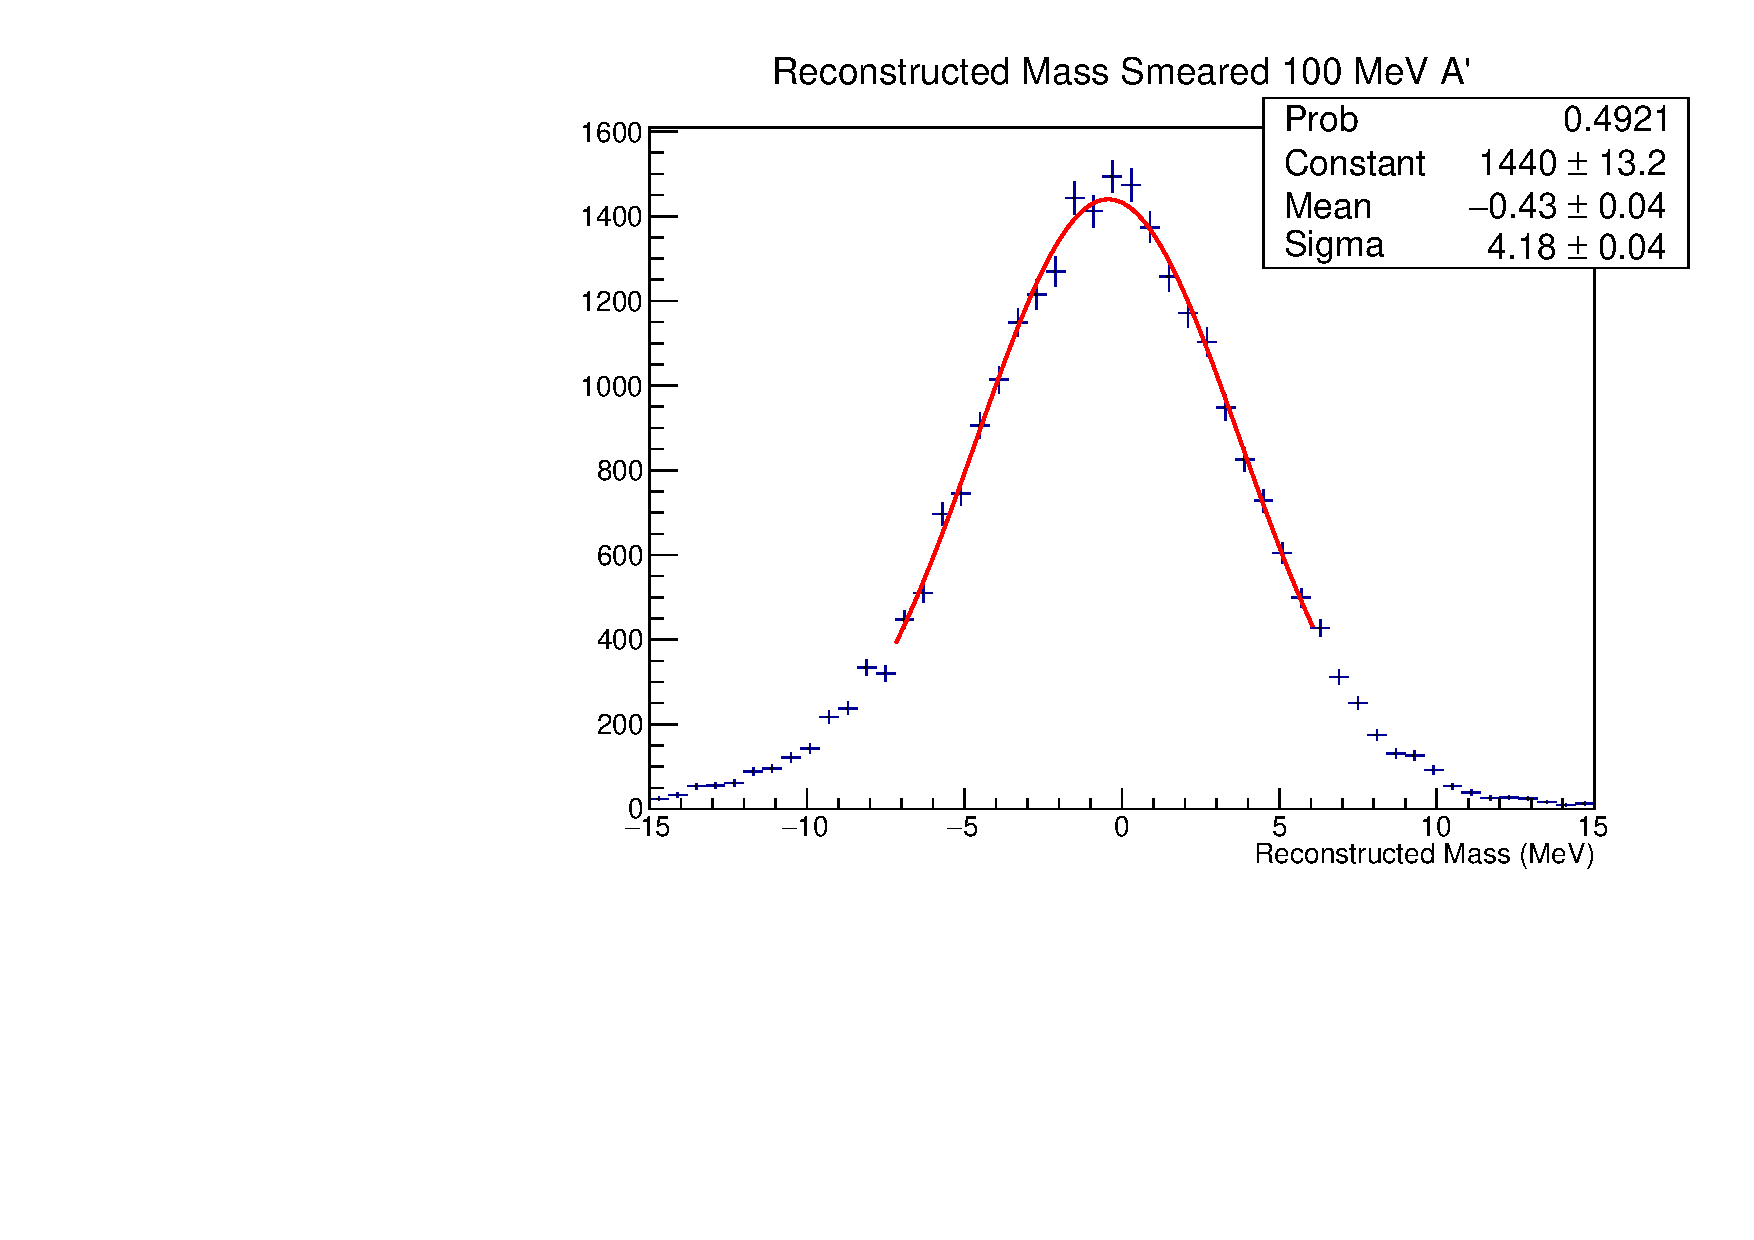
\includegraphics[width=.45\textwidth]{figs/selection/massResL1L1_ap100MeV_smeared.pdf}
    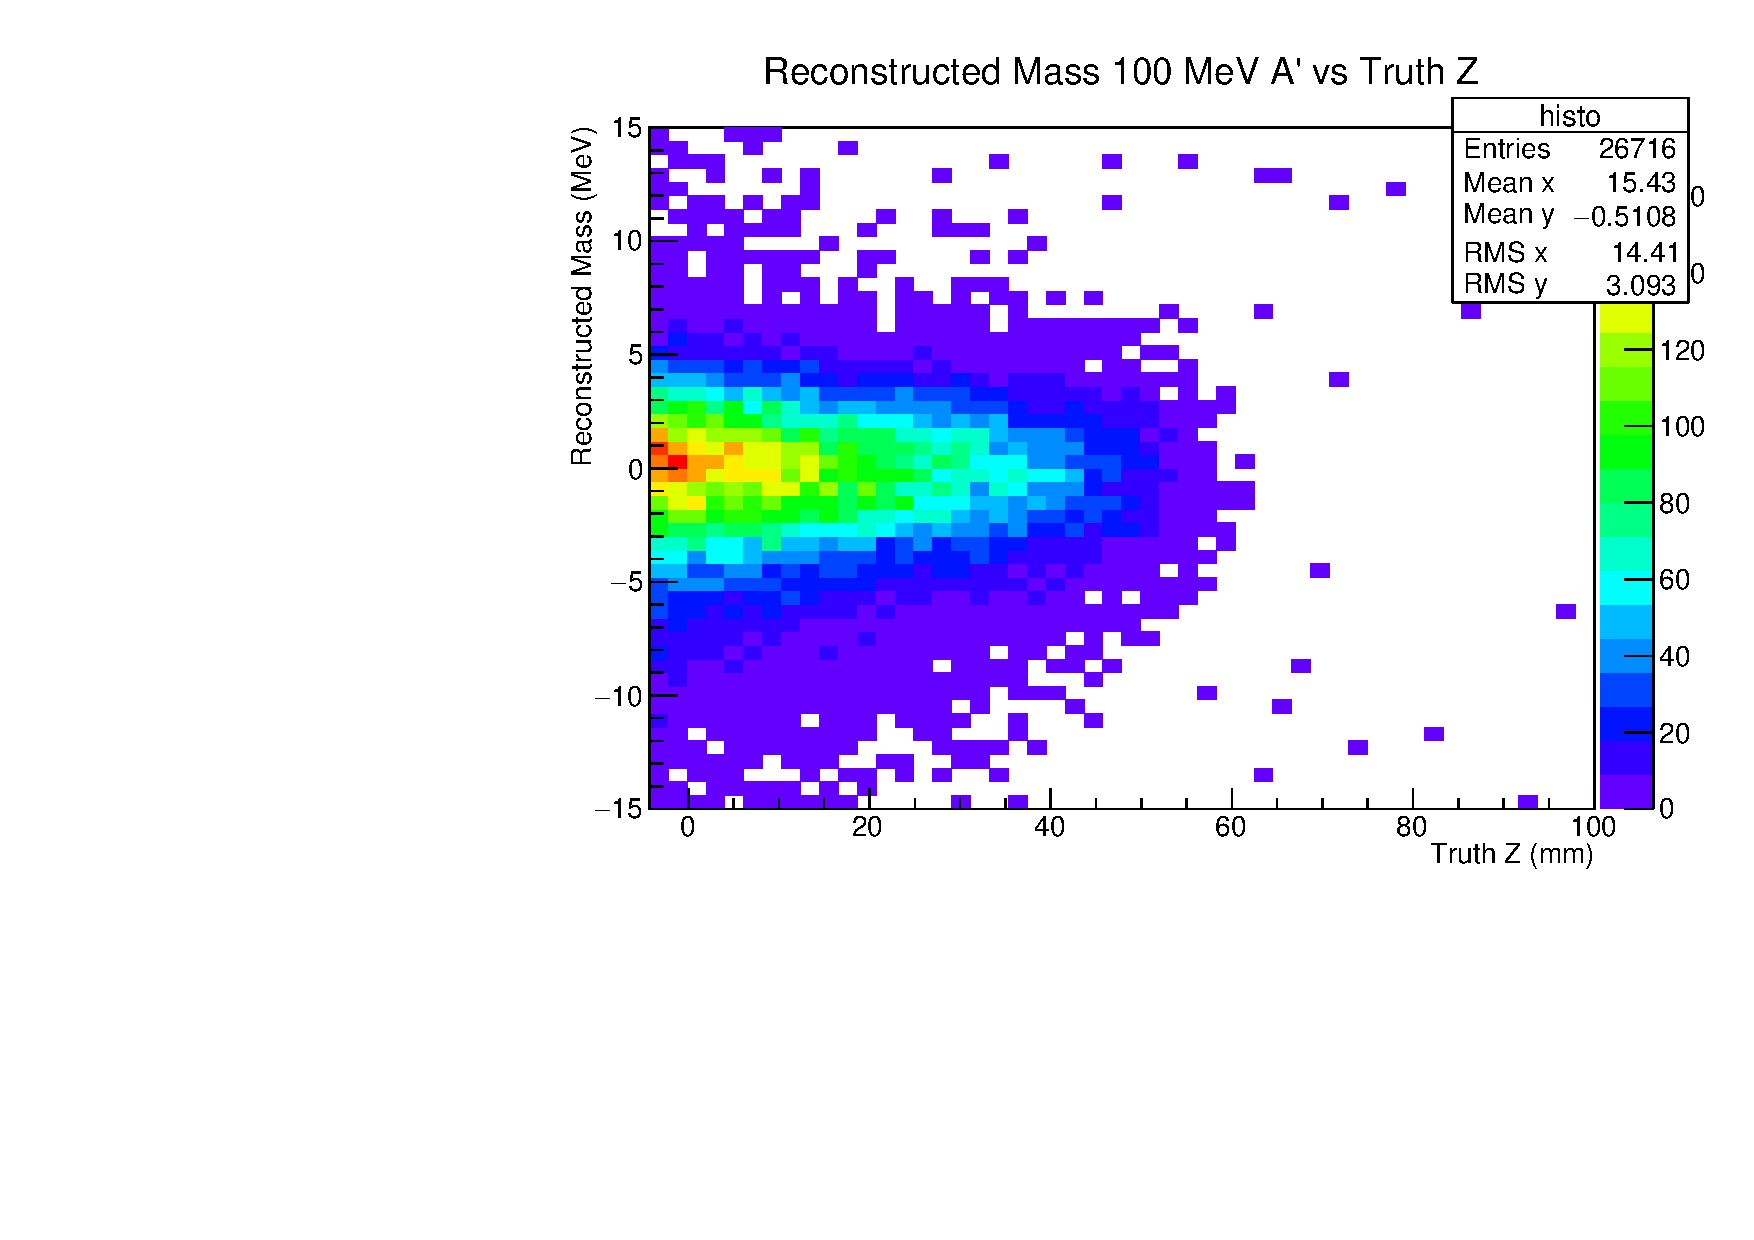
\includegraphics[width=.45\textwidth]{figs/selection/massResL1L1_ap100MeV_m_z.pdf}
    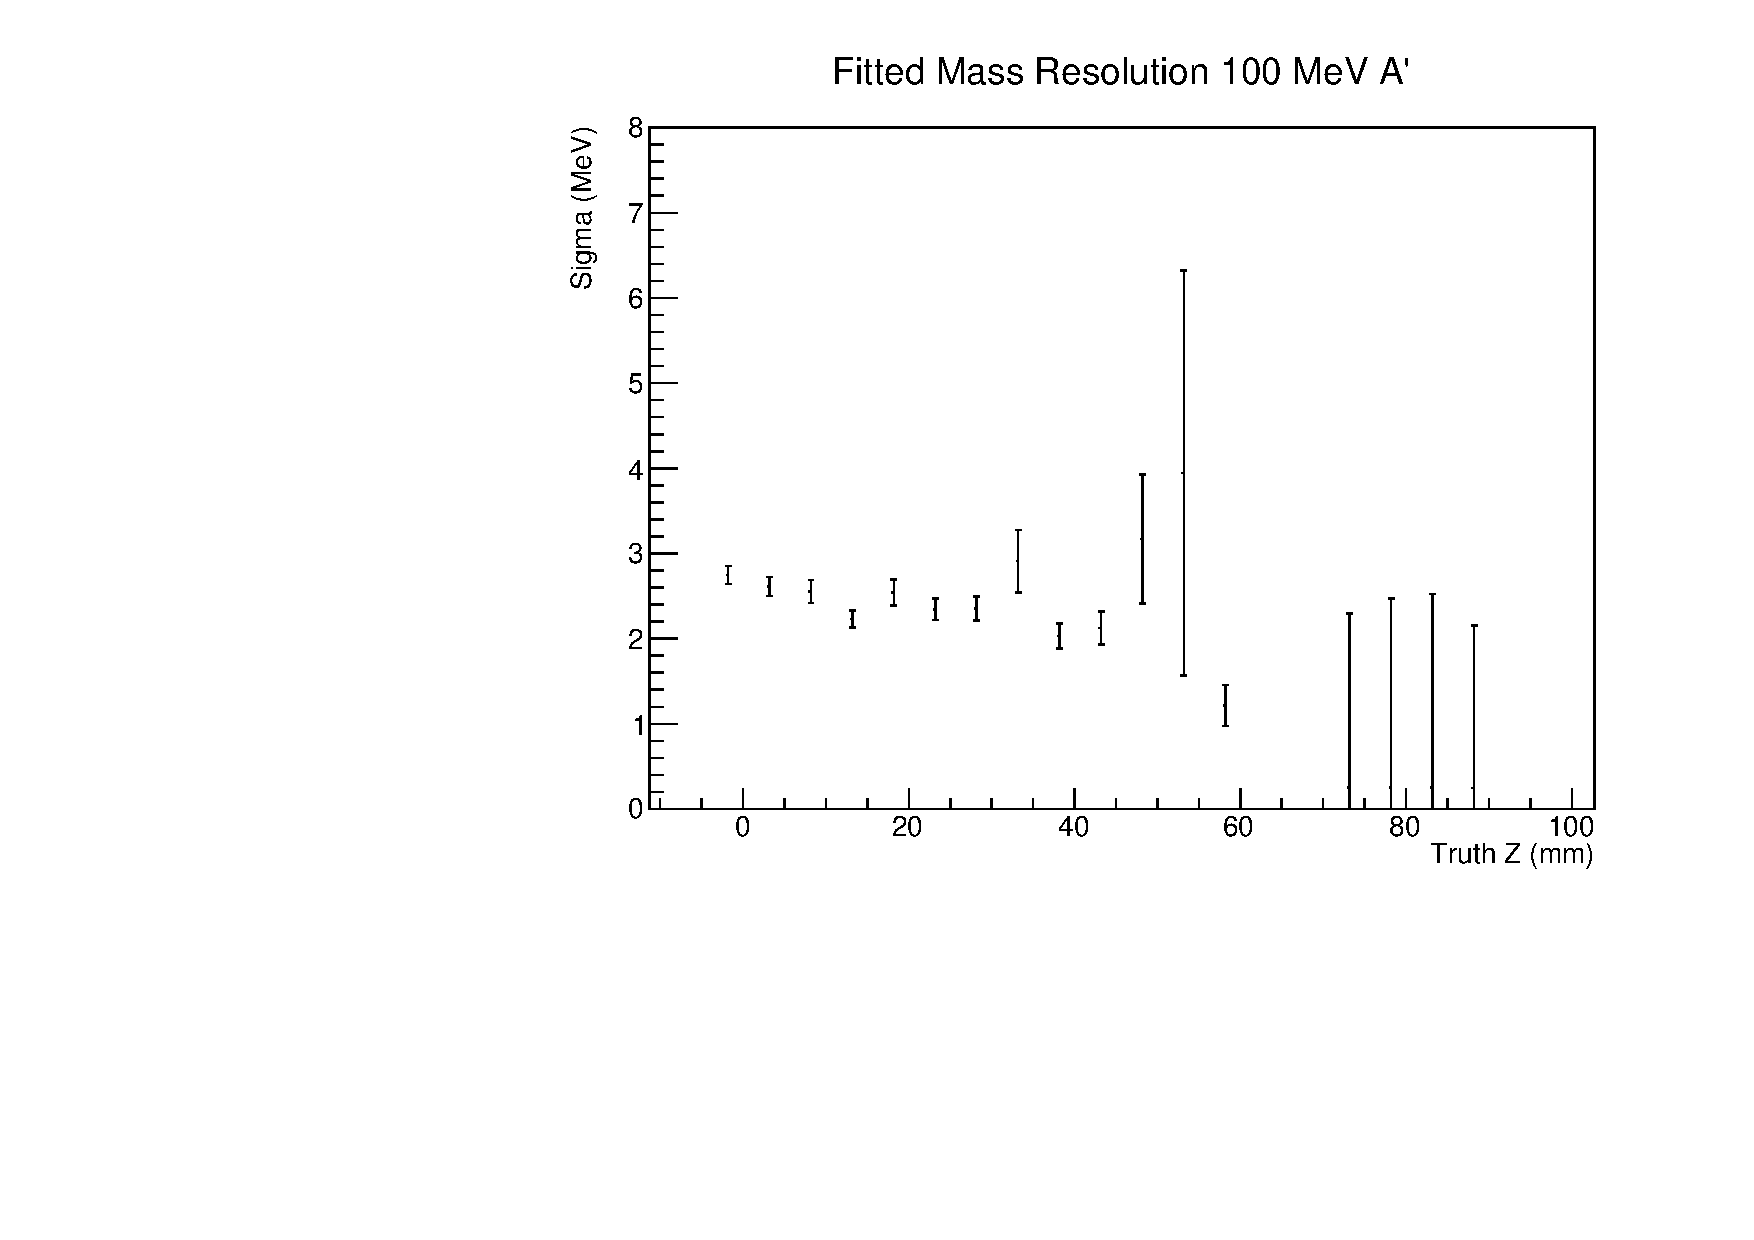
\includegraphics[width=.45\textwidth]{figs/selection/massResL1L1_ap100MeV_z.pdf}
    \caption{Upper Left: Fitted reconstructed mass spectrum for a 100 MeV displaced $A'$. Upper Right: Fitted reconstructed mass spectrum for a 100 MeV displaced $A'$ with track momentum smearing. Lower Left: Reconstructed mass vs truth $z$ decay for a 100 MeV displaced $A'$. Lower Right: The fitted mass resolution for 100 MeV displaced $A'$s as in slices of truth $z$. Mass resolution is approximately  independent of decay length. These plots are for the L1L1 category.
    }
    \label{fig:mass_resolution_L1L1}
\end{figure}

%\begin{figure}[!hb]
%    \centering
%    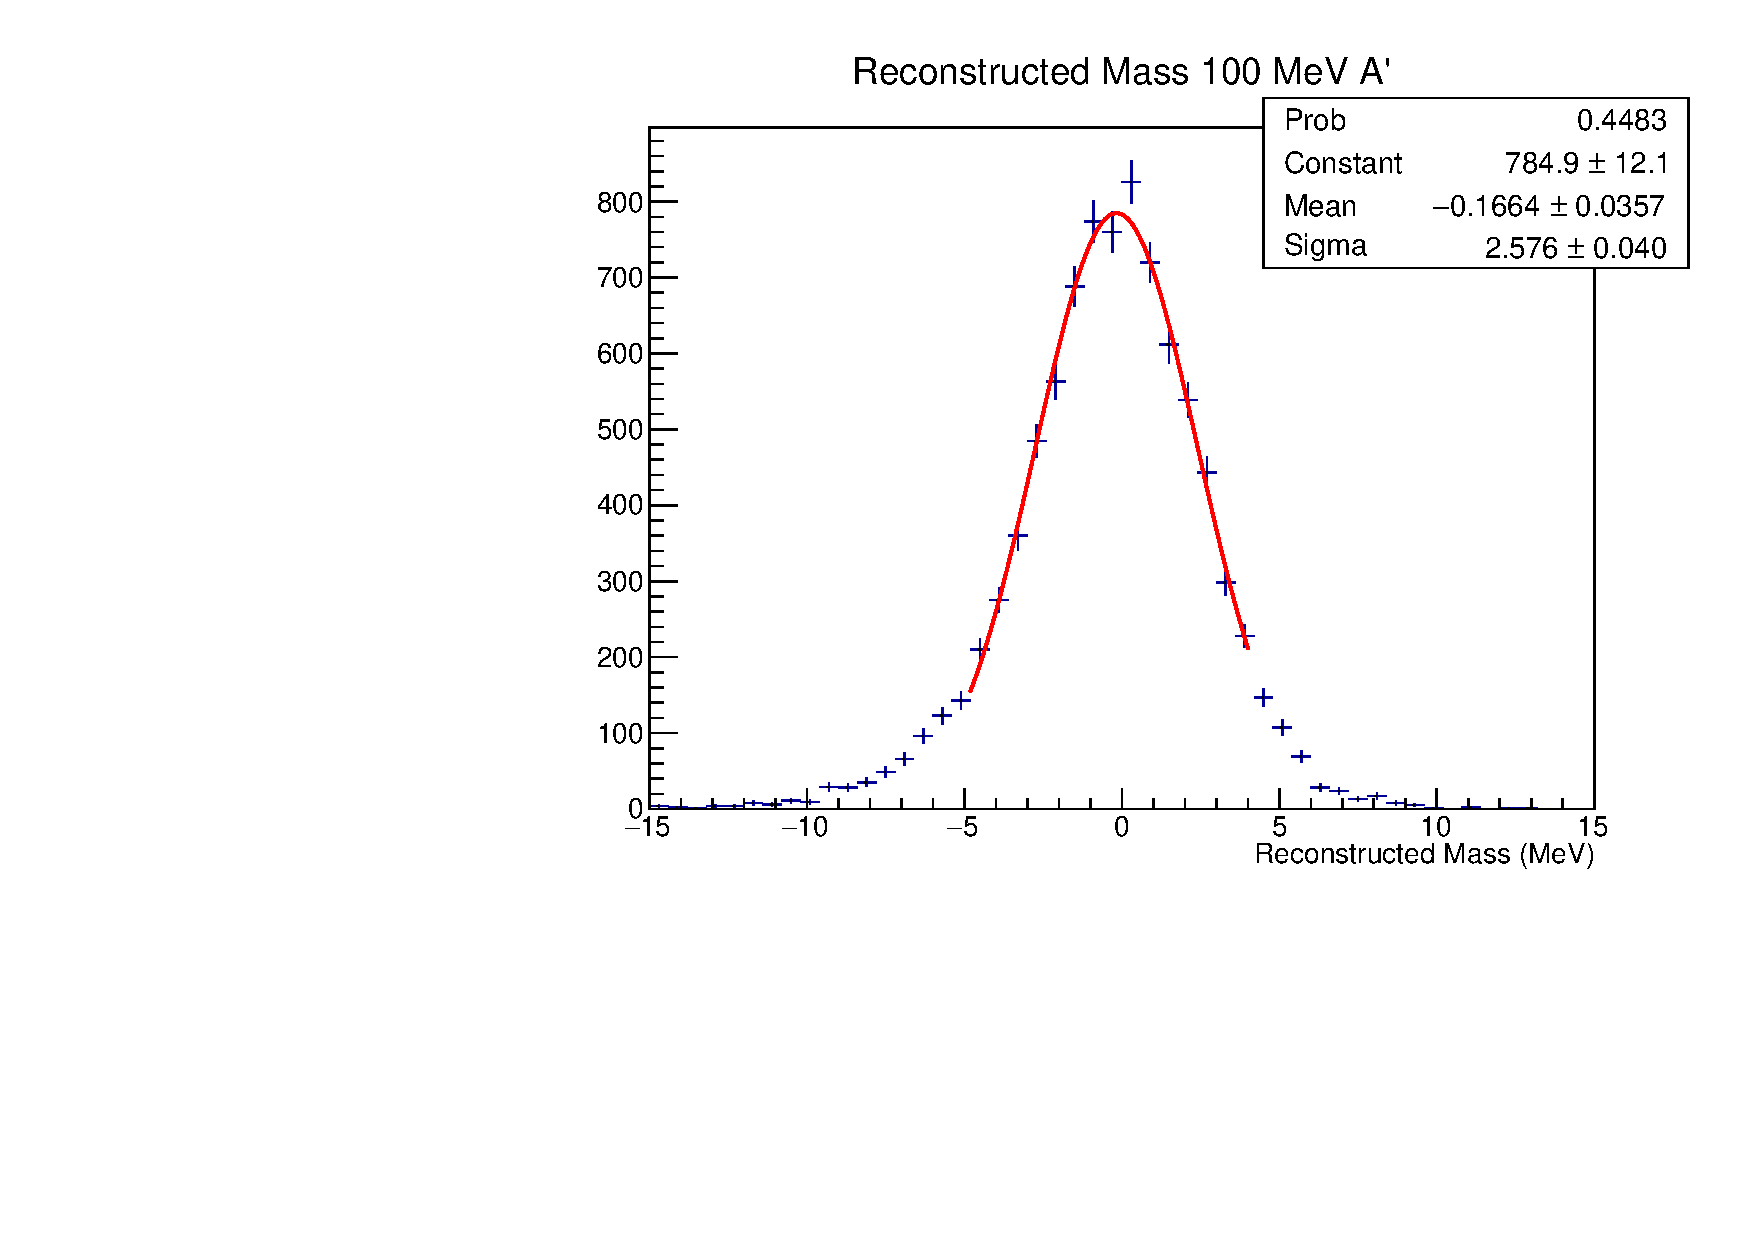
\includegraphics[width=.45\textwidth]{figs/selection/massResL1L2_ap100MeV.pdf}
%    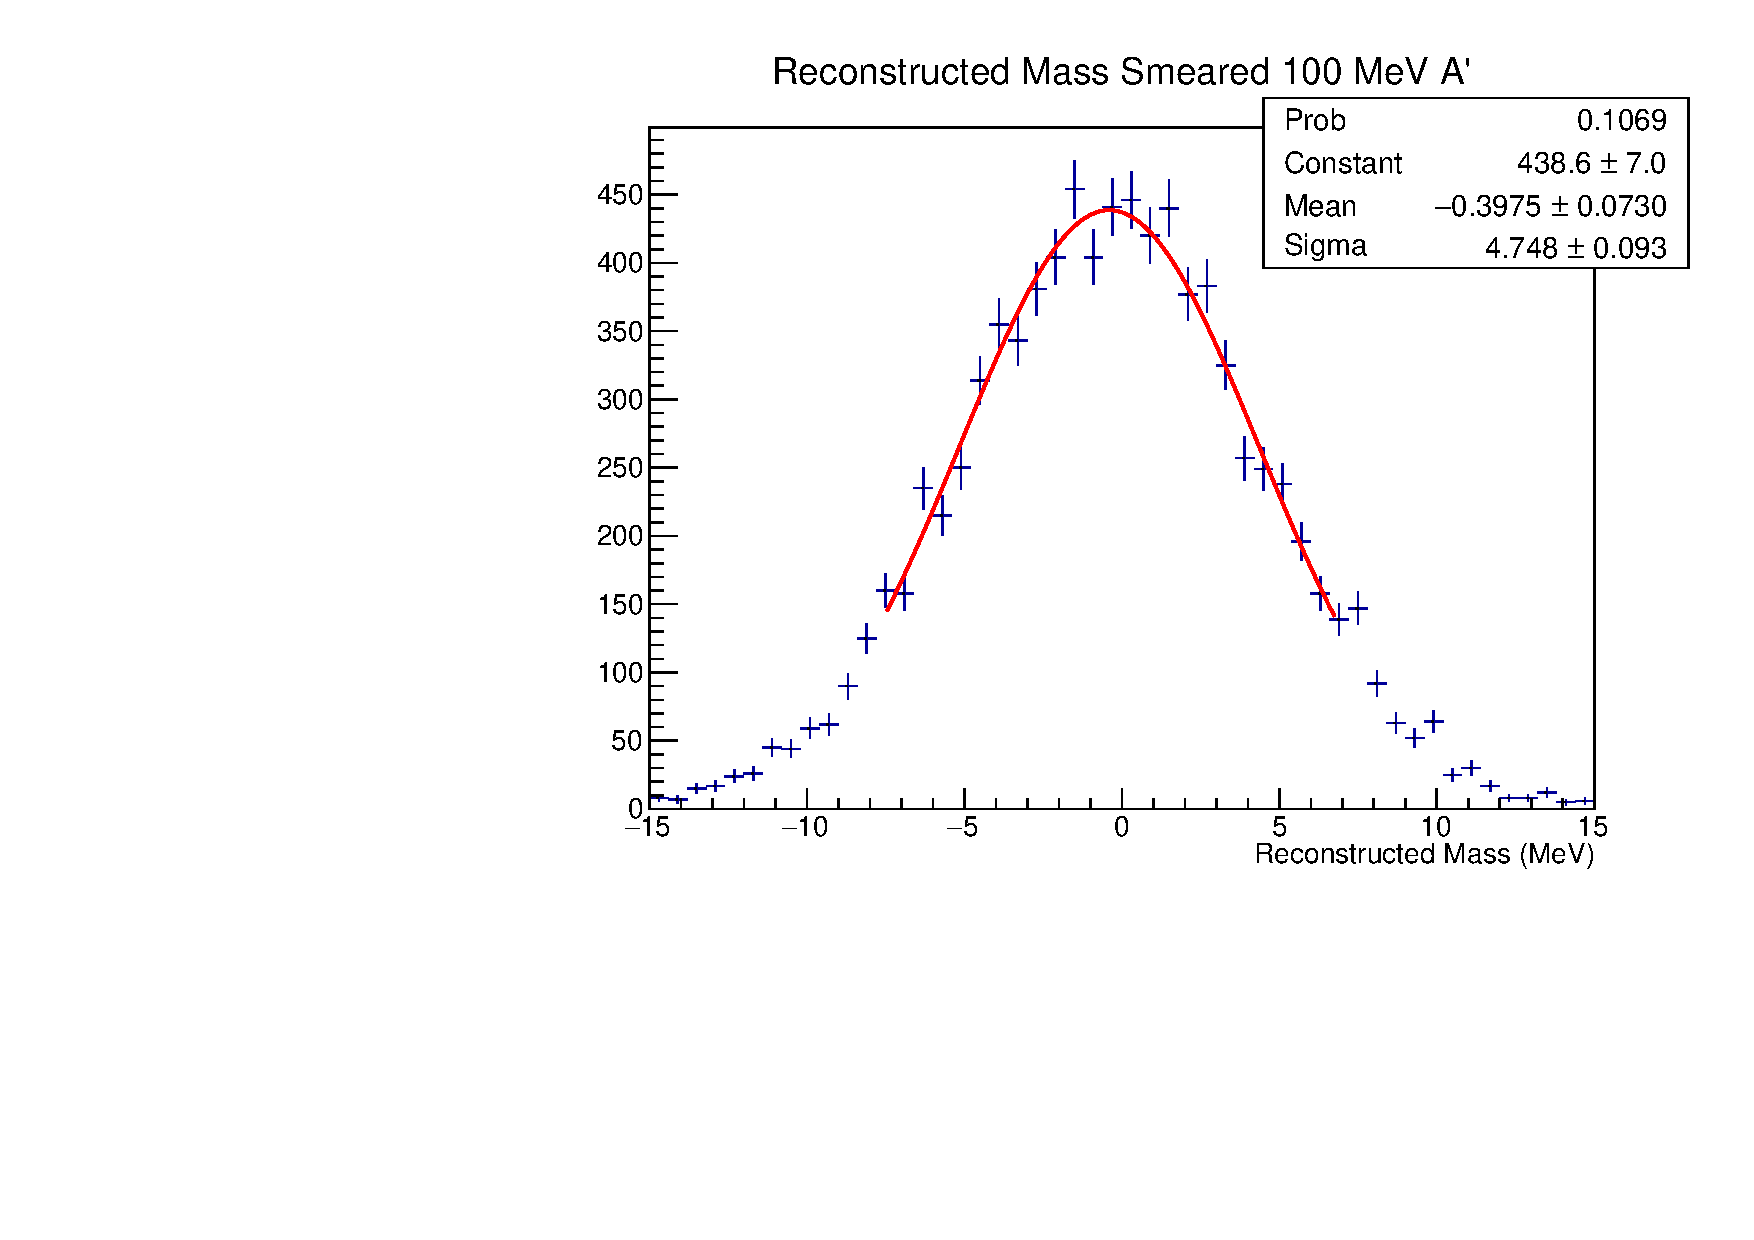
\includegraphics[width=.45\textwidth]{figs/selection/massResL1L2_ap100MeV_smeared.pdf}
%    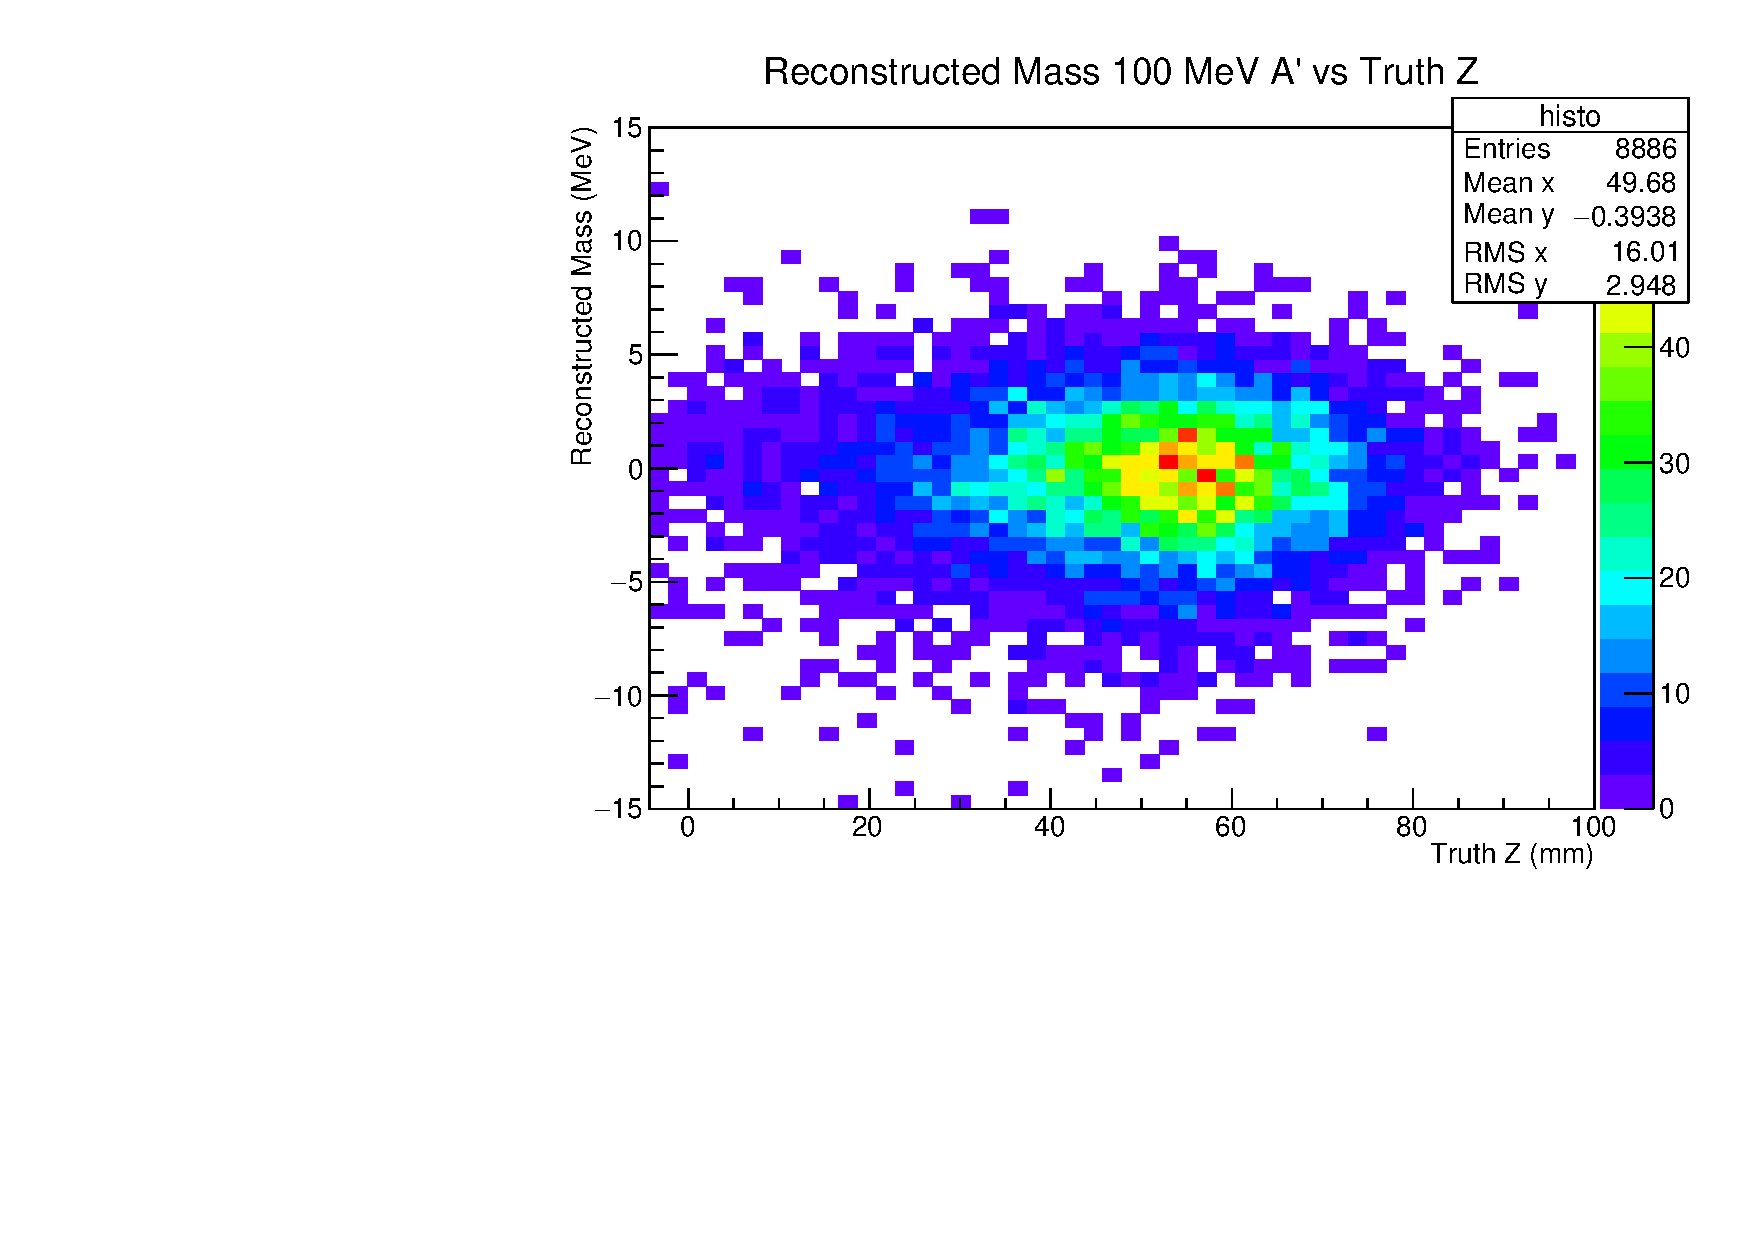
\includegraphics[width=.45\textwidth]{figs/selection/massResL1L2_ap100MeV_m_z.pdf}
%    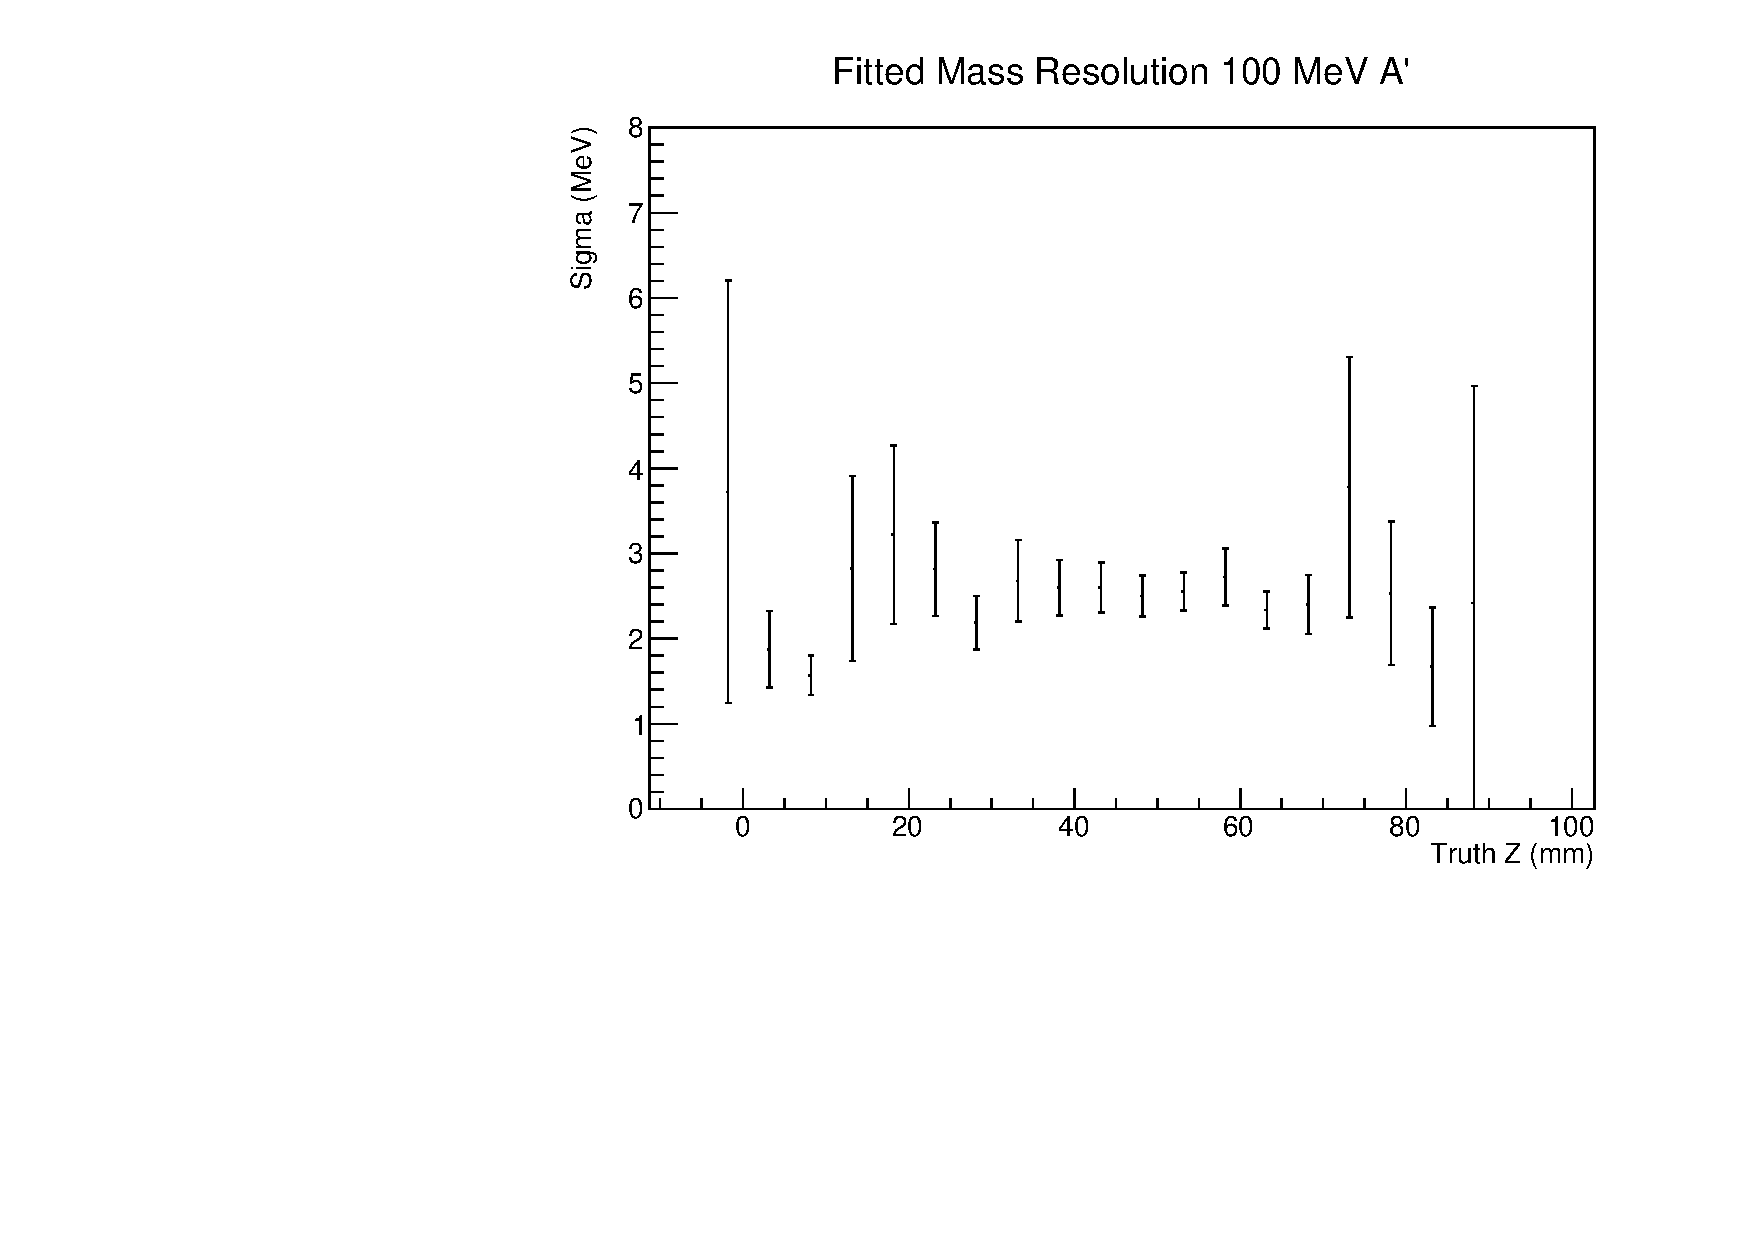
\includegraphics[width=.45\textwidth]{figs/selection/massResL1L2_ap100MeV_z.pdf}
%    \caption{Upper Left: Fitted reconstructed mass spectrum for a 100 MeV displaced $\aprime$. Upper Right: Fitted reconstructed mass spectrum for a 100 MeV displaced $\aprime$ with track momentum smearing. Lower Left: Reconstructed mass vs truth $z$ decay for a 100 MeV displaced $\aprime$. Lower Right: The fitted mass resolution for 100 MeV displaced $\aprime$s as in slices of truth $z$. Mass resolution is approximately independent of decay length. These plots are for the L1L2 category.
%    }
%    \label{fig:mass_resolution_L1L2}
%\end{figure}

\begin{figure}[!hb]
    \centering
    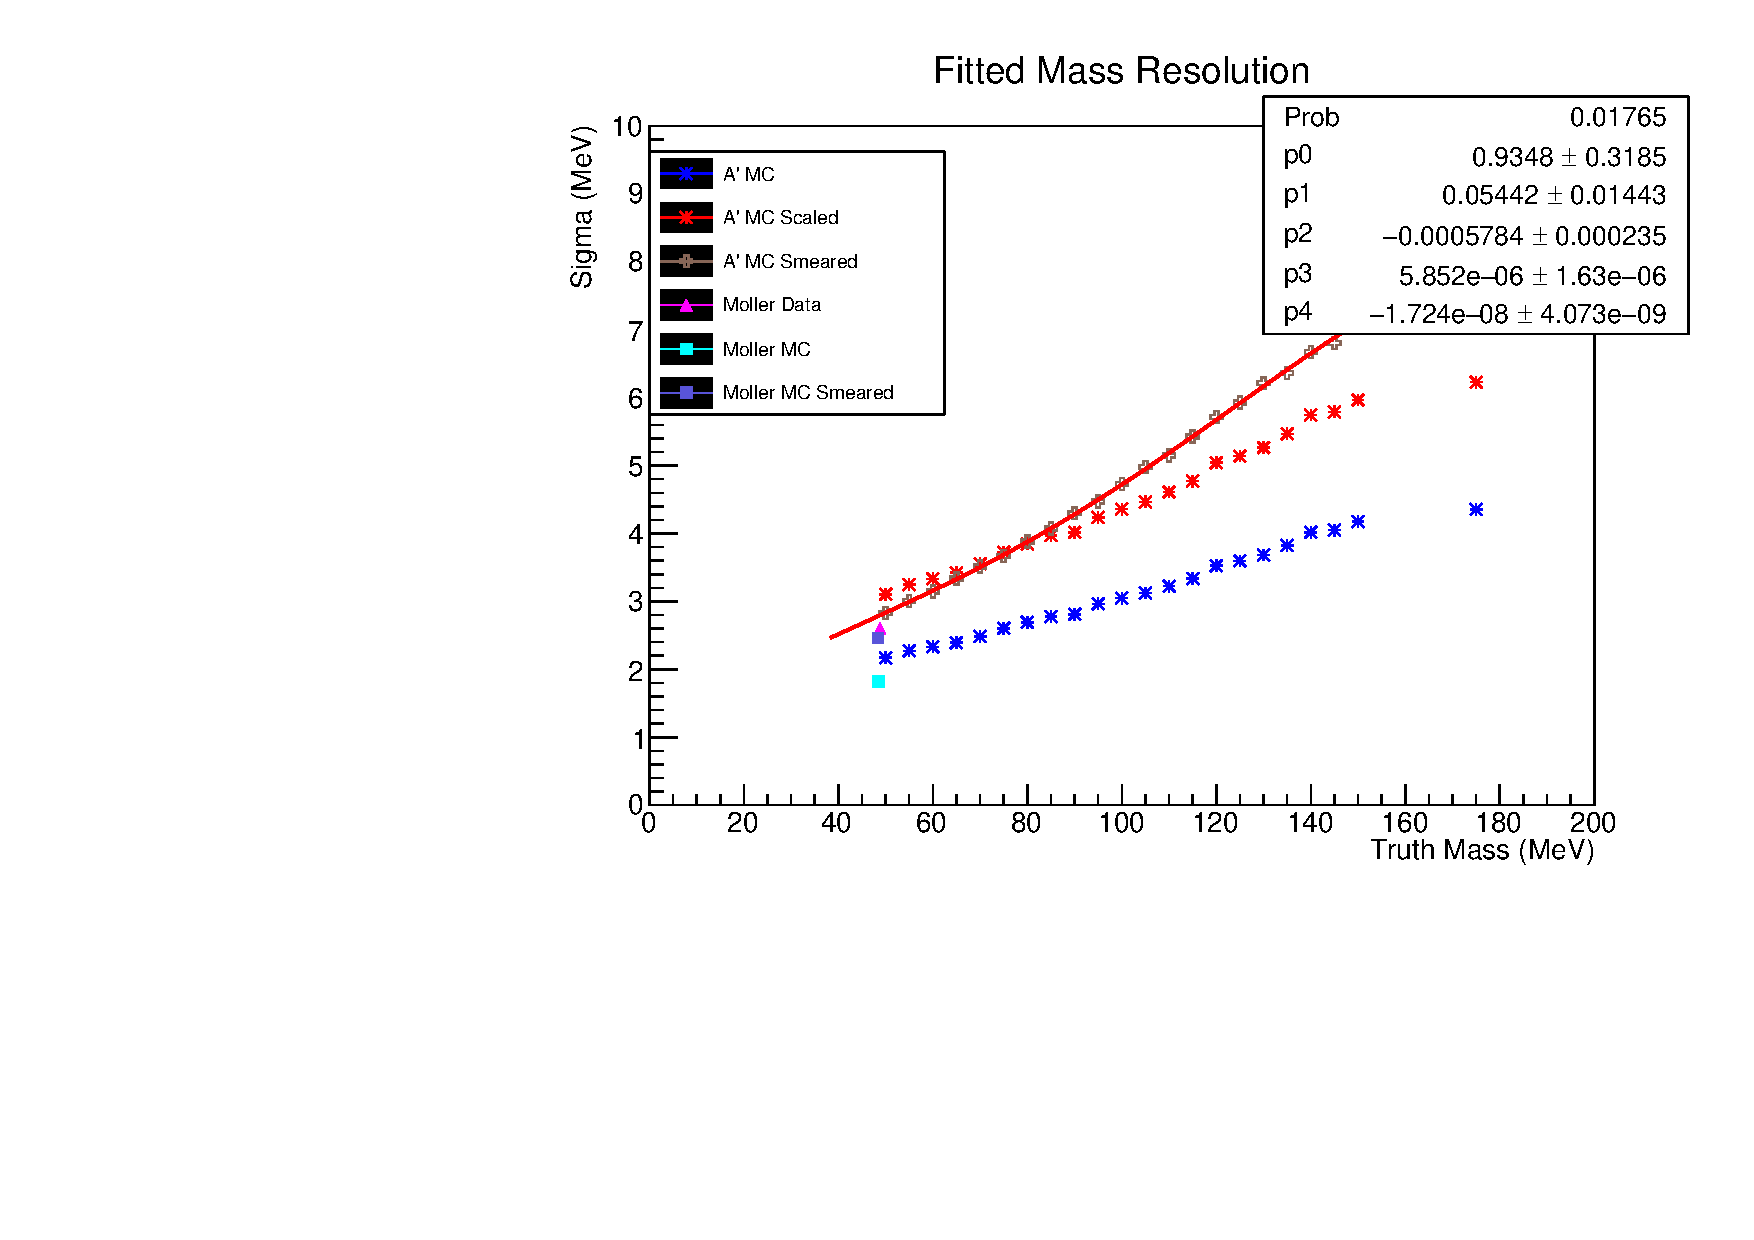
\includegraphics[width=.45\textwidth]{figs/selection/massResL1L1.pdf}
    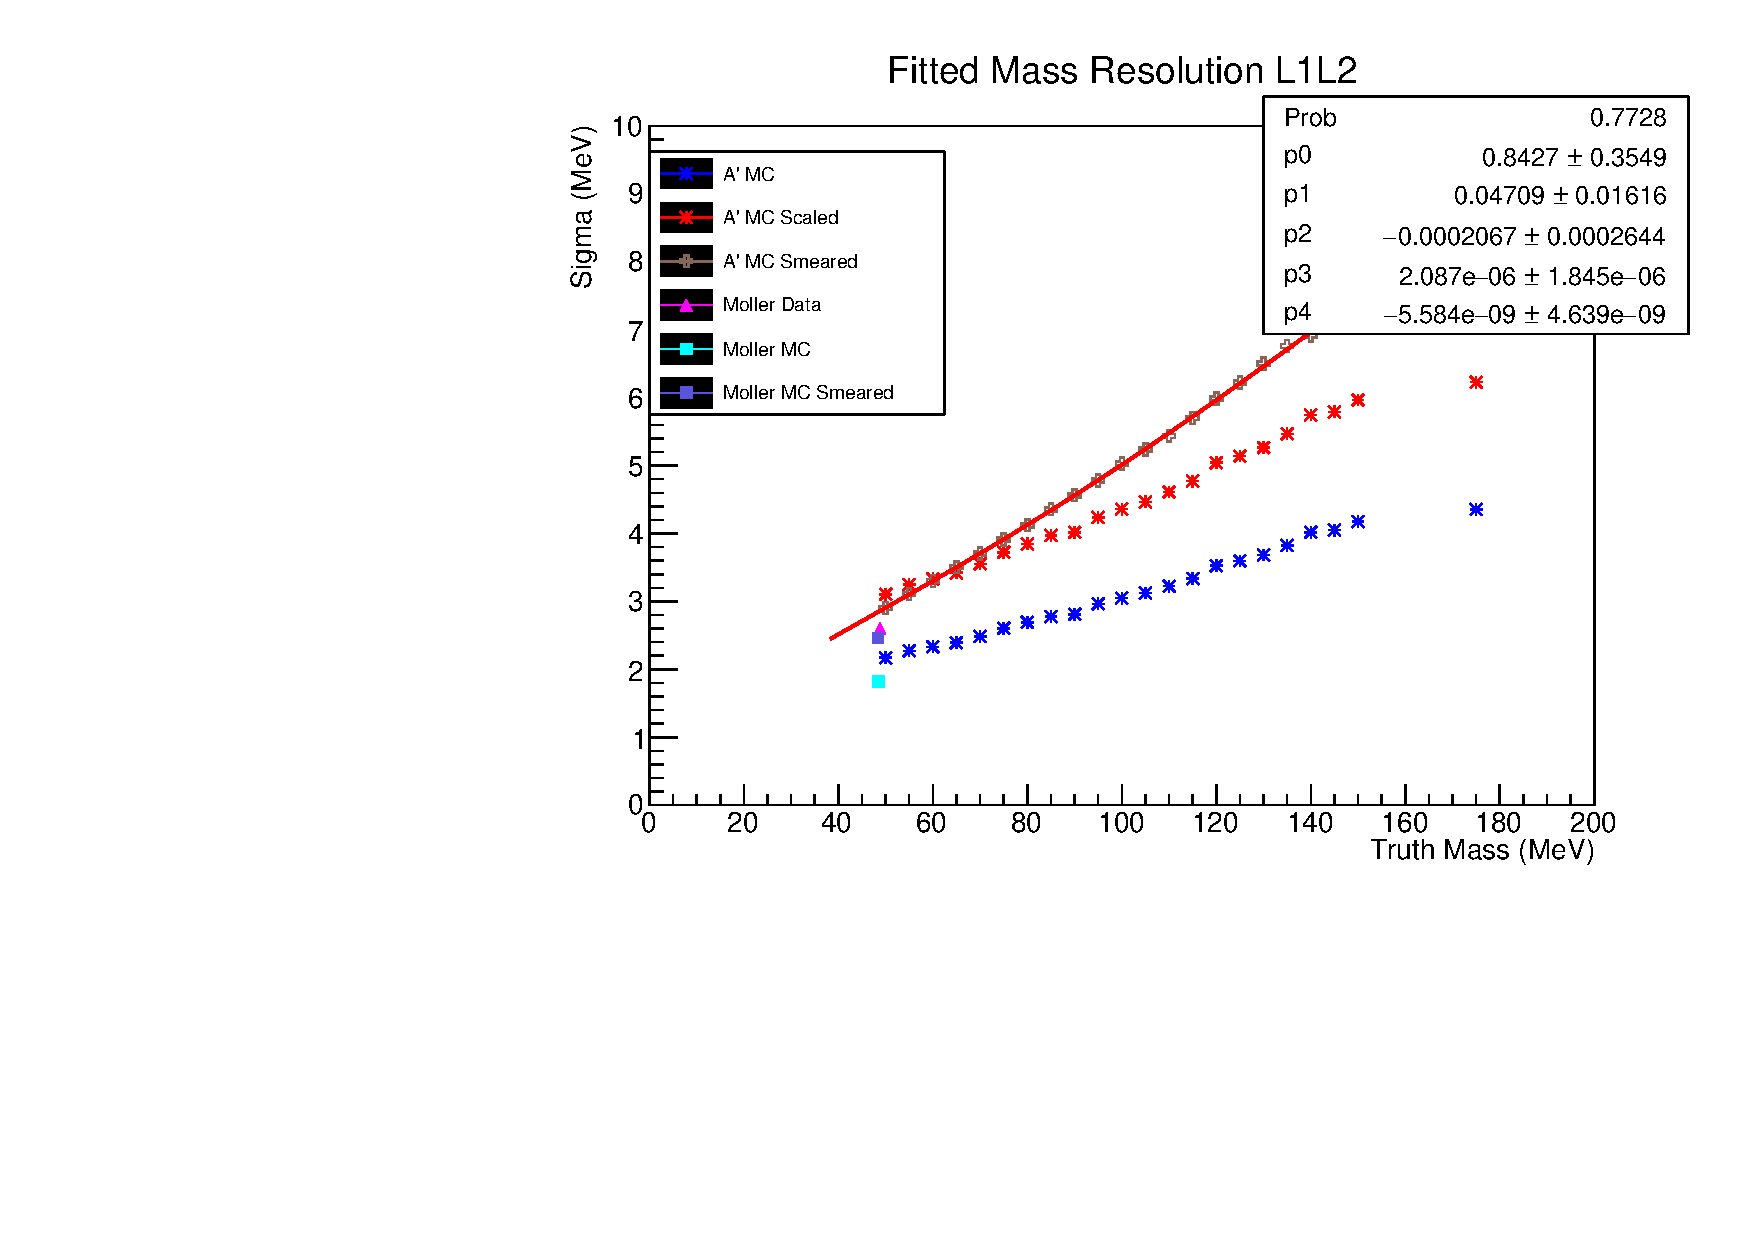
\includegraphics[width=.45\textwidth]{figs/Results/massRes_L1L2.pdf}
    \caption{$\aprime$ mass resolution as a function of mass comparing $\aprime$ MC, $\aprime$ MC scaled using the ratio of the M\o ller mass resolution in data to MC, and $\aprime$ MC with smearing for the Left: L1L1 category and Right: the L1L2 category. The mass resolution is fitted to a 4th order polynomial to the MC with track momenta smearing and is used as an input to the size of the mass bins in the final results.
    }
    \label{fig:mass_resolution}
\end{figure}

\clearpage

\section{Displaced $\aprime$ Rates}\label{sec:aprimerate}

%\section{Displaced A' Rates} \label{sec:aprimes}

The process of computing the expected number of radiative events was shown in Sec. \ref{sec:radfrac} as the product of the radiative fraction $f_{rad}$ and the number of e+e- events in a given narrow mass bin $N_{bin}$. From there, the number of expected $\aprime$s as a function of mass and $\epsilon$ was easily computed by Eq. \ref{eqn:signal_prod} and shown in Fig. \ref{fig:ap_yield}. From the production rate of $\aprime$s at the target, which has the same event selection as Table \ref{tab:radfrac}, the next step is to consider the effects of livetime (for particular choices of $\aprime$ mass and $\epsilon^2$) and the geometrical acceptance to determine the expected signal sizes for long-lived $\aprime$s.% displace the $\aprime$s as a function of $m_{\aprime}$ and $\epsilon$ and do the proper accounting for geometrical acceptance effects.

%\begin{equation}
%S(m_{A'},\epsilon)=f_{rad} N_{bin} \frac{3\pi \epsilon^2}{2N_{eff} \alpha} \frac{m_{A'}}{\delta m_{A'}} 
%    \label{eqn:signal_prod}
%\end{equation}

%where $N_{eff}$ is the number of possible A' decay channels (1 for the parameter space of interest) and $\delta m_{A'}$ is the narrow mass bin width of width 1 MeV. Now that we have the production rate, we must do the proper accounting for the fact that the parameter space of interest for the displaced vertex search are actually downstream decays.

\subsection{$\aprime$ Acceptance Effects}\label{sec:acceptance}

\begin{figure}[t]
    \centering
    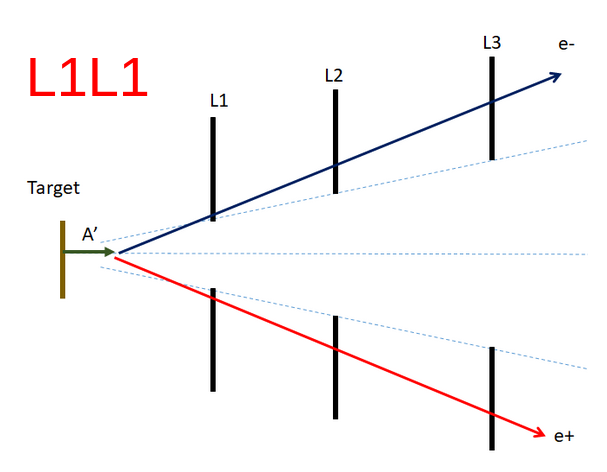
\includegraphics[width=.45\textwidth]{figs/selection/L1L1_schem.png}
    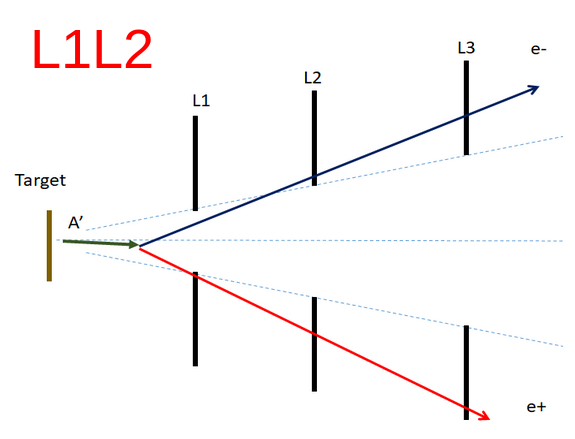
\includegraphics[width=.45\textwidth]{figs/selection/L1L2_schem.png}
    \caption{Left: Schematic of a relatively short $A'$ decay length in which both daughter particles have a layer 1 hit. This is referred to as L1L1. Right: Schematic of a relatively long $A'$ decay length in which one of the daughter particles misses layer 1 (but hits layer 2) and the other daughter particle hits layer 1. This is referred to as L1L2.}
    \label{fig:L1L2_L1L2_schem}
\end{figure}

The SVT is designed to have a geometrical acceptance of 15 mrad for prompt decays. However, downstream decays must have a larger opening angle to remain in the acceptance of the SVT, and the further downstream the decay, the more likely the daughter particles will miss the SVT. Thus, the geometrical acceptance drops dramatically with increasing decay length. Based on geometrical acceptance and $\aprime$ decay kinematics, there are several possibilities for a long-lived $\aprime$.
\begin{enumerate}
  \item The $\aprime$ has a finite, but relatively short decay length, and both of the $\aprime$ daughter particles have layer 1 hits in the SVT. This category is denoted as L1L1 (where the 1's denote the first layer of the SVT that the $\aprime$ daughter particles hit).
  \item The $\aprime$ has a slightly longer decay length than those that fall into the L1L1 category causing exactly one of the $\aprime$ daughter particles to miss layer 1 but hit layer 2, whereas the other particle hits layer 1. This category is denoted as L1L2.
  \item The $\aprime$ has a longer decay length than the L1L2 category causing both of the $\aprime$ daughter particles to miss layer 1, but both particles have hits in layer 2. This category is denoted as L2L2.
  \item The $\aprime$ has a relatively long decay length or a small opening angle where at least one of the $\aprime$ daughters misses both layer 1 or layer 2. In these cases, the $\aprime$ is not reconstructed since track reconstruction requires a minimum of five 3-D hits.
\end{enumerate}

\begin{figure}[t]
    \centering
    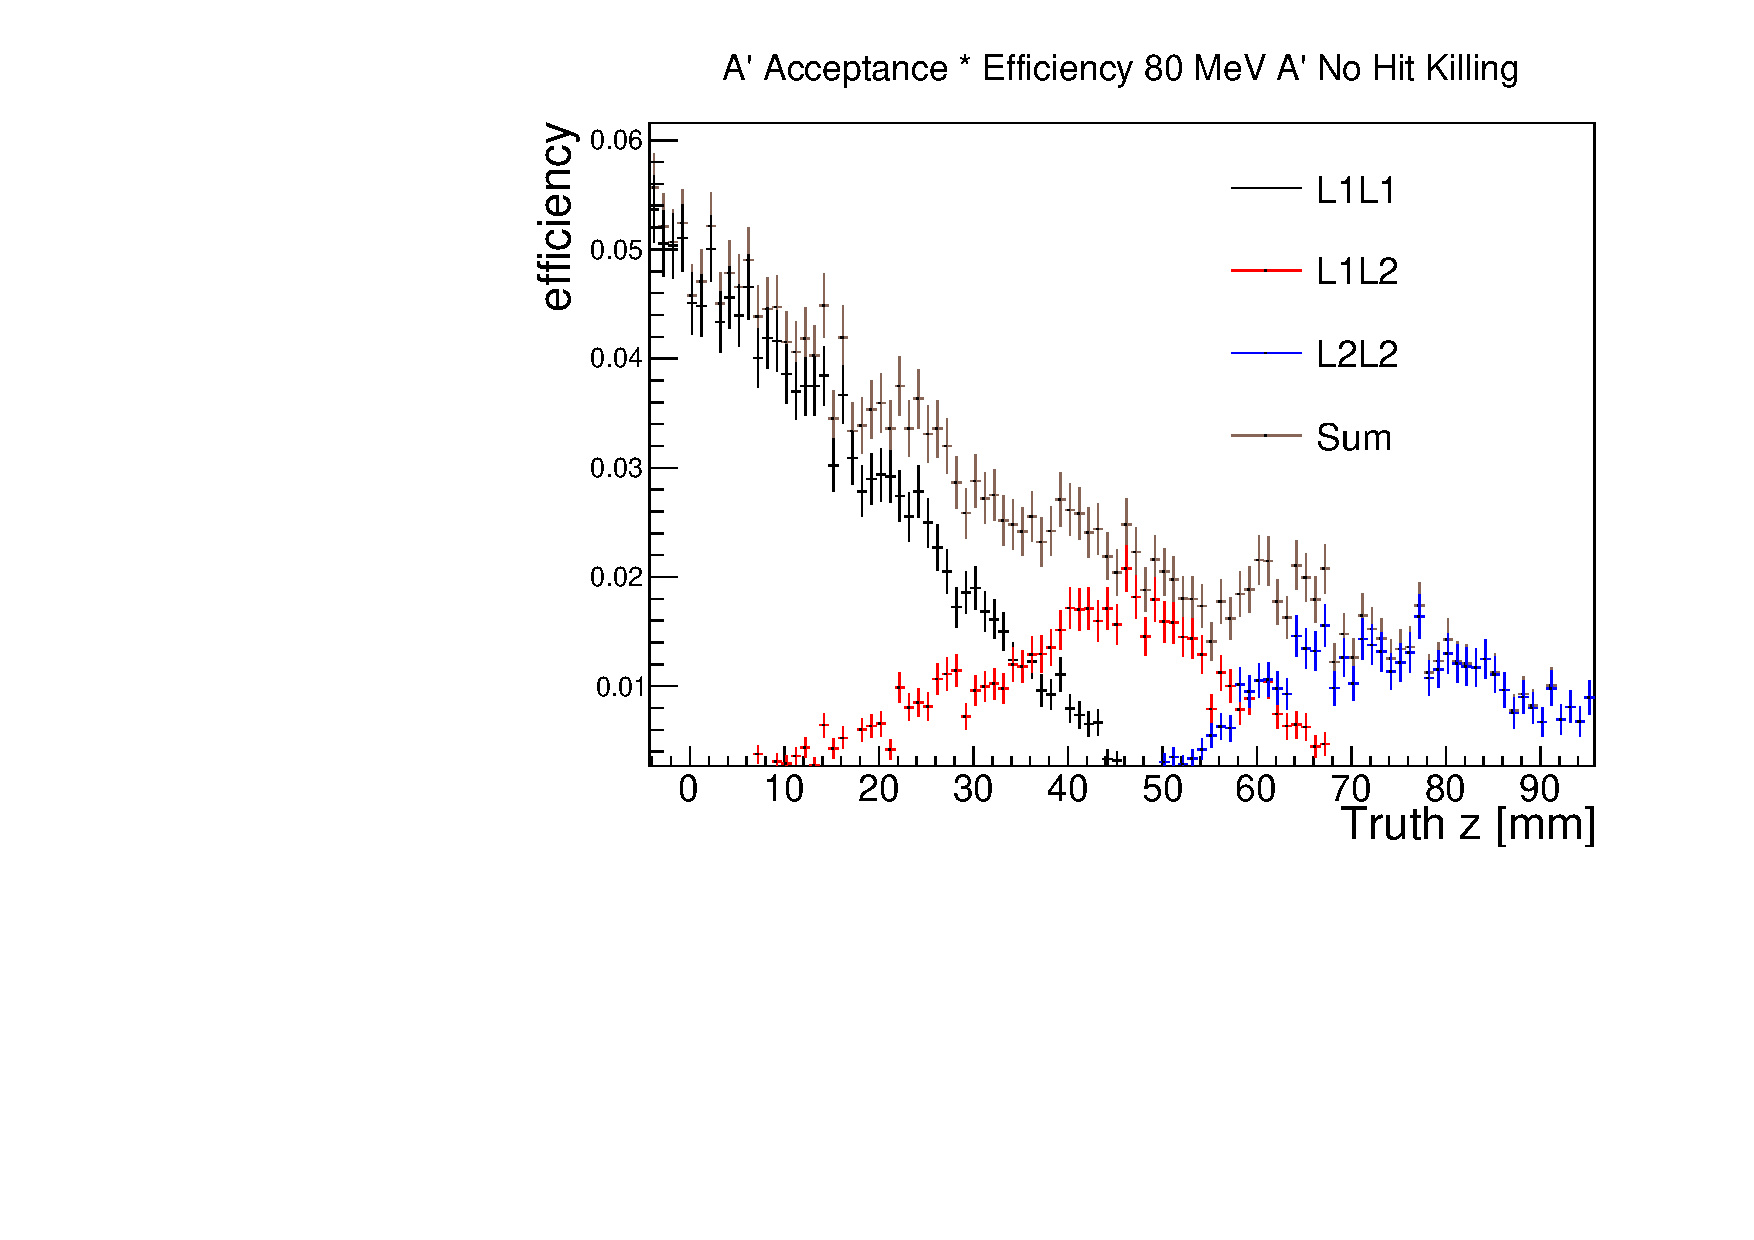
\includegraphics[width=.45\textwidth]{figs/selection/ap_eff_80MeV_nohitkill.pdf}
    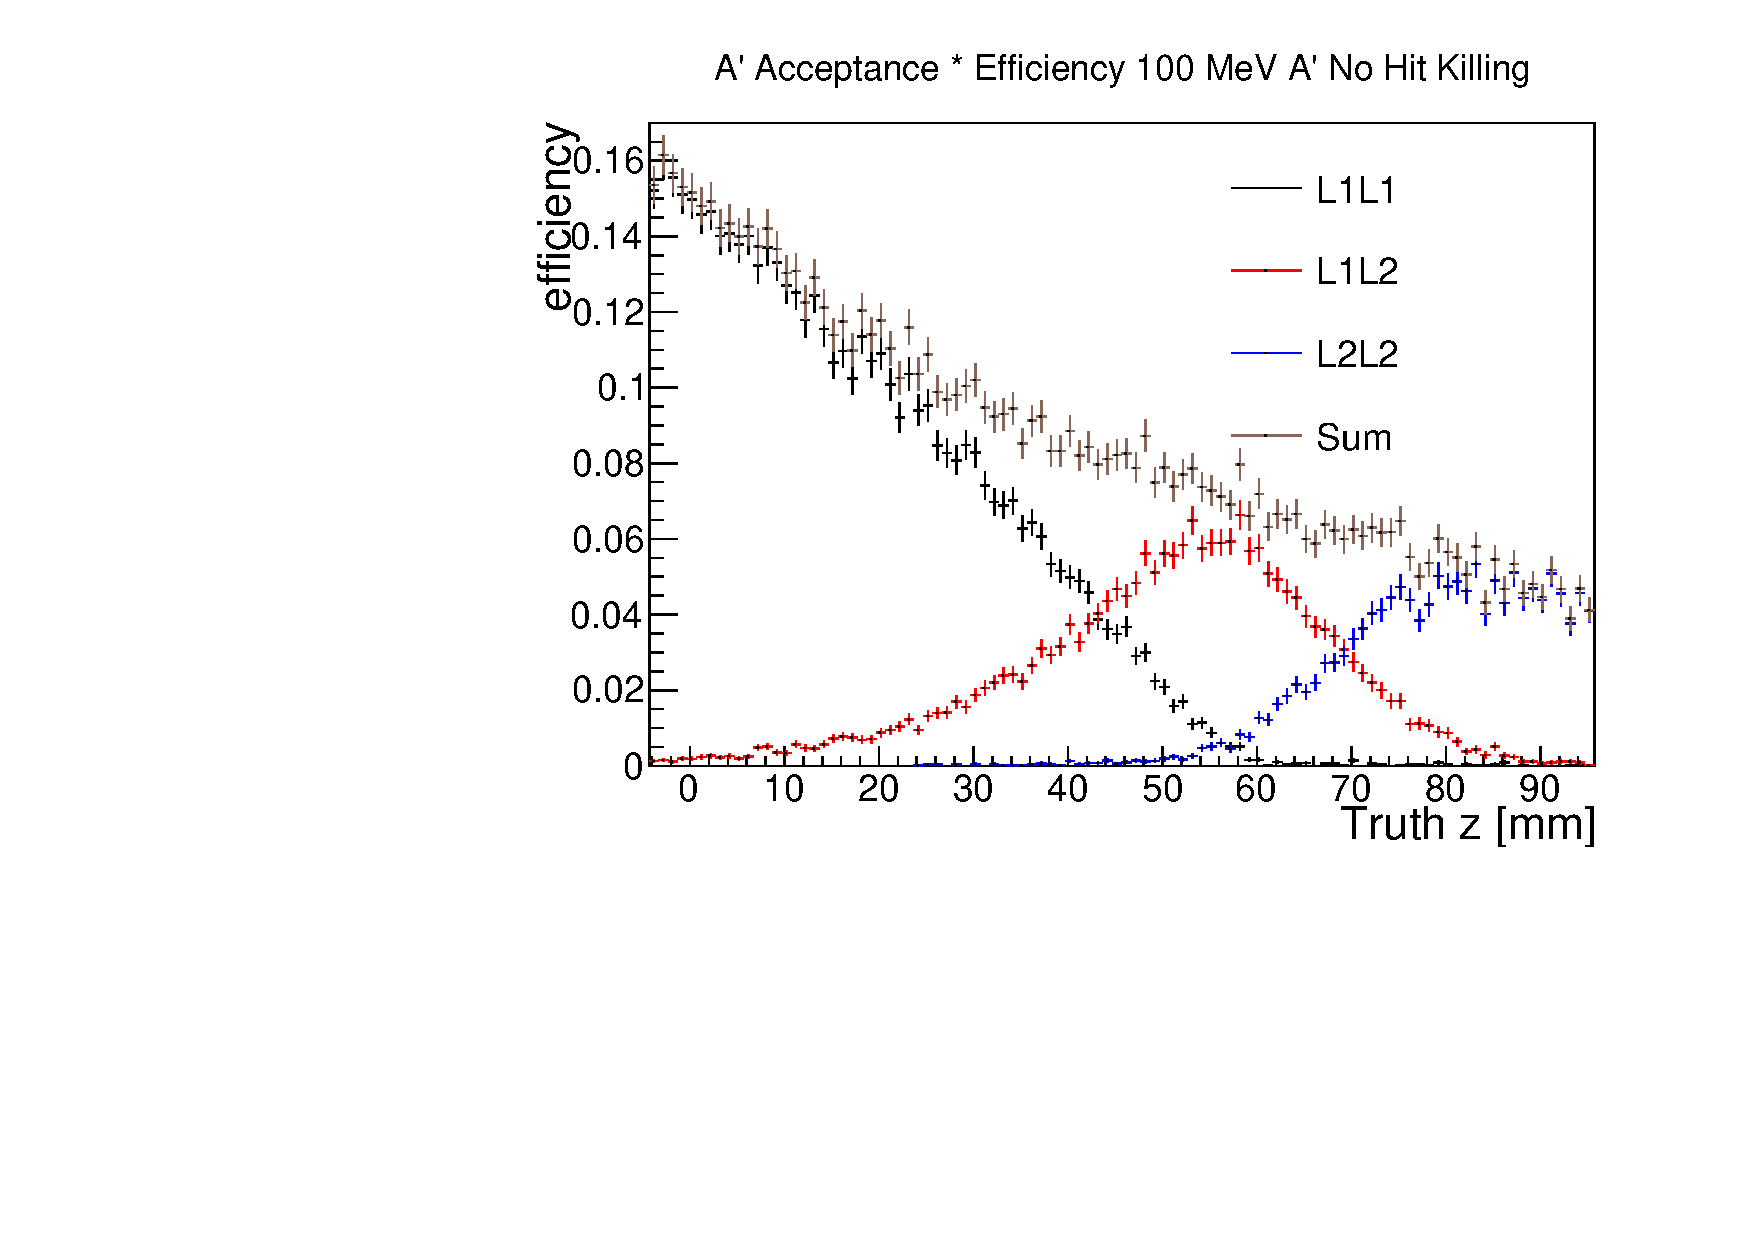
\includegraphics[width=.45\textwidth]{figs/selection/ap_eff_100MeV_nohitkill.pdf}
    \caption{The product of geometrical acceptance and efficiency for displaced $A'$s for the L1L1, L1L2, and L2L2 categories as well as their sum for Left: 80 MeV displaced $\aprime$s and Right: 100 MeV displaced $\aprime$s are on the right.}
    \label{fig:eff_nohitkill}
\end{figure}

Since 5 hits on every track are required, these four mutually exclusive categories are the only viable possibilities. A schematic of the L1L1 and L1L2 categories is shown in Fig. \ref{fig:L1L2_L1L2_schem} and the efficiency as a function the truth $z$ decay position is shown in Fig. \ref{fig:eff_nohitkill}. %The product of the geometrical acceptances and efficiencies of the three categories in which HPS can detect $\aprime$s (L1L1, L1L2, L2L2) as well as their sum is shown in Fig. \ref{fig:eff1}. 
Once the displaced $\aprime$s are placed in the correct category and the geometrical acceptances are properly incorporated, the last step is to properly account for hit efficiencies in the SVT. For instance, hit efficiency effects can cause an $\aprime$ event that should fall into the L1L1 category based on geometrical acceptance to have a missing layer 1 hit due to an inefficiency. This example would cause the $\aprime$ event to migrate into L1L2 category. Unfortunately, the hit efficiencies are not properly accounted for in the MC and their study is ongoing. However, as a quick post-reconstruction fix, a hit killing method is implemented and described in the following subsection in Sec. \ref{sec:hitkill}. %and the remaining event selections (isolation cut, impact parameter cut, and V0 extrapolation to the target cut) for each of the individual categories. The hit killing method and algorithm are described in the following subsection in Sec. \ref{sec:hitkill}. %Of the A's that remain in one of the three categories based on geometric acceptance, there are several things that can happen:

%\begin{enumerate}
%  \item Both tracks pass the hit killing algorithm and passes remaining cuts. The event remains in its respective L1L1, L1L2, or L2L2 category.
%  \item In the L1L1 category, exactly one of the tracks fails the hit killing algorithm. If this track has 6 hits, the event migrates into the L1L2 category.
%  \item In the L1L1 category, both of the tracks fail the hit killing algorithm. If these tracks both have 6 hits, the event migrates into the L2L2 category.
%  \item In the L1L1 category, one or both of the tracks fails the hit killing algorithm. If at least one of the tracks that fails the hit killing has 5 hits, the event is eliminated.
%  \item In the L1L2 category, the track with a layer 1 hit fails the hit killing algorithm. If this track has 6 hits, the event migrates into the L2L2 category. The hit killing algorithm is not applied to the track without the layer 1 hit since it's only applied to layer 1.
%  \item In the L1L2 category, the track with a layer 1 hit fails the hit killing algorithm. If this track has 5 hits, the event is eliminated.
%  \item In the L2L2 category, events remain untouched since the hit killing algorithm is only applied to layer 1.
%\end{enumerate}

%After the hit killing algorithm is applied, the remaining cuts in each category are applied separately as in Sec. \ref{sec:selection} followed by the selection of events with only a single V0 particle remaining.

\clearpage

\subsection{Hit Killing}\label{sec:hitkill}
The HPS detector has hit efficiency effects, particularly in the first layer of the SVT,  as described in Sec. \ref{sec:hiteff} that must be accounted for in the $\aprime$ MC in order to properly normalize the expected signal rate. Hit efficiencies are measured as a function of channel number in the SVT, and although the eventual goal is to implement a hit killing algorithm based on channel number, a simple post-reconstruction hit killing algorithm based on track slope (tan$\lambda$) is implemented. The layer 1 efficiency used as a function of track slope is shown in Fig. \ref{fig:L1_eff}. Since the hit efficiency in the other layers is $>99$\%, the hit killing algorithm is only applied to layer 1 hits. %Hit efficiencies are measured using a track refit to a layer of interest, and an unbiased extrapolation to the layer to see if a hit lies withing a certain window. %A sample of measured hit efficiency in data in comparison with MC for the layer 1 bottom stereo sensor is shown in Fig. \ref{fig:L1_eff}. 

\begin{figure}[t]
    \centering
    %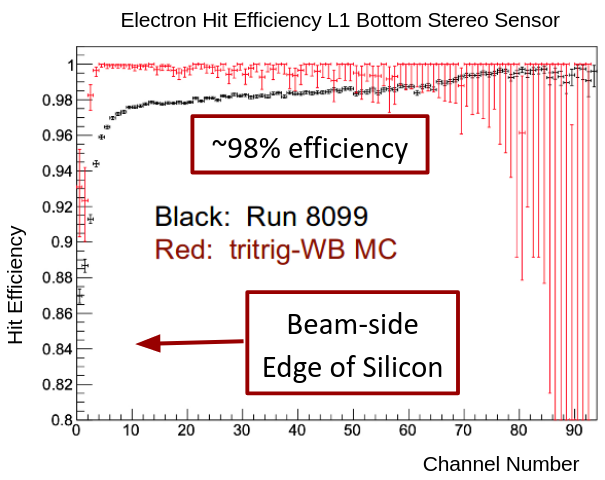
\includegraphics[width=.45\textwidth]{figs/recon/hiteff.png}
    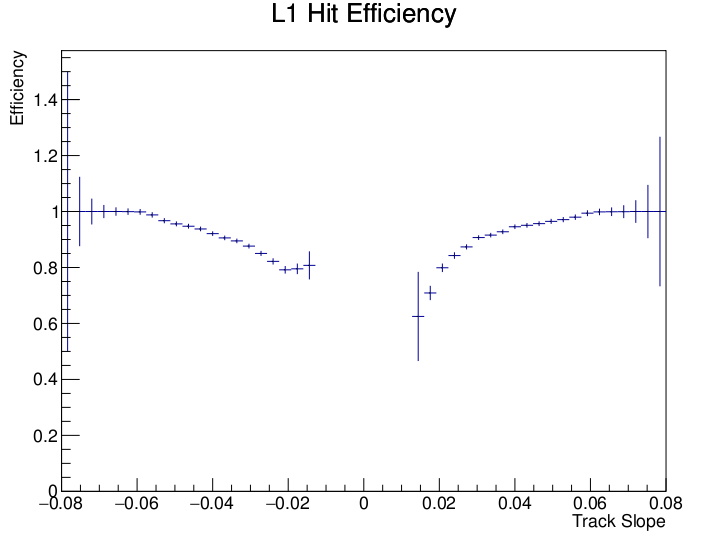
\includegraphics[width=.45\textwidth]{figs/recon/L1_eff.png}
    \caption{%Left: The measured SVT layer 1 efficiency for electrons in layer 1 bottom stereo sensor. The MC does not have the correct hit efficiencies. Right: 
    The layer 1 efficiency used for the hit killing algorithm as a function of track slope (tan$\lambda$). There is a small top/bottom asymmetry, part of which can be attributed to increased small angle track acceptance for the bottom hemisphere. The active edge is placed at 1.5 mm in both top and bottom halves; however, the bottom SVT is shifted downstream by $\sim$10 mm resulting in increased acceptance to tracks with smaller tan$\lambda$.}
    \label{fig:L1_eff}
\end{figure}

%Unfortunately hit efficiencies are not present in the MC, although this is on the future agenda. However, this is an effect that will affect the signal rate, particularly in which of the categories the signal lies in. To account for hit efficiencies in a reasonable way, a post-reconstruction hit killing algorithm is applied as a function of track slope shown in in Fig. \ref{fig:L1_eff}. 

If a track passes the hit killing algorithm, nothing changes. However, if a track fails the hit killing algorithm, the layer 1 hit is removed and the $\aprime$ can either migrate into another category or be eliminated. Details on several possibilities of an $\aprime$ event passed through the hit killing algorithm are as follows:

\begin{enumerate}
  \item Begin with the L1L1 category. Based on track slope, decide if each positron and electron track passes the hit efficiency cut. There are 4 possible scenarios.
  \begin{enumerate}
    \item If both pass, the event remains in the L1L1 category. 
    \item If either track fails to pass the cut and had only 5 hits on track, the event is removed. 
    \item If exactly one track fails to pass the cut and had 6 hits on track, the event is moved to the L1L2 category. 
    \item If both tracks fail to pass the cut and both tracks have 6 hits on track, the event is moved to the L2L2 category.
  \end{enumerate}
  \item Next move to the L1L2 category (excluding those events that have migrated into the L1L2 category from the L1L1 category). For this category, since only layer 1 inefficiencies are considered and exactly one track contains a layer 1 hit, only the track with the layer 1 hit is considered. Again based on track slope, decide if the positron or electron track passes the hit efficiency cut. There are 3 possible scenarios.
  \begin{enumerate}
    \item The track with the layer 1 hit passes the hit efficiency cut, it remains in the L1L2 category.
    \item The track with the layer 1 hit fails the hit efficiency cut and has 5 hits on track. This event is removed.
    \item The track with the layer 1 hit fails the hit efficiency cut and has 6 hits on track. This event is moved to the L2L2 category.
  \end{enumerate}
  \item Finally, no events are removed from the L2L2 category since only layer 1 efficiencies are considered and L2L2 events have no layer 1 hit by definition. However, L2L2 gains some of the $\aprime$ events from L1L1 and L1L2 categories. As previously explained, L2L2 is not considered for this analysis.
  \item Lastly, add the events that have migrated from L1L1 into L1L2, and add the events that have migrated from L1L1 and L1L2 into L2L2.
\end{enumerate}

These steps complete the post-reconstruction track slope-dependent hit killing algorithm thus incorporating the efficiency curves for $\aprime$s as a function of $z$ that includes both geometrical acceptance and hit efficiency effects. An example of the efficiency curves divided into the three mutually exclusive categories (and their sum) for two $\aprime$ masses after the hit killing algorithm is shown in Fig. \ref{fig:eff1}.

\begin{figure}[t]
    \centering
    %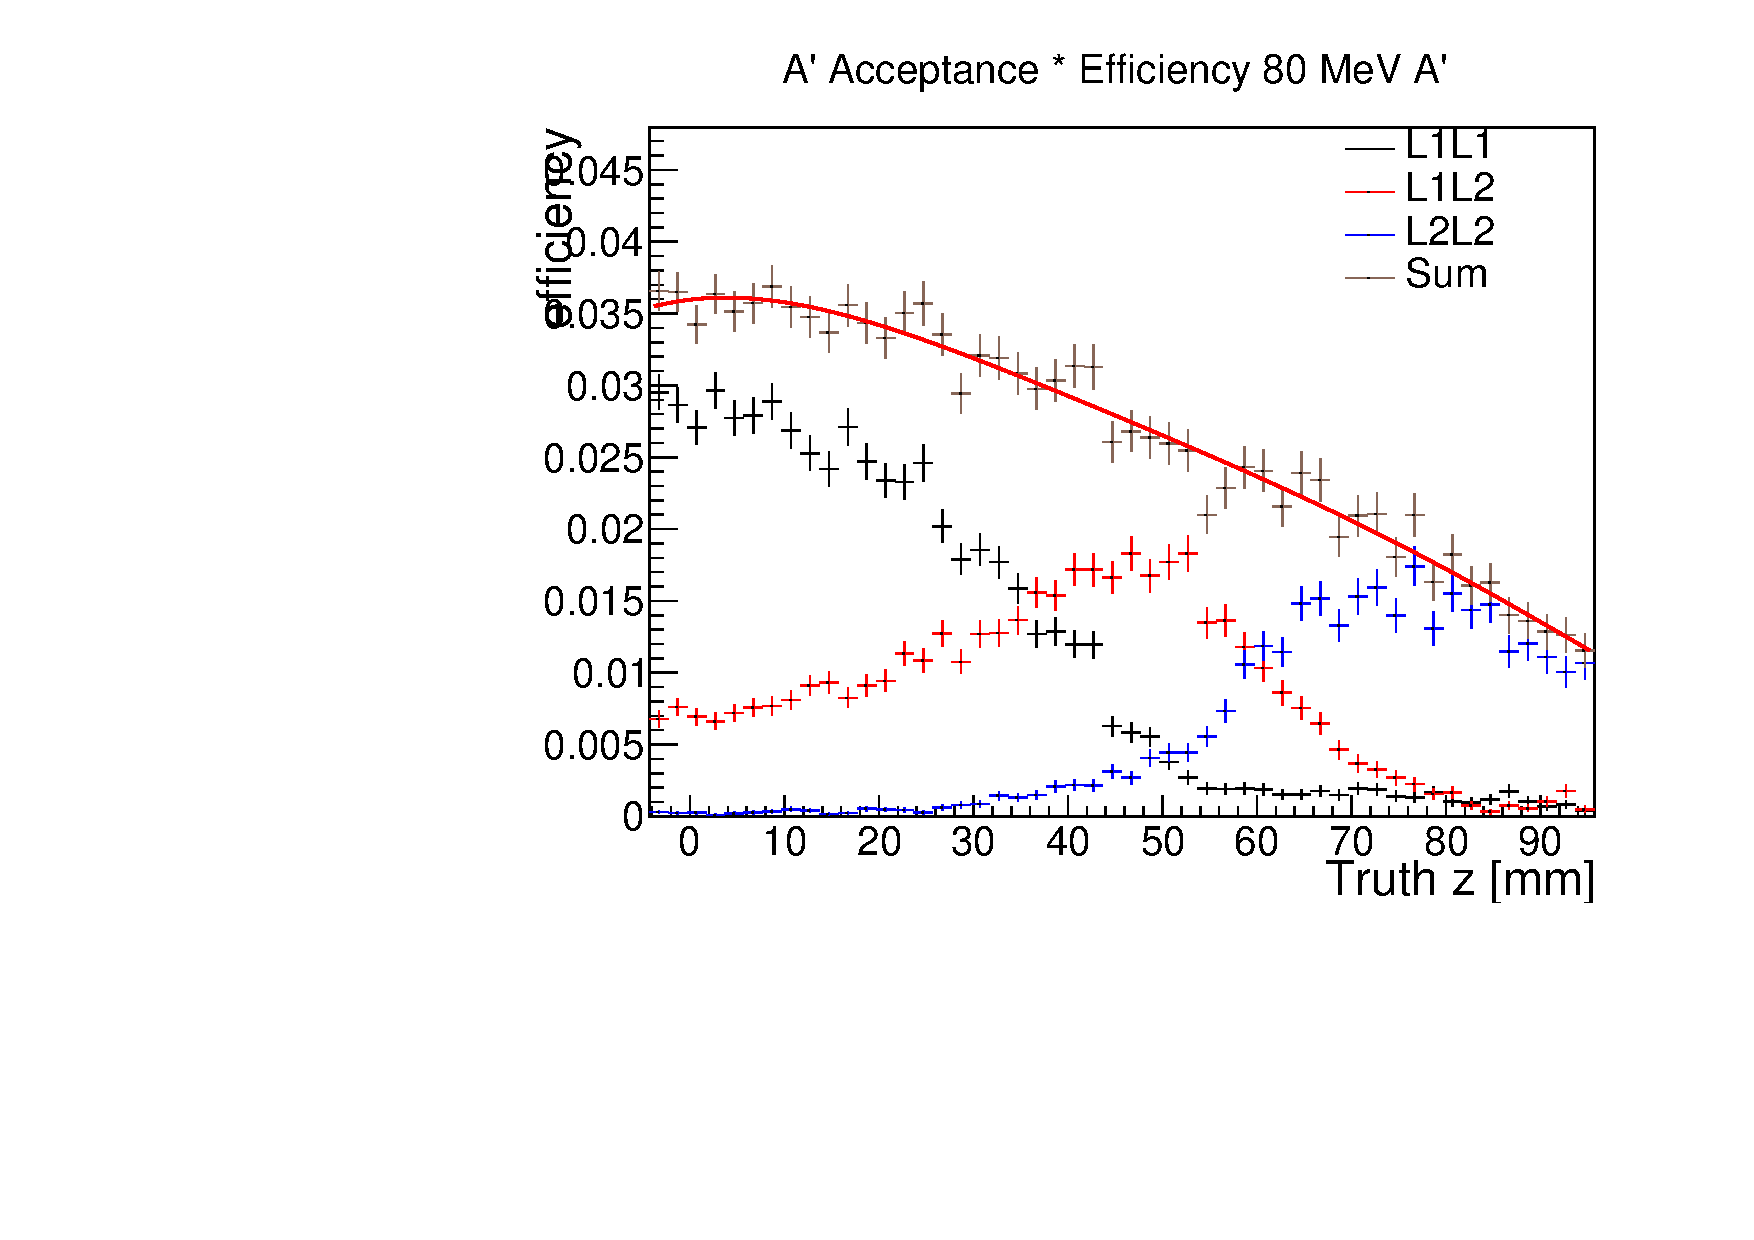
\includegraphics[width=.45\textwidth]{figs/selection/ap_80MeV_eff_fit.pdf}
    %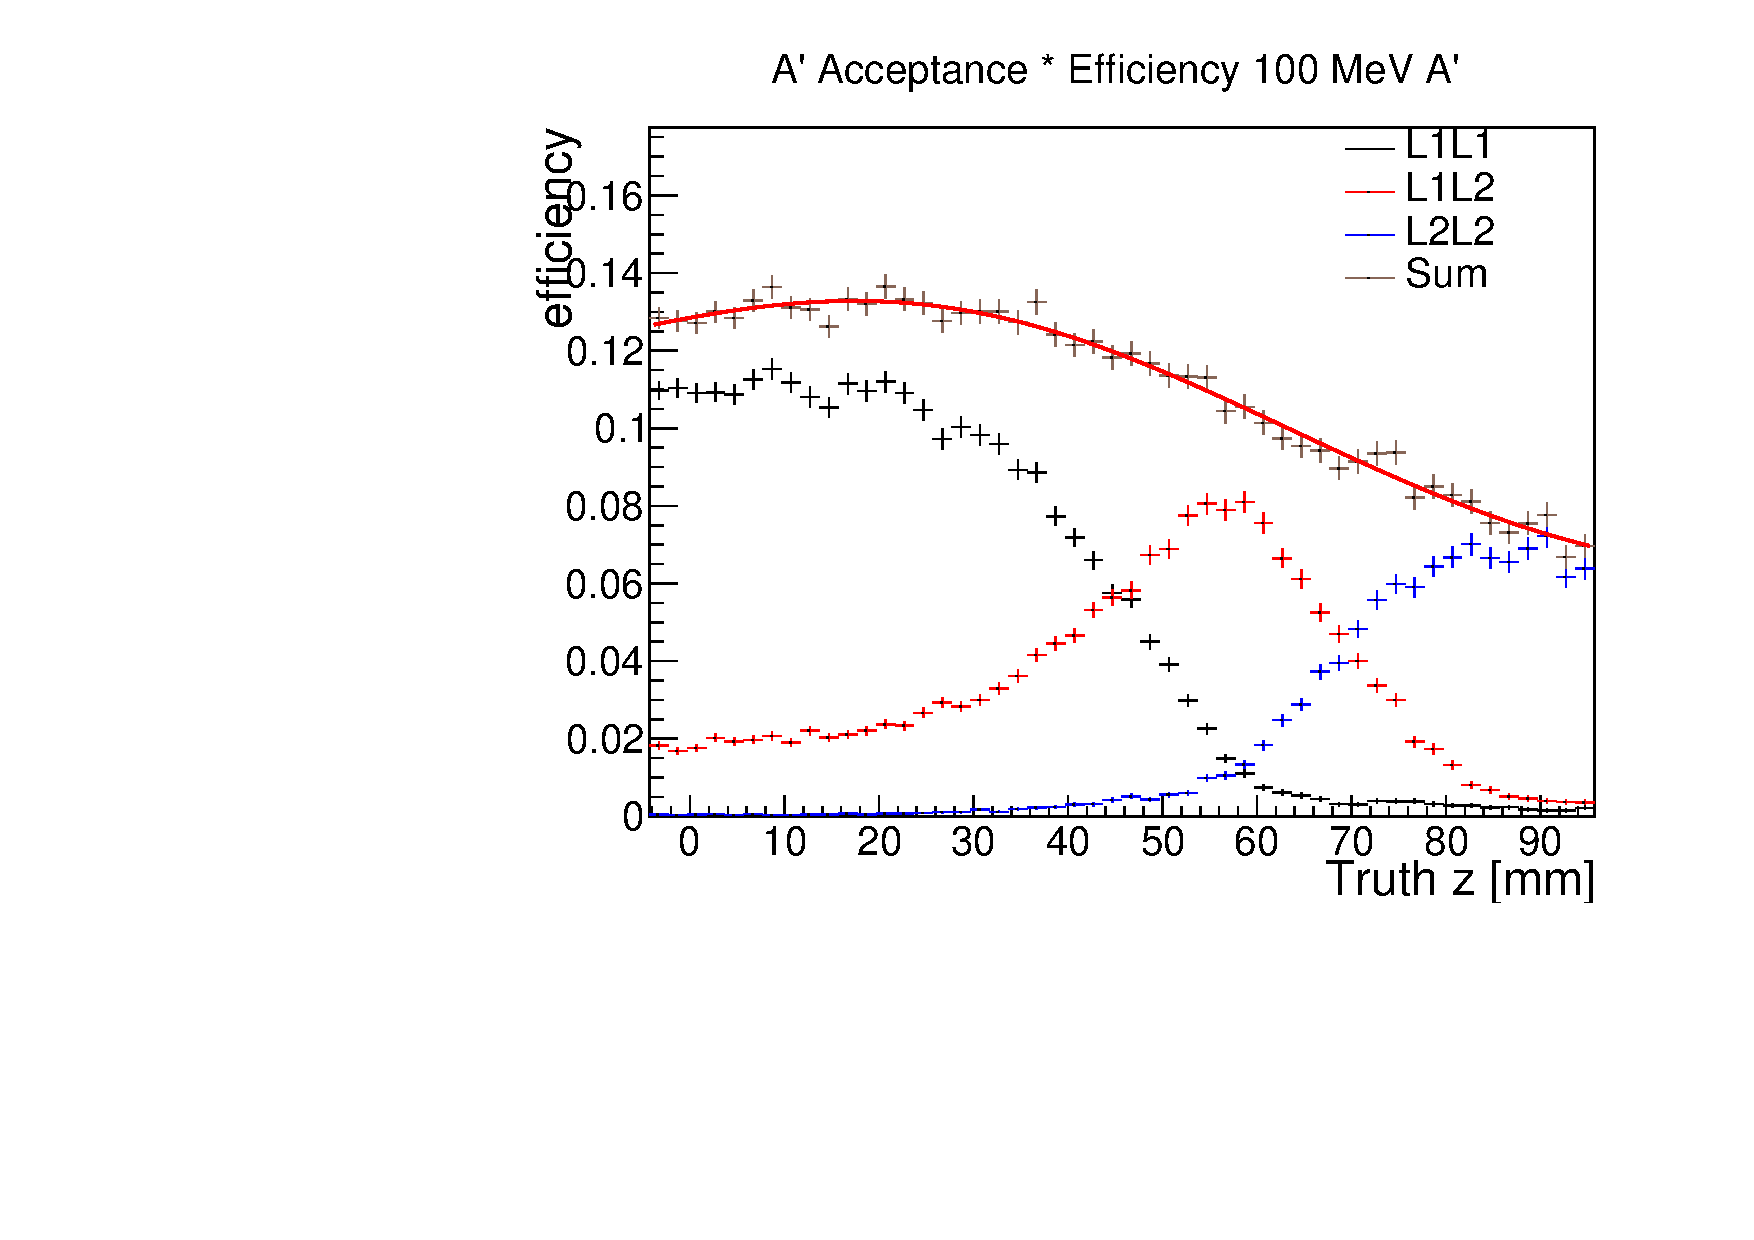
\includegraphics[width=.45\textwidth]{figs/selection/ap_100MeV_eff_fit.pdf}
    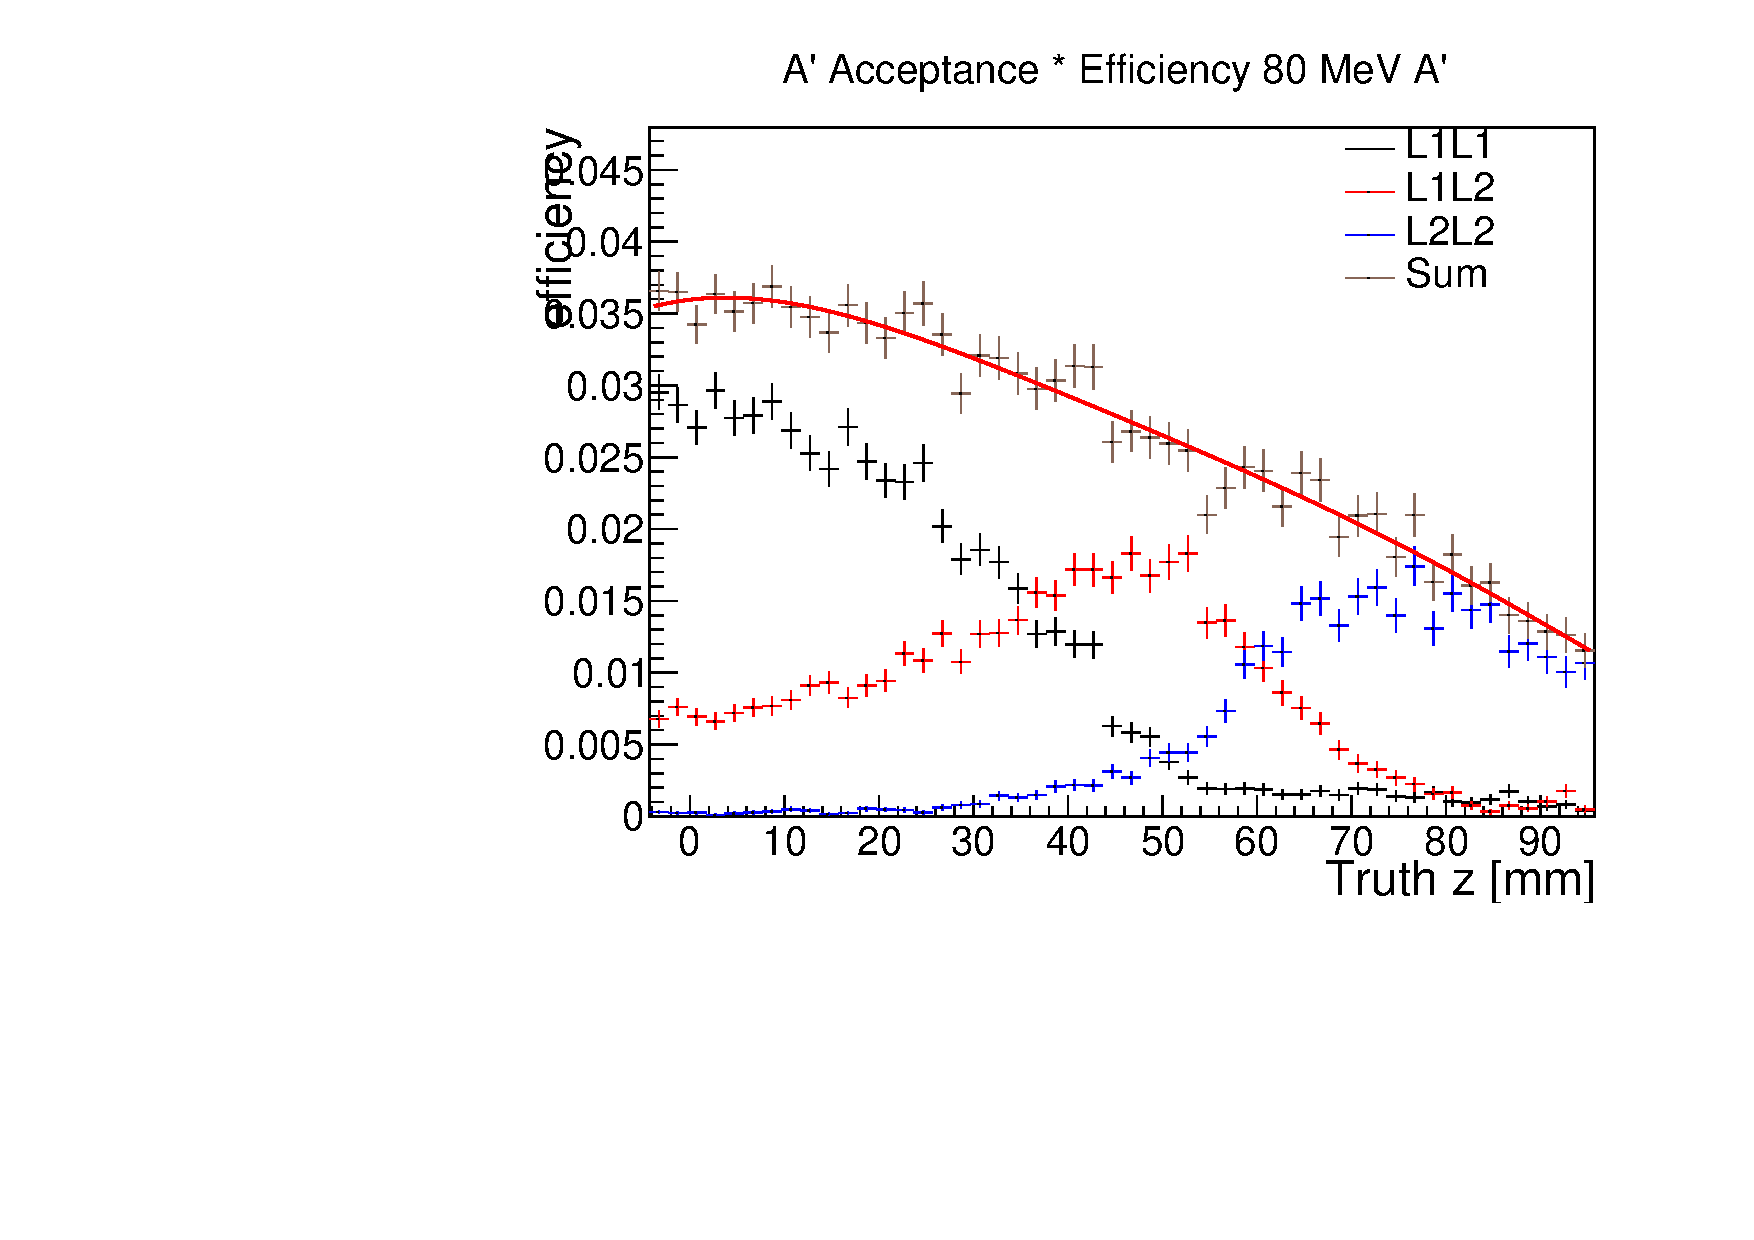
\includegraphics[width=.45\textwidth]{figs/selection/ap_80MeV_eff_fit.pdf}
    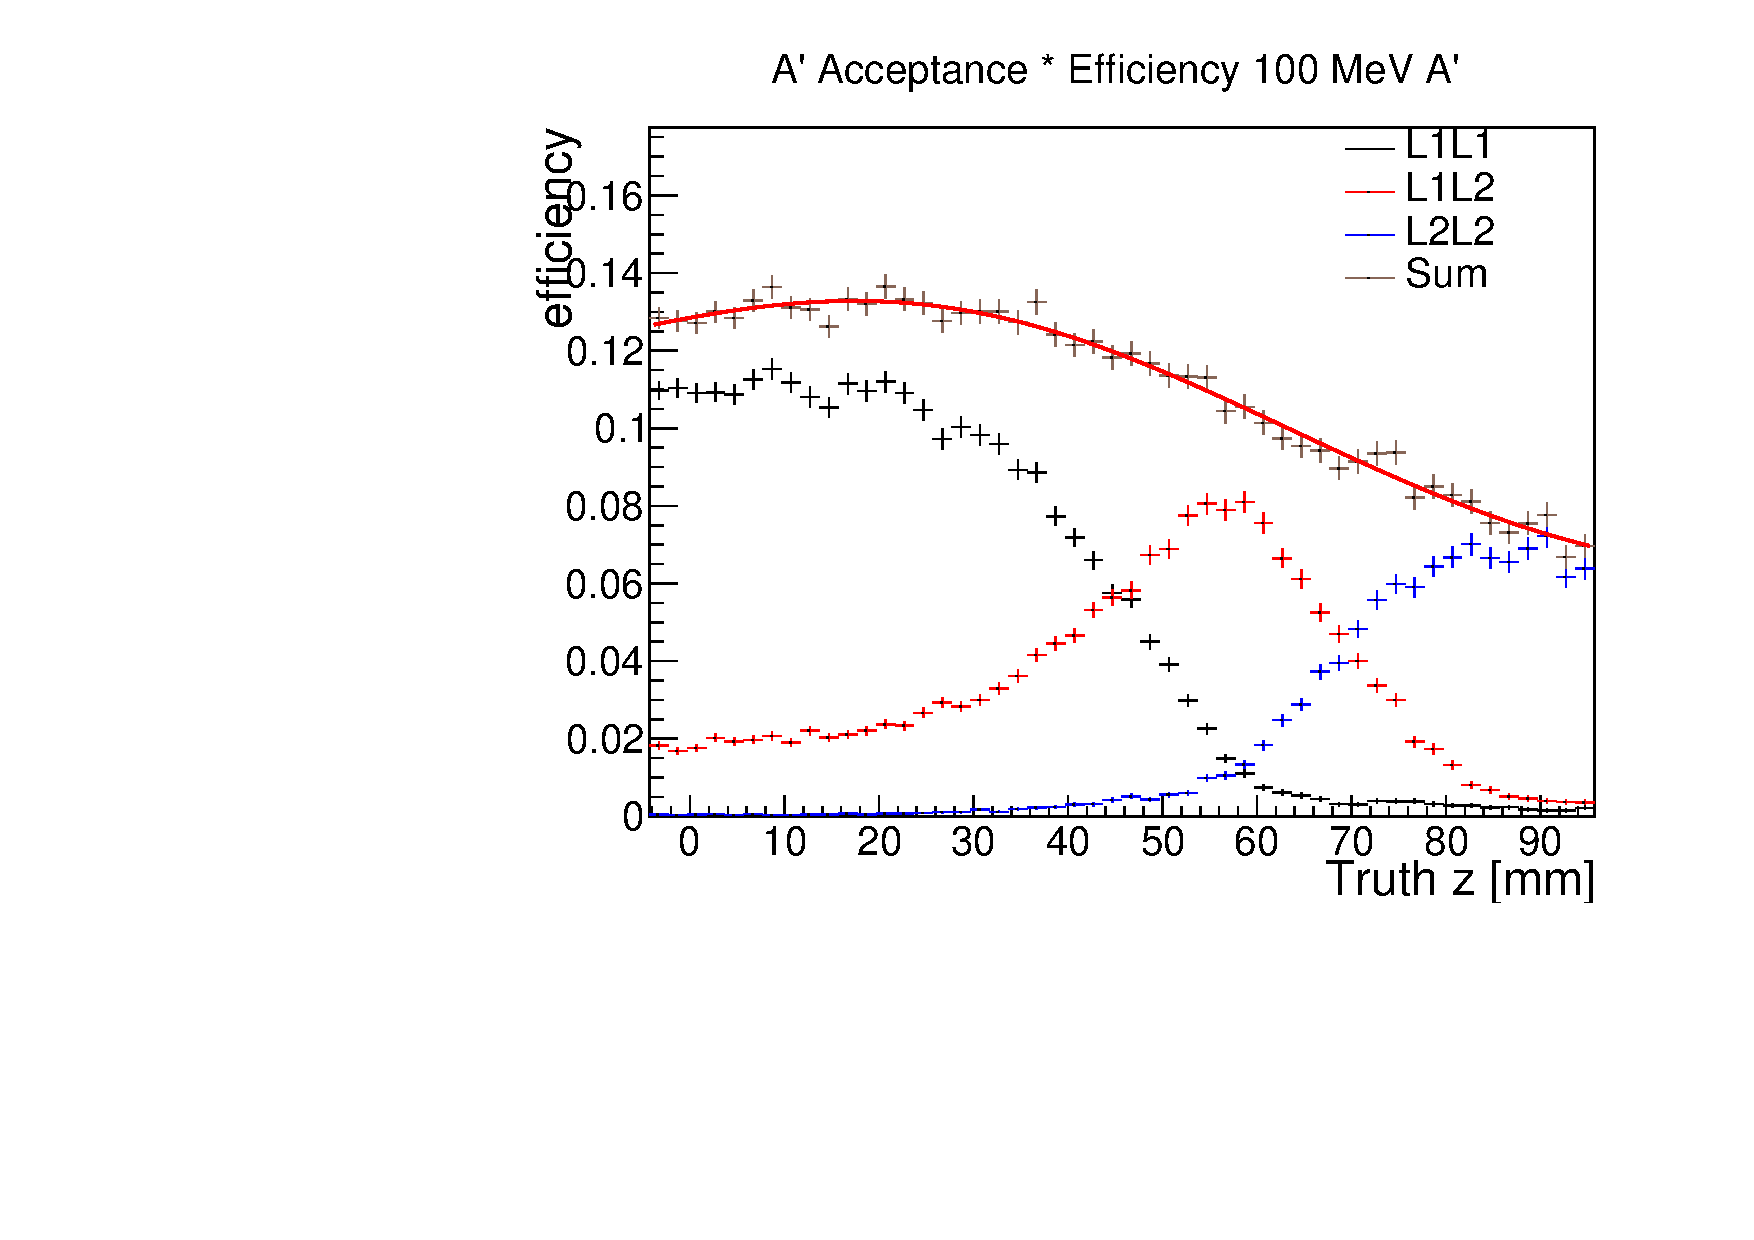
\includegraphics[width=.45\textwidth]{figs/selection/ap_100MeV_eff_fit.pdf}
    \caption{The product of geometrical acceptance and efficiency after the hit killing algorithm for displaced $\aprime$s for the L1L1, L1L2, and L2L2 categories as well as their sum for Left: 80 MeV displaced $\aprime$s and Right: 100 MeV displaced $\aprime$s. %The top is before hit killing and the bottom is with hit killing and a fit function fit to the sum of the categories. \textcolor{red}{The top plots I still have to make, I have the same plots there as the bottom as a placeholder.}
    }
    \label{fig:eff1}
\end{figure}

At this point, the efficiency curves denoted as $\epsilon_{vtx,sum}(z,m_{\aprime})$ are normalized to unity at the target. More specifically, the sum of the mutually exclusive categories is fit and extrapolated to the target position and re-scaled such that $\epsilon_{vtx,sum}(z_{targ},m_{\aprime})=1$. The fit is shown in Fig. \ref{fig:eff1}. However, there are additional tight selection cuts to be applied described in Sec. \ref{sec:apvertexcuts}, and these are applied to the efficiency curves after normalization and shown in Fig. \ref{fig:eff2}.\footnote{There is about a 20\% reduction in signal efficiency from the tight cuts which is why these curves are normalized to $\sim$0.8 at the target.}. To complete the efficiency curves, the signal region must be defined and a description is given in Sec. \ref{sec:tailfits}. As a summary of this procedure, a value of $z$ (denoted as $z_{cut}$) is chosen downstream of which a near-0 background is expected. Thus $z>z_{cut}$ defines the signal region, and this requirement is applied to the reconstructed $z$ of efficiency curves shown in Fig. \ref{fig:eff2}. Finally, to compute the actual expected $\aprime$ yield as a function of $m_{\aprime}$ and $\epsilon$, a re-weighting method is applied where the truth signal distribution is multiplied by these efficiency curves. This process is described in detail in Sec. \ref{sec:signalyeild}.

\begin{figure}[t]
    \centering
    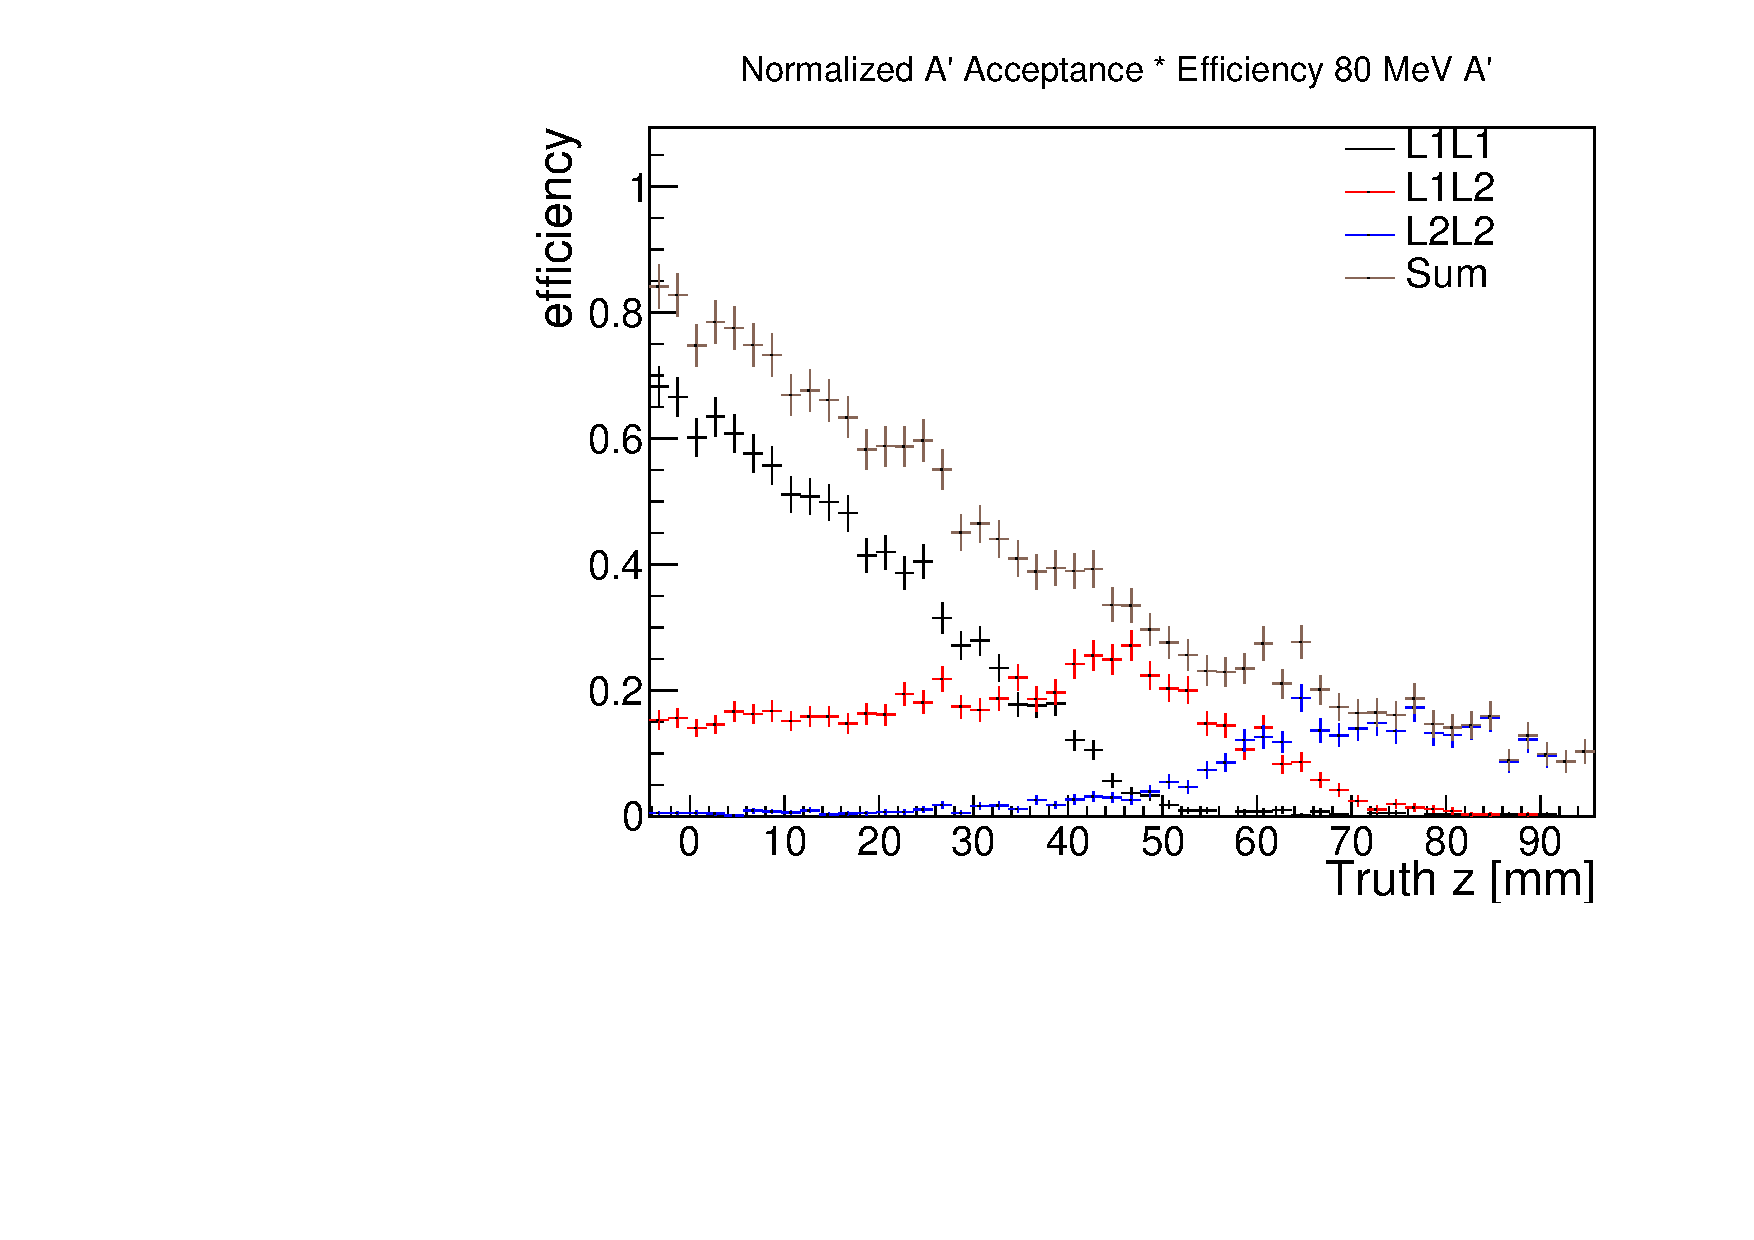
\includegraphics[width=.45\textwidth]{figs/selection/ap_80MeV_eff_norm.pdf}
    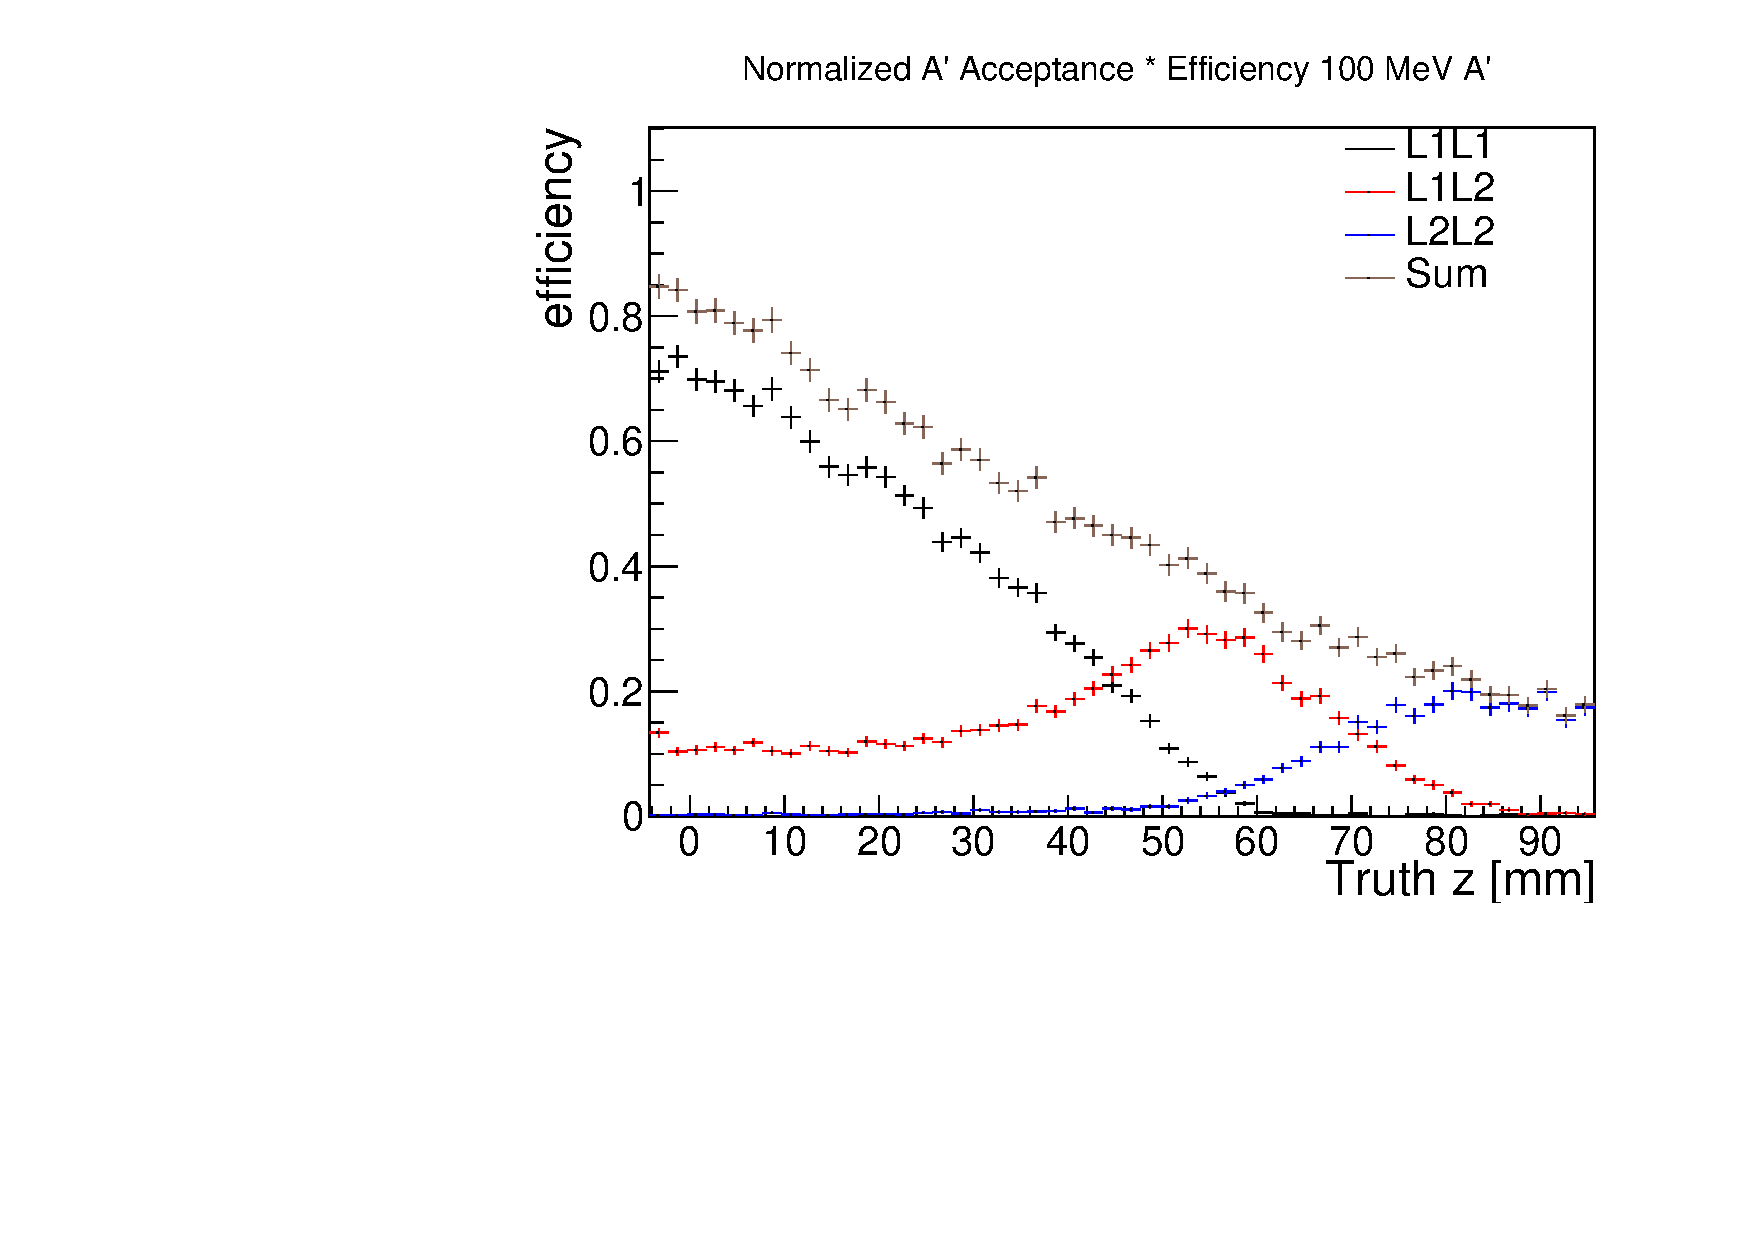
\includegraphics[width=.45\textwidth]{figs/selection/ap_100MeV_eff_norm.pdf}
    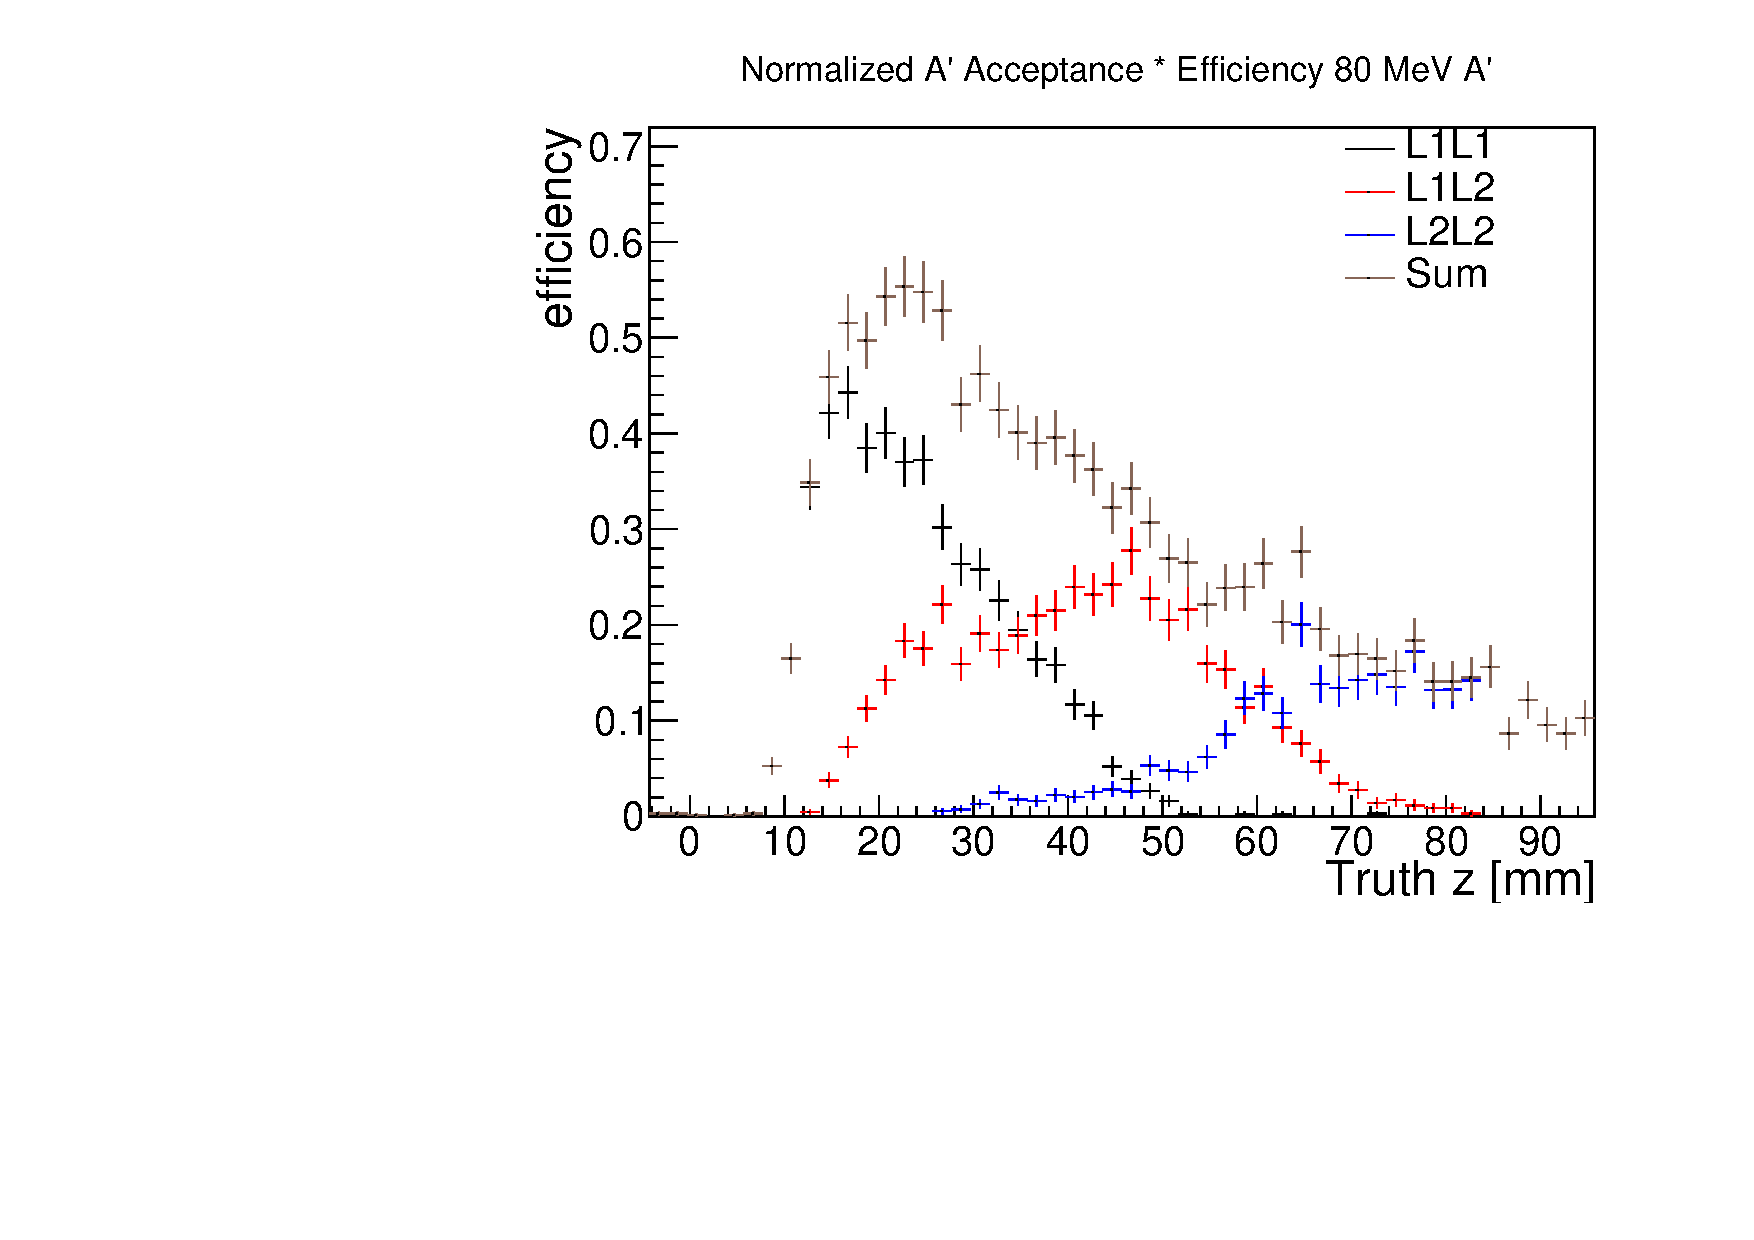
\includegraphics[width=.45\textwidth]{figs/selection/ap_80MeV_eff_norm_zcut.pdf}
    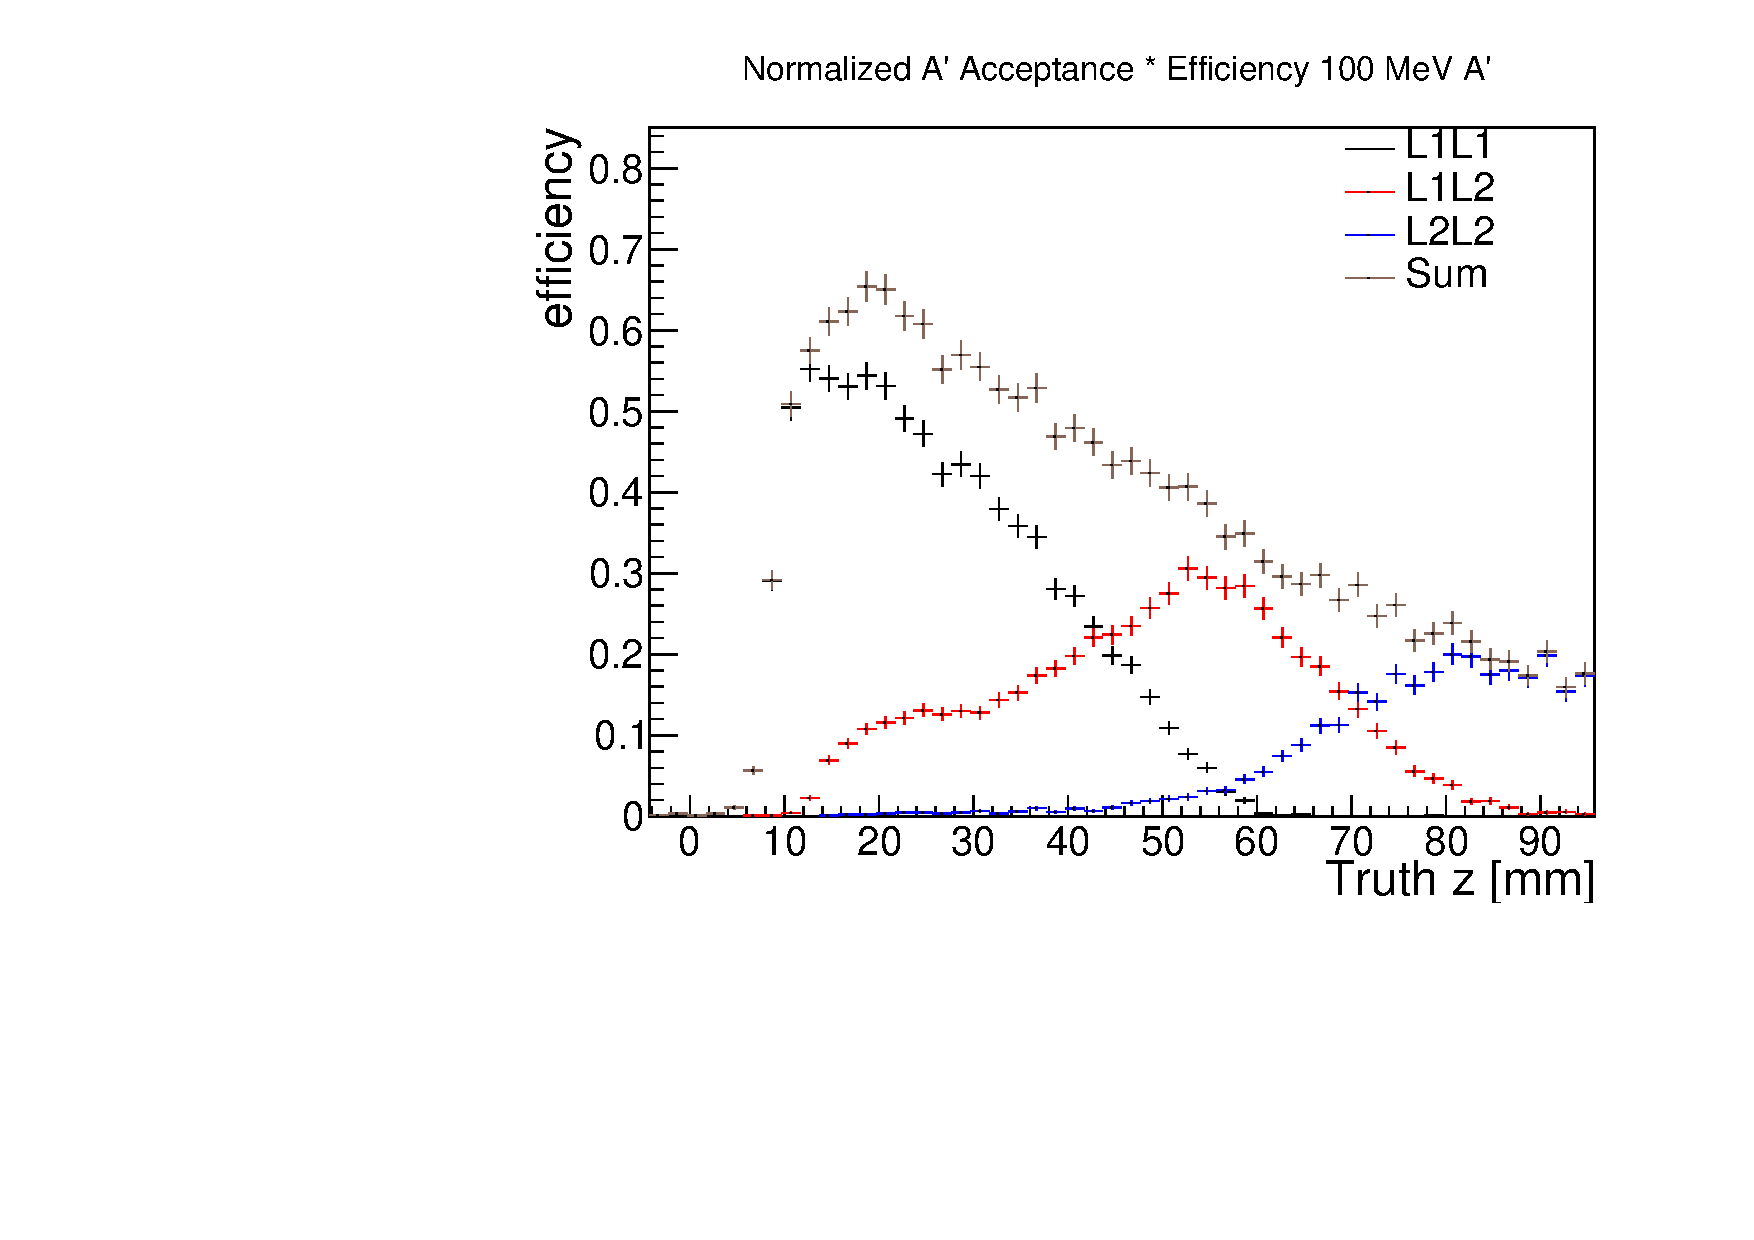
\includegraphics[width=.45\textwidth]{figs/selection/ap_100MeV_eff_norm_zcut.pdf}
    \caption{The product of geometrical acceptance and efficiency for displaced $\aprime$s for the L1L1, L1L2, and L2L2 categories as well as their sum. These plot are normalized to unity at the target, where the sum is normalized before hit killing and further analysis cuts. 80 MeV displaced $\aprime$s are on the left and 100 MeV displaced $\aprime$s are on the right. The top is without the $z_{cut}$ and the bottom is with the $z_{cut}$ from 10\% of the data.}
    \label{fig:eff2}
\end{figure}

\clearpage

\section{Vertex Cuts}\label{sec:apvertexcuts}

The goal of the displaced vertexing analysis is to find long-lived $\aprime$s beyond a background of prompt QED tridents, converted WABs, and beam particles. In order to achieve this, tighter cuts must be utilized such that the prompt background that reconstructs at large $z$, the so-called ``high $z$ background'', is reduced to manageable level such that $\aprime$s can potentially be discovered. Thus, beyond the preselected event cuts, several more cuts are applied to reduce high $z$ backgrounds that otherwise appear signal-like. %in order to further reduce backgrounds at high $z$ that appear otherwise signal-like must be utilized.

A majority of the large $z$ backgrounds result from scattering in layer 1 of the tracker (both the active and dead detector material) or from  mis-reconstructed tracks. Because of this, there are a variety of handles that can be utilized to efficiently distinguish between a true displaced signal and a prompt background. In general, a true displaced signal will have a downstream reconstructed position with good $\chi^2$, a vertex momentum that points back to the beam spot, and be composed of clean tracks with large vertical impact parameters. This is not necessarily true for background. Thus, cuts on impact parameters, projections of the V0 momentum back to the target, and vertex quality are utilized. In addition, to guard against high $z$ background due to mis-tracking the so-called ``isolation cut'' is implemented as well as a minimum V0 momentum cut to kinematically enhance $\aprime$s above Bethe-Heitler tridents.

It is fairly easy to demonstrate the qualitative effectiveness of reducing background without sacrificing too much signal efficiency. Unfortunately, we have no full understanding of background shapes or normalization so it is difficult to be fully quantitative. In order to tune actual cut values beyond the initial qualitative justification, we must rely on only 10\% of the data, a luminosity-equivalent MC sample of tridents overlaid with simulated beam background and WABs, and a three times luminosity-equivalent sample of pure tridents. Although these samples are all informative, this limitation makes it difficult to optimize the cut values in a rigorous quantitative manner. The effectiveness of each tight cut is justified qualitatively by comparing the final vertex $z$ distribution with all the tight cuts and with all the tight cuts except for the cut of interest (i.e. an $n-1$ plot). The 1-D reconstructed $z$ $n-1$ plots for each tight cut is shown in each individual tight cut subsection and the 2-D $n-1$ $z$ vs mass plots are shown in Sec \ref{sec:highz}. In order to be sufficiently justified, each cut must both independently eliminate a significant number of high $z$ events while having minimal impact on signal efficiency. For signal MC, 80 MeV displaced $\aprime$s are chosen for comparisons since this mass is around the peak sensitivity for this dataset. %For those cuts that can't be demonstrated quantitatively, the number of events past $z_{cut}$ (as defined in 10\% of the data) in each sample as well as signal efficiencies are compared for a reasonable decision, where the number of events past $z_{cut}$ are scaled to 10\% of the data (divided by 10 for tritrig-wab-beam and divided by 30 for tritrig).

$\aprime$s with a relatively short decay length will have layer 1 hits for both daughter particles, while $\aprime$s with longer decay lengths may have one or both of these particles miss layer 1 due to geometrical acceptance as shown in Fig. \ref{fig:L1L2_L1L2_schem}. For prompt background, even though the SVT is designed to maintain the same acceptance in all layers at 15 mrad, several ``real world'' effects cause particles to sometimes miss a layer in the detector. First, hit efficiencies in layer 1 may cause particles to miss layer one even though the particle traverses the active sensor plane. In addition, daughter particles (or photon conversions) can interact with the dead material in layer 1 and force the particle to scatter into the acceptance of the detector. These effects are shown in Fig. \ref{fig:L1L2_background}.


%\begin{figure}[t]
%    \centering
%    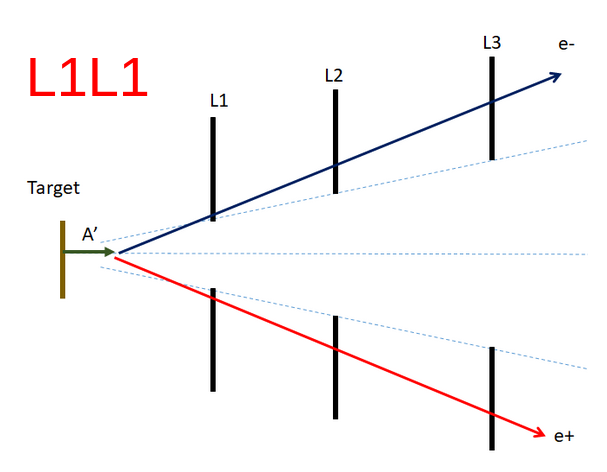
\includegraphics[width=.45\textwidth]{figs/selection/L1L1_schem.png}
%    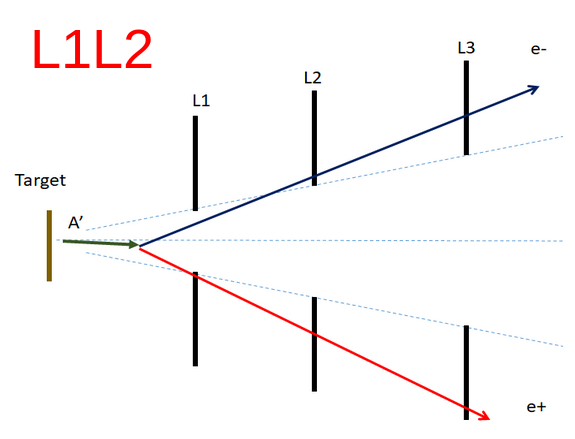
\includegraphics[width=.45\textwidth]{figs/selection/L1L2_schem.png}
%    \caption{Left: Schematic of a relatively short $A'$ decay length in which both daughter particles have a layer 1 hit. Right: Schematic of a relatively long $A'$ decay length in which one of the daughter particles misses layer 1 (but hits layer 2) and the other daughter particle hits layer 1.}
%    \label{fig:L1L2_L1L2_schem}
%\end{figure}

\begin{figure}[t]
    \centering
    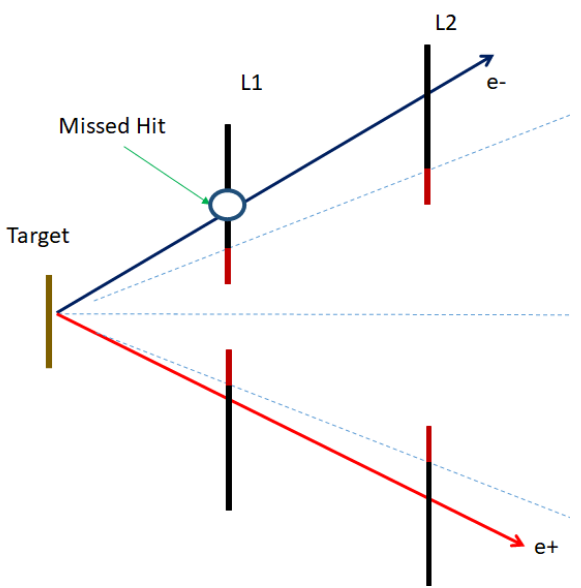
\includegraphics[width=.45\textwidth]{figs/selection/L1L2_background1.png}
    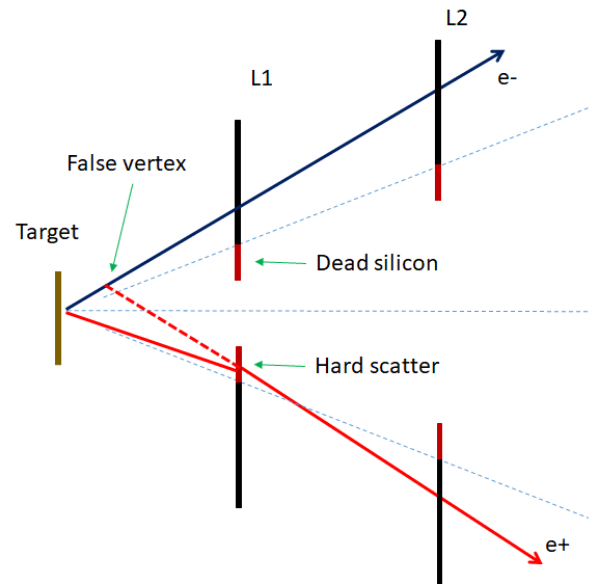
\includegraphics[width=.45\textwidth]{figs/selection/L1L2_background2.png}
    \caption{Left: A schematic of a prompt background process that has a hit inefficiency in layer 1 and is placed in the L1L2 category. Right: A schematic of a prompt background process in which one of the daughter particles scatters away from the beam in the inactive silicon of layer 1 and into the acceptance of the tracker. This process is placed in the L1L2 category and also reconstructs a false vertex downstream of the target.}
    \label{fig:L1L2_background}
\end{figure}

Thus, the analysis is divided into several mutually exclusive categories based on the first hits on track of the two daughter particles similar to how signal is divided in Sec. \ref{sec:aprimerate}. If both particles have a layer 1 hit, the event is placed in the so-called L1L1 category. If exactly one particle hits layer 1 and the other particle misses layer 1, the event is placed in the L1L2 category. If both particles miss layer 1, event is placed in the L2L2 category. These are the only three categories since tracking algorithms require 5 hit tracks in a 6 layer detector. For the purposes of this analysis, only the L1L1 and L1L2 categories are used since the probability of further downstream decays decreases exponentially such that the L2L2 category adds minimal significance to the analysis. 

Performing the analysis on these categories separately instead of together is done for several reasons. First, the vertex resolution is highly dependent on which layers are hit first. The closer the first hit to the target the better the vertex resolution (i.e. L1L1 has better vertex resolution than L1L2 which has better resolution than L2L2). Second, the nature of the backgrounds between the categories are different. The L1L1 category high $z$ backgrounds are typically due to multiple scattering in the active region of L1 sensors and mis-tracking while backgrounds in the L1L2 and L2L2 categories are typically due to hit efficiency effects, multiple scattering in both active and inactive regions of layer 1, converted WABs, mis-tracking, and even trident production in layer 1. 

\clearpage

\subsection{L1L1}\label{sec:apL1L1}

%\flushleft{\textbf{L1L1 Layer Requirements}}
\textbf{L1L1 Layer Requirements}

For the L1L1 category, layer 1 hits on both $\epem$ tracks are required. In addition to requiring layer 1 hits, layer 2 hits are also required which improves the resolution for extrapolating tracks to the correct hit in layer 1. This has the effect of reducing mis-tracking which can result in high $z$ backgrounds (see isolation cut subsection). Layer 3 hits are not explicitly required by the analysis, rather they are implicitly required by the SeedTracker algorithm. Thus, all events in this category have hits in layers 1-3. %The effect of requiring layer 1 and layer 2 hits is shown in Fig. \ref{fig:L1L1_L1L1}.
A summary of the tight selection cuts in the L1L1 category is shown in Table \ref{tab:L1L1cuts} and described in the following subsections.


\begin{table}[!hb] 
    \centering
    \begin{tabular}{lr}
        \toprule
        \textbf{Cut Description} & \textbf{Requirement} \\
        \midrule
        Layer 1 Requirement & $e^+$ and $e^-$ have L1 hit \\
        Layer 2 Requirement & $e^+$ and $e^-$ have L2 hit \\
        %Tight Vertex Quality & $\chi^2_{unc} < 4$ \\
        Radiative Cut & $V_{0p} > 1.85$ GeV \\
        V0 projection to target & Fitted 2$\sigma$ cut \\
        Isolation Cut & Eq. \ref{equ:iso_final_simple} \\ %$\delta+\frac{1}{2}(z0+z_{targ} \ \frac{P_Y}{P} \ $sign$(P_Y)) > 0$ \\
        Impact Parameters & Eq. \ref{equ:z0_cut_final} \\
        %Vertex Errors & TBD \\
        \bottomrule
    \end{tabular}
    \caption{A summary of the tight cuts for the L1L1 category.}
    \label{tab:L1L1cuts}
\end{table}

\clearpage

\textbf{Projection of the vertex to the target}


As mentioned previously, in order to reduce the number of downstream high $z$ background events, it is required that vertices project back to the beamspot position. The vertex projection to the target in the $x-y$ plane is computed by taking the direction of the vertex momentum, computed as the vector sum of the momenta of the $\epem$ pair, and extrapolating the vertex position to the target location (at $z=$-4.3 mm in detector coordinates). While in MC simulation the beamspot is generated in a fixed position, the position of the unconstrained vertices in the $x-y$ plane in data depends on the beam conditions, leading to run-by-run biases that need to be corrected before applying the target projection cut. 

\begin{figure}[t]
    \centering
    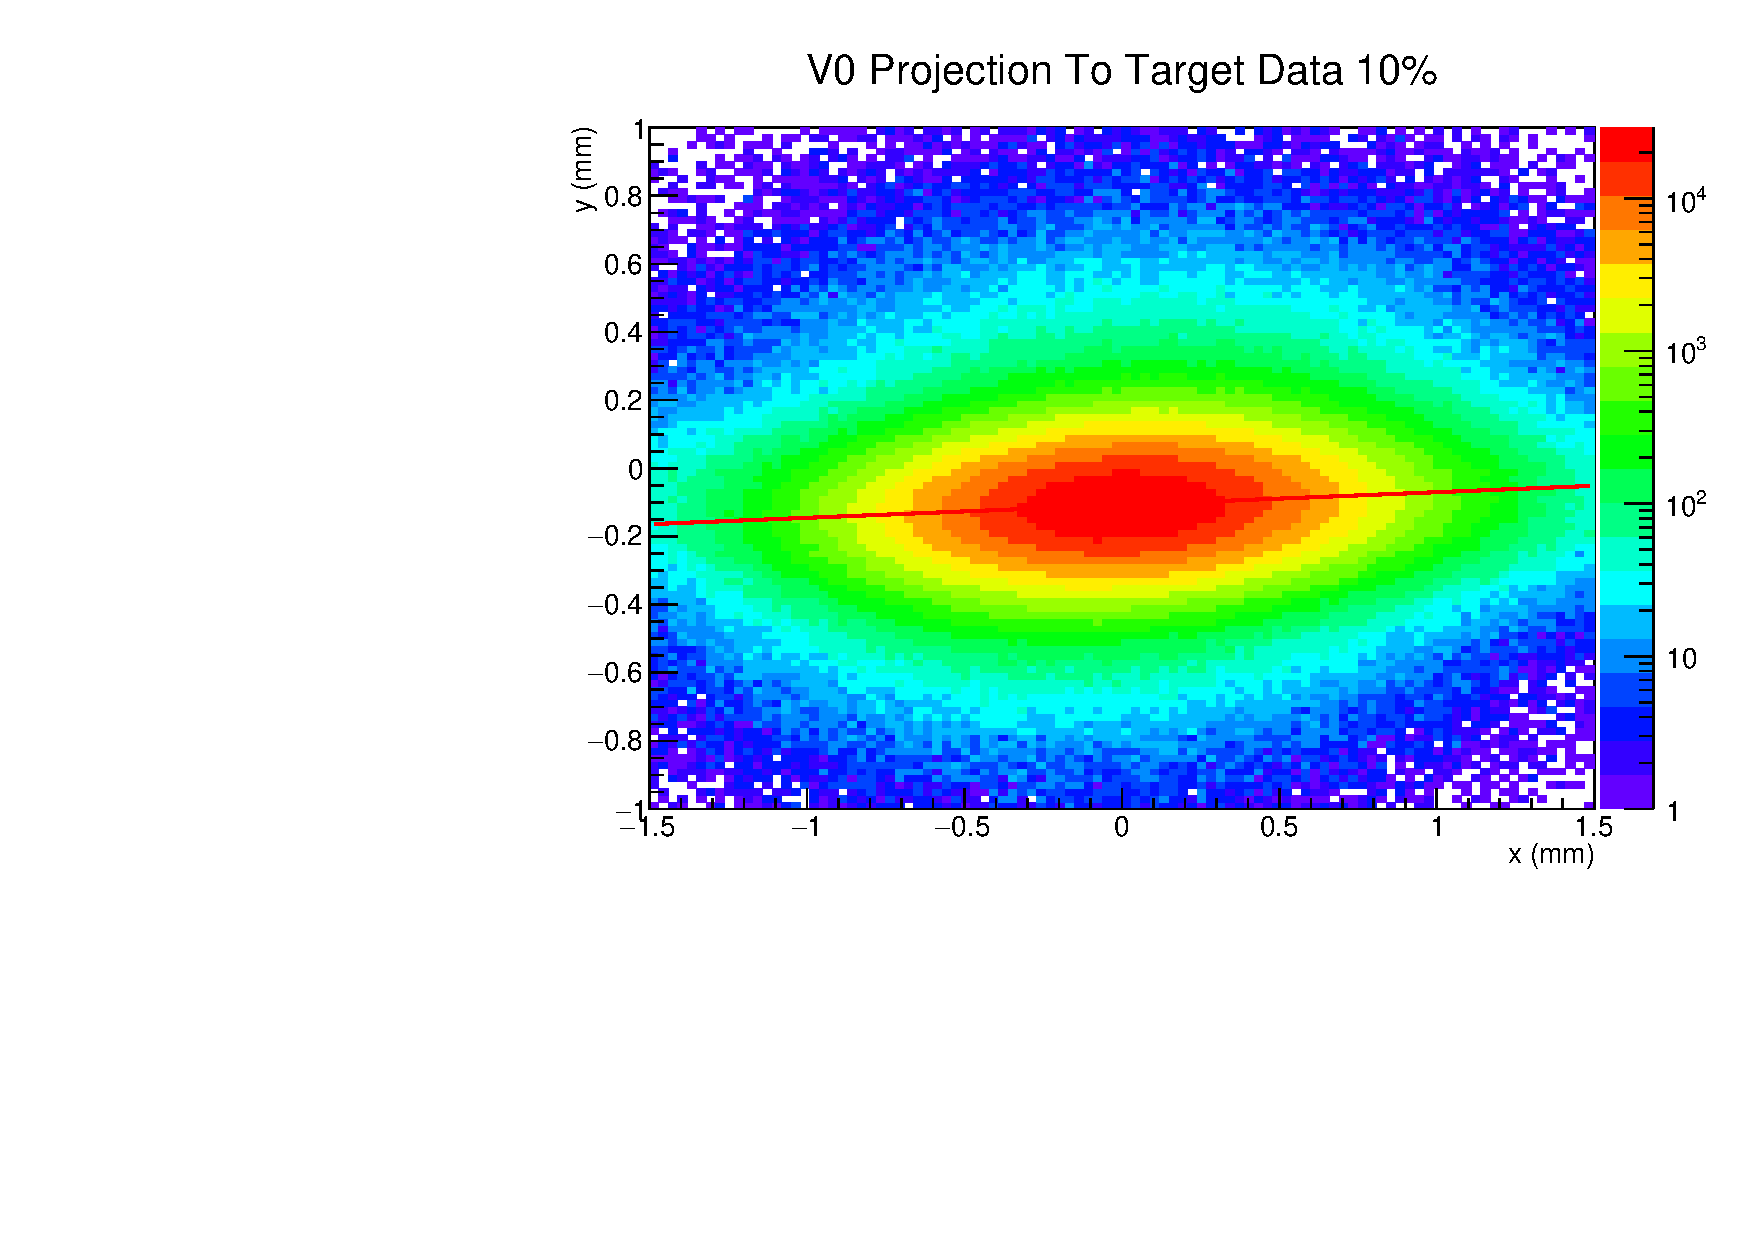
\includegraphics[width=.45\textwidth]{figs/selection/10per_data_L1L1_V0proj.pdf}
    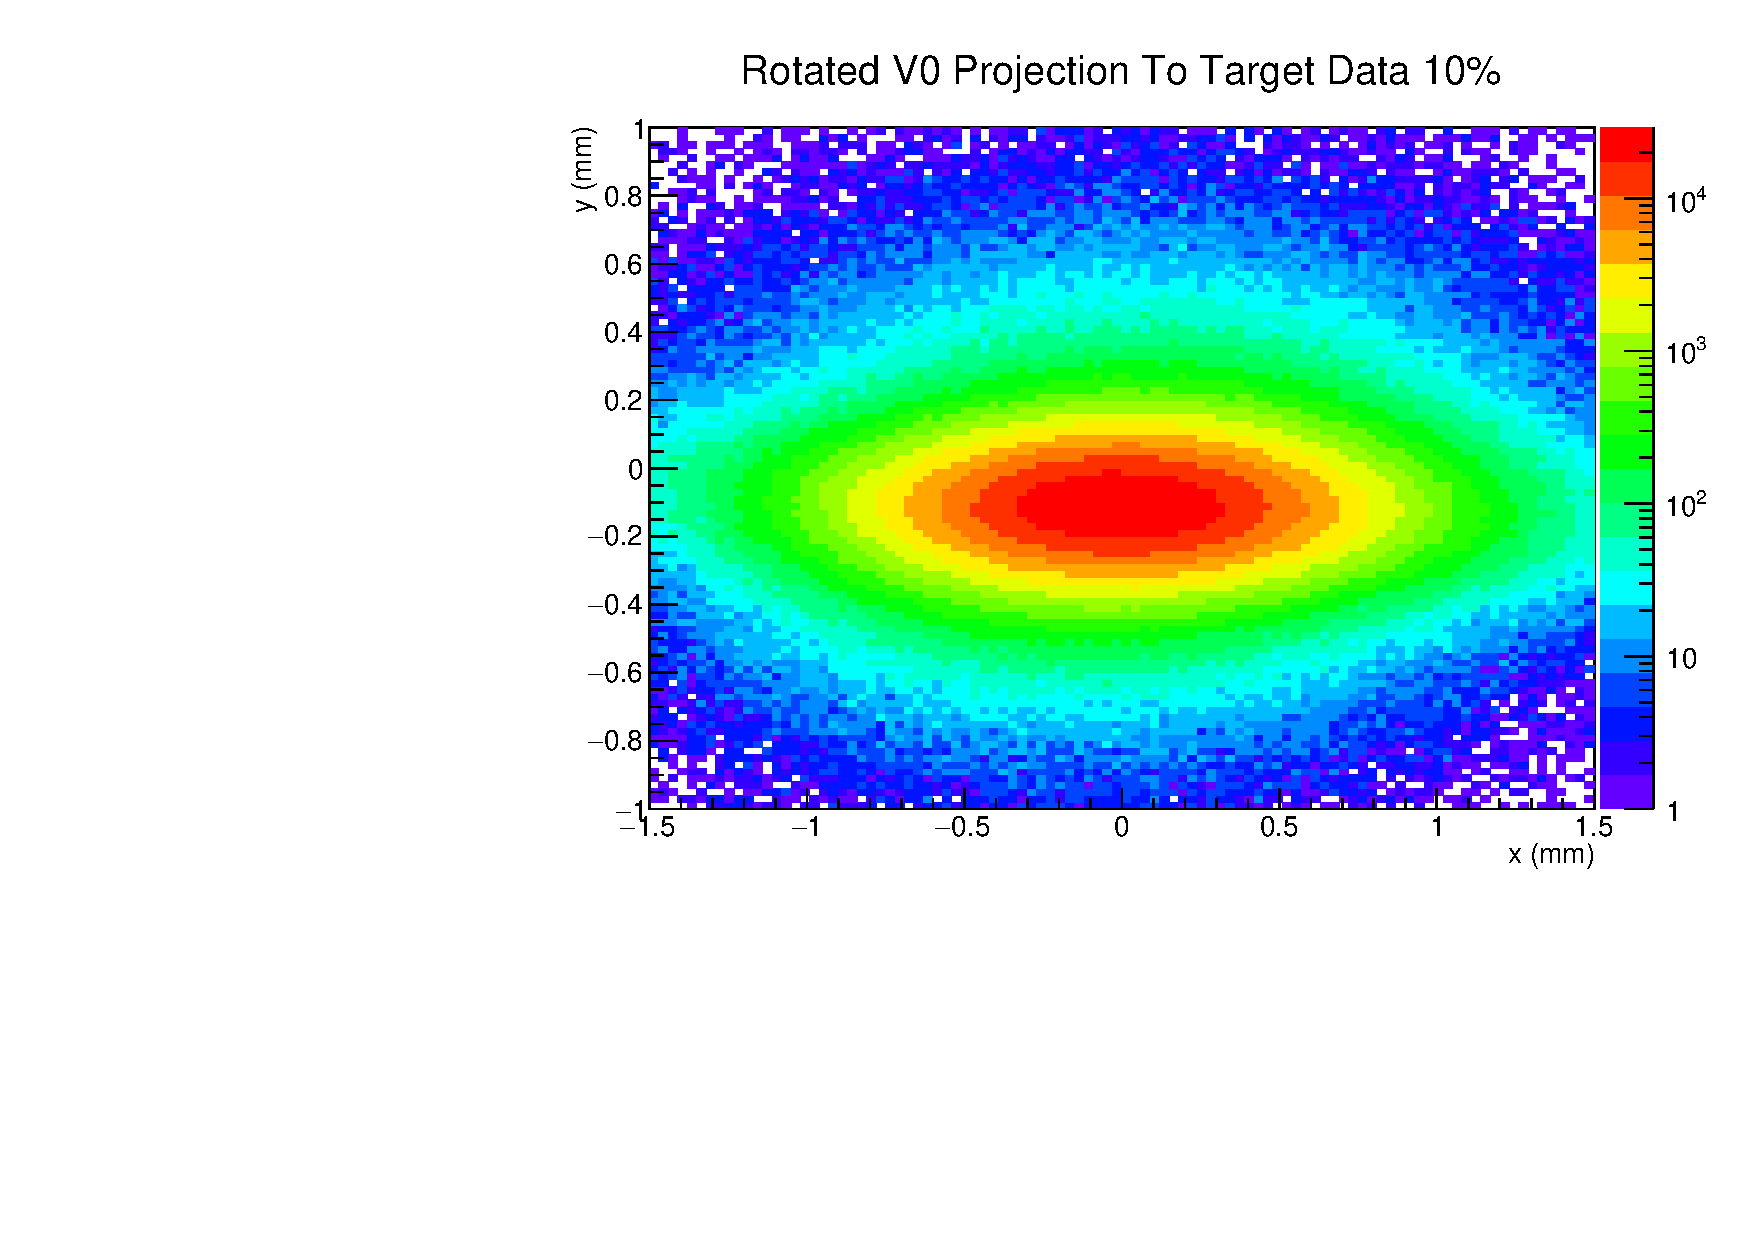
\includegraphics[width=.45\textwidth]{figs/selection/10per_data_L1L1_V0proj_rot.pdf}
    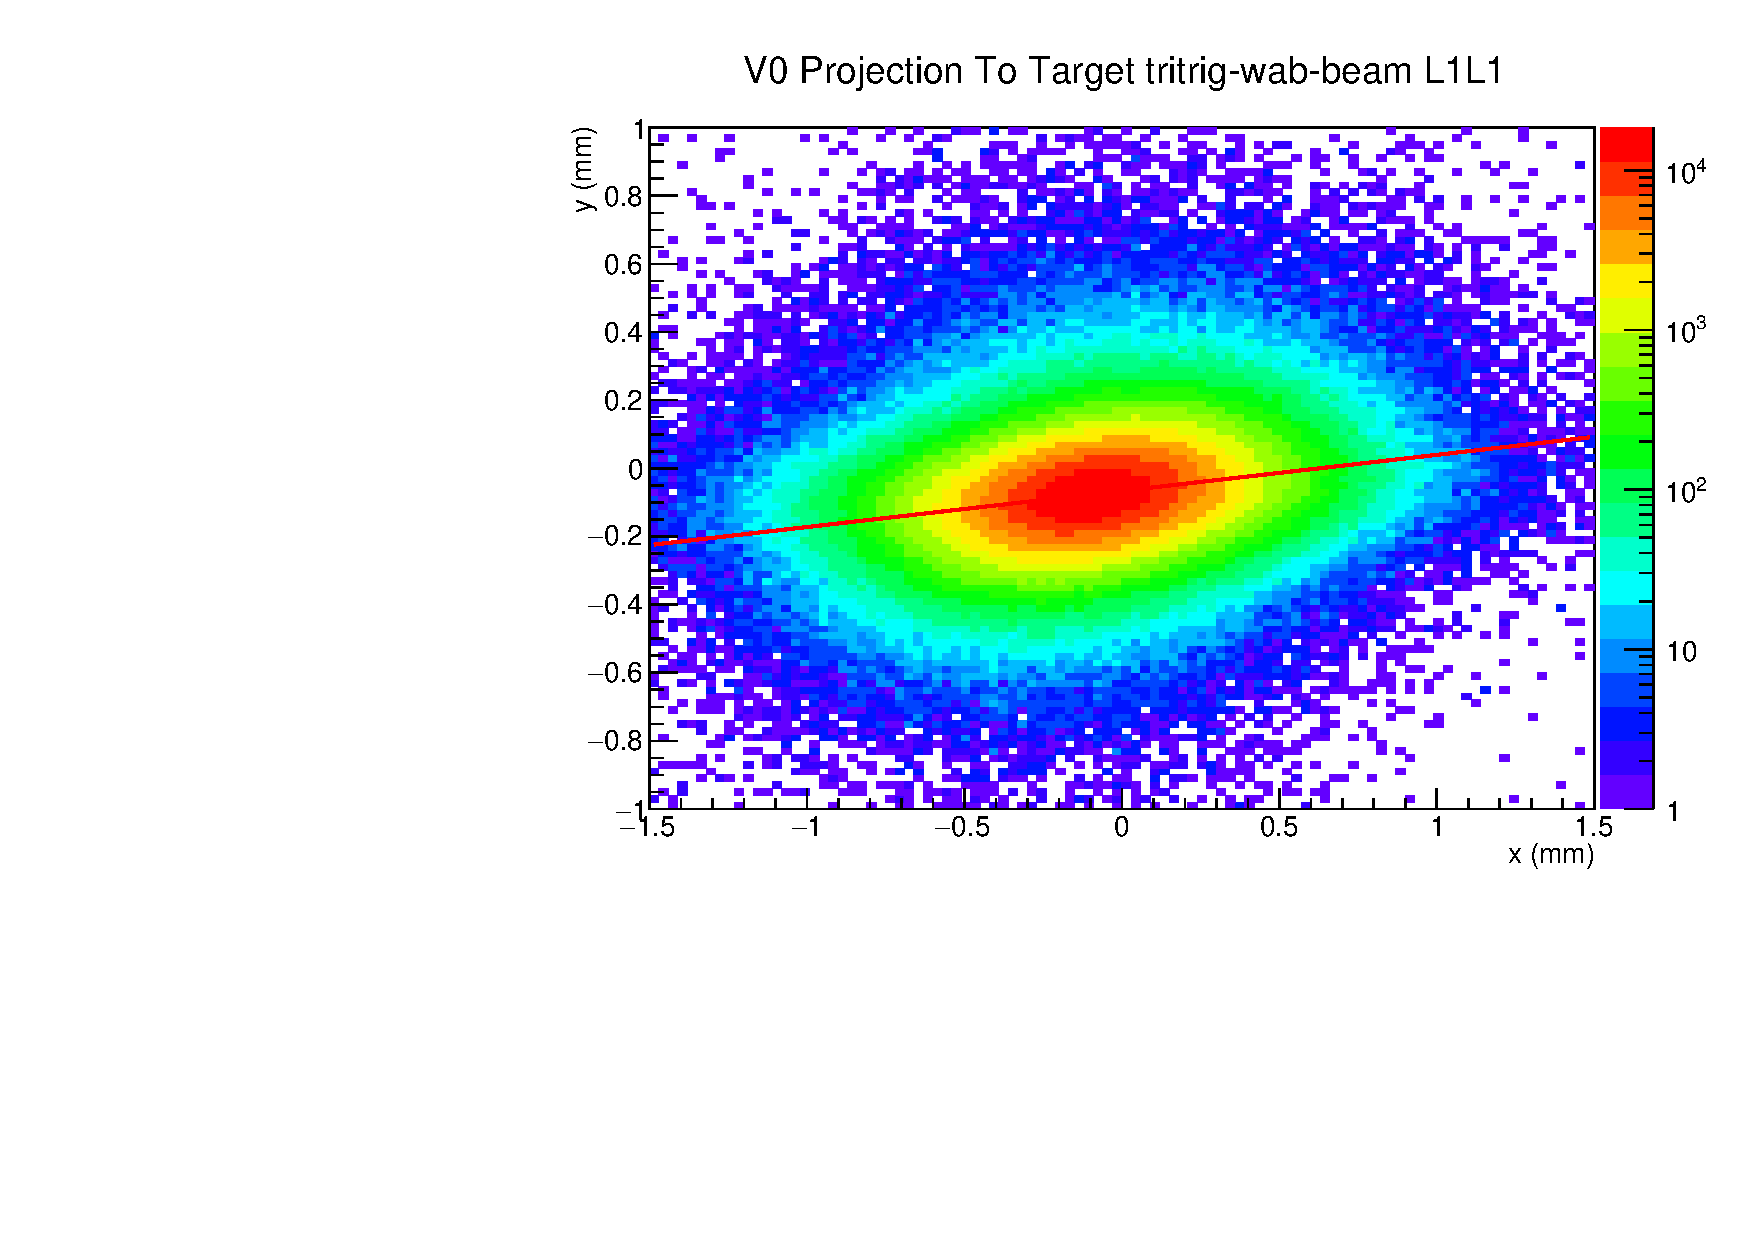
\includegraphics[width=.45\textwidth]{figs/selection/tritrig-wab-beam_L1L1_V0plots_V0proj.pdf}
    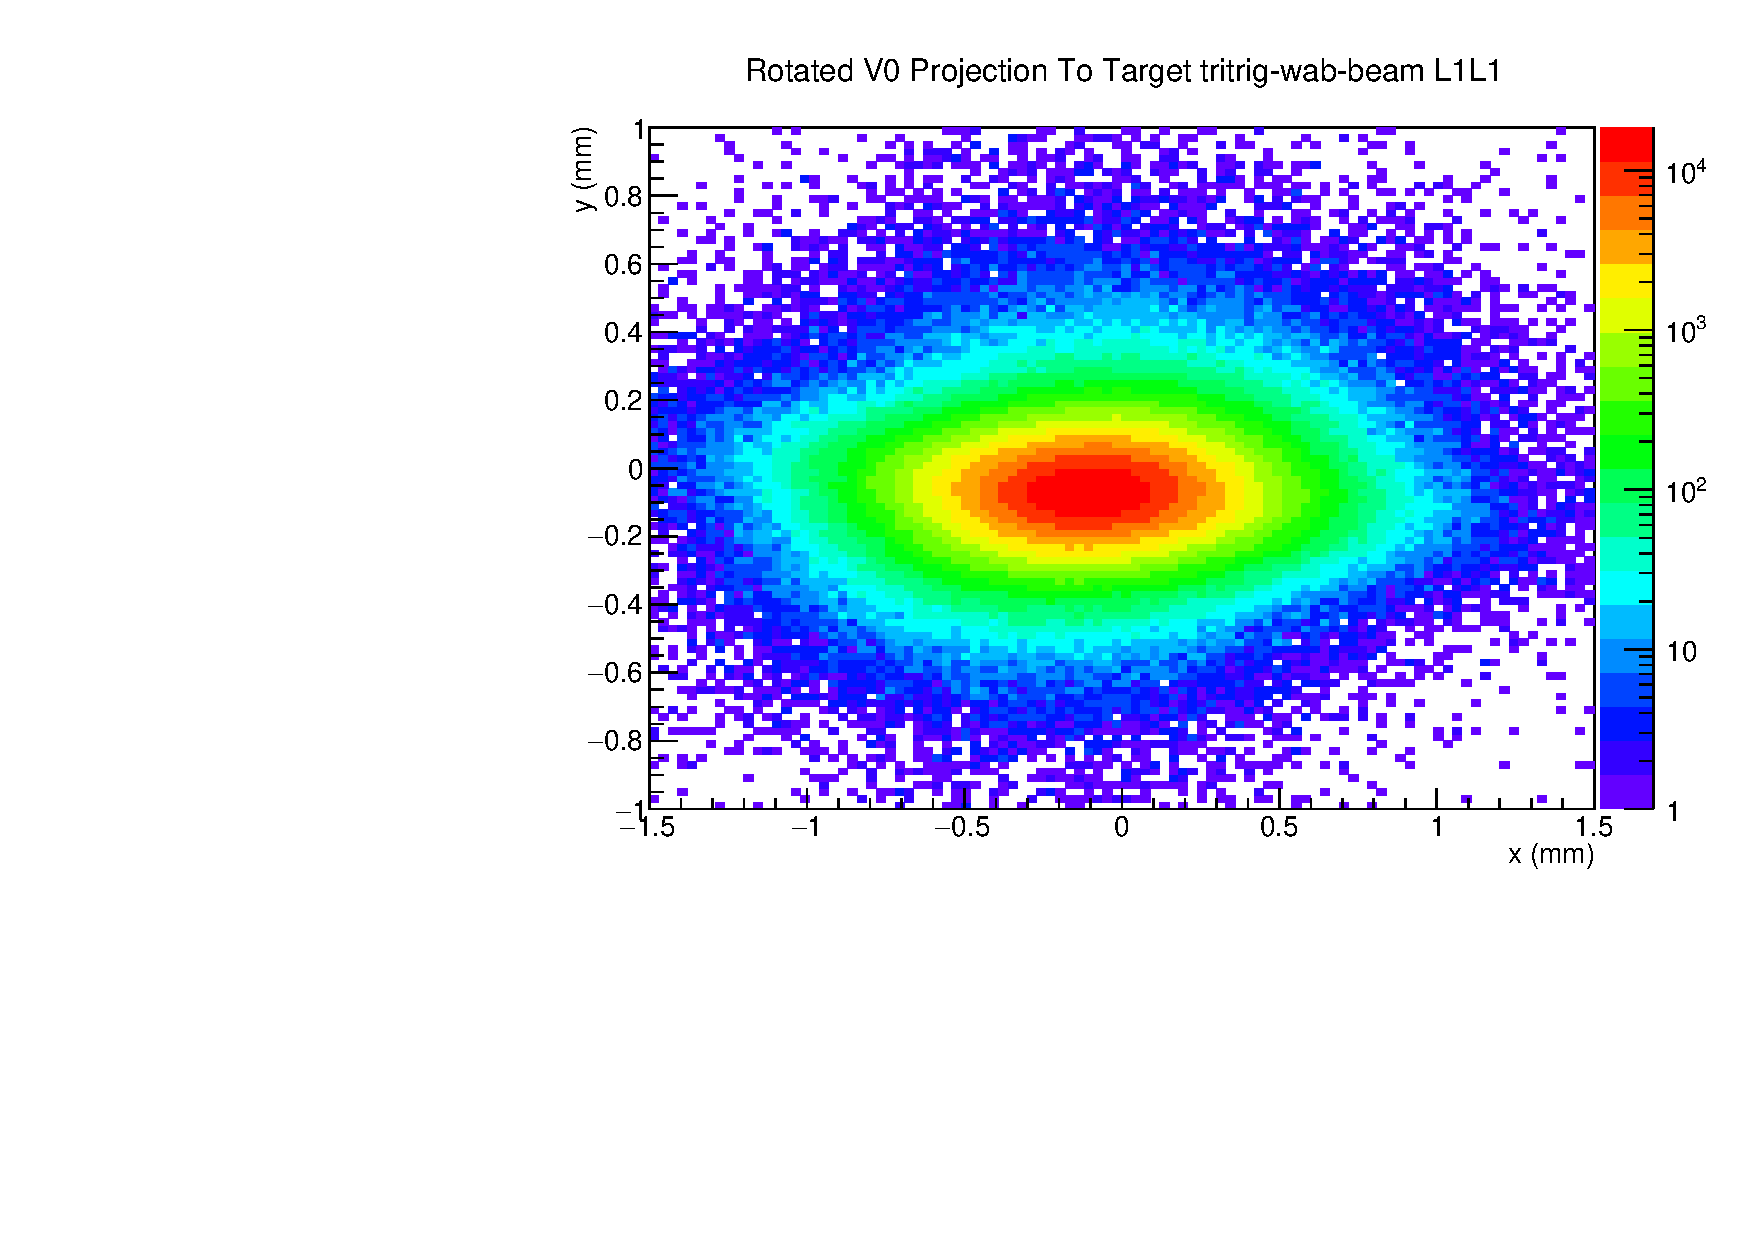
\includegraphics[width=.45\textwidth]{figs/selection/tritrig-wab-beam_L1L1_V0plots_V0proj_rot.pdf}
    \caption{The V0 projection back to the target for Preselection in the L1L1 category. Upper Left: 10\% Data with a linear fit to the $x$-$y$ correlation Lower Left: 10\% tritrig-wab-beam with a linear fit to the $x$-$y$ correlation. The V0 projection back to the target for L1L1 Preselection with rotated $x$-$y$ coordinates for Upper Right: 10\% Data and Lower Right: 10\% tritrig-wab-beam. The angle of rotation is $\theta_{data}=0.0387$ rad in data and $\theta_{MC}=0.1110$ rad in MC. }
    \label{fig:targ_proj}
\end{figure}

The longitudinal and transverse spatial distributions of the vertices that pass the Preselection cuts are used to estimate the run-by-run position of the beamspot in data and MC simulation. The spatial distributions are fit with a Gaussian function in the interval [-1.5RMS, 1.5RMS], where RMS is the root mean square of the distributions. The same procedure is applied to the distributions for the transverse projections of the vertex to the target surface. 

The transverse projections show correlation between the $x$ and $y$ coordinates of the extrapolations in Fig. \ref{fig:targ_proj} in both data and MC, although different correlations. The linear correlation was fit in the interval [-0.5 mm, 0.5 mm] in order to fit the correlation in the core of the distribution. The angle in data, across all 10\%, is $\theta_{data}=0.0387$ rad and in a subset of tritrig-wab-beam $\theta_{MC}=0.1110$ rad. The rotation is also shown Fig. \ref{fig:targ_proj}. The new rotated coordinates are then refit using the method above to determine the rotated $x$ and $y$ fitted means and sigmas in MC and on a run-by-run basis for data. These values are used to form an elliptical cut on the rotated $x$ and $y$ coordinates in units of $n_{\sigma}$ from the mean.

% $\theta_{data}=0.0386557750132$ rad
%tritrig-wab-beam $\theta_{MC}=0.111025680707$ rad

%In Figure \ref{fig:rundepposz} the mean of the longitudinal position for data and MC simulation is shown. In Figure \ref{fig:rundepposxy} and 
In Figure \ref{fig:rundepposxys}, the mean and width of the transverse projection to the target surface, with rotations for the $x$ and $y$ coordinates are shown for data and MC. These are used for the run-by-run corrections in data. The actual cut value, which is reduced to a single tuneable parameter $n_{\sigma}$ from the mean, is difficult to optimize because we currently do not have a viable model of high $z$ backgrounds with sufficient statistics. However as a quick study, the cut value was floated and the ratio of the expected signal yield (at two optimal mass and $\epsilon$ points) to the background (taken across the entire signal range) was computed. It was determined by this metric (the maximum signal to background ratio) that the final result is generally independent in the cut range from $n_{\sigma}=2$ to $n_{\sigma}=3$. From this study, the cut is selected as $n_{\sigma}=2$ and is shown in Fig. \ref{fig:targ_proj_cut}. The effectiveness of this cut (and all the tight cuts) is justified qualitatively by comparing the final reconstructed $z$ distribution with all the tight cuts and with all the tight cuts except for the projection back to the target cut (i.e. an $n-1$ plot). This is shown for both 10\% of the data and an 80 MeV $\aprime$ in which a large number of events on the tail and high $z$ events are eliminated with minimal impact on the signal efficiency. %The 2 of the V0 projection cut is shown in Fig. \ref{fig:v0proj_L1L1} including the final selection with and without the projection cut (i.e. an $n-1$ plot). %The effect of floating the value of the V0 projection cut is shown in Fig. \ref{fig:floatcut_v0proj_L1L1}.

%The actual cut value is difficult to demonstrate quantitatively. Table \ref{tab:V0proj_L1L1_80} and Table \ref{tab:V0proj_L1L1_100} show the effect of the V0 projection cut on high $z$ events (events past $z_{cut}$ from the 10\% data) on 10\% data, 100\% tritrig-wab-beam sample, and x3 tritrig sample as well as 80 MeV and 100 MeV displaced $A'$s. From this data, a circular cut on the rotated projections is set to $2\sigma$ from the mean and is shown in Fig. \ref{fig:targ_proj_cut}. The effect of the V0 projection cut is shown in Fig. \ref{fig:v0proj_L1L1}. The effect of floating the value of the V0 projection cut is shown in Fig. \ref{fig:floatcut_v0proj_L1L1}.

\begin{figure*}[t!]
    \centering
    %\begin{subfigure}[t]{0.45\textwidth}
    %    \centering
        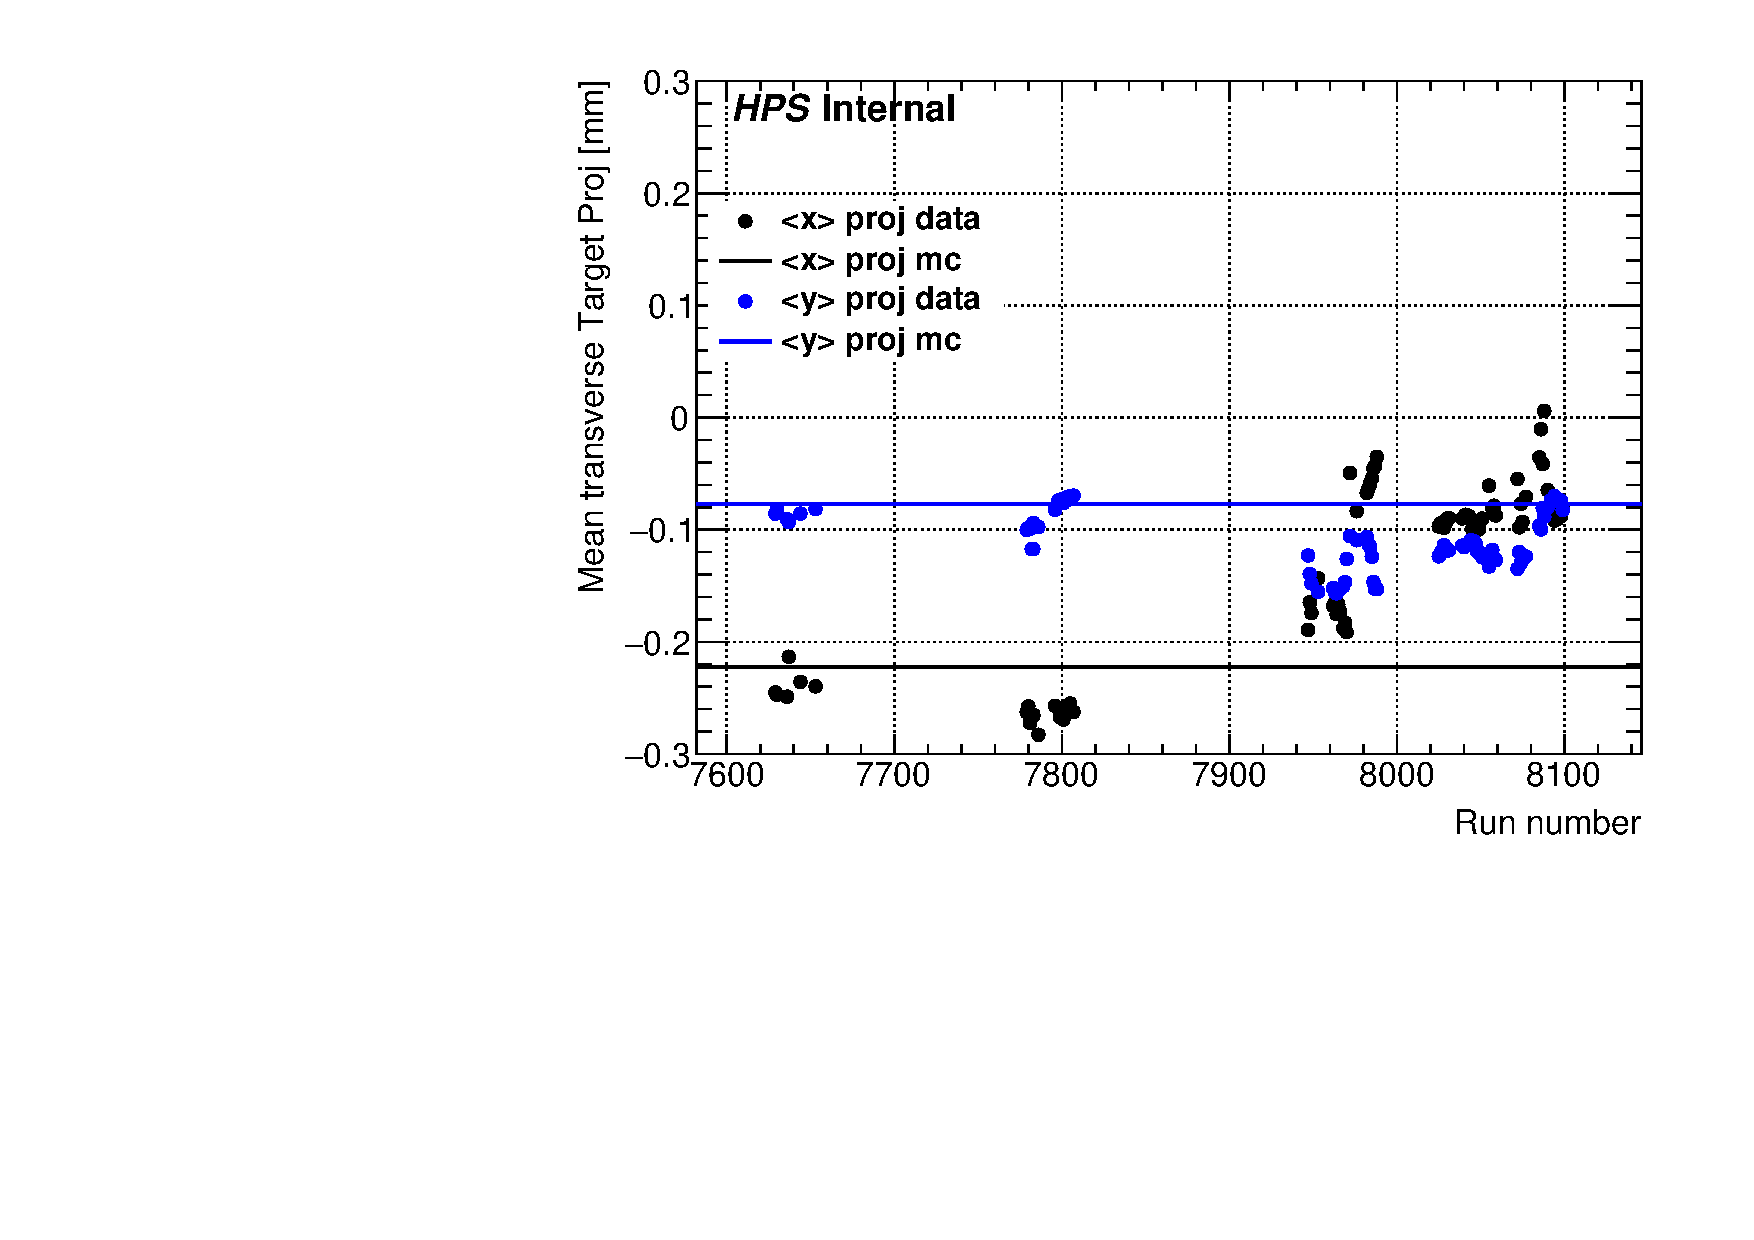
\includegraphics[width=.85\textwidth]{figs/recon/xy_proj_final.pdf}
    %\caption{}
    %\end{subfigure}%
    %~ 
    %\begin{subfigure}[t]{0.45\textwidth}
    %    \centering
        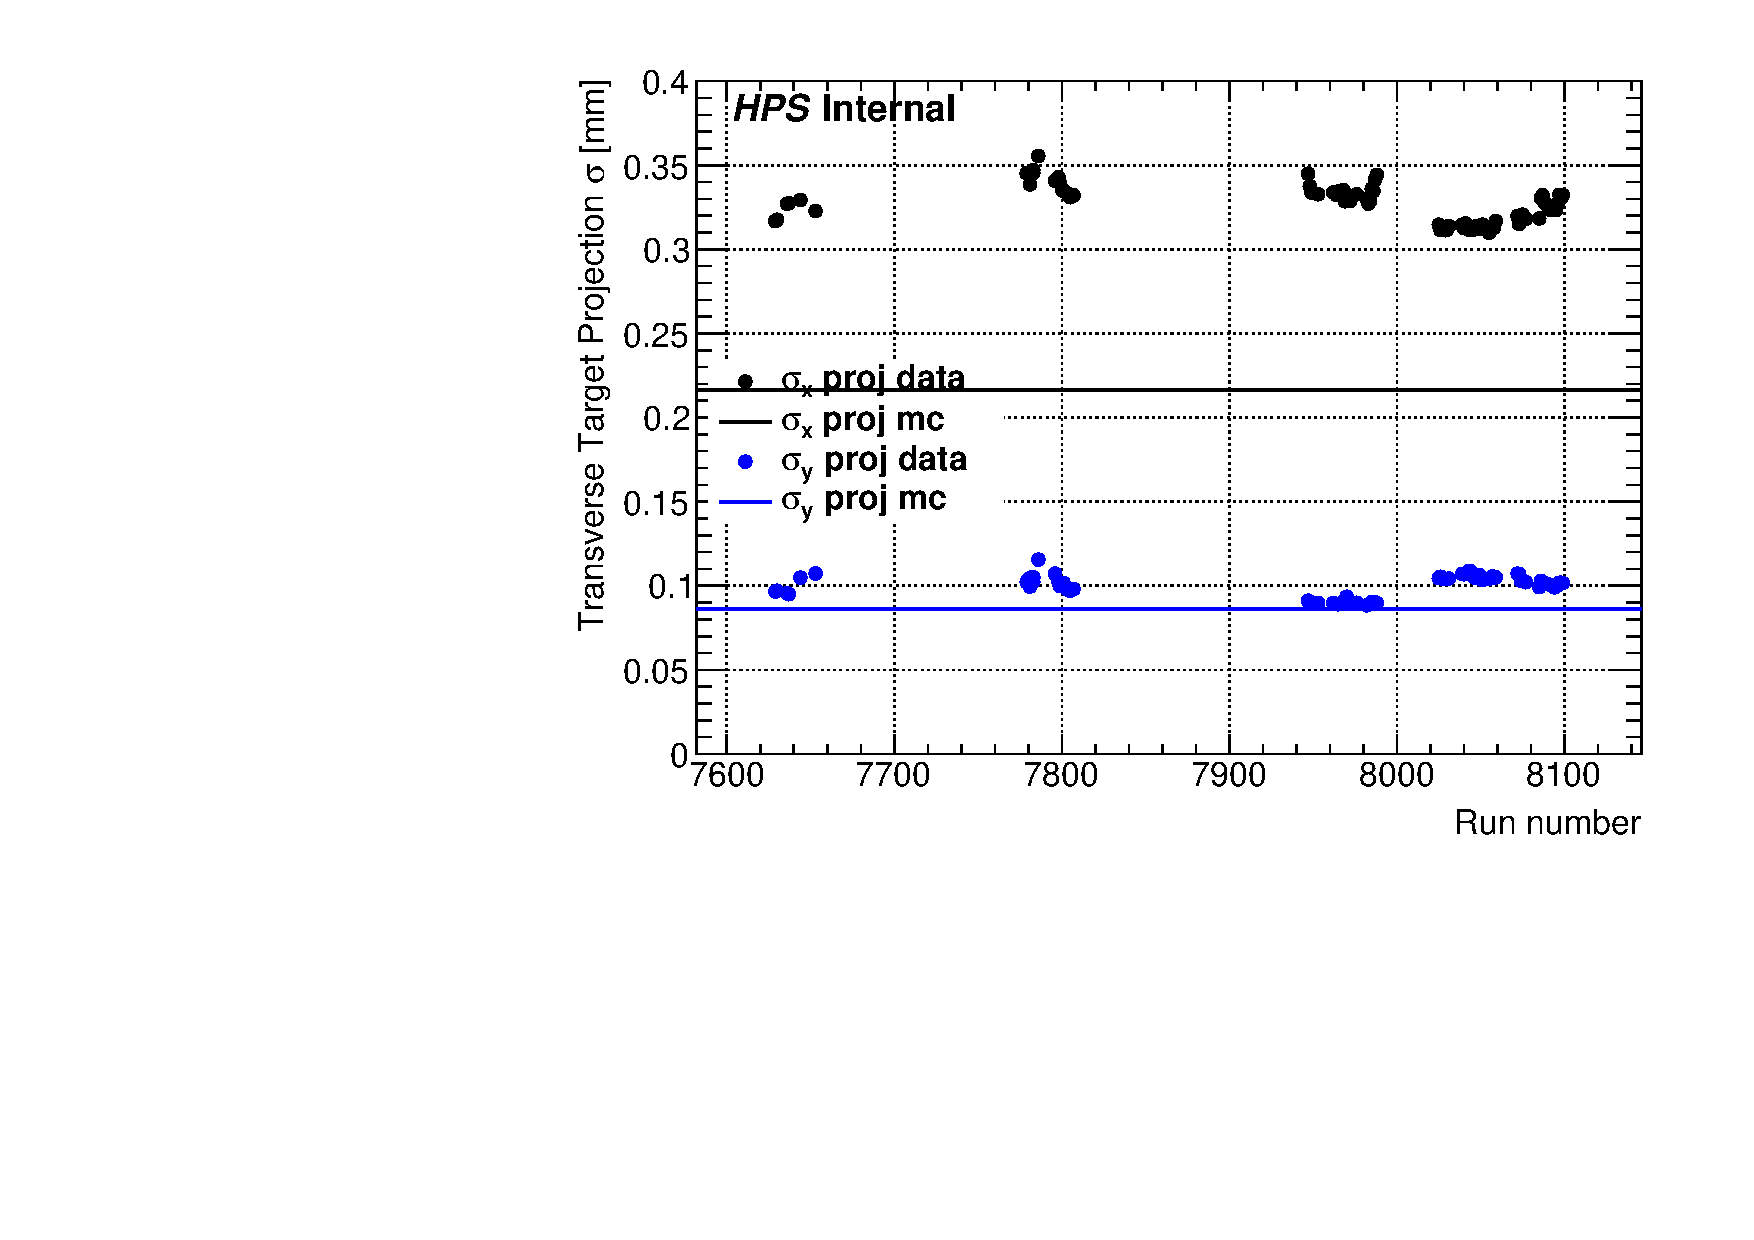
\includegraphics[width=.85\textwidth]{figs/recon/sigma_xy_proj_final.pdf}
    %    \caption{}
    %\end{subfigure}
    \caption{The run-dependent mean (left) and width (right) for $x$ and $y$ target projection for the unconstrained vertex in data.}
    \label{fig:rundepposxys}
\end{figure*}

\begin{figure}[t]
    \centering
    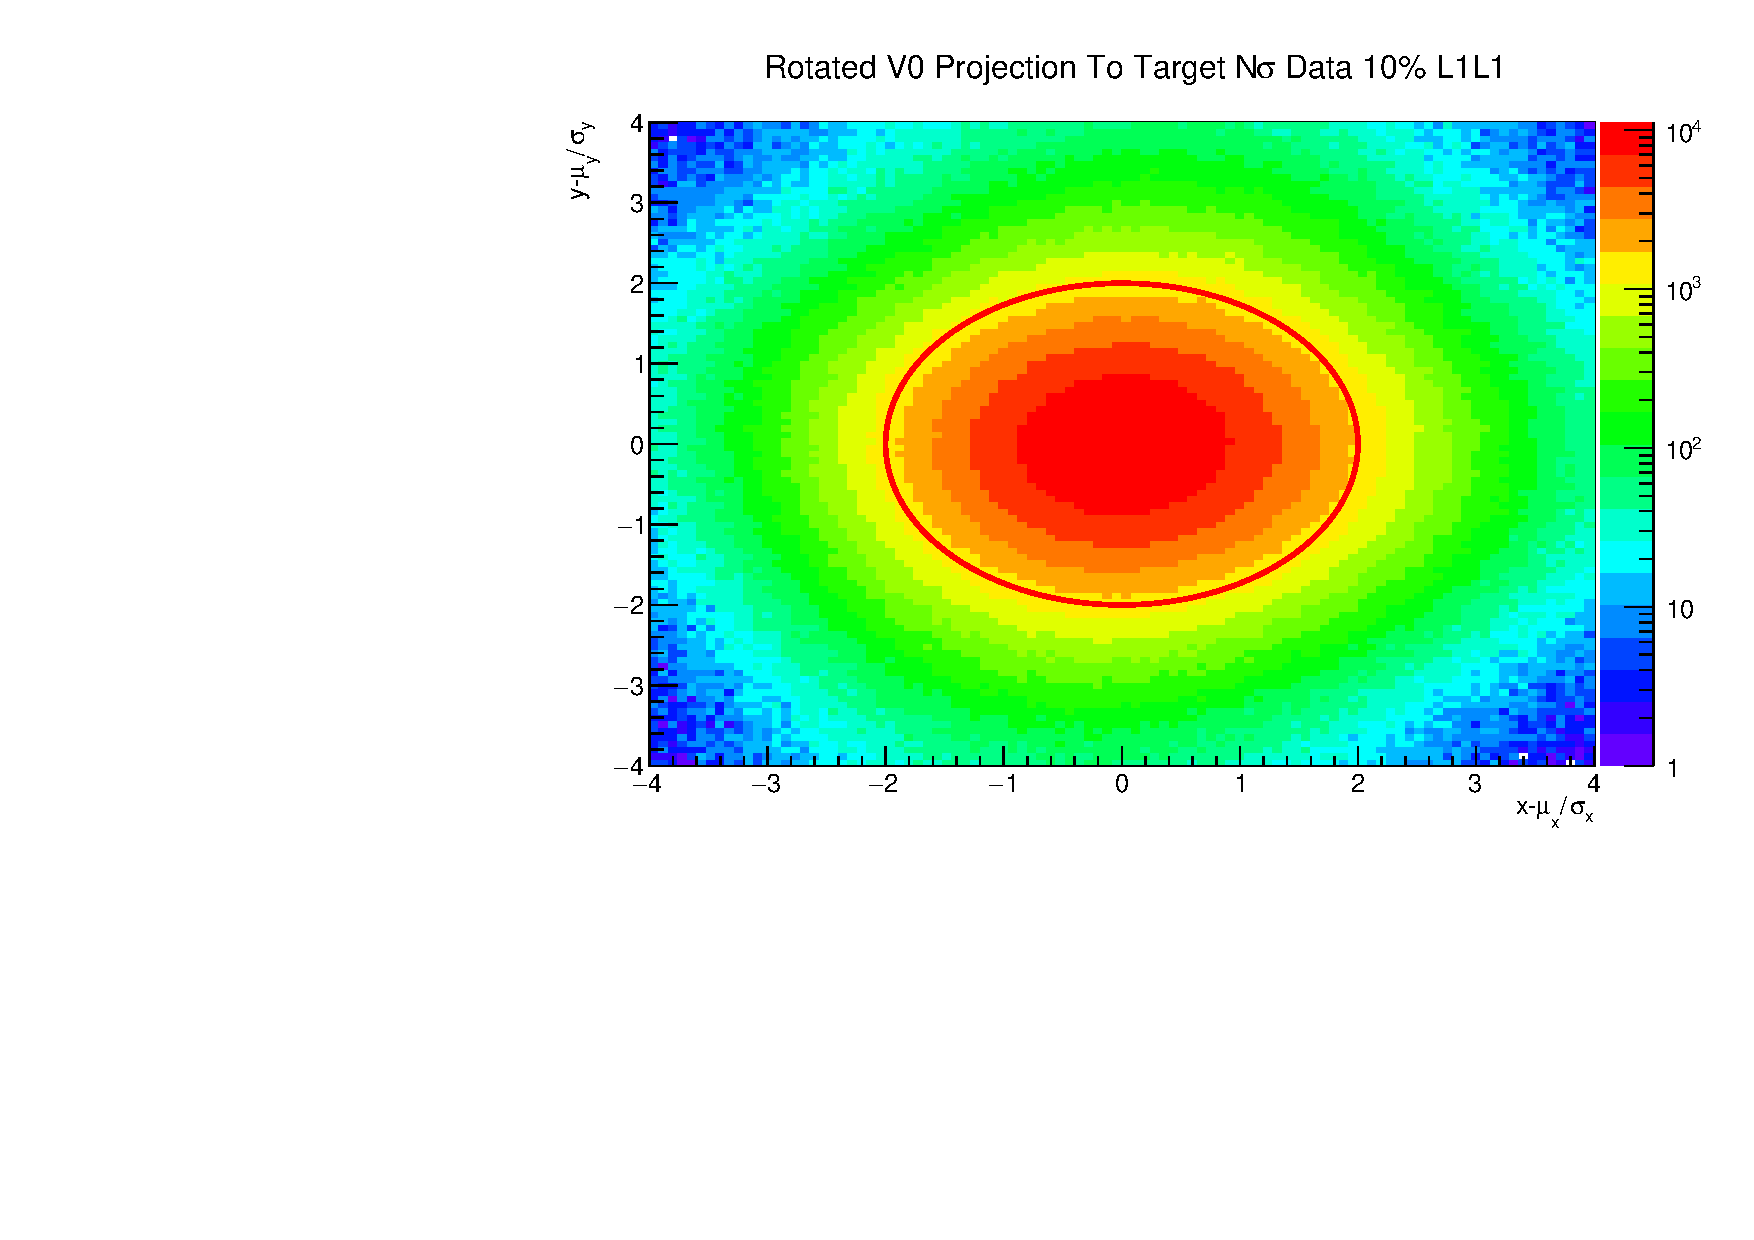
\includegraphics[width=.45\textwidth]{figs/selection/10per_v0proj_L1L1.pdf}
    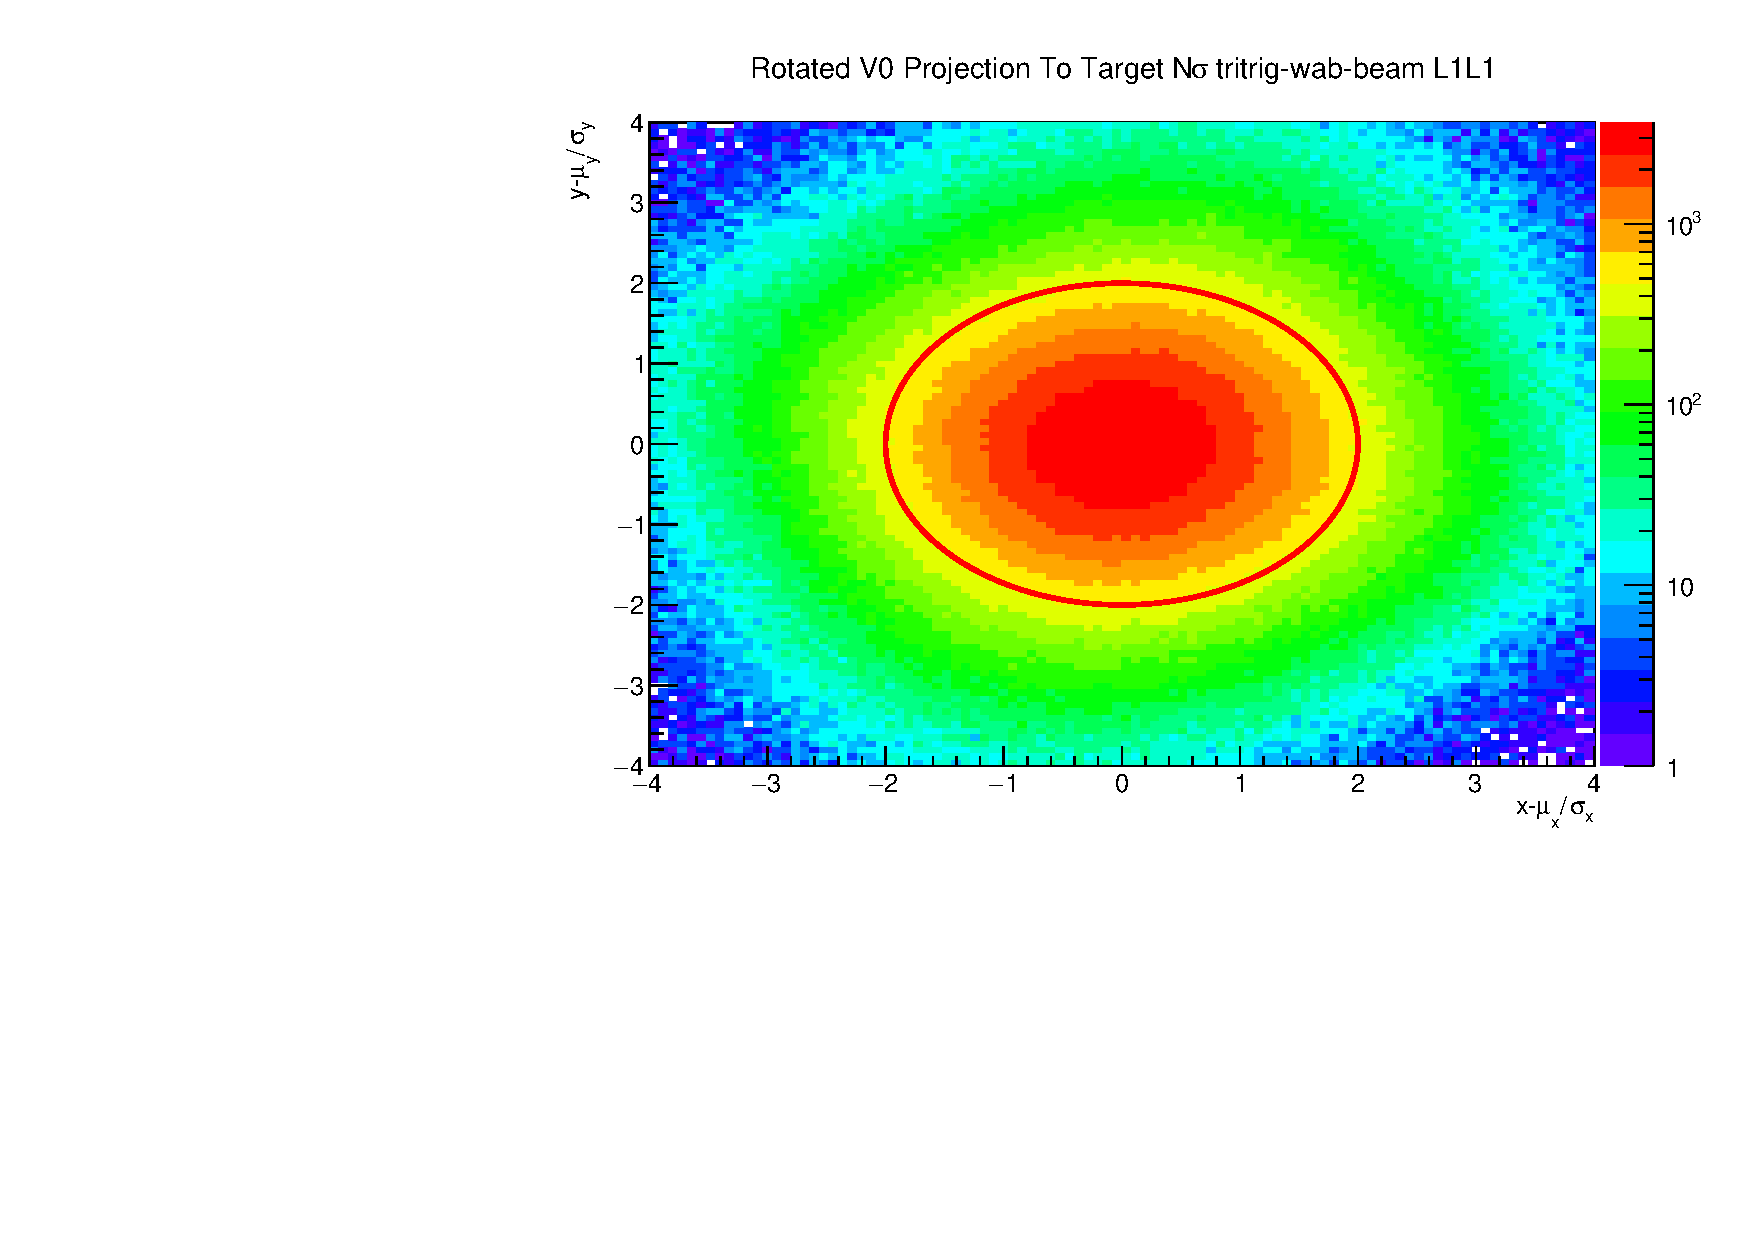
\includegraphics[width=.45\textwidth]{figs/selection/tritrig-wab-beam_L1L1_V0cut.pdf}
    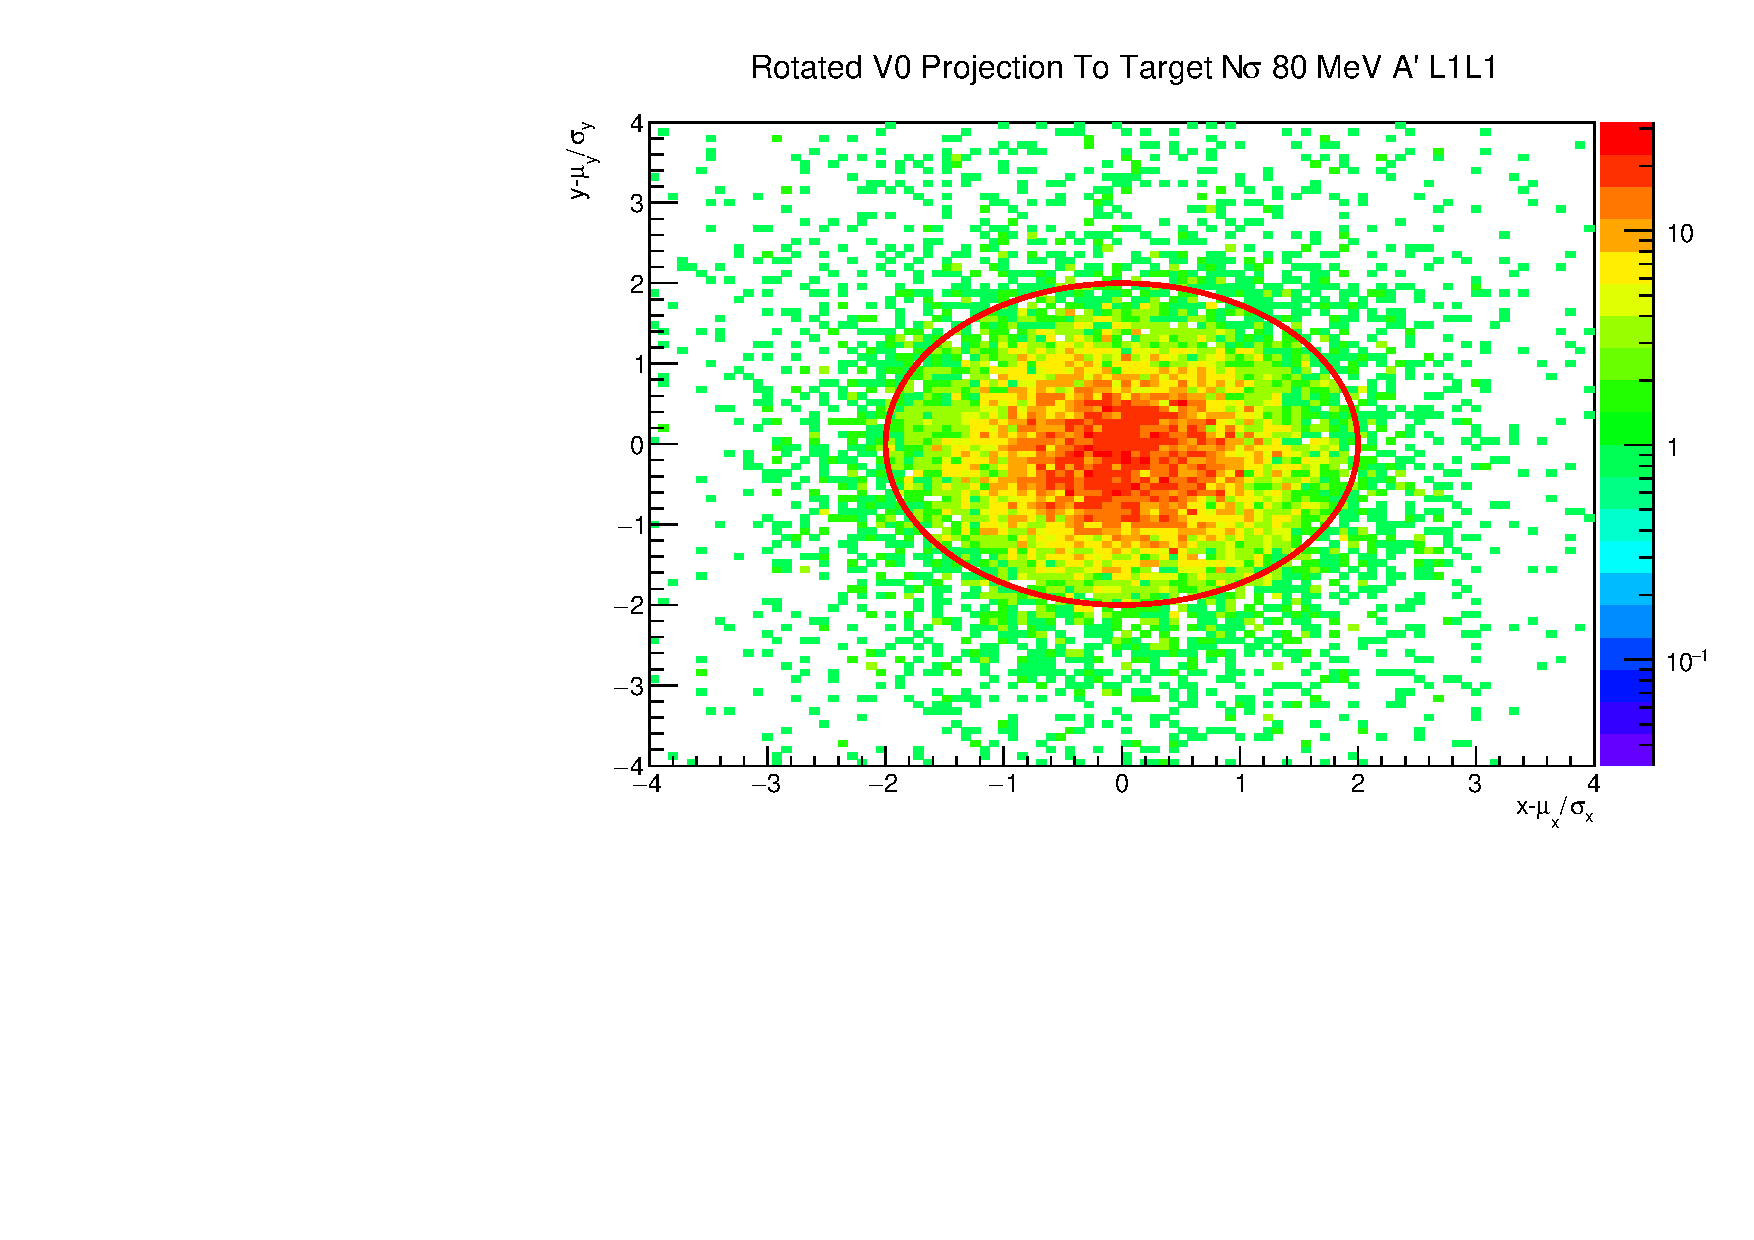
\includegraphics[width=.45\textwidth]{figs/selection/ap-beam_80MeV_L1L1_V0cut.pdf}
    %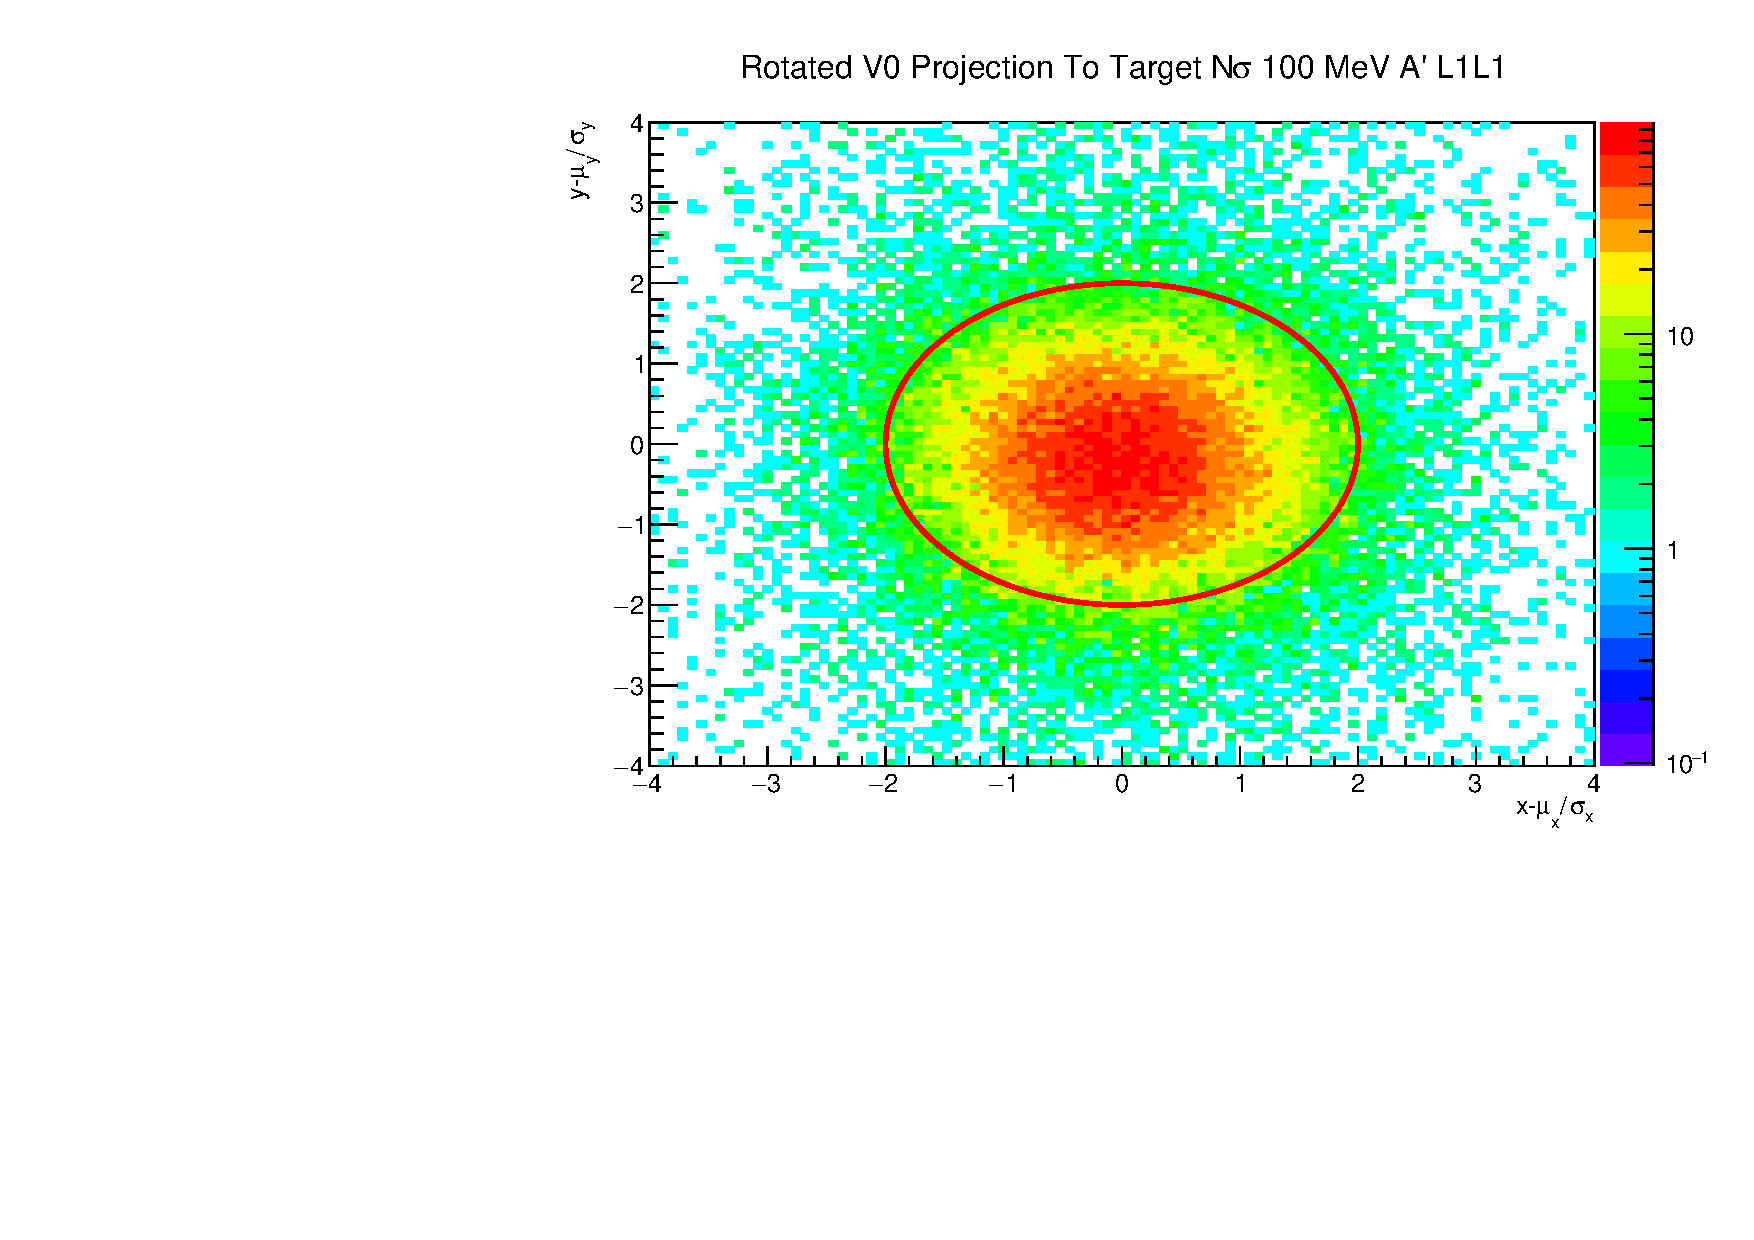
\includegraphics[width=.45\textwidth]{figs/selection/ap-beam_100MeV_L1L1_V0cut.pdf}
    \caption{The V0 projection back to the target significance ($(y-y_{\mu})/\sigma_y$ vs. $(x-x_{\mu})/\sigma_x$) using the rotated coordinates for L1L1 Preselection events for Upper Left: 10\% data, Upper Right: 1\% tritrig-wab-beam, and Bottom: displaced 80 MeV $\aprime$s. %Lower Right: Displaced 100 MeV $A'$. The elliptical cut at $2\sigma$ is shown in red.
    }
    \label{fig:targ_proj_cut}
\end{figure}

\begin{figure}[!ht] 
    \centering
    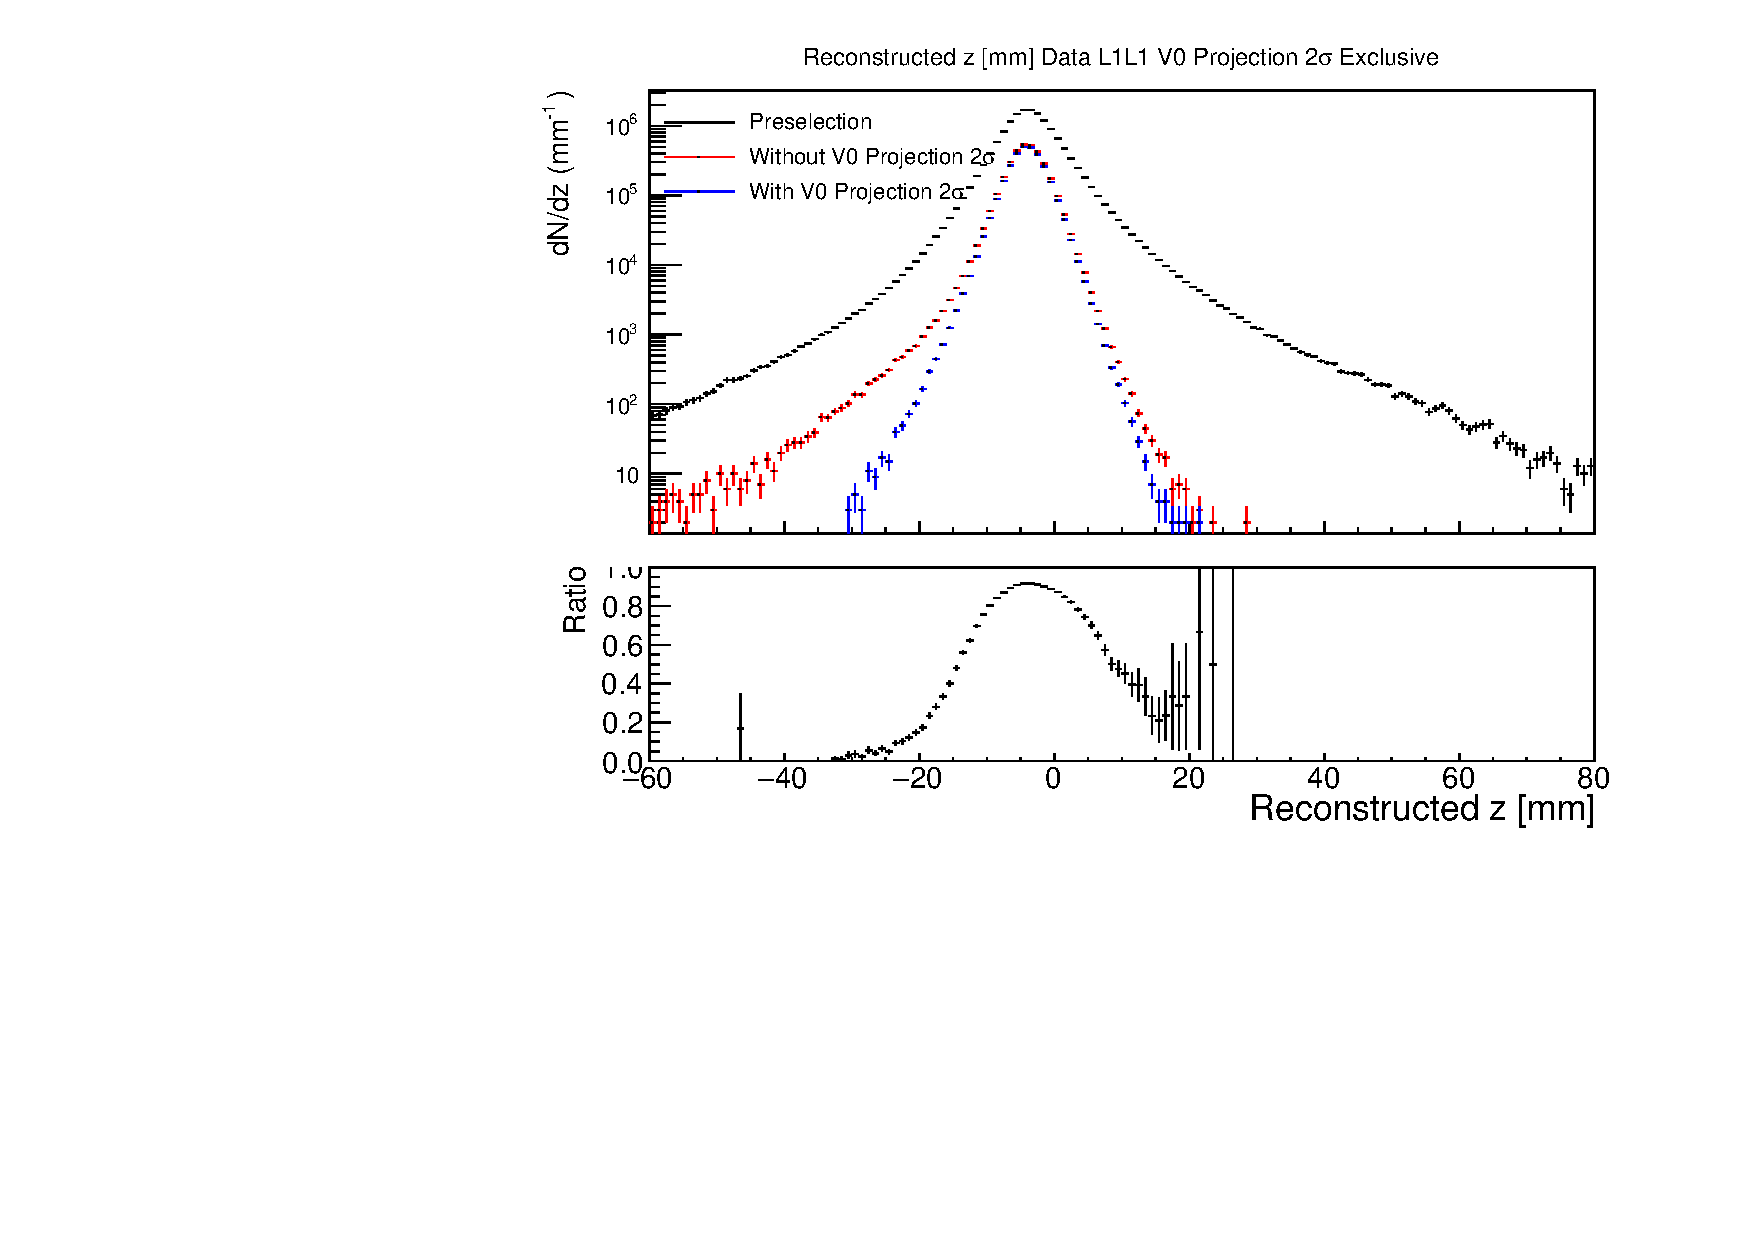
\includegraphics[width=.45\textwidth]{figs/selection/voproj_n_1_z.pdf}
    \includegraphics[width=.45\textwidth]{figs/selection/ap_80MeV_v0proj_n_1_z.pdf}
    \caption{
    	Left: Comparison of preselection, tight cuts, and tight cuts without the V0 projection to the target cut for 10\% Data. Right: Comparison of preselection, tight cuts, and tight cuts without the V0 projection to the target cut for displaced 80 MeV $\aprime$s. These plots show the effectiveness of the V0 projection to the target cut for the L1L1 category.
    }
    \label{fig:v0proj_L1L1}
\end{figure}  

%\begin{figure}[!ht] 
%    \centering
    %\includegraphics[width=.45\textwidth]{images/Selection/voproj_excl_zm.pdf}
%    \includegraphics[width=.45\textwidth]{figs/selection/v0proj_excl_z.pdf}
%    \includegraphics[width=.45\textwidth]{figs/selection/voproj_n_1_z.pdf}
%    \includegraphics[width=.45\textwidth]{figs/selection/v0proj_excl.pdf}
%    \includegraphics[width=.45\textwidth]{figs/selection/ap_80MeV_v0proj_n_1_z.pdf}
%    \includegraphics[width=.45\textwidth]{figs/selection/ap_100MeV_v0proj_n_1_z.pdf}
%    \caption{
%    	Plots showing the effect of the V0 projection to the target cut for the L1L1 category. %Upper Left: Reconstructed Vz vs mass for 10\% Data with all tight cuts except for the V0 projection to the target cut. 
%    	Upper Left: Comparison of VZ distributions for 10\% Data and 100\% tritrig-wab-beam MC for all tight cuts except for the V0 projection to the target cut. Upper Right: Comparison of preselection, tight cuts, and tight cuts without the V0 projection to the target cut for 10\% Data. Middle Left: Comparison of the V0 projection to the target in units of $n_{\sigma}$ for 10\% Data and tritrig-wab-beam MC using all tight cuts except the V0 projection to the target cut. Middle Right: Comparison of preselection, tight cuts, and tight cuts without the V0 projection to the target cut for displaced 80 MeV A's. Bottom: Comparison of preselection, tight cuts, and tight cuts without the V0 projection to the target cut for displaced 100 MeV A's.
%    }
%    \label{fig:v0proj_L1L1}
%\end{figure}  

\clearpage

\textbf{Isolation Cut}

\begin{figure}[t]
    \centering
    \includegraphics[width=.35\textwidth]{figs/selection/isocut_schem.png}
    \includegraphics[width=.45\textwidth]{figs/selection/isocut.png}
    \caption{Left: Example of mis-tracking from a layer 1 bad hit that falsely reconstructs downstream of the target. Right: Geometric picture of the isolation cut comparing the distance between the nearest hit away from the beam $\delta$ and the track longitudinal impact parameter of the track $z0$ where the correct track is in green and the incorrect track found by the tracking algorithm is in red.
    }
    \label{fig:iso_cut}
\end{figure}

%\begin{figure}[t]
%    \centering
%    \includegraphics[width=.45\textwidth]{images/Selection/lcsim_1.png}
%    \includegraphics[width=.45\textwidth]{images/Selection/lcsim_2.png}
%    \caption{A schematic of the linear collider tracking parameters. %http://flc.desy.de/lcnotes/notes/localfsExplorer_read?currentPath=/afs/desy.de/group/flc/lcnotes/LC-DET-2006-004.pdf
%    }
%    \label{fig:track_params}
%\end{figure}

Mis-reconstructed tracks are tracks that contain at least one hit that is not associated with the particle responsible for the majority of other hits of the track. For instance, a track can reconstruct from a real particle trajectory but with an additional hit from a beam electron, recoil electron, photon, or noise hit. This incorrect hit is also called a ``bad hit.'' And when this additional hit is in layer 1 and is closer to the beam than the true hit (or if the true hit doesn't exist), this can falsely reconstruct a downstream vertex, often significantly downstream, that appears signal-like as shown in Fig. \ref{fig:iso_cut}. Often this occurs as a result of scattering in the second layer causing the track to extrapolate to the incorrect hit in layer 1 (often times having a better track quality than a track with the true hit) and occurs at a significant enough rate that it needs to be mitigated.

The isolation cut is performed on tracks, and as discussed in Sec. \ref{sec:coordinates} is complicated by the fact that the coordinate system used for track reconstruction and analysis differ.% the coordinate systems for track reconstruction utilizes perigee parametrization while the analysis uses detector coordinates.

%The isolation cut is performed on tracks, and unfortunately, the coordinate systems for track reconstruction and analysis on HPS are different. In the analysis, as previously stated, the $x$ direction is beam left, the $y$ direction is vertical upwards, and the $z$ direction is the direction of the beam. The tracking coordinates are oriented approximately such that the $x$ direction is the direction of the beam, the $y$ direction is beam left, and the $z$ direction is the vertically upwards. In addition, each track is defined by 5 track parameters - $\Omega$, $d0$, $z0$, $tan \lambda$, and $\phi$ - and are briefly described below and shown in Fig. \ref{fig:track_params}, as well as described in more detail here \textcolor{red}{(cite this paper:)}% http://flc.desy.de/lcnotes/notes/localfsExplorer_read?currentPath=/afs/desy.de/group/flc/lcnotes/LC-DET-2006-004.pdf)}. 

%\begin{enumerate}
%  \item $\Omega$ is the signed curvature of the track (i.e. the inverse of the radius).
%  \item $d0$ is the signed impact parameter in the $xy$ tracking plane. In the HPS detector frame, this translates to the impact parameter along the $x$ (horizontal) direction.
%  \item $z0$ is the tracking $z$ position at the point of closest approach to the reference point. This is the key tracking parameter for the isolation cut. In the HPS detector frame, this approximately corresponds to the impact parameter in the $y$ (vertical) direction.
%  \item $tan \lambda$ is the slope of the straight line in the $sz$ tracking plane. In the HPS detector frame, this translates to the slope of the track $dy/dz$ in the $yz$ plane.
%  \item $\phi$ is the azimuthal angle of the momentum of the particle at point of closest approach to the reference point.
%\end{enumerate}

The isolation cut utilizes a post-reconstruction strategy designed to eliminate high $z$ backgrounds due to mis-tracking from bad hits in layer 1. In particular, tracks that mis-reconstruct the 3D hit in the first layer of the SVT where the hit on track is closer to the beam plane than the true hit can reconstruct a downstream vertex that appears to be signal-like. The isolation cut offers a simple method to test if fitting a track with another hit in layer 1 is more consistent with the track coming from the primary than the secondary vertex without re-running track reconstruction (even if the original track would have better track quality). If the track is more consistent with the primary, the event is eliminated. 

The most basic form of this cut is a simple geometric cut that compares the distance of the next closest hit in the sensor, called the isolation value $\delta$, to the track longitudinal impact parameter $z0$ (tracking $z$ is in the vertical direction $y$ in the detector frame). First, since the track parameter $z0$ is recorded at the origin and the target position is upstream from the origin at $z_{targ}=-4.3$ mm, the value of $z0$ is corrected to the impact parameter at the target $z0_{corr}$ using a simple linear extrapolation of the track state to the target.

%\begin{equation}
%    z0_{corr}=(z0 - z_{targ} \ \frac{P_Y}{P})  \ \mathrm{sign}(P_Y).
%    \label{eq::z0corr}
%\end{equation}

The isolation value $\delta$ is the distance along the measurement direction for each sensor between the 1D cluster hit on track and the next nearest 1D cluster hit in the direction away from the beam plane. By sign convention, $\delta$ is always positive, and the 1D cluster hits closer to the beam plane are not considered since these will reconstruct the vertex further downstream (and we are testing if a track fit with another hit is more consistent with the primary). Furthermore, only the minimum isolation value between the axial and stereo sensor in a given layer is considered.

Comparing this value to the impact parameter, the geometrical condition of the isolation cut is such that, for the track to pass the cut, the isolation value must be greater than the product of the impact parameter and the ratio of the distance between first 2 measurement points and the distance between the second measurement and the primary (i.e. $\frac{z_{L2}-z_{L1}}{z_{L2}-z_{targ}}$). In the case of a layer 1 isolation cut, since the ratio of the distance between layer 2 and layer 1 and layer 2 and the target is about one half, the ratio used in this condition is $\frac{1}{2}$. Otherwise, this ``refitted" track is more consistent with the primary and the event is eliminated. This concept is shown in Figure \ref {fig:iso_cut}, and this condition can be expressed with the following inequality.

\begin{equation}
    \delta + \frac{1}{2}z0_{corr}> 0
    \label{equ:iso_basic}
\end{equation}

%where $\delta$ is the distance between the 1D cluster hit on track and the nearest cluster on the side away from the beam. By sign convention, $\delta$ is always positive, and the clusters closer to the beam are not considered. In addition, only the minimum value of $\delta$ between the axial and stereo sensors is considered. 

It has been shown in the previous displaced vertexing analysis from the 2015 engineering run that this simple geometric cut eliminates a large fraction of high $z$ events due to mis-tracking \cite{adrian2018search}. However, it fails to account for multiple scattering in layer 1. Thus, the high $z$ backgrounds of this nature were not mitigated to the full potential in the previous analysis. In other words, there were high $z$ backgrounds observed in both data and MC that were near the edge of this basic isolation cut, and shifting the cut by even a small amount would have further reduced high $z$ background. Extending the simple geometric cut by incorporating an error on the impact parameter $z0_{corr}$ accounts for the multiple scattering in the tracker.
%In order to further reduce the number of high $z$ events due to mistracking, the isolation cut has been tightened by taking into account multiple scattering effects due to the charged particle traversing L1. 

\begin{figure}[!ht] 
    \centering
    \includegraphics[width=.45\textwidth]{figs/selection/isocut_n_1_z.pdf}
    \includegraphics[width=.45\textwidth]{figs/selection/ap_80MeV_isocut_n_1_z.pdf}
    \caption{
    	Left: Comparison of preselection, tight cuts, and tight cuts without the isolation cut for 10\% Data. Right: Comparison of preselection, tight cuts, and tight cuts without the isolation cut for displaced 80 MeV $\aprime$s. These plots show the effectiveness of the isolation cut for the L1L1 category.
    }
    \label{fig:isocut_L1L1}
\end{figure} 

%\begin{figure}[!ht] 
%    \centering
    %\includegraphics[width=.45\textwidth]{images/Selection/isocut_excl_zm.pdf}
%    \includegraphics[width=.45\textwidth]{figs/selection/isocut_excl_z.pdf}
%    \includegraphics[width=.45\textwidth]{figs/selection/isocut_n_1_z.pdf}
%    \includegraphics[width=.45\textwidth]{figs/selection/isocutele_excl.pdf}
%    \includegraphics[width=.45\textwidth]{figs/selection/isocutpos_excl.pdf}
%    \includegraphics[width=.45\textwidth]{figs/selection/ap_80MeV_isocut_n_1_z.pdf}
%    \includegraphics[width=.45\textwidth]{figs/selection/ap_100MeV_isocut_n_1_z.pdf}
%    \caption{
%    	Plots showing the effect of with and without the isolation cut for the L1L1 category. %Upper Left: Reconstructed Vz vs mass for 10\% Data with all tight cuts except for the isolation cut. 
%    	Upper Left: Comparison of VZ distributions for 10\% Data and 100\% tritrig-wab-beam MC for all tight cuts except for the isolation cut. Upper Right: Comparison of preselection, tight cuts, and tight cuts without the isolation cut for 10\% Data. Middle Left: Electron isolation cut value for 10\% Data and tritrig-wab-beam MC using all tight cuts except the isolation cut. Middle Right: Positron isolation cut value for 10\% Data and tritrig-wab-beam MC using all tight cuts except the isolation cut. Bottom Left: Comparison of preselection, tight cuts, and tight cuts without the isolation cut for displaced 80 MeV A's. Bottom Right: Comparison of preselection, tight cuts, and tight cuts without the isolation cut for displaced 100 MeV A's.
%    }
%    \label{fig:isocut_L1L1}
%\end{figure} 

In order to take multiple scattering into account, the $z0_{corr}$ term in Equation \ref{equ:iso_basic} is modified by adding the estimate of its error at the target position, effectively shifting the value of the isolation cut.

\begin{equation}
    z0_{corr} \longrightarrow z0_{corr} + \Delta z0_{corr}
\end{equation}

%As stated above, in reconstruction the impact parameter $z0$ and error $\Delta z0$ is given with respect to the origin of the reference system. Thus, the error on the impact parameter must also be propagated to the target position. Propagating the error requires the use of the track slope tan$\lambda$ and track curvature $\Omega$ as well as their errors. Assuming the track parameter errors are uncorrelated, $\Delta z0_{corr}$ can simplify to

%\begin{equation}
%    \Delta z0_{corr} = \Delta z0 + |z_{targ}| \ (\Delta tan \lambda + 2 \ |tan \lambda \frac{\Delta \Omega}{\Omega}|)
%    \label{equ:ip_err}
%\end{equation}

%This corrected error at the target results in an increase in error of about 10\% with respect to $\Delta z_{0}$. 

\begin{figure}[t]
    \centering
    \includegraphics[width=.45\textwidth]{figs/selection/isocut_data_z.pdf}
    \includegraphics[width=.45\textwidth]{figs/selection/isocut_mc_puretracks_z.pdf}
    \includegraphics[width=.45\textwidth]{figs/selection/isocut_mc_badtracks_z.pdf}
    \caption{The plots show the reconstructed $z$ vs. the quantity in eq. \ref{equ:iso_final_simple} with preselection and layer 1 requirements. This value combines positrons and electrons for both top and bottom, but only uses the minimum positive isolation value for the axial and stereo pair in layer 1. Upper Left: 10\% Data. Upper Right: 100\% tritrig-wab-beam with only pure tracks (i.e. no mis-tracking). Bottom: 100\% tritrig-wab-beam with only mis-tracking in layer 1. The band structure correlated with reconstructed $z$ in the ``Bad Hits'' MC plot is not present in the ``Pure Tracks'' MC plot, indicating that this is a result of mis-tracking.}
    \label{fig:iso_cut_data}
\end{figure}

%\begin{figure}[t]
%    \centering
%    \includegraphics[width=.45\textwidth]{figs/selection/isocut_mc_puretracks_z.pdf}
%    \includegraphics[width=.45\textwidth]{figs/selection/isocut_mc_badtracks_z.pdf}
%    \caption{Reconstructed $z$ vs. the isolation cut value in eq. \ref{equ:iso_final_simple} for 100\% of the tritrig-wab-beam MC sample with preselection and layer 1 requirements. This isolation cut value combines positrons and electrons for both top and bottom, but only plots the minimum positive isolation value for the axial and stereo pair in layer 1. The left plot only selects tracks that match to the same MCParticle, while the plot on the right only selects V0 particles that contain either an $e^+$ or $e^-$ track that have an incorrect layer 1 hit.}
%    \label{fig:iso_cut_mc}
%\end{figure}

Typically, the errors of the impact parameter at the target are $\sim$0.1 mm. In order to take into account large scatters in the L1 material, the isolation cut takes into account the errors in the track extrapolation on a track-by-track basis by shifting the cut value up to a specified $n_{\sigma}$ on $z0$ leading to a final equation for the isolation cut given by 

\begin{equation}
    \delta + \frac{1}{2} \ (z0_{corr} - n_{\sigma} \ \Delta z0_{corr})> 0
    \label{equ:iso_final_simple}
\end{equation}

The last step in finalizing the isolation cut is to select the number $n_{\sigma}$ to use in the cut. In general, the signal efficiency is fairly insensitive to this value (since $\Delta z0_{corr} \sim 100 \mu$m). % as shown in Fig. \ref{fig:floatcut_iso_L1L1} where n$\sigma$ is varied as 2.5, 3, and 3.5. 
A reasonable value on the error is $3\sigma$ which eliminates all high $z$ background due to mis-tracking according to MC (a simple study analyzing the signal efficiency shows that the result is generally independent between the range of $n_{\sigma}=2.5$ to $n_{\sigma}=3.5$). The effect of the cut is qualitatively demonstrated with $n-1$ plots comparing all cuts and all cuts except of the isolation cut. As shown in Fig. \ref{fig:isocut_L1L1}, the cut eliminates a large number of high $z$ events with minimal impact on signal efficiency (though with a slight $z$ dependence due to the geometry of the isolation cut). %The effect of the cut on 10\% data, 100\% tritrig-wab-beam, and 80 MeV and 100 MeV displaced $A'$s is shown in Fig. \ref{fig:isocut_L1L1}.

%For the tight vertex selection, only tracks that pass the requirement $\iota_{trk} > 0$ are considered.  

In order to better understand the effect of the isolation cut, it is important to see its effect on both good tracks (tracks in which all hits on track are a result of its truth match) and bad tracks (or mis-tracks, those with at least one bad hit) which can be determined by truth-matched tracks in MC as described in Sec. \ref{sec:tracktruth}. For preselected events with layer 1 hits, the reconstructed $z$ positions vs the quantity in eq. \ref{equ:iso_final_simple} for 10\% of the data and 100\% the tritrig-wab-beam MC sample separated into good and bad tracks are shown in Fig. \ref{fig:iso_cut_data}. The ``Bad Hit'' MC plot shows a band structure correlated with reconstructed $z$ that is not present in the ``Pure Tracks'' plot, indicating that this structure is due to mis-tracking. Since data contains a mix of both good and bad tracks (which are of course impossible to separate without truth information), the data plot is the sum of the two MC plots, where the ``bad hit'' structure is visible. The cut value at 0 from Eq. \ref{equ:iso_final_simple} eliminates the high $z$ events in this band due to mis-tracking. %and displaced $A'$ MC at two different mass points are shown in Fig. \ref{fig:iso_cut_data}, Fig. \ref{fig:iso_cut_mc}, and Fig. \ref{fig:iso_cut_ap}, respectively. 

Finally, a comparison of the reconstructed $z$ distribution for 100\% tritrig-wab-beam for V0 particles with 100\% pure $e^+$ and $e^-$ tracks and V0 particles with at least one $e^+$ or $e^-$ track with a bad hit in L1 is shown in Fig. \ref{fig:iso_good_bad}. For tritrig-wab-beam, 98.8\% of the V0 particles have 100\% pure tracks for both $e^+$ and $e^-$ tracks while 0.95\% of the V0 particles have either $e^+$ or $e^-$ with a bad L1 hit. The remaining fraction of V0 particles have either an $e^+$ or $e^-$ bad hit in a layer other than L1 (with good hits in L1) or have no track to truth match for either the $e^+$ or $e^-$ particle. Even though pure tracks make up most of the dataset, a large number of high $z$ events are a result of mis-tracking but can be sufficiently mitigated.

The isolation cut is not sensitive to sensor inefficiencies as it has been developed under the assumption that a real 1-D hit has been reconstructed. Therefore tracks that are reconstructed with an incorrect 1-D hit because the true hit has failed the reconstruction cannot be eliminated by this cut. The possible effects of hit efficiencies on high $z$ backgrounds is discussed in more detail in Sec. \ref{sec:highz}.

%\begin{figure}[t]
%    \centering
%    \includegraphics[width=.45\textwidth]{figs/selection/isocut_ap80MeV_isocut_z.pdf}
%    \includegraphics[width=.45\textwidth]{figs/selection/isocut_ap100MeV_isocut_z.pdf}
%    \caption{Reconstructed $z$ vs. the isolation cut value in eq. \ref{equ:iso_final_simple} for an 80 MeV (left) and 100 MeV (right) displaced $A'$ with preselection and layer 1 requirements. This isolation cut value combines positrons and electrons for both top and bottom, but only plots the minimum positive isolation value for the axial and stereo pair in layer 1.}
%    \label{fig:iso_cut_ap}
%\end{figure}

\begin{figure}[t]
    \centering
    \includegraphics[width=.85\textwidth]{figs/selection/isocut_goodbad_z.pdf}
    \caption{A comparison of the reconstructed $z$ distribution for V0 particles with 2 tracks that have all the hits matched to an MC particle (blue) and those with either an $e^+$ or $e^-$ track with a bad layer 1 hit. Mis-tracking results in a large number of high $z$ events.}
    \label{fig:iso_good_bad}
\end{figure}

\clearpage

\textbf{Impact Parameters}

For signal, a true displaced vertex will have large impact parameters ($z0$) in the vertical direction for both electron and positron tracks. Furthermore, these impact parameters are correlated with $z$, where both electron and positron impact parameters increase with increasing $z$ in well-defined bands. For prompt background that reconstructs at large $z$, this is usually not the case. Instead, it is possible for one particle to have a large scatter away from the beam plane (and thus a large impact parameter) and the corresponding particle to either be consistent with the primary or have a smaller impact parameter than is expected from signal. With a cut on impact parameter on both $\epem$ tracks, such backgrounds can be eliminated. This concept is illustrated in Fig. \ref{fig:z0_schem}.

\begin{figure}[t]
    \centering
    \includegraphics[width=.95\textwidth]{figs/selection/Z0_schem.png}
    \caption{Left: Prompt background that falsely reconstructs at a large $z$ due to an $e^-$ particle with a large scatter away from the beam plane in layer 1 of the SVT. The corresponding $e^+$ does not have a large scatter and the track points back near the primary. A cut on the impact parameter can eliminate such backgrounds. Right: A true displaced vertex will have a large impact parameter for both $\epem$ pairs that is correlated with reconstructed $z$.}
    \label{fig:z0_schem}
\end{figure}

%\begin{figure}[t]
%    \centering
%    \includegraphics[width=.45\textwidth]{images/Selection/z0cut_intercept.png}
%    \includegraphics[width=.45\textwidth]{images/Selection/z0cut_slope.png}
%    \caption{Left: The $y-$intercept for a linear fit in z0 vs reconstructed $z$ at various mass points. Each For simplicity, the range is fit with a constant and used as an input to Eq: \ref{equ:z0_cut} ($a_{+}(m)=a_{-}(m)=a$) . Right: The slope for a linear fit in z0 vs reconstructed $z$ as a function of mass for tracks in the top volume of the SVT. The range is fit using Eq. \ref{equ:z0_cut_m}.
%    \textcolor{red}{These plots are ugly, but I can replace them in the future if necessary.}}
%    \label{fig:z0_slope}
%\end{figure}

\begin{figure}[t]
    \centering
    \includegraphics[width=.45\textwidth]{figs/selection/data_L1L1_80MeV_IP.pdf}
    \includegraphics[width=.45\textwidth]{figs/selection/data_L1L1_100MeV_IP.pdf}
    \includegraphics[width=.45\textwidth]{figs/selection/80MeV_L1L1_IP.png}
    \includegraphics[width=.45\textwidth]{figs/selection/100MeV_L1L1_IP.png}
    \caption{Impact parameter vs. reconstructed $z$ for different mass values of 10\% data and $\aprime$s in the L1L1 category. The red lines indicate the impact parameter cut at the specified mass value. Upper Left: 10\% data in mass range 75-85 MeV. Upper Right: 10\% data in the mass range 95-105 MeV. Lower Left: 80 MeV Displaced $A'$s. Lower Right: 100 MeV Displaced $\aprime$s.}
    \label{fig:z0_plots}
\end{figure}

In order to fully utilize the impact parameters as a method to discriminate between background and signal, this cut is performed as a function of reconstructed $z$ in order to fit the signal bands shown in the $z0$ vs. reconstructed $z$ plots of Fig. \ref{fig:z0_plots}. This figure also shows the same plot in 10\% of the data with preselection and layer 1 requirements. This correlation in signal is approximately linear for the masses of interest (which can be seen for 80 MeV and 100 MeV), so there is a requirement that the cut is linear in $z$.

\begin{equation}
    z0_+(m,z) > a_{+}(m) + b_{+}(m) \ z \ \mathrm{or} \
    z0_-(m,z) < a_{-}(m) + b_{-}(m) \ z 
    \label{equ:z0_cut}
\end{equation}

Both the electron and positron are required to satisfy this condition of being above or below one of these lines, respectively. The difference in slope between the positive and negative functions ($b_{+}$ and $b_{-}$) is large enough such that they are different constants. Since the opening angle of an $\aprime$ is mass-dependent, the slopes of these cuts (and also the $z$-independent term) also depends on mass. Thus, the constants $a_{\pm}$ and  $b_{\pm}$ must be parametrized as a function of mass.

In order to obtain these constants for a given $A'$ mass, a linear fit to the inner bands of the $z0$ vs $z$ distributions, combining both the electron and positron distributions, is performed for a single $A'$ mass. Specifically, the $z0$ distributions are sliced in overlapping bins of $z$ and the point at which a certain fraction of the signal will be eliminated on the side closer to the beam plane (i.e. the ``inner'' portion of the $z0$ distribution) is determined. This fraction of the signal that is chosen to be eliminated is a tuneable parameter denoted as $\alpha$. This defines the constants $a_{\pm}$ and $b_{\pm}$ at a specific mass. This process is repeated for each mass point in the range 60 MeV - 150 MeV and a linear fit using the same $\alpha$ is performed at each mass. 

As stated previously, each of these parameters that are linear in $z$ must be parametrized as a function of mass. The fits show that the $a_{\pm}$ parameter is generally within 25 $\mu$m across all masses including both the positive and negative fit. Thus, this parameter is fit to a constant across all masses such that $a_{+}=a_{-}=a$. The relationship between the mass and the slope is non-linear and increases approximately asymptotically with increasing with mass.

\begin{equation}
    b_{\pm}(m) = b_{0\pm} + \frac{b_{1\pm}}{m}
    \label{equ:z0_cut_m}
\end{equation}

%These two assumptions are justified in Fig. \ref{fig:z0_slope}. 
Finally, the cut equations can be summed up with 5 parameters $a$, $b_{\pm}$, and $b_{\pm}$ that are set with a single tuneable parameter $\alpha$.

\begin{equation}
    z0_+(m,z,\alpha) > a(\alpha) + b_{0+}(\alpha) \ z \ +  b_{1+}(\alpha) \frac{z}{m} \ \mathrm{or} \
    z0_-(m,z,\alpha) < a(\alpha) + b_{0-}(\alpha) \ z \ +  b_{1-}(\alpha) \frac{z}{m} 
    \label{equ:z0_cut_final}
\end{equation}

In addition, since there is a mass-dependent target position for data (but not for MC) as shown in Fig. \ref{fig:mass_slice}, and these constants must be determined from MC, the reconstructed $z$ for this cut in data is shifted by a value $dz$ determined by the difference in fitted mean between 10\% data and MC preselection.

\begin{equation}
    dz = -0.377 + 13.79 m - 55.84 m^2 + 84.00 m^3
    \label{equ:meanz_pre}
\end{equation}

In addition to the shift in $z$, there are shifts in the $y$-direction due to changing beam conditions. The beam position in $y$ can shift by as much as 50 $\mu$m which can have a significant impact on the signal efficiency of the impact parameter cut. To mitigate this effect, a run-dependent beam $y$ position is utilized in the same way that the V0 projection back to the target is run-dependent.

%Next, the parameter $\alpha$ must be chosen. Table \ref{tab:IP_L1L1_80} and Table \ref{tab:IP_L1L1_100} show the number of high $z$ backgrounds (past the $z_{cut}$ of the 10\% of the data) in 10\% of the data, 100\% of the tritrig-wab-beam sample, and x3 tritrig sample as well as the efficiency for 80 MeV and 100 MeV displaced $A's$. Based on this data, $\alpha=15\%$ was selected as it eliminates a significant amount of background in all categories, with minimal affect on signal efficiency. At this $\alpha$, the value of the 5 parameters are: $a=-2.018e10^{-1}$, $b_{0+}=5.199e10^{-2}$,  $b_{1+}=-2.301e10^{-3}$,  $b_{0-}=4.716e10^{-2}$,  and $b_{1-}=-1.086e10^{-3}$. The effect of floating the cut about different values of $\alpha$ is shown in Fig. \ref{fig:floatcut_ip_L1L1}. The effect of the impact parameter cut is shown in Fig. \ref{fig:ip_L1L1}.

Next, the tuneable parameter $\alpha$ must be chosen. A simple study showed that the final result is generally independent of $\alpha$ in the range 10\% - 20\%, and $\alpha=15\%$ was selected. At this $\alpha$, the value of the 5 parameters are: $a=-0.2018$, $b_{0+}=5.199 \times 10^{-2}$,  $b_{1+}=-2.301 \times 10^{-3}$,  $b_{0-}=4.716 \times 10^{-2}$,  and $b_{1-}=-1.086 \times 10^{-3}$. In order to evaluate the qualitative effectiveness of the impact parameter cut, $n-1$ plots are shown in Fig. \ref{fig:ip_L1L1} in which the final selection is compare with all tight cuts with the exception of the impact parameter cut. A large number of high $z$ events and events on the tail are eliminated with minimal impact on the signal efficiency (though with some $z$-dependence due to a small non-linearity in the $z0$ vs reconstructed $z$ fits for signal).

\begin{figure}[!ht] 
    \centering
    \includegraphics[width=.45\textwidth]{figs/selection/ip_n_1_z.pdf}
    \includegraphics[width=.45\textwidth]{figs/selection/ap_80MeV_ip_n_1_z.pdf}
    \caption{
    	Left: Comparison of preselection, tight cuts, and tight cuts without the impact parameter cut for 10\% Data. Right: Comparison of preselection, tight cuts, and tight cuts without the impact parameter cut for displaced 80 MeV $\aprime$s. These plots showing the effect of with and without the impact parameter cut for the L1L1 category.
    }
    \label{fig:ip_L1L1}
\end{figure} 

%\begin{figure}[!ht] 
%    \centering
    %\includegraphics[width=.45\textwidth]{images/Selection/ip_excl_zm.pdf}
%    \includegraphics[width=.45\textwidth]{figs/selection/ip_excl_z.pdf}
%    \includegraphics[width=.45\textwidth]{figs/selection/ip_n_1_z.pdf}
%    \includegraphics[width=.45\textwidth]{figs/selection/z0ele_excl.pdf}
%    \includegraphics[width=.45\textwidth]{figs/selection/z0pos_excl.pdf}
%    \includegraphics[width=.45\textwidth]{figs/selection/ap_80MeV_ip_n_1_z.pdf}
%    \includegraphics[width=.45\textwidth]{figs/selection/ap_100MeV_ip_n_1_z.pdf}
%    \caption{
%    	Plots showing the effect of with and without the impact parameter cut for the L1L1 category. %Upper Left: Reconstructed Vz vs mass for 10\% Data with all tight cuts except for the impact parameter cut. 
%    	Upper Left: Comparison of VZ distributions for 10\% Data and 100\% tritrig-wab-beam MC for all tight cuts except for the impact parameter cut. Top Right: Comparison of preselection, tight cuts, and tight cuts without the impact parameter cut for 10\% Data. Middle Left: Electron track $z0$ for 10\% Data and tritrig-wab-beam MC using all tight cuts except the impact parameter cuts. Middle Right: Positron track $z0$ for 10\% Data and tritrig-wab-beam MC using all tight cuts except the impact parameter cuts. Bottom Left: Comparison of preselection, tight cuts, and tight cuts without the impact parameter cut for displaced 80 MeV A's. Bottom Right: Comparison of preselection, tight cuts, and tight cuts without the impact parameter cut for displaced 100 MeV A's.
%    }
%    \label{fig:ip_L1L1}
%\end{figure} 

\clearpage

\textbf{Radiative Cut}

%\begin{figure}[t]
%    \centering
%    \includegraphics[width=.45\textwidth]{images/Selection/MinvPsum_WitmPSumMinCut_Data.pdf}
%    \caption{Invariant mass vs the momentum sum of a trident sample. The red starts are the optimal momentum sum in slices of mass based on $sig/\sqrt(sig+bck)$ where radiative tridents are signal and tridents are background. Above 60 MeV, the lower mass bound of interest for the displaced vertex search, the optimal value is a momentum sum of about 2.0 GeV.}
%    \label{fig:radcut}
%\end{figure}

As stated previously, the kinematics of $\aprime$s are such that the recoil electron is generally soft while $\aprime$s take most of the beam energy (i.e. have a large $x=E_{A'}/E_{beam}$). Thus, only V0s with momentum near the beam energy are selected, and a minimum V0 momentum cut (in addition to the maximum V0 momentum cut from preselection), the so-called radiative cut, is implemented. %Since radiative tridents have identical kinematics to A's, this cut can be optimized based on radiative trident kinematics against Bethe-Heitler tridents and wabs. And because this is true regardless of whether of not A's are prompt or displaced, it can be optimized in a similar method to the resonance search. 

%The resonance search uses the ratio $sig/\sqrt(sig+bck)$ where the signal expectation comes from radiative tridents and the total expectation comes from the sum of tridents and wabs. The optimum value is generally insensitive to the cut value between the momentum sum ranges from 1.6 GeV to 2.2 GeV, and was found to be 1.88 GeV across all mass ranges. The value of 1.9 GeV was selected for convenience for the resonance search.

%There are two key differences between the resonance search and the displaced vertex search with respect to the radiative cut. The first is the fact that the search for displaced vertices is in a low background region, thus the same ratio doesn't necessarily apply. %However, one can assume that for background due to multiple scattering from prompt processes (e.g. QED tridents), this ratio will be approximately the same to first order even in the low background region. And since $A'$s have identical kinematics to radiative tridents, this method of justifying the radiative cut in a similar manner to the resonance search is a valid approximation.
%Secondly, there is a mass-dependence for this cut optimization shown in Fig. \ref{fig:radcut} which skews the optimization for this figure of merit toward low mass (40 GeV - 60 GeV) and favors a looser radiative cut. For the displaced vertex search with a 2.3 GeV beam energy, the mass range of interest begins at \~60 MeV, which has an optimal value at around 2.0 GeV. %Thus, radiative cut is placed at 2.0 GeV for the displaced vertex search. 

%However, in a low background region, the ratio $sig/\sqrt(sig+bck)$ may not be a sufficient figure of merit for cut optimization. As a better figure of merit, one can use ratio $sig/bck$. In order to provide sufficient statistics for the background term, the entire mass range of interest is used for the background (from 50 MeV - 150 MeV). For this exercise, there are typically 15-20 background events, and a new $z_{cut}$ is fit for each $x_{cut}$ point. It is an assumption that the entire mass range is representative of each individual mass slice. These results for two signal points are shown in Fig. \ref{fig:radcut} and a radiative cut of 1.85 GeV ($x\approx 0.8E_{beam}$) is selected.

The figure of merit used to tune the radiative cut is the optimal ratio of the signal to background in the same way the V0 projection to the target cut was tuned. In order to provide sufficient statistics for the background term, the entire mass range of interest is used for the background (from 50 MeV - 150 MeV). It is an assumption that the entire mass range is representative of each individual mass slice. The results show that in general the ratio signal to background is insensitive between the minimum V0 momentum cut ranges of $1.7-2.0$ GeV; however, this figure of merit peaks at about 1.85 GeV ($x\approx 0.8E_{beam}$). The radiative cut is selected to be at this value. The effectiveness of the radiative cut is evaluated qualitatively by $n-1$ plots on 10\% of the data and an 80 MeV displaced $\aprime$ in which the final selection is compared to the final selection  without the radiative cut. These plots show a significant reduction in events on the tail and high $z$ events for 10\% of the data with minimal impact on the signal and are shown in Fig. \ref{fig:v0p_L1L1}. % while the effect of floating the cut value about its nominal value is shown in Fig. \ref{fig:floatcut_v0p_L1L1}.

\begin{figure}[!ht] 
    \centering
    \includegraphics[width=.45\textwidth]{figs/selection/v0p_n_1_z.pdf}
    \includegraphics[width=.45\textwidth]{figs/selection/ap_80MeV_vop_n_1_z.pdf}
    \caption{
    	Left: Comparison of preselection, tight cuts, and tight cuts without the V0 momentum cut for 10\% Data. Right: Comparison of preselection, tight cuts, and tight cuts without the V0 momentum cut for displaced 80 MeV $\aprime$s. These plots show the effect of the V0 momentum cut for the L1L1 category.
    }
    \label{fig:v0p_L1L1}
\end{figure}  

The complete tight cutflow for the L1L1 category is shown in Fig. \ref{fig:tightcutflow_L1L1}. %A table of the effect of each tight cut in the L1L1 category for data and different MC components is shown in Table \ref{tab:cutflowL1L1}.

%\begin{figure}[!ht] 
%    \centering
    %\includegraphics[width=.45\textwidth]{images/Selection/v0p_excl_zm.pdf}
%    \includegraphics[width=.45\textwidth]{figs/selection/v0p_excl_z.pdf}
%    \includegraphics[width=.45\textwidth]{figs/selection/v0p_n_1_z.pdf}
%    \includegraphics[width=.45\textwidth]{figs/selection/v0p_excl.pdf}
%    \includegraphics[width=.45\textwidth]{figs/selection/ap_80MeV_vop_n_1_z.pdf}
%    \includegraphics[width=.45\textwidth]{figs/selection/ap_100MeV_vop_n_1_z.pdf}
%    \caption{
%    	Plots showing the effect of with and without the V0 momentum cut for the L1L1 category. %Upper Left: Reconstructed Vz vs mass for 10\% Data with all tight cuts except for the V0 momentum cut.
%    	Upper Left: Comparison of VZ distributions for 10\% Data and 100\% tritrig-wab-beam MC for all tight cuts except for the V0 momentum cut. Upper Right: Comparison of preselection, tight cuts, and tight cuts without the V0 momentum cut for 10\% Data. Middle Left: Comparison of the V0 momentum for 10\% Data and tritrig-wab-beam MC using all tight cuts except the V0 momentum cut. Middle Right: Comparison of preselection, tight cuts, and tight cuts without the V0 momentum cut for displaced 80 MeV A's. Bottom: Comparison of preselection, tight cuts, and tight cuts without the V0 momentum cut for displaced 100 MeV A's.
%    }
%    \label{fig:v0p_L1L1}
%\end{figure}  


%\begin{table}[t]
%\centering
%\tabcolsep=0.09cm
%\begin{tabular}{lrlrlrlrl}

% \hline
%                                         &        data & $\epsilon_{tot}$   &    tridents & $\epsilon_{tot}$   &   WAB & $\epsilon_{tot}$   &    AP & $\epsilon_{tot}$   \\
%\hline
% Preselection                                 & - & --                 & - & --                 & - & --                 & - & --                 \\
% L1L1 + L2 Requirements                           & - & -              & 0           & 0.0                &     0 & 0.0                &     0 & 0.0                \\
% $V_0$ Projection to Target  $<2\sigma$      & - & -               & - & -              & - & -              & - & -              \\
% $V_{0p}>2.0$GeV & - & -               & - & -              & - & -              & - & -              \\
% Isolation Cut           & - & -              & - & -              & - & -              & - & -              \\
% Impact Parameter Cut           & - & -              & - & -              & -              & - & -              \\

%\hline

%\hline
%\end{tabular}
%\caption{Table showing the efficiency of each cut on 10\% of the 2016 data sample and on MC simulation for tridents,  WABs and 80 MeV $A'$ displaced samples for the L1L1 category. \textcolor{red}{TODO: Update the cuts and numbers}}
%\label{tab:cutflowL1L1}
%\end{table}

\begin{figure}[!ht] 
    \centering
    \includegraphics[width=.45\textwidth]{figs/selection/datatightcutflowL1L1_vz.pdf}
    \includegraphics[width=.45\textwidth]{figs/selection/mctightcutflowL1L1_vz.pdf}
    \includegraphics[width=.45\textwidth]{figs/selection/ap_80MeV_tightcutflowL1L1.pdf}
    %\includegraphics[width=.45\textwidth]{figs/selection/datatightcutflowL1L1_mass.pdf}
    %\includegraphics[width=.45\textwidth]{figs/selection/mctightcutflowL1L1_mass.pdf}
    %\includegraphics[width=.45\textwidth]{figs/selection/datatightcutflowL1L1_p.pdf}
    %\includegraphics[width=.45\textwidth]{figs/selection/mctightcutflowL1L1_p.pdf}
    \caption{
    	Upper Left: The tight cutflow for 10\% of the data in the L1L1 category. Upper Right: The tight cutflow of the full tritrig-wab-beam sample in the L1L1 category. Bottom: The tight cutflow for 80 MeV displaced $\aprime$s in the L1L1 category. %Lower Left: Comparison of 80 MeV displaced A's for before and after multiple V0 events are removed. Lower Right: Comparison of 100 MeV displaced A's for before and after multiple V0 events are removed.
    }
    \label{fig:tightcutflow_L1L1}
\end{figure} 

\clearpage

\textbf{Selecting Single V0s}

%The tight cutflow for the L1L1 category is shown in Fig. \ref{fig:tightcutflow_L1L1}. A table of the effect of each tight cut in the L1L1 category for data and different MC components is shown in Table \ref{tab:cutflowL1L1}. % and the effect on the reconstructed $z$ vs mass 2D plots are shown in Fig. \ref{fig:L1L1_n_1}.

%\begin{figure}[!ht] 
%    \centering
%    \includegraphics[width=.45\textwidth]{images/Selection/data_L1L1_tight_vz_mass.pdf}
%    \includegraphics[width=.45\textwidth]{images/Selection/voproj_excl_zm.pdf}
%    \includegraphics[width=.45\textwidth]{images/Selection/uncChisq_excl_zm.pdf}
%    \includegraphics[width=.45\textwidth]{images/Selection/v0p_excl_zm.pdf}
%    \includegraphics[width=.45\textwidth]{images/Selection/isocut_excl_zm.pdf}
%    \includegraphics[width=.45\textwidth]{images/Selection/ip_excl_zm.pdf}
%    \caption{
%    	Reconstructed $z$ vs mass for 10\% of the data shown for all tight cuts except for the specified cut in the L1L1 category. Upper Left: All tight cuts for L1L1. Upper Right: No V0 projection cut. Middle Left: No tighter vertex quality requirement. Middle Right: No V0 momentum cut (radiative cut). Lower Left: No isolation cut. Lower Right: No impact parameter cut.
%    }
%    \label{fig:L1L1_n_1}
%\end{figure} 

%\begin{figure}[!ht] 
%    \centering
%    \includegraphics[width=.45\textwidth]{figs/selection/tightcutflowL1L1.pdf}
%    \includegraphics[width=.45\textwidth]{figs/selection/tightcuts_compare.pdf}
%    \includegraphics[width=.45\textwidth]{figs/selection/ap_80MeV_tightcutflowL1L1.pdf}
%    \includegraphics[width=.45\textwidth]{figs/selection/ap_100MeV_tightcutflowL1L1.pdf}
%    \caption{
%    	Comparisons of tight cuts for the L1L1 category. Upper Left: Comparison of the tight cutflow for 10\% Data and tritrig-wab-beam. Upper Right: Comparison of 10\% Data and tritrig-wab-beam for events with tight cuts. Lower Left: Tight cutflow for 80 MeV displaced A's. Lower Right: Tight cutflow for 100 MeV displaced A's. 
%    }
%    \label{fig:tight}
%\end{figure}  

After the tight vertex selection, the last step is to remove both duplicate tracks and events with multiple V0 particles. Tracks can share hits with other tracks, and these shared hits can be from hits from another particle such as a recoil electron, beam electron, photon, or noise hit. There is evidence in both data and MC that tracks with shared hits produce high $z$ background events. %Particularly, those with one shared hit (or a small number of shared hits) are most likely due to two real particles that with one of the hits nearly overlapping. If this hit is in layer 1 (which it most likely is), it is possible that th shared hit is pulled closer to the beam and the V0 particle is falsely reconstructed downstream. Tracks with 5 shared hits (or a large number of shared hit) are most likely due to one real particle that produces two tracks when one layer has two hits close to each other (). 
Because of the possibility of producing high $z$ events, tracks with shared hits are eliminated. %This is about a 10\% effect.

The final requirement is that each event must have exactly one V0 candidate that passes all cuts. This will prevent duplicate V0s in an event which is not expected for signal. Those events that have more than one V0 candidate that passes all cuts are eliminated. The total effect of removing tracks with shared hits and selecting single V0s eliminates about 10.3\% of V0s in data and 8.4\% of V0s in both signal and background MC. Simply selecting single V0s while allowing tracks with shared hits removes a total of about 6\% of V0s in both data and MC which corresponds to about 3\% of events (since nearly all events with multiple V0s that pass all selection cuts contain exactly 2 V0s). A comparison of the final $V_z$ distribution between 10\% data and the full MC sample is shown in Fig. \ref{fig:singleV0_L1L1}. The final selection for the L1L1 category plotted as reconstructed $z$ vs mass for 10\% of the data and the full MC sample is shown in Fig. \ref{fig:singleV0_2D}.

%\begin{figure}[t]
%    \centering
%    \includegraphics[width=.45\textwidth]{images/Selection/L1L1_sharedhits_data.pdf}
%    \includegraphics[width=.45\textwidth]{images/Selection/L1L1_sharedhits_mc.pdf}
%    \caption{A comparison for 10\% data (left) and the full tritrig-wab-beam sample (right) of the tight selection in the L1L1 category for tracks with no shared hits and V0s which have at least one track with at least one shared hit with another track. These can produce high Z events and are eliminated.}
%    \label{fig:sharedhits_L1L1}
%\end{figure}

\begin{figure}[!ht] 
    \centering
    \includegraphics[width=.85\textwidth]{figs/selection/final_compare.pdf}
    %\includegraphics[width=.45\textwidth]{figs/selection/final_selection_cutflow.pdf}
    %\includegraphics[width=.45\textwidth]{figs/selection/ap_80MeV_singleV0.pdf}
    %\includegraphics[width=.45\textwidth]{figs/selection/ap_100MeV_singleV0.pdf}
    \caption{
    	Comparison of 10\% Data and tritrig-wab-beam MC for the final event selection in the L1L1 category.
    	%Upper Left: Comparison of 10\% Data and tritrig-wab-beam MC for the final event selection in the L1L1 category. Upper Right: Comparison of 10\% of the Data for before and after multiple V0 events are removed. Lower Left: Comparison of 80 MeV displaced A's for before and after multiple V0 events are removed. Lower Right: Comparison of 100 MeV displaced A's for before and after multiple V0 events are removed.
    }
    \label{fig:singleV0_L1L1}
\end{figure}  

\begin{figure}[!ht] 
    \centering
    \includegraphics[width=.85\textwidth]{figs/selection/data_L1L1_final_vz_mass.pdf}
    \includegraphics[width=.85\textwidth]{figs/selection/mc_L1L1_final_vz_mass.pdf}
    \caption{
    	The final selection for the L1L1 category plotted as reconstructed $z$ vs reconstructed $\epem$ mass for Top: 10\% data. Bottom: 100\% tritrig-wab-beam.
    	%Upper Left: Comparison of 10\% Data and tritrig-wab-beam MC for the final event selection in the L1L1 category. Upper Right: Comparison of 10\% of the Data for before and after multiple V0 events are removed. Lower Left: Comparison of 80 MeV displaced A's for before and after multiple V0 events are removed. Lower Right: Comparison of 100 MeV displaced A's for before and after multiple V0 events are removed.
    }
    \label{fig:singleV0_2D}
\end{figure}

\clearpage

\subsection{L1L2}\label{sec:apL1L2}

As described previously, $\aprime$s that live sufficiently long enough often have one or more daughter particles miss layer 1 of the SVT, and thus will be eliminated by requiring layer 1 hits. The strategy is to divide the analysis into several mutually exclusive categories by the first hit of the daughter particles - L1L1 (both $\epem$ have layer 1 hits), L1L2 (exactly one of $\epem$ particles has a layer 1 hit), and L2L2 (both $\epem$ miss layer 1). For this analysis, only L1L1 and L1L2 are utilized, and the following subsections describe the tight cuts in the L1L2 category where exactly one daughter particle is required to have a layer 1 hit. Similar to the L1L1 category, in addition to the L1L2 requirement, layer 2 hits are also required to reduce mis-tracking effects. Layer 3 hits are again implicitly required by tracking algorithms. %The effect of requiring either a layer 1 hit for the electron or positron (but not both) and requiring layer 2 is shown in Fig. \ref{fig:L1L2_L1L2}. 

The basic strategy for the L1L2 category is similar to the L1L1 category, and a summary of the cuts in the L1L2 category is shown in Table \ref{tab:L1L2cuts} and described in the following subsections.

\begin{table}[!hb] 
    \centering
    \begin{tabular}{lr}
        \toprule
        \textbf{Cut Description} & \textbf{Requirement} \\
        \midrule
        Layer 1 Requirement & $e^+$ xor $e^-$ have L1 hit \\
        Layer 2 Requirement & $e^+$ and $e^-$ have L2 hit \\
        %Tight Vertex Quality & $\chi^2_{unc} < 4$ \\
        Radiative Cut & $V_{0p} > 1.85$ GeV \\
        V0 projection to target & Fitted 2$\sigma$ cut \\
        Isolation Cut & Eq. \ref{equ:iso_final_simple} or Eq. \ref{equ:iso_final_simple_L2} \\ %$\delta+\frac{1}{2}(z0+z_{targ} \ \frac{P_Y}{P} \ $sign$(P_Y)) > 0$ \\
        Impact Parameters & Eq. \ref{equ:z0_cut_final} \\
        %Vertex Errors & TBD \\
        \bottomrule
    \end{tabular}
    \caption{A summary of the tight cuts for the L1L2 category.}
    \label{tab:L1L2cuts}
\end{table}


%\begin{figure}[!ht] 
%    \centering
%    \includegraphics[width=.45\textwidth]{images/Selection/L1L1_excl_zm_L1L2.pdf}
%    \includegraphics[width=.45\textwidth]{images/Selection/L1L1_excl_z_L1L2.pdf}
%    \includegraphics[width=.45\textwidth]{images/Selection/L1L2_n_1_z.pdf}
%    \includegraphics[width=.45\textwidth]{images/Selection/L1L1_excl_L1L2.pdf}
%    \includegraphics[width=.45\textwidth]{images/Selection/ap_80MeV_L1L2_n_1_z.pdf}
%    \includegraphics[width=.45\textwidth]{images/Selection/ap_100MeV_L1L2_n_1_z_L1L2.pdf}
%    \caption{
%    	Plots showing the effect of with and without the L1L2 requirement for the L1L2 category. Upper Left: Reconstructed Vz vs mass for 10\% Data with all tight cuts except for the L1L2 requirement. Upper Right: Comparison of VZ distributions for 10\% Data and full tritrig-wab-beam MC for all tight cuts except for the L1L2 requirement. Middle Left: Comparison of preselection, tight cuts, and tight cuts without the L1L2 requirement for 10\% Data. Middle Right: Comparison of passing the L1L2 requirement for 10\% Data and tritrig-wab-beam MC using all tight cuts except the L1L2 requirement. Bottom Left: Comparison of preselection, tight cuts, and tight cuts without the L1L2 requirement for displaced 80 MeV A's. Bottom Right: Comparison of preselection, tight cuts, and tight cuts without the L1L2 requirement for displaced 100 MeV A's.
%    }
%    \label{fig:L1L2_L1L2}
%\end{figure}  

\clearpage

\textbf{L1L2 MC}

In general, there is poor agreement between data and MC in the L1L2 category and the sources for the discrepancy are still under investigation. There is both an overall rate discrepancy of a factor of $\sim$10 and a significant discrepancy in the number of high $z$ events. As stated previously, the MC does not include hit efficiency effects that are present in data. This could cause a significant fraction of the overall rate discrepancy, and is perhaps a source of high $z$ events.

To test this idea, the hit killing method that was applied to signal described in Sec. \ref{sec:aprimerate} is also applied to the full tritrig-wab-beam sample. Those events in the L1L1 category that fail the hit killing algorithm are moved to the L1L2 category (if the track is not completely eliminated). However, instead of simply moving from one category to another, an event that fails the hit killing algorithm is reconstructed without the hit that was removed. This will properly degrade the vertex resolution since the first measurement point is twice the distance from the target and the particle trajectory contains additional material before the first measurement point. This could result in additional observed high $z$ events that are not present in the original MC.

The results of this method show that not only can hit efficiency effects not fully describe the high $z$ events (which will be shown in the subsections that follow), but also that it cannot account for the rate discrepancy. This method increases the total rate in the L1L2 category by a factor of $\sim$3, but there remains a discrepancy that is short of the L1L2 rate observed in data by a factor of $\sim$3. Further investigating the possible source for the remaining discrepancy in the overall rate, it has been noticed that there exists a large asymmetry depending on which particle has the layer 1 hit. This points strongly to WABs which, due to the positron conversion in layer 1 in coincidence with the recoil electron, have an electron with a layer 1 hit in nearly all events in the L1L2 category. Positrons are missing layer 1 hits $\sim$3 times more often than electrons because they are often a result of converted WABs in layer 1, and such conversions will often miss hits in one or both of the silicon layers. To support these conclusions, a comparison of the overall rate in the L1L2 category between data and MC, as well as separated by the particle with the layer 1 hit, is shown in Fig. \ref{fig:rate_L1L2}.

\begin{figure}[t]
    \centering
    \includegraphics[width=.8\textwidth]{figs/selection/L1L2_compare.pdf}
    \includegraphics[width=.8\textwidth]{figs/selection/10per_L1L2_elepos.pdf}
    \caption{Top: A comparison of the rates in the L1L2 category between 10\% of the data, 10\% of the MC, and 10\% of the MC with the hit killing algorithm applied. Incorporating the hit killing algorithm increase the MC by a factor of $\sim$3, but is still about a factor of $\sim$3 short of the observed rate in data. Bottom: There exists a large asymmetry in data for the particle that contains the layer 1 hit for the L1L2 category. Since the correct rate of WABs is not simulated properly, this is a strong hint that the remaining $\epem$ pairs missing in MC may be due to converted WABs.}
    \label{fig:rate_L1L2}
\end{figure}

There are two further steps that are currently in progress that need to be well enough understood before the L1L2 subset of the data is unblinded and fully analyzed. The first step is to compute the expected WAB rate in the L1L2 category and make a comparison between data and MC. Even though WABs are present in the tritrig-wab-beam MC, they are present at a reduced rate which must be properly accounted for, and preliminary estimates seem to agree with what is observed in data. In addition, these WABs could also result in high $z$ events but need to be simulated properly. The next step is to properly account for hit efficiency effects by performing strip-level hit killing. From there, it is hoped that this will result in better agreement and then be suitable for unblinding the full L1L2 dataset including computing the expected $\aprime$ rate, setting a limit, and understanding the details of the remaining high $z$ events. Despite the current poor agreement between data and MC in the L1L2 category, real progress has been made recently in understanding backgrounds and a preliminary process of event selection is performed on a 10\% sample of the data. This process and the progress that has been made is discussed in the subsections that follow.

%Sec. \ref{sec:rates}.

\clearpage

\textbf{Projection of the vertex to the target}

Similar to signal events in the L1L1 category, signal events in the L1L2 category have vertex momentum that points back to the beamspot, whereas a background event, whether it's due to a hit inefficiency or scattering in the dead material, may not. Thus, a cut on the projection to the target is warranted. %The projection is shown in Fig. \ref{fig:targ_proj_L1L2}.

The procedure for the cut on the V0 projection is similar to the L1L1 category, in that there is a run-by-run fit for the transverse projection for the data, but the degraded resolution due to a missing layer 1 hit must be accounted for. Since the position and projection resolutions are further degraded due to interactions with inactive sensor material or active material (with hit inefficiencies), deriving the resolution in the L1L2 category directly from data or background MC will artificially inflate these resolutions from that of a true displaced vertex.

Thus, the best way to obtain the resolutions in the L1L2 category is to compare the resolutions from $\aprime$ MC in the L1L1 and L1L2 category. For both categories, the projection resolution is independent of reconstructed $z$, but the L1L2 category has about a 25\% worse resolution in the $x$-direction and 50\%  worse resolution in the $y$-direction. %This is shown in Fig. \ref{fig:targ_proj_L1L1_L1L2}.

For data, the run-by-run fitted means and sigmas for the rotated projection back to the target are used from the L1L1 category and a single value is used for MC. However, for both data and MC, the fitted sigmas are scaled by 1.25 for the $x$ direction and 1.5 for the $y$ direction, and an elliptical cut is set at $2\sigma$ from the mean. The method of qualitatively evaluating the effectiveness of the cuts in the L1L2 category is the same as the L1L1 category where $n-1$ plots are compared for both 10\% of the data and for an 80 MeV displaced $\aprime$. For the V0 projection cut in the L1L2 category, the $n-1$ plots are shown in Fig. \ref{fig:v0proj_L1L2}. These figures show that the additional V0 projection cut eliminates a large number of background events on both the tail and in the signal region while having minimal impact on the signal efficiency. %The effect of floating the cut value is shown in Fig. \ref{fig:floatcut_v0proj_L1L2} and the effect on high $z$ events (those events greater than $z_{cut}$ from 10\% of the data) in data and MC is shown in Table \ref{tab:V0proj_L1L2_80} and Table \ref{tab:V0proj_L1L2_100}.

\begin{figure}[!ht] 
    \centering
    \includegraphics[width=.45\textwidth]{figs/selection/voproj_n_1_z_L1L2.pdf}
    \includegraphics[width=.45\textwidth]{figs/selection/ap_80MeV_v0proj_n_1_z_L1L2.pdf}
    \caption{
    	Left: Comparison of preselection, tight cuts, and tight cuts without the V0 projection to the target cut for 10\% Data. Right: Comparison of preselection, tight cuts, and tight cuts without the V0 projection to the target cut for displaced 80 MeV $\aprime$s. These plots show the effect of the V0 projection to the target cut for the L1L2 category.
    }
    \label{fig:v0proj_L1L2}
\end{figure}  

%\begin{figure}[!ht] 
%    \centering
    %\includegraphics[width=.45\textwidth]{images/Selection/voproj_excl_zm_L1L2.pdf}
%    \includegraphics[width=.45\textwidth]{figs/selection/v0proj_excl_z_L1L2.pdf}
%    \includegraphics[width=.45\textwidth]{figs/selection/voproj_n_1_z_L1L2.pdf}
%    \includegraphics[width=.45\textwidth]{figs/selection/v0proj_excl_L1L2.pdf}
%    \includegraphics[width=.45\textwidth]{figs/selection/ap_80MeV_v0proj_n_1_z_L1L2.pdf}
%    \includegraphics[width=.45\textwidth]{figs/selection/ap_100MeV_v0proj_n_1_z_L1L2.pdf}
%    \caption{
%    	Plots showing the effect of with and without the V0 projection to the target cut for the L1L2 category. %Upper Left: Reconstructed Vz vs mass for 10\% Data with all tight cuts except for the V0 projection to the target cut. 
%    	Upper Left: Comparison of VZ distributions for 10\% Data and 100\% tritrig-wab-beam MC for all tight cuts except for the V0 projection to the target cut. Upper Right: Comparison of preselection, tight cuts, and tight cuts without the V0 projection to the target cut for 10\% Data. Middle Left: Comparison of the V0 projection to the target in units of $n\sigma$. for 10\% Data and tritrig-wab-beam MC using all tight cuts except the V0 projection to the target cut. Middle Right: Comparison of preselection, tight cuts, and tight cuts without the V0 projection to the target cut for displaced 80 MeV A's. Bottom: Comparison of preselection, tight cuts, and tight cuts without the V0 projection to the target cut for displaced 100 MeV A's.
%    }
%    \label{fig:v0proj_L1L2}
%\end{figure}  

\clearpage


\textbf{Isolation Cut}

Similar to the L1L1 category, the L1L2 category also contains high $z$ events due to mis-tracking. Specifically, a track can reconstruct with an incorrect hit, a so-called ``bad hit'', in the first layer that the particle interacts with the tracker. However by construction for the L1L2 category, exactly one particle contains a hit in layer 1 and the other particle misses layer 1 and produces its first hit in layer 2. Since the derivation of the isolation cut is based on geometrical arguments, the isolation cut that is applied to the particle with a layer 1 hit is the same as the particles in the L1L1 category using Eq. \ref{equ:iso_final_simple}.

However, the assumption in this equation is that layer 2 is about twice the distance from the target as layer 1 is from the target. This is not true when the first hit is in layer 2. Layer 2 is about $\frac{2}{3}$ the distance from the target than layer 3. Thus the factor of $\frac{1}{2}$ in Eq. \ref{equ:iso_final_simple} must be replaced by $\frac{1}{3}$.

\begin{equation}
    \delta + \frac{1}{3} \ (z0_{corr} - 3 \ \Delta z0_{corr})> 0
    \label{equ:iso_final_simple_L2}
\end{equation}

For the L1L2 category, if the track has its first hit in layer 2, then Eq. \ref{equ:iso_final_simple_L2} is applied. Similar to the L1L1 category, the cut can be tuned by selecting the $n_{\sigma}$ on the track vertical impact parameter ($z0$) to account for multiple scattering effects and is selected at $3\sigma$. To qualitatively evaluate the effectiveness of the isolation cut in the L1L2 category, $n-1$ plots are shown in Fig. \ref{fig:isocut_L1L2}. The isolation cut eliminates a large number of high $z$ events in 10\% of the data with minimal impact on the efficiency of an 80 MeV displaced $\aprime$.

\begin{figure}[!ht] 
    \centering
    \includegraphics[width=.45\textwidth]{figs/selection/isocut_n_1_z_L1L2.pdf}
    \includegraphics[width=.45\textwidth]{figs/selection/ap_80MeV_isocut_n_1_z_L1L2.pdf}
    \caption{
    	Left: Comparison of preselection, tight cuts, and tight cuts without the isolation cut for 10\% Data. Right: Comparison of preselection, tight cuts, and tight cuts without the isolation cut for displaced 80 MeV $\aprime$s. These plots show the effectiveness of the isolation cut for the L1L2 category.
    }
    \label{fig:isocut_L1L2}
\end{figure} 

%\begin{figure}[!ht] 
%    \centering
    %\includegraphics[width=.45\textwidth]{images/Selection/isocut_excl_zm_L1L2.pdf}
%    \includegraphics[width=.45\textwidth]{figs/selection/isocut_excl_z_L1L2.pdf}
%    \includegraphics[width=.45\textwidth]{figs/selection/isocut_n_1_z_L1L2.pdf}
%    \includegraphics[width=.45\textwidth]{figs/selection/isocutele_excl_L1L2.pdf}
%    \includegraphics[width=.45\textwidth]{figs/selection/isocutpos_excl_L1L2.pdf}
%    \includegraphics[width=.45\textwidth]{figs/selection/ap_80MeV_isocut_n_1_z_L1L2.pdf}
%    \includegraphics[width=.45\textwidth]{figs/selection/ap_100MeV_isocut_n_1_z_L1L2.pdf}
%    \caption{
%    	Plots showing the effect of with and without the isolation cut for the L1L2 category. %Upper Left: Reconstructed Vz vs mass for 10\% Data with all tight cuts except for the isolation cut. 
%    	Upper Left: Comparison of VZ distributions for 10\% Data and 100\% tritrig-wab-beam MC for all tight cuts except for the isolation cut. Upper Right: Comparison of preselection, tight cuts, and tight cuts without the isolation cut for 10\% Data. Middle Left: Electron isolation cut value for 10\% Data and tritrig-wab-beam MC using all tight cuts except the isolation cut. Middle Right: Positron isolation cut value for 10\% Data and tritrig-wab-beam MC using all tight cuts except the isolation cut. Bottom Left: Comparison of preselection, tight cuts, and tight cuts without the isolation cut for displaced 80 MeV A's. Bottom Right: Comparison of preselection, tight cuts, and tight cuts without the isolation cut for displaced 100 MeV A's.
%    }
%    \label{fig:isocut_L1L2}
%\end{figure} 

\clearpage

\textbf{Impact Parameters}

As with the L1L1 category, true displaced $A's$ will have large vertical impact parameters $z0$ that are correlated within well-defined band with reconstructed $z$. On the other hand, a prompt background that has a large reconstructed $z$ may have only one of the $\epem$ tracks with a large impact parameter. Thus, a similar cut on the track impact parameters can be applied to events in the L1L2 category. 

The method for the impact parameter cut in the L1L2 category is the same as the L1L1 category where a tuneable parameter $\alpha$ is chosen to eliminate a certain fraction of signal events as a function of $z$ and fit to a linear function as in Eq. \ref{equ:z0_cut}. An example of two mass slice in both 10\% of the data and signal MC is shown in Fig. \ref{fig:z0_plots_L1L2}. The linear constants are both parametrized in the same way such that Eq. \ref{equ:z0_cut_final} is used. The value of reconstructed $z$ for data is also shifted by the same value $dz$ from Eq. \ref{equ:meanz_pre} to eliminate the mass-dependent target position in data.

\begin{figure}[t]
    \centering
    \includegraphics[width=.45\textwidth]{figs/selection/data_L1L2_80MeV_IP.pdf}
    \includegraphics[width=.45\textwidth]{figs/selection/data_L1L2_100MeV_IP.pdf}
    \includegraphics[width=.45\textwidth]{figs/selection/80MeV_L1L2_IP.png}
    \includegraphics[width=.45\textwidth]{figs/selection/100MeV_L1L2_IP.png}
    \caption{Impact parameter vs. reconstructed $z$ for different mass values of 10\% data and $A'$s in the L1L2 category. The red lines indicate the impact parameter cut at the specified mass value. Upper Left: 10\% data in mass range 75-85 MeV. Upper Right: 10\% data in the mass range 95-105 MeV. Lower Left: 80 MeV Displaced $A'$s. Lower Left: 100 MeV Displaced $A'$s.}
    \label{fig:z0_plots_L1L2}
\end{figure}

%Table \ref{tab:IP_L1L2_80} and Table \ref{tab:IP_L1L2_100} show the number of high $z$ events (events past $z_{cut}$ for 10\% data in the L1L2 category) for 10\% data, 100\% tritrig-wab-beam, and x3 tridents as well as 80 MeV and 100 MeV displaced $A's$ for varying values of $\alpha$. From there a determination of $\alpha$ can be made based on the amount of high $z$ background it eliminates without reducing too much of the signal efficiency. 
A value of $\alpha=15\%$ was chosen as a reasonable value and is consistent with the L1L1 $\alpha$ value. The corresponding constants are $a=-0.1674$, $b_{0+}=1.676 \times 10^{-2}$,  $b_{1+}=3.316 \times 10^{-4}$,  $b_{0-}=2.073 \times 10^{-2}$,  and $b_{1-}=3.317 \times 10^{-4}$. The qualitative effect of the impact parameter cut is demonstrated by $n-1$ plots in which the final selection is compared to the final selection without the impact parameter cut. This is done for 10\% data and an 80 MeV displaced $\aprime$ shown in Fig. \ref{fig:ip_L1L2}. These figures show that the additional impact parameter cuts eliminate a significant number of background events on the tail (even changing the slope of the tail considerably) and in the high $z$ region while having minimal impact on the efficiency of displaced 80 MeV $\aprime$s. % and the effect of floating the $\alpha$ value is shown in Fig. \ref{fig:floatcut_ip_L1L2}.

%$a=-0.167438502208$, $b_{0+}=0.016762652862$,  $b_{1+}=0.00033162637213$,  $b_{0-}=0.0207347770085$,  and $b_{1-}=0.000331699098944$.

\begin{figure}[!ht] 
    \centering
    \includegraphics[width=.45\textwidth]{figs/selection/ip_n_1_z_L1L2.pdf}
    \includegraphics[width=.45\textwidth]{figs/selection/ap_80MeV_ip_n_1_z_L1L2.pdf}
    \caption{
        Left: Comparison of preselection, tight cuts, and tight cuts without the impact parameter cut for 10\% Data. Right: Comparison of preselection, tight cuts, and tight cuts without the impact parameter cut for displaced 80 MeV $\aprime$s. These plots shows the effectiveness of the impact parameter cut for the L1L2 category.
    }
    \label{fig:ip_L1L2}
\end{figure}  

%\begin{figure}[!ht] 
%    \centering
    %\includegraphics[width=.45\textwidth]{images/Selection/ip_excl_zm_L1L2.pdf}
%    \includegraphics[width=.45\textwidth]{figs/selection/ip_excl_z_L1L2.pdf}
%    \includegraphics[width=.45\textwidth]{figs/selection/ip_n_1_z_L1L2.pdf}
%    \includegraphics[width=.45\textwidth]{figs/selection/z0ele_excl_L1L2.pdf}
%    \includegraphics[width=.45\textwidth]{figs/selection/z0pos_excl_L1L2.pdf}
%    \includegraphics[width=.45\textwidth]{figs/selection/ap_80MeV_ip_n_1_z_L1L2.pdf}
%    \includegraphics[width=.45\textwidth]{figs/selection/ap_100MeV_ip_n_1_z_L1L2.pdf}
%    \caption{
%    	Plots showing the effect of with and without the impact parameter cut for the L1L2 category. %Upper Left: Reconstructed Vz vs mass for 10\% Data with all tight cuts except for the impact parameter cut. 
%    	Upper Left: Comparison of VZ distributions for 10\% Data and 100\% tritrig-wab-beam MC for all tight cuts except for the impact parameter cut. Upper Right: Comparison of preselection, tight cuts, and tight cuts without the impact parameter cut for 10\% Data. Middle Left: Electron track Z0 for 10\% Data and tritrig-wab-beam MC using all tight cuts except the impact parameter cuts. Middle Right: Positron track Z0 for 10\% Data and tritrig-wab-beam MC using all tight cuts except the impact parameter cuts. Bottom Left: Comparison of preselection, tight cuts, and tight cuts without the impact parameter cut for displaced 80 MeV A's. Bottom Right: Comparison of preselection, tight cuts, and tight cuts without the impact parameter cut for displaced 100 MeV A's.
%    }
%    \label{fig:ip_L1L2}
%\end{figure}  

\clearpage

\textbf{Radiative Cut}

As stated previously, the kinematics of A's are such that A's generally take most of the beam energy and are accompanied by a soft recoil electron. The momentum sum distribution is independent of the decay length. Because of this, the radiative cut (i.e. the minimum momentum sum cut) in the L1L2 category can simply be the same as the L1L1 category and is set at 1.85 GeV. The effectiveness of the radiative cut is evaluated by $n-1$ plots where the final selection is compared to the final selection without the radiative cut. This is done for both 10\% of the data and an 80 MeV displaced $\aprime$ shown in Fig. \ref{fig:v0p_L1L2}. These figures show that the additional radiative cut eliminates a considerable number of background events on both the tail and in the signal region (also in the core, which is expected as it is dominated by low momentum Bethe-Heitler tridents) while having minimal impact on the overall signal efficiency. %The effects of the radiative cut in the L1L2 category are shown in Fig. \ref{fig:v0p_L1L2}.%, while the effects of floating this cut are shown in Fig. \ref{fig:floatcut_v0p_L1L2}.

\begin{figure}[!ht] 
    \centering
    \includegraphics[width=.45\textwidth]{figs/selection/v0p_n_1_z_L1L2.pdf}
    \includegraphics[width=.45\textwidth]{figs/selection/ap_80MeV_vop_n_1_z_L1L2.pdf}
    \caption{
    	Left: Comparison of preselection, tight cuts, and tight cuts without the V0 momentum cut for 10\% Data. Right: Comparison of preselection, tight cuts, and tight cuts without the V0 momentum cut for displaced 80 MeV $\aprime$s. These plots show the effectiveness of the V0 momentum cut for the L1L2 category.
    }
    \label{fig:v0p_L1L2}
\end{figure}  

%\begin{figure}[!ht] 
%    \centering
    %\includegraphics[width=.45\textwidth]{images/Selection/v0p_excl_zm_L1L2.pdf}
%    \includegraphics[width=.45\textwidth]{figs/selection/v0p_excl_z_L1L2.pdf}
%    \includegraphics[width=.45\textwidth]{figs/selection/v0p_n_1_z_L1L2.pdf}
%    \includegraphics[width=.45\textwidth]{figs/selection/v0p_excl_L1L2.pdf}
%    \includegraphics[width=.45\textwidth]{figs/selection/ap_80MeV_vop_n_1_z_L1L2.pdf}
%    \includegraphics[width=.45\textwidth]{figs/selection/ap_100MeV_vop_n_1_z_L1L2.pdf}
%    \caption{
%    	Plots showing the effect of with and without the V0 momentum cut for the L1L2 category. %Upper Left: Reconstructed Vz vs mass for 10\% Data with all tight cuts except for the V0 momentum cut. 
%    	Upper Left: Comparison of VZ distributions for 10\% Data and 100\% tritrig-wab-beam MC for all tight cuts except for the V0 momentum cut. Upper Right: Comparison of preselection, tight cuts, and tight cuts without the V0 momentum cut for 10\% Data. Middle Left: Comparison of the V0 momentum for 10\% Data and tritrig-wab-beam MC using all tight cuts except the V0 momentum cut. Middle Right: Comparison of preselection, tight cuts, and tight cuts without the V0 momentum cut for displaced 80 MeV A's. Bottom: Comparison of preselection, tight cuts, and tight cuts without the V0 momentum cut for displaced 100 MeV A's.
%    }
%    \label{fig:v0p_L1L2}
%\end{figure} 

The complete tight cutflow for the L1L2 category is shown in Fig. \ref{fig:tightcutflow_L1L2}.

%A table of the effect of each tight cut in the L1L2 category for data and different MC components is shown in Table \ref{tab:cutflowL1L2}.

%\begin{table}[t]
%\centering
%\tabcolsep=0.09cm
%\begin{tabular}{lrlrlrlrl}

% \hline
%                                         &        data & $\epsilon_{tot}$   &    tridents & $\epsilon_{tot}$   &   WAB & $\epsilon_{tot}$   &    AP & $\epsilon_{tot}$   \\
%\hline
% Preselection                                 & - & --                 & - & --                 & - & --                 & - & --                 \\
% L1L2 + L2 Requirements                           & - & -              & 0           & 0.0                &     0 & 0.0                &     0 & 0.0                \\
% $V_0$ Projection to Target  $<2\sigma$      & - & -               & - & -              & - & -              & - & -              \\
% $V_{0p}>2.0$GeV & - & -               & - & -              & - & -              & - & -              \\
 %Isolation Cut           & - & -              & - & -              & - & - %             & - & -              \\
 %Impact Parameter Cut           & - & -              & - & -              & -              & - & -              \\

%\hline

%\hline
%\end{tabular}
%\caption{Table showing the efficiency of each cut on 10\% of the 2016 data sample and on MC simulation for tridents,  WABs and 80 MeV $A'$ displaced samples for the L1L2 category. \textcolor{red}{TODO: Update the cuts and numbers}}
%\label{tab:cutflowL1L2}
%\end{table}

\begin{figure}[!ht] 
    \centering
    \includegraphics[width=.45\textwidth]{figs/selection/datatightcutflowL1L2_vz.pdf}
    \includegraphics[width=.45\textwidth]{figs/selection/mctightcutflowL1L2_vz.pdf}
    \includegraphics[width=.45\textwidth]{figs/selection/ap_80MeV_tightcutflowL1L2.pdf}
    %\includegraphics[width=.45\textwidth]{figs/selection/datatightcutflowL1L2_mass.pdf}
    %\includegraphics[width=.45\textwidth]{figs/selection/mctightcutflowL1L2_mass.pdf}
    %\includegraphics[width=.45\textwidth]{figs/selection/datatightcutflowL1L2_p.pdf}
    %\includegraphics[width=.45\textwidth]{figs/selection/mctightcutflowL1L2_p.pdf}
    \caption{
    	Upper Left: The cutflow for the tight cuts for 10\% of the data in the L1L2 category. Upper Right: The cutflow for the tight cuts for the full tritrig-wab-beam sample for the L1L2 category. Bottom: The tight cutflow for 80 MeV displaced $\aprime$s in the L1L2 category. %Lower Right: Tight cutflow for 100 MeV displaced A's.  %Lower Left: Comparison of 80 MeV displaced A's for before and after multiple V0 events are removed. Lower Right: Comparison of 100 MeV displaced A's for before and after multiple V0 events are removed.
    }
    \label{fig:tightcutflow_L1L2}
\end{figure} 

\clearpage

\textbf{Selecting Single V0s}

%The tight cutflow for the L1L2 category is shown in Fig. \ref{fig:tightcutflow_L1L2}. A table of the effect of each tight cut in the L1L2 category for data and different MC components is shown in Table \ref{tab:cutflowL1L2} and the effect on the reconstructed $z$ vs mass 2D plots are shown in Fig. \ref{fig:L1L2_n_1}.

Similar to the events in the L1L1 category, the final selection in L1L2 requires both $\epem$ tracks to have no shared hits with other tracks and only one remaining V0 candidate in an event that passes all cuts. That is, any event that has two of more remaining V0 candidates after all cuts is eliminated. A comparison of the final selection between data and MC for reconstructed $z$ is shown in Fig. \ref{fig:singleV0_L1L2}, and and comparison of the reconstructed $z$ vs. mass is shown in Fig. \ref{fig:singleV0_2D_L1L2}. Overall, the effect of these cuts is to remove many high $z$ events while preserving an appreciable fraction of $\aprime$s. As stated previously, there is currently poor agreement between data and MC. In fact, without the hit efficiency effects present in the MC, there is roughly the same number of events in the 10\% data as there are in the full MC sample.

%This is about XX\% of events. The effect of removing tracks with shared hits and removing duplicate V0 candidates is shown in Fig. ??.

%\begin{figure}[!ht] 
%    \centering
%    \includegraphics[width=.45\textwidth]{figs/selection/tightcutflowL1L2.pdf}
%    \includegraphics[width=.45\textwidth]{figs/selection/tightcuts_compare_L1L2.pdf}
%    \includegraphics[width=.45\textwidth]{figs/selection/ap_80MeV_tightcutflowL1L2.pdf}
    %\includegraphics[width=.45\textwidth]{figs/selection/ap_100MeV_tightcutflowL1L2.pdf}
%    \caption{
%    	Comparisons of tight cuts for the L1L2 category. Upper Left: Comparison of the tight cutflow for 10\% Data and tritrig-wab-beam. Upper Right: Comparison of 10\% Data and tritrig-wab-beam for events with tight cuts. Lower Left: Tight cutflow for 80 MeV displaced A's. Lower Right: Tight cutflow for 100 MeV displaced A's. 
%    }
%    \label{fig:tightL1L2}
%\end{figure}  


\begin{figure}[!ht] 
    \centering
    \includegraphics[width=.85\textwidth]{figs/selection/final_compare_L1L2.pdf}
%    \includegraphics[width=.45\textwidth]{figs/selection/final_selection_cutflow_L1L2.pdf}
%    \includegraphics[width=.45\textwidth]{figs/selection/ap_80MeV_singleV0_L1L2.pdf}
%    \includegraphics[width=.45\textwidth]{figs/selection/ap_100MeV_singleV0_L1L2.pdf}
    \caption{
    	Comparison of 10\% Data and tritrig-wab-beam MC for the final event selection in the L1L2 category. %Upper Right: Comparison of 10\% of the Data for before and after multiple V0 events are removed. Lower Left: Comparison of 80 MeV displaced A's for before and after multiple V0 events are removed. Lower Right: Comparison of 100 MeV displaced A's for before and after multiple V0 events are removed.
    }
    \label{fig:singleV0_L1L2}
\end{figure}  

\begin{figure}[!ht] 
    \centering
    \includegraphics[width=.85\textwidth]{figs/selection/data_L1L2_final_vz_mass.pdf}
    \includegraphics[width=.85\textwidth]{figs/selection/mc_L1L2_final_vz_mass.pdf}
    \caption{
        The final selection for the L1L2 category plotted as reconstructed $z$ vs reconstructed $\epem$ mass for Top: 10\% data. Bottom: 100\% tritrig-wab-beam.
    	%Upper Left: Comparison of 10\% Data and tritrig-wab-beam MC for the final event selection in the L1L1 category. Upper Right: Comparison of 10\% of the Data for before and after multiple V0 events are removed. Lower Left: Comparison of 80 MeV displaced A's for before and after multiple V0 events are removed. Lower Right: Comparison of 100 MeV displaced A's for before and after multiple V0 events are removed.
    }
    \label{fig:singleV0_2D_L1L2}
\end{figure}  

\clearpage

%\subsection{L2L2}\label{sec:apL2L2}

\section{Characterizing the Background \& Defining the Signal Region}\label{sec:tailfits}

\begin{figure}[t]
    \centering
    %\includegraphics[width=.45\textwidth]{figs/Results/mass_slice.pdf}
    \includegraphics[width=.45\textwidth]{figs/Results/compare_tailfits_unblinded_L1L179.pdf}
    \includegraphics[width=.45\textwidth]{figs/Results/mass_slice_L1L2.pdf}
    \includegraphics[width=.45\textwidth]{figs/Results/unblind_L1L1_tailfits35.pdf}
    \includegraphics[width=.45\textwidth]{figs/Results/10per_L1L2_tailfits35.pdf}
    \caption{Upper Left: 100\% Data and full MC comparison in reconstructed $z$ for a slice in mass for L1L1. For both distributions, the fitted mean is shifted to 0. Upper Right: 10\% Data and full MC comparison in reconstructed $z$ for a slice in mass for L1L2. For both distributions, the fitted mean is shifted to 0. Lower Left: An example fit of a mass slice in 100\% of the data using Eq. \ref{eqn:tail_fit} for the L1L1 category. Lower Right: An example fit of a mass slice in 10\% of the data using Eq. \ref{eqn:tail_fit} for the L1L2 category. }
    \label{fig:mass_slice}
\end{figure}

%\begin{figure}[t]
%    \centering
%    \includegraphics[width=.45\textwidth]{images/Results/massWindow_80MeV.pdf}
%    \includegraphics[width=.45\textwidth]{images/Results/massWindow_100MeV.pdf}
%    \caption{The relative amount of signal as a function of mass window size in bins of $\sigma_m$ for Left: 80 MeV displaced $A'$s and Right: 80 MeV displaced $A'$s. Both the changing $z_{cut}$ and changing signal yield leakage from a finite mass window are taken into account. For the range of interest in $\epsilon^2$, the signal yield is roughly constant across $1.8\sigma_m$ to $3.0\sigma_m$, so there is some ambiguity in choosing a window. The window is chosen to be 1.9$\sigma_m$.}
%    \label{fig:ap_yield}
%\end{figure}

The main goals for this analysis are to understand and minimize backgrounds, estimate the expected signal yield in a low background region (or a small well-characterized background), determine a method to assign signal significance, and set a limit. So far, the event selection was only shown for the 10\% sample; however, the goal is to complete this analysis on the full dataset with both a frozen procedure and event selection that was performed on the 10\% data. At present, the L1L1 subset of the data has been fully unblinded; however, the remaining 90\% of the L1L2 subset remain blinded as the backgrounds in the category are not presently well understood. The results in this subsection are presented on 100\% of the L1L1 category and 10\% of the L1L2 category.

Because of the low rate of expected signal, a signal region must be defined such that very little background is expected downstream of some large $z$ value. Specifically, this is done as a function of mass since a signal is expected at a specific mass value and the vertex resolution is mass-dependent. With this in mind, the $z$ vs mass distribution is sliced into overlapping bins equal to $\pm 1.9\sigma_m(m)$ for a mass $m$ in the bin center. Each mass slice is fitted using the following continuous and differentiable function consisting of Gaussian core and exponential tail.

\begin{equation}
    F(z) = \left\{
    \begin{array}{ll}
    A e^{-\frac{(z-\mu_z)^2}{2\sigma_z^2}}, & \mathrm{if} \frac{z-\mu_z}{\sigma_z}<b \\
    A e^{-\frac{b^2}{2}-b\frac{z-\mu_z}{\sigma_z}}, & \mathrm{if} \frac{z-\mu_z}{\sigma_z} \ge b
    \end{array}
    %F(\frac{z-\mu_z}{\sigma_z}<b)=A e^{-\frac{(z-\mu_z)^2}{2\sigma_z^2}} \
    %F(\frac{z-\mu_z}{\sigma_z} \ge b)=e^{-\frac{b^2}{2}-b\frac{z-\mu_z}{\sigma_z}}
    \label{eqn:tail_fit}
\end{equation}
            
The parameter $b$ is the number of standard deviations from the mean that the fit function changes from a Gaussian to an exponential tail. %The function is fit on the range from $2\sigma$ upstream of the mean to some maximum $z$ where an initial mean and standard deviation are determined by fitting the core (and then refit with Eq. \ref{eqn:tail_fit}). This is the same fit used in the 2015 displaced vertexing analysis \textcolor{red}{(cite note)}. Previous work used a similar function, but with an additional free parameter in the slope of the tail such that the function was no longer differentiable \textcolor{red}{(cite Sho's thesis)}. This fit method was abandoned in favor of Eq. \ref{eqn:tail_fit}) since large $z$ events often pulled the tails unnaturally such that it resulted in kinks in the transition from the gaussian core to the exponential tail. 
A comparison of 100\% of the data and 100\% of the tritrig-wab-beam sample in a mass slice as well as a sample tail fit for both the L1L1 and the L1L2 category is shown in Fig. \ref{fig:mass_slice}. A comparison between the fit function parameters from Eq. \ref{eqn:tail_fit} is shown in Fig. \ref{fig:mass_slice}.

\begin{figure}[t]
    \centering
    \includegraphics[width=.45\textwidth]{figs/Results/mean_slice.pdf}
    \includegraphics[width=.45\textwidth]{figs/Results/mean_slice_L1L2.pdf}
    \includegraphics[width=.45\textwidth]{figs/Results/sigma_slice.pdf}
    \includegraphics[width=.45\textwidth]{figs/Results/sigma_slice_L1L2.pdf}
    \includegraphics[width=.45\textwidth]{figs/Results/tailz.pdf}
    \includegraphics[width=.45\textwidth]{figs/Results/tailz_L1L2.pdf}
    \caption{Top Left: Fitted mean as a function of mass comparing 10\% of the data to the full tritrig-wab-beam sample for the L1L1 category. Top Right: Fitted mean as a function of mass comparing 10\% of the data to the full tritrig-wab-beam sample for the L1L2 category. Middle Left: Fitted $\sigma$ as a function of mass comparing 10\% of the data to the full tritrig-wab-beam sample for the L1L1 category. Middle Right: Fitted $\sigma$ as a function of mass comparing 10\% of the data to the full tritrig-wab-beam sample for the L1L2 category. Bottom Left: Fitted ``tail $z$'' parameter (the number of $\sigma$ from the mean the function transitions from Gaussian core to an exponential tail) as a function of mass comparing 10\% of the data to the full tritrig-wab-beam sample for the L1L1 category. Bottom Right: Fitted ``tail $z$'' parameter (the number of $\sigma$ from the mean the function transitions from Gaussian core to an exponential tail) as a function of mass comparing 10\% of the data to the full tritrig-wab-beam sample for the L1L2 category.}
    \label{fig:mass_slice}
\end{figure}

%\begin{figure}[t]
%    \centering
%    \includegraphics[width=.45\textwidth]{images/Results/tailz.pdf}
%    \includegraphics[width=.45\textwidth]{images/Results/tailz_L1L2.pdf}
%    \caption{Left: L1L1. Right: L1L2.}
%    \label{fig:mass_slice}
%\end{figure}

%\begin{figure}[t]
%    \centering
%    \includegraphics[width=.45\textwidth]{figs/Results/unblind_L1L1_final_zcut.pdf}
%    \includegraphics[width=.45\textwidth]{figs/Results/mc_L1L1_final_vz_mass_zcut.pdf}
%    \includegraphics[width=.45\textwidth]{figs/Results/data_L1L2_final_vz_mass_zcut.pdf}
%    \includegraphics[width=.45\textwidth]{figs/Results/mc_L1L2_final_vz_mass_zcut.pdf}
%    \caption{The final event selection with overlaid $z_{cut}$ from 100\% data, the full tritrig-wab-beam sample, and projected to the full dataset for Top Left: 100\% data for the L1L1 category, Top Right: full tritrig-wab-beam sample for the L1L1 category, Bottom Left: 10\% data for the L1L2 category, and Bottom Right: full tritrig-wab-beam sample for the L1L2 category.}
%    \label{fig:final_zcut}
%\end{figure}

\begin{figure}[t]
    \centering
    \includegraphics[width=.85\textwidth]{figs/Results/unblind_L1L1_final_zcut.pdf}
    \includegraphics[width=.85\textwidth]{figs/Results/mc_L1L1_final_vz_mass_zcut.pdf}
    \caption{The final event selection with overlaid $z_{cut}$ from 100\% data, the full tritrig-wab-beam sample, and projected to the full dataset from the 10\% data for Top: 100\% data for the L1L1 category and, Bottom: full tritrig-wab-beam sample for the L1L1 category.}
    \label{fig:final_zcut}
\end{figure}

\begin{figure}[t]
    \centering
    \includegraphics[width=.85\textwidth]{figs/Results/data_L1L2_final_vz_mass_zcut.pdf}
    \includegraphics[width=.85\textwidth]{figs/Results/mc_L1L2_final_vz_mass_zcut.pdf}
    \caption{The final event selection with overlaid $z_{cut}$ from 10\% data, the full tritrig-wab-beam sample, and projected to the full dataset from the data for Top: 10\% data for the L1L2 category, and Bottom: full tritrig-wab-beam sample for the L1L2 category.
    }
    \label{fig:final_zcut_L1L2}
\end{figure}

%\begin{figure}[t]
%    \centering
%    \includegraphics[width=.45\textwidth]{figs/Results/zcut.pdf}
%    \includegraphics[width=.45\textwidth]{figs/Results/zcut_L1L2.pdf}
    %\includegraphics[width=.45\textwidth]{figs/Results/zcut_unbiased_L1L1.pdf}
    %\includegraphics[width=.45\textwidth]{figs/Results/zcut_unbiased_L1L2.pdf}
%    \caption{Left: A comparison of $z_{cut}$ between 10\% data and scaled to the full dataset to the maximum $z$ value in a mass bin for the L1L1 category. Right: A comparison of $z_{cut}$ between 10\% data and scaled to the full dataset to the maximum $z$ value in a mass bin for the L1L2 category. \textcolor{red}{Update with full dataset Also compare data scaled with 100\% data.}% Bottom Left: A comparison of the biased and unbiased (excluding the mass search bin) $z_{cut}$ for the L1L1 category. Bottom Right: A comparison of the biased and unbiased (excluding the mass search bin) $z_{cut}$ for the L1L2 category.
%    }
%    \label{fig:zcut}
%\end{figure}

Using the results of the fit function, the $z$ value beyond which the background fit function predicts 0.5 background events is the definition of the $z_{cut}$. Or more precisely defined

\begin{equation}
    0.5=\int_{z_{cut}}^{\infty}F(z) \ dz
    \label{eqn:zcut}
\end{equation}

In order to roughly predict a $z_{cut}$ for unblinding, the fit function can also be scaled up to 100\% of the data and the $z_{cut}$ is solved for 0.5 background events in the same way. This is just a projection. The final $z_{cut}$ values are determined by a fit to 100\% of the data. The $z_{cut}$ for the full dataset and the projection from the 10\% sample as well as for the full tritrig-wab-beam sample is projected over the final samples for both data and MC for both the L1L1 and L1L2 categories in Fig. \ref{fig:final_zcut} and \ref{fig:final_zcut_L1L2}, respectively. The $z_{cut}$ from data is used as the cut in the $A'$ efficiency from Sec \ref{sec:aprimerate} and in Fig. \ref{fig:eff2}. %Since the zcut is smooth as a function of mass, we can fit zcut as a function of mass (5th order polynomial for now).
For now, this background fit function is simply an empirical fit to the $z$ distribution for $z<z_{cut}$ and is used only as a guide to what the background might be. It performs fairly well in both data and MC, but it does not provide information for the true high $z$ background. To be nearly unbiased, the final fit is performed without the points in the mass bin of interest (i.e. using the mass sidebands). %A comparison of the biased and unbiased (i.e. using the mass sidebands) for the 10\% data is shown in Fig. \ref{fig:zcut}. This unbiased $z_{cut}$ is used to determined the candidate events in each mass bin. %The amount that a potential signal will pull the zcut is a systematic that needs to be studied.

As described in Sec. \ref{sec:aprimerate}, the expected rate of $A'$s produced at the target within prompt acceptance $S$ as a function of mass and $\epsilon$ is given by Eq. \ref{eqn:signal_prod}. Further details of normalizing the $A'$ rate directly from the radiative cross section and the number of $e^+e^-$ pairs in a small mass window of 1 MeV is described in Sec. \ref{sec:radfrac}. These expected rates are also shown in Fig. \ref{fig:ap_yield} for both 10\% of the data and the full dataset. Within a finite mass bin, the amount of expected signal $S_{bin}$ needs to be corrected by an efficiency factor $\epsilon_{bin}$ for an expected Gaussian distribution $S_{bin}=\epsilon_{bin} \ S$. The bin sizes were selected to be $\pm 1.9\sigma_m$ and were optimized based on maximum signal yield past $z_{cut}$ for a few mass and $\epsilon$ points of interest, although this optimization procedure showed that the final result is generally insensitive to mass windows between $1.8\sigma_m$ and $3.0\sigma_m$.

\clearpage

\section{Results}\label{sec:results}

\subsection{Expected Signal Yield}\label{sec:signalyeild}

%\begin{figure}[t]
%    \centering
%    \includegraphics[width=.45\textwidth]{figs/Results/ap_produced.pdf}
%    \includegraphics[width=.45\textwidth]{figs/Results/ap_produced_scaled.pdf}
%    \caption{Left: The number of A's produced for each mass and $\epsilon^2$ in prompt acceptance including all efficiencies for 10\% of the data. In other words, the term in front of the integral in Eq. \ref{eqn:signal_yield}. Right: The number of A's produced for each mass and $\epsilon^2$ in prompt acceptance including all efficiencies projected for 100\% of the data.}
%    \label{fig:ap_yield}
%\end{figure}

\begin{figure}[t]
    \centering
    \includegraphics[width=.85\textwidth]{figs/Results/ap_rate_L1L1.pdf}
    \includegraphics[width=.85\textwidth]{figs/Results/ap_rate_L1L1_unblind.pdf}
    \caption{Top: The expected number of $\aprime$ events past $z_{cut}$ including all efficiencies for the L1L1 category for 10\% of the data. Bottom: The expected number of $\aprime$ events past $z_{cut}$ including all efficiencies for the L1L1 category projected for the full dataset.}
    \label{fig:sigyield_L1L1}
\end{figure}

The expected $A'$ production rate at the target must be correctly ``spread out'' in the $z$-direction in order to obtain the truth signal distributions. The normalized truth signal shape as a function of $c\tau$ (which of course is computed from mass and $\epsilon$) is an exponential given by

\begin{equation}
    S_{truth}(z,m_{A'},\epsilon)=\frac{e^{-(z_{targ}-z)/\gamma c\tau}}{\gamma c \tau}
    \label{eqn:ap_truth}
\end{equation}

This function is normalized such that integral from $z_{targ}$ to infinity is unity so that it gives the expected signal density distribution (i.e. $\int_{z_{targ}}^{\infty} S_{truth}(z,m_{A'},\epsilon) \ dz=1$). $\gamma=\frac{E}{m_{A'}}$ is the relativistic constant where the $A'$ energy is assumed to be $E=0.965 E_{beam}$ (which is the mean of the $x$ distributions across all relevant masses). %This assumption is justified in Fig. \ref{fig:gamma} where the mean to the $E_{A'}/E_{beam}$ distribution is shown to be about 0.965. %The product of this function and $\epsilon_{vtx}(z,m_{A'})$ determined above (i.e. the integrand in Eq. \ref{eqn:signal_yield}) gives the expected signal density distribution taking acceptance and efficiency effects into account.

At each point in reconstructed $z$, the truth signal shape must be multiplied by acceptance and efficiency effects. The details of incorporating these effects is explained in Sec. \ref{sec:hitkill} where hit killing, further analysis cuts, and dividing events into mutually exclusive categories are taken into account. From this section, $\epsilon_{vtx,sum}(z,m_{A'})$ denotes the efficiency due to acceptance and preliminary analysis cuts and is normalized to unity at the target. While $\epsilon_{vtx,LiLj}(z,m_{A'})$ denotes further efficiency affects due to the hit killing algorithm, further analysis cuts and $z_{cut}$, and the separation due to the mutually exclusive categories. For this variable, $i$ and $j$ denote to the individual categories L1L1, L1L2, and L2L2 (i.e. $i=1,2$ $j=1,2$).

Finally, putting this all together and integrating the signal shape across the range of interest in $z$ (note that the $z_{cut}$ is already applied in the $\epsilon_{vtx,LiLj}(z,m_{A'})$ term as shown in Fig. \ref{fig:eff2} which takes vertex resolution effects into account) gives the formula for the expected signal past $z_{cut}$ as a function of mass and $\epsilon$.

\begin{equation}
S_{bin,zCut,LiLj}(m_{A'},\epsilon) = S_{bin}(m_{A'},\epsilon) \int_{z_{targ}}^{z_{max}} S_{truth}(z,m_{A'},\epsilon) \ \epsilon_{vtx,sum}(z,m_{A'}) \ \epsilon_{vtx,LiLj}(z,m_{A'})dz
    \label{eqn:signal_yield}
\end{equation}

The factor $S_{bin}(m_{A'},\epsilon)=\epsilon_{bin}  S(m_{A'},\epsilon)$ accounts for the finite search mass window of 1.9$\sigma_m$ (which corresponds to $\epsilon_{bin} = 0.943$) where $S(m_{A'},\epsilon)$ is the expected $\aprime$ rate from Eq. \ref{eqn:signal_prod}. The amount of signal expected for the L1L1 category for 10\% data has a maximum value of 0.06 events at $m_{\aprime}=74.7$ MeV and $\epsilon^2=2.69 \times 10^{-9}$ while the amount of signal expected for the L1L1 category for the full dataset has a maximum value of 0.42 events at $m_{\aprime}=76.5$ MeV and $\epsilon^2=2.39 \times 10^{-9}$. The full range of expected signal yield is shown in Fig. \ref{fig:sigyield_L1L1}. The signal yield from the full dataset was in remarkable agreement with the projected results from 10\% of the data. %The scaling takes into account both the increase in $e^+e^-$ pairs and the projected $z_{cut}$. The amount of signal expected for the L1L2 category for 10\% of the data and scaled to the full dataset is shown in Fig. \ref{fig:sigyield_L1L2} and has a maximum value of 

This procedure of defining the signal region with a background fit and a $z_{cut}$ to compute the expected signal yield is repeated for the L1L2 category. The expected signal yield for 10\% of the data and the projected signal yield for the full dataset are shown in Fig. \ref{fig:sigyield_L1L2}. For 10\% in the L1L2 category, a peak of 0.03 $\aprime$ events is expected for a 71.0 MeV $\aprime$ with $\epsilon^2=1.89 \times 10^{-9}$. Scaled up to the full dataset, the 10\% sample projects a peak of 0.21 $\aprime$ events for the same $\aprime$ parameters. The remaining 90\% of the L1L2 subset of the data is currently blinded.

%Once this unbiased $z_{cut}$ is obtained, we can use that as the value in the lower integral limit of Eq. \ref{eqn:signal_yield} to estimate signal yield. In this equation, the $\epsilon_{vtx}(z,m_{A'})$ term is the product of the geometrical acceptance and efficiency (from trigger, reconstruction, and analysis cuts) as a function of reconstructed $z$ and is shown in the right of Fig. \ref{fig:acceptance} for a range of displaced $A'$ masses. In order to produce enough statistics, displaced $A'$s are produced with an arbitrarily large $c\tau$ value to populate large $z \ A'$s (10 mm in this case). In the estimation of the signal yield, these curves are normalized to unity at the target (i.e. $\epsilon_{vtx}(z_{targ},m_{A'})=1$). Specifically, the first 4 bins in these histograms are averaged in order to set the normalization factor. Using all the available $A'$ mass values, one can think of the product of the acceptance and efficiency as a 2D histogram in mass and $z$, where the bin sizes are 5 MeV and 2 mm., respectively. In order to obtain intermediate values of mass and $z$, a 2D linear interpolation is performed between adjacent mass and $z$ points.


%From Eq. \ref{eqn:signal_yield}, the $\frac{e^{-z_{targ}-z/c\tau}}{\gamma c \tau}$ gives the truth signal shape as a function of $c\tau$ (which of course is computed from mass and $\epsilon$). $\gamma=\frac{E}{m_{A'}}$ is the relativistic constant where the $A'$ energy is assumed to be $E=0.965 E_{beam}$ which is justified in Fig. \ref{fig:gamma}. This function is normalized such that integral from $z_{targ}$ to infinity is unity so that it gives the expected signal density distribution. The product of this function and $\epsilon_{vtx}(z,m_{A'})$ determined above (i.e. the integrand in Eq. \ref{eqn:signal_yield}) gives the expected signal density distribution taking acceptance and efficiency effects into account.

%\begin{figure}[t]
%    \centering
%    \includegraphics[width=.45\textwidth]{images/Results/truthE_100MeV.png}
%    \includegraphics[width=.45\textwidth]{images/Results/ebeam_frac.png}
%    \caption{Left: The ratio of the truth energy to the beam energy ($E_{truth}$/$E_{beam}$) distribution for the final selection of 100 MeV displaced A's in the L1L1 category. Right: The mean of the $E_{truth}$/$E_{beam}$ as a function of A' mass. This mean of 0.965 is used as the input of the truth signal distributions.}
%    \label{fig:gamma}
%\end{figure}

\begin{figure}[t]
    \centering
    \includegraphics[width=.85\textwidth]{figs/Results/ap_rate_L1L2.pdf}
    \includegraphics[width=.85\textwidth]{figs/Results/ap_rate_L1L2_scaled.pdf}
    \caption{Top: The expected number of $\aprime$ events past $z_{cut}$ including all efficiencies for the L1L2 category for 10\% of the data. Bottom: The expected number of $\aprime$ events past $z_{cut}$ including all efficiencies for the L1L2 category projected for the full dataset.}
    \label{fig:sigyield_L1L2}
\end{figure}

\clearpage

\subsection{Finding Signal Significance}\label{sec:apsig}

\begin{figure}[t]
    \centering
    \includegraphics[width=.85\textwidth]{figs/Results/cand_L1L1.png}
    \includegraphics[width=.85\textwidth]{figs/Results/pval_L1L1.png}
    \caption{Top:  The number of candidate events past $z_{cut}$ in each mass bin (using overlapping mass bins) compared to the background model for the L1L1 category. Bottom: The local p-value for different mass bins the L1L1 category. The peak significance is at 60.5 MeV with a local significance of 1.1$\sigma$ and a global significance of 0.0$\sigma$. The horizontal red lines represent the p-value corresponding to global 1$\sigma$ and 2$\sigma$ (from top to bottom) while the $x$-axis corresponds to global 3$\sigma$. %\textcolor{red}{Maybe add statistical error bars to candidate events.}
    }
    \label{fig:sig_L1L1}
\end{figure}

A search for signal significance in each mass search window for the L1L1 category on the full dataset is performed using a simple cut-and-count method. For each mass slice with $n$ candidate events past $z_{cut}$ and the number of of expected background events $b$, the probability (i.e. the $p$-value) of having at least $n$ events from Poisson statistics is 

\begin{equation}
    P(n,b) = \sum_{k=n}^{\infty} \frac{b^k}{k!}e^{-b}
    \label{eqn:poisson}
\end{equation}

From the definition of $z_{cut}$, one should expect the background $b$ to be 0.5 events in each bin; however, backgrounds above this value are clearly present. An improved background estimate can be estimated directly from data by fitting the spectrum of candidate events as a function of mass. A basic exponential function empirically describes the backgrounds well.

\begin{equation}
    b(m) = \mathrm{max} \left( Ae^{-m/\lambda},0.5 \right)
    \label{eqn:sig_background}
\end{equation}

In addition, the background fit is performed in a similar way to the determination of $z_{cut}$ where the mass sidebands are used in the fit to the background model which is then interpolated to the mass search bin of interest. The candidate events and background model fit are shown in Fig. \ref{fig:sig_L1L1}.

Using the background estimate and number of candidate events in Eq. \ref{eqn:poisson}, a $p$-value can be calculated. The local $p$-value for each mass search window is shown in Fig. \ref{fig:sig_L1L1}. The peak significance occurs at 65.5 MeV with 9 candidate events over a projected background of $\sim$6 events. This corresponds to a local significance of 1.1$\sigma$, and after correcting for the look-elsewhere effect with $\sim$18 independent mass bins, this corresponds to a global significance of 0.0$\sigma$. From this cut-and-count method, no significant excess is found in this dataset. Since relatively few canonical $\aprime$ events are expected in this dataset, this is consistent with expectations.

\clearpage

\subsection{Setting Limits}\label{sec:aplimits}

\begin{figure}[t]
    \centering
    \includegraphics[width=.45\textwidth]{figs/Results/80MeV_dummy.pdf}
    \includegraphics[width=.45\textwidth]{figs/Results/100MeV_dummy.pdf}
    \caption{The effects of a single event on the Optimum Interval Method limit for several decay lengths for an 80 MeV mass bin (left) and a 100 MeV mass bin (right). The relative limit (relative to the background-free limit) is plotted as a function of reconstructed $z$ of a single dummy background event. A single background event can result in up to about a 70\% worse limit.}
    \label{fig:OIM_dummy}
\end{figure}

The Optimum Interval Method (OIM) is used to set a limit on the cross-section of the canonical $\aprime$ model \cite{PhysRevD.66.032005}. OIM was originally developed for direct detection dark matter experiments in which one expects a small signal where the signal shape in one variable (reconstructed $z$ for HPS) is known and there is a small, but not necessarily understood, background. The OIM is an extension of the Maximum Gap Method, which searches for the largest gap in signal space that has no background events (i.e. $x_i=\int_{z_i}^{z_{i+1}}S(z) \ dz$) in order to set a limit. The OIM generalizes this method to an arbitrary number of background events between any two events in signal space and sets a limit based on the optimum interval and automatically selects the interval to avoid experimenter bias. In addition, the absolute cross-section of the signal does not need to be known, instead the OIM finds the optimum interval and sets a limit at the smallest cross section at a specified confidence interval $C_0$, 90\% for this analysis.

In order to understand how a single event can potentially impact a limit, a dummy background was placed in an otherwise background-free signal region. The $z$ position of the background event was varied from the $z_{cut}$ to an arbitrarily large $z$ value and the OIM limit relative to the background-free region is recorded. With a single background event, the optimum interval can either be the interval from $z_{cut}$ to the background event, the background event to the maximum $z$, or the entire interval. A single background event can result in about a maximum of a 70\% worse limit compared to the background-free region. These results for an 80 MeV and a 100 MeV displaced $A'$ for several difference values of $\epsilon^2$ are shown in Fig. \ref{fig:OIM_dummy}.

%The previous analysis for the 2015 Engineering Run used the zcut determined above as the threshold of events to feed into the OIM (esentially the edge event in the OIM). Since the OIM assumes all events are background, zcut is essentially irrelevant and we can throw an arbitrary number of background events (as long as it's below the threshold of 50 events determined by the lookup table in the OIM code) and it will find the optimum interval. \textcolor{red}{This still needs to be done, but should be easy to implement.}

The result for the OIM for the L1L1 and L1L2 categories on 10\% of the data are shown in Fig. \ref{fig:OIM}. For the full dataset in the L1L1 category, the best limit is set at $m_{\aprime}=80.2$ MeV and $\epsilon^2=2.12 \times 10^{-9}$ with a factor of 6.05 times the canonical $\aprime$ cross-section. The interpretation of this value is for an $\aprime$-like model with 6.05 times the cross-section, the model is just excluded at that mass and $\epsilon^2$ with 90\% confidence.

\begin{figure}[t]
    \centering
    \includegraphics[width=.85\textwidth]{figs/Results/oim_L1L1_unblind.pdf}
    \includegraphics[width=.85\textwidth]{figs/Results/oim_L1L2.pdf}
    \caption{Top: The limit from Optimum Interval Method for the L1L1 category for the full dataset. Bottom: The limit from Optimum Interval Method for the L1L2 category for 10\% of the data.}
    \label{fig:OIM}
\end{figure}

%Feldman Cousins \cite{PhysRevD.57.3873}

\clearpage

%\subsection{Combining Datasets} \label{sec:combine}

%\textcolor{red}{I am still exploring these methods.}

%Once we have results for both the L1L1 and L1L2 datasets, we can combine the results. First the expected signal yield can be trivially combined for both L1L1 (Fig. \ref{fig:scaled_results}) and L1L2 (Fig. (XX)) by simply adding the results which is shown in Fig. (XX).

%In order to combine the limits set individually by the Optimum Interval Method, we can treat them like two different experiments or the same experiment but with limits set with two different parts of the detector. There are six methods for providing a combined limit from the Optimum Interval Method shown here \cite{yellin2011ways}. The L2L2 method is not included since it is not part of the standard analysis.

%\begin{figure}[t]
%    \centering
%    \includegraphics[width=.45\textwidth]{figs/Results/ap_rate_L1L1_L1L2.pdf}
%    \includegraphics[width=.45\textwidth]{figs/Results/ap_rate_L1L1_L1L2_scaled.pdf}
%    \caption{Left: The combined expected number of A' events past $z_{cut}$ including all efficiencies for the L1L1 and L1L2 categories for 10\% of the data. Right: The combined expected number of A' events past $z_{cut}$ including all efficiencies for the L1L1 and L1L2 categories for the full dataset. \textcolor{red}{Report minimum value}}
%    \label{fig:sigyeild_all}
%\end{figure}

%\begin{figure}[t]
%    \centering
%    \includegraphics[width=.45\textwidth]{figs/Results/oim_L1L1_L1L2.pdf}
%    \caption{The combined limit from Optimum Interval Method for the L1L1 and L1L2 categories. %\textcolor{red}{Report minimum value}}
%    \label{fig:OIM_all}
%\end{figure}

%\clearpage

\section{Systematic Uncertainties} \label{sec:systematics}

%%%%%%%%%%%%%%%%%%%%%%%%%%
%   Table: Systematics   %
%%%%%%%%%%%%%%%%%%%%%%%%%%

\begin{table}[!hb] 
    \centering
    \begin{tabular}{lc}
        \toprule
        \textbf{Systematic Description} & \textbf{Value} \\
        \midrule
        \midrule
            $\epem$ Composition & $\sim$7\% \\
            Mass Resolution & $\sim$1\% \\
            Analysis Cuts & $\sim$2\% \\
            $\aprime$ Efficiency & $\sim$5\% \\
            Target position & $\sim$5\% \\
        \midrule
        \midrule
        \bottomrule
    \end{tabular}
    \caption{A summary of systematic uncertainties that impact the final result of the displaced vertex search.}
    \label{tab:systematics}
\end{table}

For a complete result, the systematic uncertainties from the experiment and analysis must be considered and quantitatively understood. These uncertainties are still being estimated; however, the systematic uncertainties considered to date from this analysis are described below and summarized in Table~\ref{tab:systematics}. Only the systematic uncertainties associated with the L1L1 category are considered so far; however, the L1L2 category will qualitatively have most of the same sources of systematic uncertainties.

%Several of the systematic uncertainties can be shared with the resonance search. For instance, the mass resolution affects the size of the search windows in both types of searches.\footnote{Since the resonance search uses a target constrained vertex, the uncertainty in the target position also affects the mass resolution and must be considered; however, this effect can be neglected for the displaced vertex search since no such constraint is utilized.} 

An underestimate of the mass resolution would result in more signal leaking out of a mass bin than leaking into the mass bin. Thus, uncertainty in the mass resolution is a source of systematic uncertainty, and the main source of this uncertainty is a result of the errors on the momentum smearing used to estimate the mass resolution described in Sec. \ref{sec:massresolution}. Estimating the $\pm 1\sigma$ error on these parameters results in a conservative estimate of the error on the mass resolution of $\pm$1.5\% across all mass ranges. Using this $1\sigma$ uncertainty, the signal yield would be overestimated by about 1.0\% for a window size of $\pm 1.9\sigma$.

A source of systematic uncertainty that is shared with the resonance search is the uncertainty in the $\epem$ composition that is expressed in the error of the radiative fraction. The main source of the uncertainty of the radiative fraction is the error on the cross-sections of the individual components which is shown in Table \ref{table:normalization}. The relative uncertainty is 1.0\% for radiative tridents, 0.3\% for tridents, and 19.8\% for WABS. The WABs have a relatively large uncertainty on the cross-section relative to the other components because of much lower statistics (the fraction of WABs that end up in the final sample is very small, thus a much larger sample of WABs is needed to obtain sufficient statistics) and a much larger uncertainty on the cross-section from MadGraph4. Since the uncertainty of the WAB cross-section is much greater than the uncertainty in the trident cross-section, the uncertainty in the trident cross-section can be neglected. Combining the uncertainties on the individual cross-sections, the total uncertainty in the radiative fraction is 6.4\% and has been rounded up to 7\% for the estimate in the systematic uncertainty.

%\begin{table}[!hb] 
%\centering
%\begin{tabular}{ccccc}
%   \toprule    
%    Sample & $\mu$ of ICS & $\sigma$ of ICS & \# of good files &  \# of generated events per file \\
%    \midrule
%     RAD & 66.36 $\upmu$b & 0.6678 $\upmu$b & 9940 & 10k \\
%     Tritrig & 1.416 mb & 0.004310 mb & 9853 & 50k \\
%     WAB & 0.1985 b & 0.01973 b & 9956 & 100k \\
%     \bottomrule
%\end{tabular}
%\caption{The integrated cross-section (ICS) and the uncertainty for the RAD, Trident-Trig and WAB samples. These are used to normalize the individual MC samples as well as determine the uncertainty in normalization to estimate the systematic uncertainty associated with the $\epem$ composition.}
%\label{table:normalization}
%\end{table}

There are systematic uncertainties associated with the analysis cuts, particularly the tight selection after the hit killing method described in Sec. \ref{sec:hitkill}. There are only 4 tight cuts to consider - the isolation cut, the V0 projection to the target, the impact parameter cuts, and the radiative cut. It is suspected that the largest source of systematic uncertainty from event selection is the impact parameter cuts due to mis-modeling in MC in both the mean and resolution of the $z0$ distributions. In order to estimate this effect, both shifting and smearing was applied to the $z0$ distributions in the MC signal distributions, then the signal yield with and without smearing is compared. This difference in signal efficiency is around 1\%, but no more than 2\%. Thus, a reasonable preliminary and conservative estimate of systematic uncertainties associated with analysis cuts is $\sim 2$\%.

% A preliminary estimate for the impact parameter cut systematic is about 1\% - 2\% as illustrated in Fig. \ref{fig:z0smear} and Fig. \ref{fig:z0shift}. This is estimated by both shifting and smearing the MC z0 distributions to match what is seen in data. The radiative cut can be neglected... In addition, one must consider the high V0 momentum cut. A conservative estimate of the systematic on the analysis cuts is $3\%$.

There is a potential source of systematic uncertainty associated with the background fit to the $z$ distribution in mass bins using Eq. \ref{eqn:tail_fit}. Performing a fit with $\pm 1\sigma$ on the parameters results in a minuscule change in $z_{cut}$ of less than 0.1 mm. The difference in signal yield from this error in $z_{cut}$ is small and can be neglected.

From mechanical measurements, the target position is estimated to be known within $\pm 0.5$ mm from the nominal position. The uncertainty in the target position will result in an overall shift in truth $z$ distributions of displaced $\aprime$s, and thus is a source of systematic uncertainty. For example, if the target is 0.5 mm more upstream than assumed, the entire displaced $\aprime$ truth distribution will also shift upstream by 0.5 mm (without changing $z_{cut}$) resulting in the actual expected signal yield that is less than the calculated signal yield. For a given $\aprime$ mass, this discrepancy will depend significantly on $\epsilon$ because of varying decay length, and can be calculated by simply recomputing both the signal yield and the limit at a different target position ($\pm 0.5$ mm). The ratio of the limit from a target at 0.5 mm upstream of the nominal position to the target at the nominal position is shown in Fig. \ref{fig:OIM_syst}. The mass and $\epsilon$ dependence will be used in the final estimate of systematic uncertainties; however, over the parameter space of interest the systematic is $<5$\%, thus the value 5\% is used for now.

Another source of systematic uncertainty considered is a result of the method of fitting and normalizing the $\aprime$ efficiencies as a function of $z$ as described in Sec. \ref{sec:aprimerate}. The function is extrapolated to the target position and then normalized to unity. The uncertainty on this fit function results in an error on the estimated signal yield. This systematic uncertainty will be estimated by utilizing a fit with $\pm 1\sigma$ values of the fit parameters. For now, a conservative estimate of this uncertainty is 5\% on the signal yield across the mass range of interest. In addition to the error on the fit function, there is a potential systematic uncertainty associated with the $z$-dependence of the $\aprime$ efficiency. However, this effect is assumed to be much less than the fit function extrapolation and is neglected.

\begin{figure}[t]
    \centering
    \includegraphics[width=.85\textwidth]{figs/Results/targetshift_syst.pdf}
    \caption{The ratio of the limit for the L1L1 category from the target 0.5 mm upstream of the nominal position to the target at the nominal position using the Optimum Interval Method. This ratio is used to estimate the systematic uncertainty associated with the error in the target position. This uncertainty is a function of mass and $\epsilon$  (because of the variable decay lengths), but a conservative estimate of 5\% covers the entire parameter space of interest. }
    \label{fig:OIM_syst}
\end{figure}

A last source of systematic uncertainty that was considered, but was small and thus not included, is the systematic uncertainty associated with the $z$-scale of the detector. Some source of error in the $z$-scale include alignment and temperature changes in the SVT U-channels which can result in thermal expansion and contraction of the entire aluminum SVT structure. The coefficient of thermal expansion of aluminum is $23.6 \times 10^{-6} \ ^{\circ}\mathrm{C}^{-1}$ which results in a $\sim0.5$\% expansion when changing from room temperature to operating temperature (at $\sim -10^{\circ}$ C). The error due to alignment of the target position is also small. These accumulated effects are far less than the assumed mechanical error on the target position of 0.5 mm, and as a result are neglected.

%\begin{enumerate}
%  \item The mass resolution affects the size of the search windows and the fraction of signal with a bin. If the mass resolution is overestimated by say 10\% (this number needs to be estimated). In a 1.9$\sigma_m$ window, the signal yield would be overestimated by about 3.2\%.
%  \item There is a systematic associated with the $e^+e^-$ composition, particularly with the radiative fraction. This method will be shared with the resonance search, since the same method is used. Most likely the largest source of uncertainty will be the wab rates.
%  \item The target position is estimated to be known within $\pm 0.5$ mm from the nominal position. The most major impact will be on the truth distributions of displaced $A'$s. For instance, if the target is 0.5 mm more upstream than assumed, the signal yield will be less than assumed and will depend significantly on $\epsilon$. This can be calculated by simply recomputing the signal yield at a different target position.
%  \item There are systematics associated with every analysis cut, the most major sources of systematics are the tight cuts - radiative cut, V0 projection cut, impact parameter cut, and isolation cut. Of these cuts, the impact parameter cut and isolation cut are $z$-dependent, while the remainder are roughly independent of $z$. To get a general idea of the systematic associated with each tight cut, Fig. \ref{fig:floatcut_v0proj_L1L1} - Fig. \ref{fig:floatcut_ip_L1L1} show the effect of floating the cut by a small value about its nominal value for the L1L1 category. The same idea is presented in Fig. \ref{fig:floatcut_v0proj_L1L2} - Fig. \ref{fig:floatcut_ip_L1L2} for the L1L2 category.
%  \subitem A preliminary estimate for the impact parameter cut systematic is about 1\% - 2\% as illustrated in Fig. \ref{fig:z0smear} and Fig. \ref{fig:z0shift}. This is estimated by both shifting and smearing the MC z0 distributions to match what is seen in data.
%  \subitem A preliminary estimate of the systematic due to smearing of the momentum resolution (as done in the mass resolution) is shown in Fig. \ref{fig:sys_psmear}.
%  \item There is a potential systematic associated with the fit to the $z$ distribution in mass bins as from Eq. \ref{eqn:tail_fit}. Doing a $\pm 1\sigma$ fit is shown in Fig. \ref{fig:fit_nsig_L1L1} for L1L1 and Fig. \ref{fig:fit_nsig_L1L2} for L1L2, and the corresponding change in $z_{cut}$ is shown in Fig. \ref{fig:zcut_nsig_L1L1} for L1L1 and Fig. \ref{fig:zcut_nsig_L1L2} for L1L2. For the $1\sigma$ change in fit, the $z_{cut}$ is changed by a minuscule amount (less than 0.1 mm). The difference in signal yield can be estimated using this change in $z_{cut}$, but it will likely change by less than 1\%.
%  \item There is a systematic associated with the $A'$ acceptance times efficiency specifically with the fit function that normalizes the distributions to unity at the target.
%\end{enumerate}

%In addition, many of the systematics depend on both mass and livetime of the $A'$, particularly the systematics that have a $z$-dependence. Thus, the systematics that do have a $z$-dependence will have to be expressed as a function of mass and $\epsilon$. The $z$-dependent systematics include the target position and the analysis cuts that depend on $z$, such as the impact parameter cuts and the isolation cut. A summary of all systematics used in this analysis is listed in Table~\ref{tab:systematics}.

\clearpage

\section{Discussion of High $z$ Backgrounds}\label{sec:highz}

One of the main goals of the displaced vertex analysis in the 2016 Engineering Run is a detailed understanding of high $z$ backgrounds, that is those that are past $z_{cut}$, in both data and MC. Understanding the nature of these backgrounds in detail will inform further background mitigation for future analysis. The first step in this analysis is to understand how well the tight vertexing cuts performed in this analysis. This can be evaluated by comparing the final selection with all cuts against the near-final selection with all cuts except the cut of interest ($n-1$ plots) in the full dataset as shown in Fig. \ref{fig:n_1_full} for the L1L1 category and Fig. \ref{fig:n_1_full_L1L2} for the L1L2 category.\footnote{Note that the radiative cut $n-1$ plot is missing. This is because other models can be probed in the lower momentum sum phase space. At the present time, HPS is still blinded to this portion of the dataset.} It can be easily seen for each of these cuts that, in the absence of the specified cut, a large number of high $z$ background events appear in the signal region. Thus, these plots clearly show the qualitative effectiveness of each of the tight cuts. %By the definition of the $z_{cut}$, half a background event per mass slice and over the search range of 60 - 150 MeV, there are independent mass bins. Fig. \ref{fig:n_1_full}

\begin{figure}[t]
    \centering
    \includegraphics[width=.45\textwidth]{figs/Results/unblind_L1L1_final_zcut.pdf}
    \includegraphics[width=.45\textwidth]{figs/Results/unblind_cutflow_V0proj_n_1_z.pdf}
    \includegraphics[width=.45\textwidth]{figs/Results/unblind_cutflow_isocut_n_1_z.pdf}
    \includegraphics[width=.45\textwidth]{figs/Results/unblind_cutflow_IP_n_1_z.pdf}
    \caption{Upper Left: The final selection for the L1L1 category on the full dataset. The reconstructed $z$ vs mass for the full dataset that includes all cuts with the exception of the V0 projection to the target cut (Upper Right); Isolation cut (Lower Left); Impact parameter cut (Lower Right). %all cuts with the exception of the (i.e. $n-1$ plots) Upper Right: V0 projection to the target cut. Lower Left: Isolation cut. Lower Right: Impact parameter cut. The cuts are described in Sec. \ref{sec:apvertexcuts}.
    }
    \label{fig:n_1_full}
\end{figure}

\begin{figure}[t]
    \centering
    \includegraphics[width=.45\textwidth]{figs/Results/data_L1L2_final_vz_mass_zcut.pdf}
    \includegraphics[width=.45\textwidth]{figs/Results/voproj_excl_zm_L1L2.pdf}
    \includegraphics[width=.45\textwidth]{figs/Results/isocut_excl_zm_L1L2.pdf}
    \includegraphics[width=.45\textwidth]{figs/Results/ip_excl_zm_L1L2.pdf}
    \caption{Upper Left: The final selection for the L1L2 category on 10\% of the data. The reconstructed $z$ vs mass for 10\% of the data that includes  all cuts with the exception of the V0 projection to the target cut (Upper Right); Isolation cut (Lower Left); Impact parameter cut (Lower Right) %all cuts with the exception of the (i.e. $n-1$ plots) Upper Right: V0 projection to the target cut. Lower Left: Isolation cut. Lower Right: Impact parameter cut. The cuts are described in Sec. \ref{sec:apvertexcuts}.
    }
    \label{fig:n_1_full_L1L2}
\end{figure}

The next step is to understand the remaining high $z$ events from the full dataset and the full 100\% tritrig-wab-beam sample that are not eliminated by the event selection and $z_{cut}$. It is understood that the vertex resolution as well as the tails of the vertex distributions are dominated by multiple scattering in layer 1 of the SVT. However, it is also known that single Coulomb scattering comprises the extreme tail of the multiple Coulomb scattering distribution, and is the source of some extra high $z$ events. %have a longer tail in scattering angle when compared to multiple Coulomb scattering. It is suspected that many of these high $z$ events could be due to large single Coulomb scatters away from the beam plane in both $\epem$ particles. Similar to multiple scatters, 
One expects these events to in general have a worsened vertex $\chi^2$, have a momentum that misses the beam spot, fail to have large vertical impact parameters for both $\epem$ tracks, etc. With this in mind, the remaining events past $z_{cut}$ for the full dataset and the full tritrig-wab-beam MC are printed with relevant variables of interest in Table \ref{tab:highZ_L1L1_unblind} and Table \ref{tab:highZ_L1L1_tritrig-wab-beam}, respectively. These tables are informative because they display all the relevant information that can potentially distinguish between the large single Coulomb scatters and a true displaced signal for a small number of events. %, respectively. %The high $z$ events from 10\% of the data, the 100\% tritrig-wab-beam sample, and x3 tritrig sample for the L1L2 category is shown in Table \ref{tab:highZ_L1L2_unblind}, Table \ref{tab:highZ_L1L2_tritrig-wab-beam}, and Table \ref{tab:highZ_L1L2_tritrig}, respectively. The $z_{cut}$ from 10\% of the data is used for the data tables and the $z_{cut}$ from the 100\% tritrig-wab-beam is used for both the large MC samples.
The description of the table values, from left to right, are as follows:

\begin{enumerate}
  \item The difference between reconstructed $z$ and the $z_{cut}$ ($V_z-z_{cut}$).
  \item The reconstructed $z$ of the vertex.
  \item The reconstructed mass of the vertex.
  \item For data, the run number. For MC, the truth scattering angle away from the beam plane projected on the $y$-axis for the particle in the top hemisphere which is an indication of a large single Coulomb scatter. The angle is taken as the maximum scattering angle between the axial and stereo sensor in layer 1.
  \item For data, the event number. For MC, the truth scattering angle away from the beam plane projected on the $y$-axis for the particle in the bottom hemisphere. The angle is taken as the maximum scattering angle between the axial and stereo sensor in layer 1.
  \item The unconstrained vertex $\chi^2$.
  \item The projection back to the target in the $y$ direction expressed in the number of unsigned $\sigma$ from the mean.
  \item The reconstructed $y$ of the vertex expressed in the number of unsigned $\sigma$ from the mean.
  \item The positive difference between the electron impact parameter $z0$ and the impact parameter cut from Eq. \ref{equ:z0_cut_final} at the vertex mass and $z$.
  \item The positive difference between the positron impact parameter $z0$ and the impact parameter cut from Eq. \ref{equ:z0_cut_final} at the vertex mass and $z$.
\end{enumerate}

\begin{table}[t]
\centering
\tabcolsep=0.09cm
%\begin{tabular}{lrlrlrlrlrl}
\begin{tabular}{lllllllllll}

\hline

$\Delta z_{cut}$ & VZ (mm) & Mass (MeV) & Run & Event & $\chi^2_{unc}$ & V0 Proj Y ($n_{\sigma}$) & VY ($n_{\sigma}$) & $\Delta \ e^- \ z0$ (mm) & $\Delta \ e^+ \ z0$ (mm) \\
0.08 & 12.62 & 89.95 & 7780 & 68384585 & 0.49 & 1.37 & 1.22 & 0.88 & 0.43 \\ 
3.80 & 20.03 & 68.19 & 7781 & 138205858 & 4.63 & 0.28 & 0.55 & 0.74 & 1.10 \\ 
3.54 & 15.05 & 98.57 & 7796 & 26862757 & 4.55 & 0.61 & 0.06 & 0.88 & 0.64 \\ 
2.22 & 15.62 & 84.02 & 7800 & 134296298 & 8.65 & 0.68 & 1.04 & 0.90 & 0.60 \\ 
0.32 & 11.12 & 105.89 & 7803 & 62089760 & 1.76 & 0.58 & 1.82 & 0.41 & 1.05 \\ 
0.44 & 17.67 & 63.17 & 7803 & 105453502 & 8.55 & 0.65 & 0.18 & 0.84 & 0.74 \\ 
0.28 & 13.62 & 84.37 & 7805 & 149492432 & 1.63 & 0.80 & 0.50 & 0.76 & 0.42 \\ 
3.35 & 20.58 & 63.19 & 7947 & 47657629 & 2.25 & 1.78 & 0.54 & 0.78 & 1.26 \\ 
0.50 & 17.12 & 66.21 & 7970 & 25752733 & 7.90 & 1.71 & 1.41 & 1.11 & 0.47 \\ 
1.08 & 13.92 & 87.78 & 7988 & 97203933 & 1.92 & 0.79 & 0.17 & 1.03 & 0.66 \\ 
7.75 & 23.33 & 71.48 & 8029 & 4393084 & 1.52 & 1.24 & 2.95 & 1.07 & 1.38 \\ 
0.74 & 10.97 & 112.86 & 8040 & 62210614 & 2.24 & 0.78 & 0.51 & 0.71 & 0.43 \\ 
11.74 & 27.27 & 71.71 & 8046 & 81085838 & 0.12 & 0.34 & 2.49 & 1.09 & 2.31 \\ 
4.51 & 20.72 & 68.24 & 8055 & 9714720 & 0.13 & 1.08 & 3.61 & 0.67 & 1.25 \\ 
2.24 & 14.27 & 93.91 & 8095 & 17884977 & 0.00 & 0.03 & 1.13 & 0.56 & 1.17 \\

\hline

\hline
\end{tabular}
\caption{A table of relevant variables for events past $z_{cut}$ for 100\% of the data in the L1L1 category.}
\label{tab:highZ_L1L1_unblind}
\end{table}


\begin{table}[t]
\centering
\tabcolsep=0.09cm
%\begin{tabular}{lrlrlrlrlrl}
\begin{tabular}{lllllllllll}

\hline

$\Delta z_{cut}$ & VZ (mm) & Mass (MeV) & $\theta_{1}$ (mrad) & $\theta_{2}$ (mrad) & $\chi^2_{unc}$ & V0 Proj Y ($n_{\sigma}$) & VY ($n_{\sigma}$) & $\Delta \ e^- \ z0$ (mm) & $\Delta \ e^+ \ z0$ (mm) \\
0.01 & 13.62 & 70.13 & 2.92 & 5.07 & 2.94 & 1.41 & 0.99 & 0.70 & 0.36 \\ 
1.00 & 10.03 & 108.39 & 6.37 & 2.04 & 1.94 & 1.28 & 1.16 & 0.29 & 0.54 \\ 
1.12 & 10.54 & 103.89 & 1.70 & 1.84 & 0.12 & 0.48 & 0.24 & 0.30 & 0.52 \\ 
0.92 & 10.06 & 107.01 & 8.18 & 1.71 & 3.90 & 0.88 & 1.34 & 0.58 & 0.62 \\ 
0.90 & 13.02 & 80.15 & 6.03 & 4.98 & 1.47 & 0.34 & 0.26 & 0.47 & 0.48 \\ 
0.43 & 8.67 & 119.19 & 6.87 & 6.86 & 0.82 & 0.34 & 0.24 & 0.42 & 0.35 \\ 
1.91 & 16.09 & 66.55 & 8.96 & 4.55 & 0.22 & 1.43 & 1.22 & 0.83 & 0.49 \\ 
12.08 & 21.38 & 105.27 & 15.71 & 10.54 & 0.14 & 0.23 & 1.48 & 1.70 & 1.48 \\ 
5.10 & 18.90 & 68.91 & 8.45 & 3.23 & 0.00 & 0.86 & 1.32 & 0.99 & 0.71 \\ 
0.18 & 10.81 & 91.95 & 3.70 & 3.35 & 3.97 & 1.90 & 0.38 & 0.46 & 0.40 \\ 
1.09 & 15.39 & 65.78 & 6.42 & 2.93 & 0.99 & 1.47 & 1.05 & 0.71 & 0.38 \\ 
0.58 & 15.40 & 62.68 & 10.12 & 1.82 & 3.95 & 1.85 & 1.82 & 0.80 & 0.32 \\ 
0.63 & 11.48 & 90.07 & 5.63 & 4.32 & 3.29 & 1.34 & 1.01 & 0.59 & 0.49 \\

\hline

\hline
\end{tabular}
\caption{A table of relevant variables for events past $z_{cut}$ for the full tritrig-wab-beam sample in the L1L1 category.}
\label{tab:highZ_L1L1_tritrig-wab-beam}
\end{table}

From the full dataset, the high $z$ events tend to fit into three different categories. The first are those events within $\sim$1 mm of the $z_{cut}$ but are still downstream of the $z_{cut}$. These events are consistent with the background model as one expects 0.5 background events per mass slice (though of course one also expects signal to appear closer to the $z_{cut}$ as well). There are $\sim$18 independent mass bins over the signal region (which means a total of $\sim$9 events is expected) and this expected level of background above $\sim$ 70 MeV is achieved. 

Next, there are events with a poor vertex quality (large $\chi^2_{unc}>4$) and events in which the $y$-position of the vertex reconstructs significantly away from the mean ($V_y>2.5\sigma_y$). These properties are not expected for signal and are more consistent with what one would expect from rare single Coulomb scatters. Thus, there are distinguishing features between signal and background in nearly all of these events that can be potentially exploited in future analysis.

Below $\sim$ 70 MeV, there is an excess of high $z$ events in data above the expected background that is not present in MC. Thus a detailed understanding is required where the cause is most likely a process that is not properly simulated. One possible cause is a beam-gas interaction in which a beam electron interacts with a gas particle downstream of the target and mocks a displaced vertex. However, the vacuum level of $<10^{-6}$ Torr suppresses these backgrounds such that $<0.1$ events is expected. Thus, beam-gas interactions cannot be the cause of these events.

Another potential cause is a combination of mis-tracking and hit efficiency effects. As discussed previously, the hit efficiency is not properly accounted for in MC. From Sec. \ref{sec:apvertexcuts}, there is an isolation cut to eliminate high $z$ events due to mis-tracking. However, this cut is only effective when the true hit is actually present in the reconstruction. It is possible for a mis-track and a hit inefficiency to occur simultaneously. In this case, the true hit does not appear due to a hit inefficiency, thus the tracking algorithm will pick up the incorrect hit, potentially resulting in a reconstructed vertex downstream of the target, and the isolation cut will not be able to eliminate such events.

The backgrounds due to mis-tracking tend to be at low mass between 40 - 70 MeV. As a simple preliminary study, the post-reconstruction track slope-dependent hit killing algorithm described in Sec. \ref{sec:hitkill} was applied to those events which would otherwise be eliminated by the isolation cut. If such an event contains a track that fails the hit killing algorithm, the event is kept in the final sample which is effectively simulating the effect of the isolation cut failing to eliminate high $z$ events due to mis-tracking. This study showed that it is possible that roughly between 1 - 3 events of this type can result in these high $z$ events. This is a promising study; however, much more work needs to be done. For instance, it is not currently known whether there is agreement in occupancy between data and MC. The rate of x-rays emitted from the target is not simulated correctly, and the layer 1 sensors of the SVT that are exposed to the target experience a high rate of x-rays. A mismatch in occupancy can affect the quantitative results of this study. In addition to simulating the proper occupancy, a full understanding of hit efficiency effects would require hit level inefficiencies to be incorporated into the full MC instead of the simpler track-slope dependent hit killing algorithm.

Finally, there is also the possibility that any of these events is a signal event. Since about 0.5 events is expected, it is not improbably to expect a single $\aprime$ event to appear in this dataset for a small range of $\aprime$ parameter space. However, the present understanding of the background does not enable the distinction between a single background or signal event. Instead, the candidate events within a mass bin must be tested against expected signal distributions such as an exponential distribution in $z$ (depending on livetime). 

\begin{table}[t]
\centering
\tabcolsep=0.09cm
%\begin{tabular}{lrlrlrlrlrl}
\begin{tabular}{lllllllllll}

\hline

$\Delta z_{cut}$ & VZ (mm) & Mass (MeV) & Run & Event & $\chi^2_{unc}$ & V0 Proj Y ($n_{\sigma}$) & VY ($n_{\sigma}$) & $\Delta \ e^- \ z0$ (mm) & $\Delta \ e^+ \ z0$ (mm) \\
7.40 & 22.31 & 75.05 & 7644 & 108084446 & 1.93 & 0.55 & 0.75 & 1.13 & 0.83 \\ 
5.22 & 21.55 & 67.70 & 7781 & 78744072 & 0.25 & 0.10 & 0.37 & 1.05 & 0.95 \\ 
14.27 & 26.98 & 88.65 & 7801 & 50635804 & 0.00 & 0.49 & 3.82 & 1.26 & 1.37 \\ 
4.28 & 20.78 & 66.82 & 7805 & 46063286 & 3.89 & 0.45 & 1.34 & 0.80 & 0.73 \\ 
70.36 & 84.57 & 79.02 & 7949 & 86321766 & 1.42 & 1.72 & 18.57 & 3.93 & 7.48 \\ 
8.69 & 25.58 & 64.87 & 7986 & 71735759 & 2.83 & 1.15 & 2.03 & 1.07 & 1.29 \\ 
7.86 & 25.27 & 62.28 & 7986 & 80587782 & 2.75 & 1.93 & 2.41 & 1.09 & 1.29 \\ 
8.10 & 23.37 & 73.12 & 7986 & 40472278 & 0.50 & 0.16 & 0.32 & 1.00 & 1.17 \\ 
2.82 & 11.91 & 129.12 & 8025 & 56865353 & 0.00 & 0.90 & 0.02 & 0.68 & 0.36 \\ 
5.10 & 19.11 & 80.24 & 8027 & 8694606 & 0.81 & 1.45 & 0.52 & 0.92 & 0.72 \\ 
4.50 & 12.16 & 149.90 & 8039 & 78601739 & 4.10 & 1.13 & 1.62 & 0.86 & 0.27 \\ 
5.55 & 21.77 & 68.20 & 8041 & 21988423 & 8.07 & 0.30 & 0.02 & 1.02 & 0.77 \\ 
4.71 & 19.55 & 75.44 & 8043 & 96282543 & 1.03 & 1.09 & 1.28 & 1.38 & 0.74 \\ 
2.75 & 15.00 & 92.15 & 8046 & 90627066 & 6.07 & 0.86 & 0.87 & 0.47 & 0.39 \\ 
2.88 & 12.12 & 126.88 & 8058 & 26383478 & 0.10 & 0.01 & 0.40 & 0.32 & 0.40 \\ 
7.28 & 19.41 & 93.11 & 8097 & 87697025 & 0.36 & 0.39 & 0.01 & 0.85 & 0.59 \\ 
2.82 & 16.48 & 82.32 & 8099 & 28101925 & 0.89 & 0.46 & 0.23 & 0.78 & 0.51 \\

\hline

\hline
\end{tabular}
\caption{A table of relevant variables for events past $z_{cut}$ for 10\% of the data in the L1L2 category.}
\label{tab:highZ_L1L2_unblind}
\end{table}


\begin{table}[t]
\centering
\tabcolsep=0.09cm
%\begin{tabular}{lrlrlrlrlrl}
\begin{tabular}{lllllllllll}

\hline

$\Delta z_{cut}$ & VZ (mm) & Mass (MeV) & $\theta_{1}$ (mrad) & $\theta_{2}$ (mrad) & $\chi^2_{unc}$ & V0 Proj Y ($n_{\sigma}$) & VY ($n_{\sigma}$) & $\Delta \ e^- \ z0$ (mm) & $\Delta \ e^+ \ z0$ (mm) \\
13.64 & 23.80 & 100.07 & 8.00 & 9.43 & 4.09 & 0.66 & 1.34 & 1.22 & 1.07 \\ 
1.22 & 8.19 & 148.74 & 0.54 & 7.63 & 3.30 & 1.22 & 1.10 & 0.33 & 0.24 \\ 
3.38 & 12.57 & 111.36 & 0.76 & 1.06 & 0.02 & 0.93 & 1.16 & 0.61 & 0.27 \\ 
16.83 & 28.94 & 83.44 & 6.81 & 17.00 & 0.03 & 1.59 & 0.15 & 1.90 & 1.11 \\ 
5.93 & 17.26 & 89.34 & 2.48 & 17.47 & 2.58 & 0.30 & 1.06 & 1.13 & 0.52 \\ 
11.62 & 25.54 & 71.83 & 9.26 & 10.10 & 0.04 & 1.04 & 0.53 & 1.16 & 1.23 \\ 
3.09 & 12.33 & 110.67 & 2.24 & 7.21 & 0.03 & 0.25 & 0.02 & 0.33 & 0.37 \\ 
5.03 & 16.70 & 86.65 & 3.18 & 8.97 & 2.22 & 0.33 & 0.22 & 0.87 & 0.53 \\ 
3.44 & 10.62 & 144.71 & 1.60 & 1.82 & 0.09 & 1.17 & 0.96 & 0.43 & 0.18 \\ 
7.24 & 19.52 & 82.29 & 7.04 & 5.98 & 6.25 & 1.15 & 0.07 & 0.91 & 1.06 \\ 
2.59 & 11.81 & 110.96 & 2.26 & 3.46 & 0.58 & 1.04 & 0.70 & 0.58 & 0.32 \\ 
6.21 & 18.54 & 81.95 & 4.02 & 1.94 & 2.31 & 0.67 & 1.38 & 0.61 & 0.76 \\ 
6.86 & 18.85 & 84.31 & 1.71 & 6.17 & 0.19 & 0.66 & 0.73 & 0.79 & 0.61 \\ 
6.16 & 19.11 & 77.77 & 2.75 & 8.46 & 2.62 & 1.53 & 1.25 & 1.01 & 0.62 \\ 

\hline

\hline
\end{tabular}
\caption{A table of relevant variables for events past $z_{cut}$ for the full tritrig-wab-beam sample in the L1L2 category. This table does not include the events that have been added to the L1L2 category by hit inefficiencies from the L1L1 category.}
\label{tab:highZ_L1L2_tritrig-wab-beam}
\end{table}

Understanding the high $z$ events in the L1L2 category is similar to the L1L1 category, but has several added complications. The backgrounds in the L1L2 category are dominated by hit inefficiencies in layer 1 of the SVT, and since this is not simulated properly, we cannot completely rely on the MC to describe the high $z$ backgrounds. In addition, even with the hit efficiencies incorporated into the MC, albeit using an ad hoc method, the overall rate in MC for the L1L2 does not agree with data being nearly a factor of 3 short. And based on evidence from the $\epem$ asymmetry in the L1L2 category, it is likely that much of the remaining overall rate is a result of WABs. So, it is unreasonable to expect this MC to describe the high $z$ events.

Nevertheless, similar high $z$ event tables are constructed for the L1L2 category as for the L1L1 category. These are shown in Table \ref{tab:highZ_L1L2_unblind} for 10\% data and Table \ref{tab:highZ_L1L2_tritrig-wab-beam} for the full tritrig-wab-beam sample. Similar to the L1L1 category, the data contains a large fraction of high $z$ events that have a large vertex $\chi^2$ or a large deviation in vertex $y$ position from the beam plane. Neither of these properties is expected for a signal event. In MC, there are events that have both $\epem$ particles scatter away from the beam at a large angle in layer 1 of the SVT.\footnote{Because one of the particles has its first hit in layer 2, it may be interesting to also look at the scattering in layer 2 for that particle.} One expects these events to reconstruct downstream of the target and appear signal-like.

The last type of background concerns the event reconstructed at an anomalously large $\sim$85 mm downstream of the target. Further inspection of the $y$ position of this event places it $\sim$2 mm above the beam plane. This is in the active region of the layer 1 sensor, and the most reasonable explanation is trident production in layer 1 of the silicon (most likely from a beam electron that elastically-scattered in the target). Similar events were observed in the 2015 Engineering Run, but only in the L2L2 category, and are also observed in the L2L2 category for the 2016 Engineering Run as is shown in Appendix \ref{chap:L2L2}. This occurs in the L2L2 more frequently because trident production can occur in the active or inactive silicon, but can only leave a layer 1 hit if this occurs in the active part of the top layer 1 axial sensor. 

Similar to the L1L1 category, there is also the possibility of a signal in the L1L2 category, and candidate events must be tested against known signal distributions. In addition, since most parameters of interest have more expected signal events in the L1L1 category than the L1L2 category, candidate events in the L1L2 category and can be checked against the corresponding mass bins in the L1L1 category where more signal events are expected.

\clearpage

\section{A Machine Learning Approach}\label{sec:apml}

\begin{figure}[t]
    \centering
    \includegraphics[width=.65\textwidth]{figs/Results/rf.png}
    \caption{A schematic of the random forest classifier which is composed of many uncorrelated decision trees. Each tree predicts a class probability and the output is the average of these predictions.
    }
    \label{fig:rf}
\end{figure}

%\textcolor{red}{None of these figures are the final figure. They are placeholders for the time being.}

For the L1L1 category, it was shown in Sec. \ref{sec:highz} that many events in the signal region had properties that are not consistent with what is expected with a signal, such as large vertex $\chi^2$ or a reconstructed $y$ position far from the beam plane. The cut-based approach is limited as it ignores the potential correlations in the variables that are used for event selection. In fact, a true displaced signal and a prompt background will have tracking and vertexing variables that are correlated very differently. For instance, the resolutions for a true displaced signal improve with increasing $z$ while the resolutions for a prompt background degrade with increasing $z$. These features can be exploited.

Instead of the cut-based method, one can approach this analysis with a machine learning approach in which the tracking and vertexing variables of interest are combined into a single variable that is computed from a trained algorithm. This combined information can potentially reject high $z$ backgrounds, and backgrounds on the exponential tail, more efficiently than the cut-based approach. Rejecting further backgrounds on the exponential tails can have the effect of accepting more signal upstream of the $z_{cut}$, thus improving the signal yield.

A basic machine learning approach is presented here with the intent of testing whether this sort of approach offers any improvement to the overall analysis - either the overall signal yield or the limit. For this work, a random forest classifier is used as the basic algorithm to distinguish between signal and background. It was chosen for its simplicity and effectiveness; however, more sophisticated algorithms such as neural networks exist that may be more effective. Random forests are an ensemble of uncorrelated decision trees, and they work by clustering together a large number of trees where each tree has a vote on the classification of a given event. A random forest schematic is shown in Fig. \ref{fig:rf}. Random forests have very few hyperparameters to tune, are generally not prone to being overtrained easily, are somewhat interpretable through trees that can be visualized, and are implemented in well-known packages. For this work, it is a simple binary classification problem in which, for a given event, the algorithm will have the option to select either a signal or a background. The algorithm used for this work is from the scikit-learn machine learning package \cite{scikit}.

One of the most important steps of developing a machine learning algorithm involves feature selection, or selecting the variables that will be used for the training of the algorithm. For this work, only reconstructed vertex and tracking variables are used. The vertexing variables that were used include the mass, 3D vertex position, the $x$ and $y$ projection to the target, and the $z$ significance ($(V_z-z_{targ})/\sigma_z$). In order to account for the discrepancies between data and MC for some of these variables such as the $V_x$ position and projection back to the target in the $x$-direction, these values are scaled by the fitted sigmas and shifted to the mean. This is also done in the $y$-coordinate even though there is reasonable data and MC agreement. The $z$-position is also shifted such that the target is at $z_{targ}=0$. The tracking variables that are used include the impact parameters ($z0$), tan$\lambda$, and the momentum for both the electron and positron. The $z0$ is shifted in the same way the impact parameter cut is shifted in Sec. \ref{sec:apvertexcuts} and the momentum is smeared (and the mass resolution is re-scaled and the mean is shifted) in the same way as Sec. \ref{sec:massresolution}. The variables chosen are summarized in Table \ref{tab:ML}.

One of the benefits of using a random forest is that the algorithm comes with a way to measure the relative ``importance'' of these features by measuring the mean prediction error on each training sample using only trees without that training sample (called the ``out-of-bag error'') and computing how shuffling each of these features impacts the accuracy of the prediction. The importance of these variables is shown in Fig \ref{fig:importances}. The most important variables used for discriminating between signal and background include the vertex $z$ and $y$ position, the $y$ projection back to the target, and the track impact parameters. These agree with what was learned in the cut-based analysis. The cuts that were used before training include the preselection, layer 1 and 2 requirements, the radiative cut, and the isolation cut. These cuts include all the tight selection from Sec. \ref{sec:apvertexcuts} except for the variables used in the training of the algorithm. These cuts are shown in Table \ref{tab:ml_selection}. 

\begin{figure}[t]
    \centering
    \includegraphics[width=.85\textwidth]{figs/Results/importances_final.png}
    \caption{The ``importance'' of the variables as measured by the out-of-bag error difference with and without the variable. More important variables have more of an impact on the trained algorithm. The most important variables - $z$ significance, reconstructed $z$, reconstructed $y$ and projection $y$, and the impact parameters - match physical expectations.
    }
    \label{fig:importances}
\end{figure}

\begin{table}[t]
\centering
\tabcolsep=0.09cm
\begin{tabular}{ll}

\hline

Vertex Variables & Track Variables\\
\hline
\hline
Reconstructed $\epem$ Mass & $e^-$ Track $z0$ \\
Reconstructed $x$ & $e^+$ Track $z0$\\
Reconstructed $y$ & $e^-$ Track tan$\lambda$ \\
Projection $x$ & $e^+$ Track tan$\lambda$  \\
Projection $y$ & $e^-$ Momentum\\
Reconstructed $z$ & $e^+$ Momentum\\
Significance $z$ & \\

\hline

\hline
\end{tabular}
\caption{A table of all the variables used in the training of the random forest algorithm.}
\label{tab:ML}
\end{table}

\begin{table}[!hb] 
    \centering
    \begin{tabular}{lr}
        \toprule
        \textbf{Cut Description} & \textbf{Requirement} \\
        \midrule
        Preselection & - \\
        Layer 1 Requirement & $e^+$ and $e^-$ have L1 hit \\
        Layer 2 Requirement & $e^+$ and $e^-$ have L2 hit \\
        %Tight Vertex Quality & $\chi^2_{unc} < 4$ \\
        Isolation Cut & Eq. \ref{equ:iso_final_simple} \\
        Radiative Cut & $V_{0p} > 1.85$ GeV \\
        \bottomrule
    \end{tabular}
    \caption{A list of cuts that are used for this machine learning study. The cuts are composed of the preselection cuts from Sec. \ref{sec:preselection} with the addition of a few extra cuts including the radiative cut (the cut on $\epem$ momentum sum), layers 1 \& 2 requirements, and the isolation cut.}
    \label{tab:ml_selection}
\end{table}

Since $\aprime$s will appear in a narrow mass bin, each $\aprime$ mass is trained against an MC background within a $\pm 1.9\sigma_m$ mass bin (the same window size used for the cut-based analysis). In addition, since we are only concerned with high $z$ background and signal, only events past a certain $z$-value are used to reduce the computational load. Choosing the region $z>z_{cut}-10$ mm provided enough statistics for training but few enough events that the algorithms can be trained and run efficiently.

For many machine learning projects, one must separate the dataset into three sets - a training set, validation set, and testing set. For this work, the training set is 2/3 of the full tritrig-wab-beam MC set (and 2/3 of signal MC), the validation set is 1/3 of the full tritrig-wab-beam set (and 1/3 of signal MC), and the test set is the full L1L1 dataset. The training set is the largest set used for initial training of the algorithm that sets the trees and their weights (the parameters of the model) learned by the algorithm. However, there are always a set of parameters that the user must select beforehand that the algorithm does not learn. These are called hyperparameters and different algorithms will have different hyperparameters to tune. 

The random forest algorithm, as implemented in scikit-learn, contains only two hyperparameters - the number of trees and the maximum depth of each tree. Increasing each of these parameters increases the complexity of the algorithm and thus the time is takes to train and the risks of overfitting to the training set. Thus, the hyperparameters must be selected in a relatively unbiased way and this is done by training algorithms on the training set for different hyperparameter values and then evaluating the performances on the validation set. For each combination of hyperparameters of interest, the performance on the testing and validation sets as evaluated by the out-of-bag error for an 80 MeV $\aprime$ and mass bin is shown in Fig. \ref{fig:hyperparams}. Both the testing and validation set converge at around 100 trees with a maximum depth of 10, and these hyperparameters are used for this work for all masses (although in principle these hyperparameters should be tuned for each mass).

\begin{figure}[t]
    \centering
    \includegraphics[width=1.0\textwidth]{figs/Results/hyperparam.pdf}
    \caption{Hyperparameter tuning for an 80 MeV $\aprime$ and mass bin for the Left: training set and Right: validation set. Both the testing and validation set converge at around 100 trees with a maximum depth of 10.}
    \label{fig:hyperparams}
\end{figure}

Once the hyperparameters are selected, the final algorithms can be trained for each $\aprime$ mass. The algorithm outputs a number between 0 and 1 where 0 is more background-like and 1 is more signal-like. This score is determined by the mean of the classification probability that is output from each tree. Because of the weighting and large number of trees, the output is nearly continuous. The classifier output for training background MC and signal MC as well as the full dataset (test set) for a mass bin centered at 80 MeV is shown in Fig. \ref{fig:clf}. There is a clear discrepancy between data and MC in the shape of the classifier output. This is an indication of either overtraining or additional backgrounds in the data, and this will require further investigation.

\begin{figure}[t]
    \centering
    \includegraphics[width=.45\textwidth]{figs/Results/clf_train.png}
    \includegraphics[width=.45\textwidth]{figs/Results/clf_test.png}
    \caption{Left: The random forest classifier output for the trained background and signal MC. Right: The random forest classifier output for data and signal MC. This is for an 80 MeV $\aprime$ and 80 MeV mass bin in data and MC. There is a large discrepancy in the shape of the classifier output between data and MC indicating either overtraining or additional, unaccounted for background in the data. For instance, it is known that the rate of converted WABs is not correct in MC, a major deficiency.}
    \label{fig:clf}
\end{figure}

As a preliminary method to quantify the effectiveness of the random forest classifier in comparison to the traditional cut-based $z_{cut}$ method, the receiver operations characteristic (ROC) curve can be made. ROC curves plot the true positive rate vs. the false positive rate, and the ROC curve directly comparing the machine learning method to the ``traditional'' cut-based and $z_{cut}$ method is shown in Fig. \ref{fig:roccurve}. A simple metric for comparison is the area under the ROC curve (a larger area generally means more signal can be accepted for a given level of background rejection) and the random forest method clearly outperforms the cut-based approach.

\begin{figure}[t]
    \centering
    \includegraphics[width=.45\textwidth]{figs/Results/roc_curve.png}
    \includegraphics[width=.45\textwidth]{figs/Results/clf_z_test.png}
    \caption{Left: The receiver operations characteristic (ROC) curve which plots the true positive rate vs. the false positive rate. The area under the curve is a common metric for evaluating algorithms, of which the random forest significantly improved over the traditional $z_{cut}$. Right: The amount of signal for an 80 MeV $\aprime$ that is correctly classified as signal in a zero-background region as a function of reconstructed $z$. As a comparison, the $z_{cut}$ at this mass is $\sim$20 mm downstream of the target (in these coordinates, the target $z$-position has been re-centered to 0.), and everything upstream of the $z_{cut}$ is additional gain from the algorithm.}
    \label{fig:roccurve}
\end{figure}

In order to separate signal and background, a classifier cut on the classifier output between 0 and 1 must be selected. And since the expected signal rate is far less than the background rate, the classification cut will be selected much closer to 1. Much like the $z_{cut}$ method, the events greater than this cut are candidates for signal while those less than the cut are eliminated as background. At present, since the eventual goal is a zero-background region, this is selected at the event in data which has the largest classifier output value. This is roughly equivalent to setting a limit based on the zero-background region from the event at the largest $z$ to some maximum $z$ (the Optimum Interval Method often selects this interval, but not always). Of course, this is a biased way to select the signal region. In the future, the more optimal way to do this is to have a standard procedure to select the classifier cut value in a similar way to selecting $z_{cut}$ with some background characterization. But for now, since the goal is to understand the efficacy of a machine learning method, this is sufficient. An example of the reconstructed $z$ distribution comparing signal and events classified as signal for an 80 MeV $\aprime$ is shown in Fig. \ref{fig:roccurve}. There is a large efficiency gain upstream of the $z_{cut}$ with minimal efficiency loss downstream of the $z_{cut}$. Since this signal efficiency gain is all in a zero-background region, this is a clear indication of some success.

%\begin{figure}[t]
    %\centering
    %%\includegraphics[width=.45\textwidth]{figs/Results/clf_train_z.png}
    %\includegraphics[width=.45\textwidth]{figs/Results/clf_z_test.png}
    %\caption{The amount of signal for an 80 MeV $\aprime$ that is correctly classified as signal in a zero-background region as a function of reconstructed $z$. As a comparison, the $z_{cut}$ at this mass is $\sim$20 mm downstream of the target (in these coordinates, the target $z$-position has been re-centered to 0.), and everything upstream of the $z_{cut}$ is additional gain from the algorithm.}
    %\label{fig:clf2}
%\end{figure}

In order for a direct comparison with the cut-based approach to be made, the number of expected signal events as well as the limit should be compared across the entire mass range of interest. For this work, only $\aprime$ values in intervals of 5 MeV were explored (to get the continuous distribution, one has to interpolate the algorithms between mass points which is extra work). The signal yield is computed by re-weighting the signal distribution by the true signal shape as a function of mass and $\epsilon$. This is done in a zero-background region as described in the previous paragraph. In addition, a limit is set on this zero-background region (this is equivalent to re-scaling the expected signal distribution by taking 2.3 and dividing by that number). The results show a peak expected $\aprime$ signal of 0.83 events and best exclusion of 2.93 times the canonical $\aprime$ cross-section at an $\aprime$ mass of 75.0 MeV and $\epsilon^2 = 3.02 \times 10^{-9}$. This is more than a factor of two improvement over the cut-based approach. This result, however, should be treated with caution as the signal region was selected in a biased way and there are unexplained discrepancies for the classifier output between data and MC. These final results are summarized in Fig. \ref{fig:final_oim}.

\begin{figure}[t]
    \centering
    \includegraphics[width=.85\textwidth]{figs/Results/signal_ml.png}
    \includegraphics[width=.85\textwidth]{figs/Results/oim_ml.png}
    \caption{ The final result from the random forest in the L1L1 category on the full dataset. Top: The expected signal yield in a zero-background region. Bottom: The limit on the canonical $\aprime$ cross-section in a zero-background region. Both the signal expectation and the exclusion show more than a factor of 2 improvement over the traditional analysis procedure.}
    \label{fig:final_oim}
\end{figure}

Despite the apparent success of a preliminary machine learning approach, there are several drawbacks to using a machine learning approach. In general, machine learning approaches are more complicated and are sometimes considered to be a black box in which the inner workings of the algorithm as well as the output are usually not well-understood (at least not in a physical sense). With the added complexity, systematic uncertainties become increasingly difficult to estimate. In addition, the algorithm could be learning something nonphysical or some undesired features in the MC. Known MC deficiencies include the absence of the full rate of converted WABs, tracking inefficiencies, and possibly incorrect occupancies. In high energy physics, machine learning approaches must rely on excellent agreement between data and MC including correct variable correlations. There is still work that is ongoing at HPS for data and MC agreement, and there is clearly disagreement in the classifier output.

For this approach specifically, as stated previously, selecting a zero-background region after ``unblinding'' is a biased approach. In principle, the better way to do it is to project a classifier cut by fitting the distributions in a similar to the way that the $z_{cut}$ is determined. Finally, for simplicity the signal distributions were trained using a relatively long livetime. Only in the final step after the classifier output cut is applied are the distributions re-weighted to properly account for the livetime and compute the expected signal yield. In principle, these distributions should be re-weighted for the true signal shape as a function of mass and $\epsilon$ and trained for each independent set of parameters of interest. Finally, it would of course be advantageous to use more training data - far more than we have in data (but of course the cut-based approach can also benefit from more MC). Despite these weaknesses, this preliminary machine learning approach with a simple random forest classifier shows encouraging results.